% !TEX encoding = UTF-8 Unicode
\documentclass{pclass}
\usepackage[utf8]{inputenc} % para linux y mac 
%\usepackage[latin1]{inputenc} % para windows
  

%DIFERENTES TIPOS DE LETRA
%\usepackage{palatino}
\usepackage{times}   

% Numeración de tablas y figuras por capítulo
\usepackage{chngcntr}
\counterwithin{table}{chapter}
\counterwithin{figure}{chapter}

% Paquetes para diagramas TikZ (arquitectura y despliegue)
% La opcion `table` de xcolor habilita \rowcolor en tablas (carga colortbl).
\usepackage[dvipsnames,table]{xcolor}
\usepackage{tikz}
\usetikzlibrary{arrows.meta, positioning, shapes.geometric, fit, calc}

% Paleta corporativa Linceus, disponible globalmente para todos los capitulos.
% --us-red #be0f2e, --us-teal #059f94
\colorlet{usred}{red!75!black}
\colorlet{usteal}{cyan!55!black}
\colorlet{usorange}{orange!80!red}

% Para incrustar diagramas UML (componentes / despliegue) en orientacion
% apaisada cuando son demasiado anchos para caber legibles en portrait.
\usepackage{pdflscape}
\usepackage{graphicx}

% Para celdas que abarcan varias filas (resumen EDT por fases)
\usepackage{multirow}

% Permite a LaTeX estirar levemente el espaciado interpalabra para evitar
% overfull en palabras largas sin guion (URLs, nombres de clase, etc.).
\setlength{\emergencystretch}{3em}

% hyperref activado para enlaces clicables en el indice, citas y referencias.
% Si vuelve a haber conflicto con \cite, comentar esta linea.
\usepackage[hidelinks,colorlinks=false,breaklinks=true]{hyperref}
% Permite partir URLs largas en la bibliografia en cualquier caracter.
\usepackage{xurl}


\begin{document}
\tipo{Grado}
\titulopro{Linceus Assistant: chatbot universitario con RAG para el alumnado de la ETSII}
\tutor{Jos\'e Antonio Parejo Maestre}
\departamento{Lenguajes y Sistemas Inform\'aticos}
\autores{Santia Bregu}{{\ }}
\dia{\today}
\titulacion{Grado en Ingenier\'ia Inform\'atica -- Ingenier\'ia del Software}

\hacerportada

	\makeatletter
% Título del índice general como cabecera con línea debajo
\renewcommand\tableofcontents{%%
  \begingroup
    \parindent\z@
    \thispagestyle{plain}% quita cabecera rara de la página, deja solo número abajo
    \vspace*{1.5cm}% espacio desde la parte superior útil de la página
    {\normalfont\Large\bfseries Índice general\par}% título alineado a la izquierda, más grande
    \vspace{0.25cm}% pequeño espacio
    \hrule height 0.4pt% única línea justo debajo del título
    \vspace{1cm}% espacio antes de las entradas del índice
    \@starttoc{toc}% contenido del índice
  \endgroup
}

% Formato para índice de figuras (mismo estilo)
\renewcommand\listoffigures{%%
  \begingroup
    \parindent\z@
    \thispagestyle{plain}%
    \vspace*{1.5cm}%
    {\normalfont\Large\bfseries Índice de figuras\par}%
    \vspace{0.25cm}%
    \hrule height 0.4pt%
    \vspace{1cm}%
    \@starttoc{lof}%
  \endgroup
}

% Formato para índice de tablas (mismo estilo)
\renewcommand\listoftables{%%
  \begingroup
    \parindent\z@
    \thispagestyle{plain}%
    \vspace*{1.5cm}%
    {\normalfont\Large\bfseries Índice de tablas\par}%
    \vspace{0.25cm}%
    \hrule height 0.4pt%
    \vspace{1cm}%
    \@starttoc{lot}%
  \endgroup
}

% Formato para índice de código (mismo estilo)
\renewcommand\lstlistoflistings{%%
  \begingroup
    \parindent\z@
    \thispagestyle{plain}%
    \vspace*{1.5cm}%
    {\normalfont\Large\bfseries Índice de código\par}%
    \vspace{0.25cm}%
    \hrule height 0.4pt%
    \vspace{1cm}%
    \@starttoc{lol}%
  \endgroup
}

% Formato para partes en el índice (en el índice general)
\renewcommand*\l@part[2]{%
  \ifnum \c@tocdepth >-2\relax
    \addpenalty{-\@highpenalty}%
    \addvspace{1.0em \@plus\p@}%
    \setlength\@tempdima{3em}%
    \begingroup
      \parindent \z@ \rightskip \@pnumwidth
      \parfillskip -\@pnumwidth
      \raggedright
      {\leavevmode
       \Large\bfseries\rmfamily #1}\par
       \nobreak
         \global\@nobreaktrue
         \everypar{\global\@nobreakfalse\everypar{}}%
    \endgroup
  \fi}
\renewcommand*\l@section{\@dottedtocline{1}{0em}{2.5em}}
\renewcommand*\l@subsection{\@dottedtocline{2}{1.5em}{3.2em}}
\renewcommand*\l@subsubsection{\@dottedtocline{3}{4.3em}{3.2em}}
\makeatother

\renewcommand{\frontmatter}{\pagenumbering{Roman}}

% Cita inicial (estilo libro) y agradecimientos antes del resumen.
% La cita va sin numeracion; los agradecimientos entran en el indice.
\pagenumbering{arabic}
\setcounter{page}{1}

	% !TEX root = ../proyect.tex

\thispagestyle{empty}
\vspace*{\fill}
\begin{flushright}
\begin{minipage}{0.75\textwidth}
\begin{flushright}
\textit{``La IA es una herramienta para aumentar nuestras capacidades, no para reemplazarnos.''}

\vspace{0.6em}
--- Yann LeCun
\end{flushright}
\end{minipage}
\end{flushright}
\vspace*{\fill}
\clearpage


	% !TEX root = ../proyect.tex

\chapter*{Agradecimientos}\label{cap:agradecimientos}
\addcontentsline{toc}{chapter}{Agradecimientos}

A mi familia, por el apoyo constante a lo largo de toda la carrera y por hacer posible que llegase hasta este punto.

A mi tutor, José Antonio Parejo Maestre, por la dirección, la disponibilidad y el criterio con el que ha acompañado este proyecto desde el primer día.

A mi equipo de People1 \mbox{---}~Joaquín, Miguel y Fran~\mbox{---}, sin los que ni siquiera sabría qué es RAG. Lo que en estas páginas aparece como una pieza técnica más, en mi caso fue un punto de inflexión, y se lo debo a ellos.

\clearpage


	% !TEX root = ../proyect.tex

\chapter*{Resumen}\label{cap:resumen}
\addcontentsline{toc}{chapter}{Resumen}

El acceso a la información académica en una universidad presencial sigue siendo costoso para el alumnado. Los datos del día a día (asignaturas, horarios, profesorado, evaluación) se reparten entre planes docentes en PDF, portales como Sevius y páginas de departamentos, y el alumno no siempre sabe en qué portal buscar cada cosa. El problema afecta especialmente a los de nuevo ingreso e internacionales, pero también al alumnado matriculado: comparar criterios de evaluación obliga a abrir un PDF por asignatura, contactar con un profesor exige cruzar varios directorios y la consulta de horarios resulta confusa cuando grupo y cuatrimestre no se identifican con claridad.

Este Trabajo Fin de Grado presenta \textbf{Linceus Assistant}, un asistente conversacional para el alumnado de la ETSII de la Universidad de Sevilla que centraliza esa información en un único punto. Frente a los chatbots universitarios desplegados en el ecosistema español, la propuesta se diferencia en dos aspectos. Primero, está enfocada al \textbf{estudiante ya matriculado}, no al ciclo de captación y matrícula que cubren los asistentes institucionales existentes. Segundo, adopta una arquitectura de \textbf{recuperación aumentada por generación} (RAG) sobre los documentos oficiales, lo que le permite responder a preguntas no anticipadas en un guion cerrado, frente al modelo de menús predefinidos habitual en las soluciones comerciales.

El sistema se ha construido sobre Rasa~3.6, integrado con la API de Gemini para clasificación de intenciones, generación de SQL y renderizado de respuestas. La base de datos reside en Supabase con la extensión \texttt{pgvector}, lo que permite combinar consultas estructuradas con recuperación semántica sobre los planes docentes. El despliegue se realiza con Docker Compose en cuatro contenedores. El producto cubre los tres dominios funcionales del prototipo (\textbf{asignaturas, horarios y profesorado}), incorpora cambio dinámico de titulación y dispone de un panel de administración para garantizar la mantenibilidad del sistema.

La validación se ha organizado en cinco capas independientes y todas superan su umbral académico de referencia: \textbf{94,3\,\%} en la suite E2E (159 casos), \textbf{91,9\,\%} en RAG sobre 74 preguntas extraídas de planes docentes reales, \textbf{100\,\%} en política Rasa, y \textbf{98,3\,\%} en el piloto con 59 sesiones de alumnos reales. Las métricas no funcionales acompañan: latencia mediana de 3,4~segundos por turno y coste extrapolado entre 8~y 50~euros anuales para 700~alumnos, dos órdenes de magnitud por debajo de cualquier suscripción comercial equivalente.

La arquitectura es \textbf{extensible y escalable} por construcción: ampliar el sistema a nuevas titulaciones u otros centros de la Universidad de Sevilla, o incorporar dominios adicionales, descansa principalmente en la carga de datos a través del panel de administración, sin tocar el núcleo conversacional. El proyecto demuestra que es viable construir un asistente universitario abierto, validado cuantitativamente y económicamente sostenible empleando herramientas accesibles a un trabajo de fin de grado.


	\clearpage
	\tableofcontents % Índice general

	\clearpage
	\listoffigures   % Índice de figuras

	\clearpage
	\listoftables    % Índice de tablas

	\clearpage
	\lstlistoflistings % Índice de extractos de código

% Redefinimos \mainmatter para que no reinicie la numeracion (queremos
% paginacion continua desde el resumen).
\makeatletter
\renewcommand\mainmatter{\clearpage\@mainmattertrue}
\makeatother
 \mainmatter

% =====================================================
% PARTE I: INTRODUCCIÓN Y CONCEPTOS
% =====================================================
\part{Introducción y Conceptos}

     \chapter{Introducción}
\label{cap:introduccion}

Este proyecto tiene como finalidad el diseño y desarrollo de un chatbot inteligente orientado a facilitar el acceso a información académica y administrativa en la Universidad de Sevilla, mediante técnicas de procesamiento del lenguaje natural y recuperación aumentada por generación (RAG).

\section{Contexto}
\label{sec:contexto}

En la actualidad, el alumnado de la Universidad de Sevilla se enfrenta a una notable dispersión informativa. La información académica se encuentra repartida entre múltiples plataformas y páginas web, cada una gestionada de forma independiente por distintas facultades, servicios y departamentos. El portal institucional principal~\cite{usWeb}, la web de la propia ETSII~\cite{etsiiWeb}, los portales internos Sevius~\cite{sevius} y Sevius4~\cite{sevius4}, la Secretaría Virtual~\cite{usSecretaria} y los procedimientos de matrícula y pago de tasas~\cite{usMatricula,usPago} son solo algunos ejemplos. Esta fragmentación dificulta el acceso eficiente a datos esenciales como horarios, contacto con profesorado o información de las asignaturas.

Además, muchos contenidos relevantes no se presentan de forma unificada ni están estructurados para su consulta directa, sino que requieren navegar por documentos PDF (como proyectos docentes), correos informativos, páginas institucionales específicas u otros portales como Sevius~\cite{sevius} o Sevius4~\cite{sevius4}. Esta situación resulta especialmente compleja para estudiantes de nuevo ingreso o internacionales, que no siempre conocen el funcionamiento interno del entorno universitario y, en muchos casos, deben enfrentarse también a la barrera del idioma, lo que dificulta aún más la comprensión de la información disponible.

La ausencia de un punto de acceso único, interactivo y orientado al usuario final pone de manifiesto la necesidad de una herramienta conversacional que permita acceder a la información de manera contextual, simplificada y guiada. En este sentido, un chatbot capaz de interpretar consultas abiertas en lenguaje natural y conectarse con diferentes fuentes de información representa una solución innovadora, alineada con los principios de accesibilidad, automatización y modernización de los servicios universitarios.

\section{Motivación}
\label{sec:motivacion}

La motivación principal de este proyecto surge de la necesidad de centralizar el acceso a información académica dispersa y mejorar la experiencia del estudiante en su interacción con los sistemas universitarios. Conviene subrayar que esta dificultad no se limita al alumnado de nuevo ingreso o de programas de intercambio: la mayoría de estudiantes, incluso tras varios años en la titulación, no domina todos los procedimientos institucionales ni recuerda en qué portal reside cada dato. Quien necesita consultar un horario, el correo de un profesor o un detalle del plan docente termina con frecuencia recurriendo a buscadores externos o preguntando a compañeros, no porque la información no exista, sino porque está repartida entre fuentes que el usuario no consulta a diario.

Esta problemática no solo genera frustración y pérdida de tiempo, sino que también puede afectar negativamente al rendimiento académico y a la integración del estudiante en la comunidad universitaria. La dispersión de la información en múltiples fuentes web, documentos PDF y portales específicos dificulta la autonomía informativa del alumnado, que debe dedicar un esfuerzo significativo a buscar respuestas que deberían estar disponibles de forma inmediata.

Por tanto, el desarrollo de un asistente conversacional capaz de responder de forma rápida, precisa y en lenguaje natural constituye una mejora sustancial en la calidad del servicio universitario, promoviendo la autonomía del estudiante y reduciendo la carga administrativa de los servicios de atención.

\section{Objetivos}
\label{sec:objetivos}

\subsection{Objetivo general}
\label{subsec:objetivo-general}

El objetivo principal de este proyecto es diseñar y desarrollar un chatbot inteligente que proporcione a los estudiantes de la Universidad de Sevilla una vía centralizada, accesible y eficiente para consultar información académica y administrativa relevante. La solución pretende integrar capacidades de comprensión del lenguaje natural mediante modelos de Inteligencia Artificial Generativa, junto con búsquedas en bases de datos estructuradas y vectorizadas, permitiendo resolver dudas frecuentes relacionadas con horarios, profesorado, documentación, normativas o localización de espacios universitarios. El asistente está dirigido al conjunto del alumnado y resulta de especial utilidad para quienes están menos familiarizados con los procedimientos institucionales, perfil que abarca a los estudiantes de nuevo ingreso o internacionales pero también a una parte significativa del alumnado ya matriculado.

\subsection{Objetivos técnicos}
\label{subsec:objetivos-tecnicos}

Los objetivos técnicos específicos del proyecto incluyen:

\begin{itemize}
    \item Implementar un sistema conversacional basado en Rasa que permita gestionar flujos de diálogo complejos y contextuales.
    \item Integrar la API de Gemini para la detección de intenciones y generación de respuestas enriquecidas mediante lenguaje natural.
    \item Diseñar y desarrollar una base de datos híbrida en Supabase que combine información estructurada (asignaturas, horarios y profesorado) con embeddings vectoriales para búsquedas semánticas sobre los planes docentes.
    \item Desarrollar acciones personalizadas en Python que permitan consultar datos estructurados y realizar búsquedas por similitud en documentación académica.
    \item Implementar un \textit{widget} web ligero (HTML, CSS y JavaScript) que ofrezca una interfaz intuitiva y accesible para la interacción con el chatbot.
    \item Desarrollar un panel de administración independiente que permita gestionar los datos del sistema (asignaturas, horarios, profesorado, planes docentes) sin intervención técnica, garantizando la mantenibilidad del proyecto a largo plazo.
    \item Diseñar el sistema con una arquitectura escalable y extensible, de forma que la incorporación de nuevas titulaciones, centros o dominios funcionales pueda realizarse a través de la carga de datos, sin tocar el núcleo conversacional.
    \item Garantizar el cumplimiento de la normativa de protección de datos mediante el uso exclusivo de información de carácter público y el anonimato de las sesiones de usuario.
\end{itemize}

\subsection{Objetivos académicos y personales}
\label{subsec:objetivos-academicos}

Desde el punto de vista académico y personal, este proyecto permite:

\begin{itemize}
    \item Aplicar conocimientos adquiridos durante el Grado en Ingeniería del Software en un proyecto real de desarrollo de software.
    \item Adquirir experiencia práctica en el diseño de sistemas conversacionales y en la integración de modelos de inteligencia artificial generativa.
    \item Profundizar en el uso de técnicas de Retrieval Augmented Generation (RAG) y bases de datos vectoriales.
    \item Desarrollar competencias en metodologías ágiles aplicadas a proyectos individuales.
    \item Contribuir a la mejora de los servicios universitarios mediante una solución tecnológica innovadora y accesible.
    \item Devolver algo a la comunidad estudiantil de la que se forma parte, dejando una base sobre la que futuras generaciones de estudiantes puedan apoyarse y, si así lo deciden, ampliar el sistema a otros centros y titulaciones de la universidad.
    \item Demostrar la capacidad de diseñar, implementar y documentar un sistema completo de forma autónoma.
\end{itemize}

% !TEX root = ../proyect.tex

\section{Soluciones existentes}\label{sec:soluciones-existentes}

Antes de justificar la propuesta de Linceus Assistant conviene revisar qué sistemas similares se han desplegado ya en el ámbito universitario, tanto dentro del Sistema Universitario Español como en el contexto internacional. La revisión que sigue se centra en asistentes conversacionales orientados a estudiantes que cubren consultas académicas, administrativas y de orientación, descartando otras categorías colindantes como los \textit{chatbots} de atención a profesorado, los sistemas tutoriales adaptativos o los asistentes de evaluación docente, que persiguen objetivos distintos. La selección no pretende ser exhaustiva pero sí representativa: se han incluido los sistemas con mayor presencia institucional, los que comparten la naturaleza académica con el caso de uso del proyecto, y los que aportan elementos diferenciales técnicos o funcionales relevantes para la comparación.

\subsection{Asistentes en universidades españolas}\label{subsec:soluciones-espana}

El despliegue de asistentes conversacionales en universidades españolas se ha intensificado en los últimos años, en buena parte gracias a la actividad comercial de proveedores especializados en el sector. La empresa alicantina 1MillionBot~\cite{millionbotPlatform} concentra una parte significativa del mercado nacional, con presencia documentada en más de treinta universidades de España y Latinoamérica.

\textbf{CATi (Universidad de Sevilla)}~\cite{usCati,torrejuanaCati} es el asistente más cercano al ámbito de este proyecto. Está integrado en el Centro de Atención a Estudiantes de la propia Universidad de Sevilla y resuelve consultas sobre acceso, admisión, matrícula, becas, plazos y titulaciones, con una cobertura declarada de aproximadamente 160 preguntas frecuentes y disponibilidad permanente. En su periodo de prueba inicial (enero de 2022) atendió alrededor de siete mil consultas procedentes de cuarenta países distintos, con una tasa de acierto declarada del 98\,\% sobre lenguaje conversacional abierto. Ahora bien, una interacción real con CATi en abril de 2026 muestra una limitación operativa relevante: cuando el alumno introduce una consulta concreta como ``soy de ingeniería del software'', el sistema responde con un \textbf{menú cerrado de opciones} (preguntas predefinidas sobre automatrícula, plazos y procedimientos). Es decir, la primera capa de NLU clasifica el dominio, pero el flujo posterior se resuelve por selección guiada y no por recuperación abierta de información, lo que limita la capacidad de respuesta a preguntas no anticipadas en el guion.

\textbf{Lola (Universidad de Murcia)}~\cite{umuLola,millionbotLola} fue uno de los primeros chatbots universitarios desplegados en España (julio de 2018). Construido sobre la plataforma DialogFlow de Google e integrado por 1MillionBot, está orientado a estudiantes de nuevo ingreso del Distrito Único de la Región de Murcia y cubre dudas sobre pruebas de acceso, admisión y matrícula. Los datos publicados por la propia universidad reportan 4.609 alumnos atendidos, 13.184 conversaciones y una tasa de respuestas acertadas del 91,67\,\% en sus primeros meses de funcionamiento.

\textbf{Alhe (Universidad de Granada)}~\cite{ugrAlhe,millionbotUgr} es un proyecto más reciente, enmarcado en el Servicio Automatizado de Atención e Información de la UGR, también construido sobre la plataforma de 1MillionBot. Cubre oferta educativa, acceso, admisión, trámites académicos y servicios al estudiantado (becas, movilidad, comedores, salas de estudio, deportes, actividades culturales). Durante su primer año de operación atendió más de 38.708 consultas con una tasa de acierto superior al 91\,\%.

\textbf{LUCA (Universidad de Cádiz)}~\cite{ucaLuca} es el asistente conversacional inteligente desplegado por el Área de Sistemas de Información de la UCA. Funciona durante 24 horas, 365 días al año, y se ofrece como punto de entrada inmediato a la información dirigida a futuros estudiantes universitarios.

\textbf{Isidra y AIex (Universidad de Alcalá)} representan dos generaciones distintas. \textbf{Isidra}~\cite{uahIsidra} es el asistente institucional de la UAH, basado igualmente en aprendizaje automático, que durante sus cinco primeros días de actividad mantuvo más de 6.341 conversaciones con 4.812 personas distintas y una precisión declarada superior al 90\,\%. \textbf{AIex}~\cite{uahAiex}, presentado en abril de 2026, es un asistente desarrollado por estudiantes de la propia UAH como proyecto académico para atender consultas durante la feria AULA 2026; ilustra que la línea de chatbot universitario también ha penetrado el ámbito formativo, no solo el institucional.

\subsection{Plataformas internacionales}\label{subsec:soluciones-internacional}

Más allá del Sistema Universitario Español, el ecosistema internacional ofrece dos referencias relevantes por su distinto enfoque.

\textbf{UniBuddy}~\cite{unibuddy,unibuddyAssistant} opera en más de 600 instituciones a nivel global y combina una plataforma de mensajería persona a persona con un asistente conversacional de IA llamado Unibuddy Assistant. Su orientación principal no es la consulta académica del estudiante matriculado, sino la captación y conversión de candidatos durante el proceso de admisión: el sistema sirve para resolver preguntas factuales sobre la institución, sintetizar conversaciones mediante GPT y emparejar al candidato con embajadores de la universidad. Los análisis de conversaciones se generan con tecnología de OpenAI.

\textbf{Hubert}~\cite{hubert} adopta un enfoque distinto y se especializa en la recogida de \textit{feedback} estudiantil sobre asignaturas y profesorado. En lugar de un formulario clásico, el alumno mantiene una conversación con el bot, que formula entre cuatro y cinco preguntas abiertas y agrupa las respuestas para que el docente las revise. Aunque su dominio queda fuera del caso de uso del prototipo Linceus, ilustra la utilidad de los modelos conversacionales para tareas de evaluación cualitativa que tradicionalmente sufren bajas tasas de respuesta.

\subsection{Trabajos académicos comparables}\label{subsec:soluciones-academicos}

La literatura científica sobre chatbots universitarios proporciona también un marco comparativo cuantitativo. Cuatro publicaciones se han tomado como referencia en el Capítulo~\ref{cap:pruebas} por reportar métricas comparables con las obtenidas por Linceus. \textbf{AdmitBot}~\cite{gupta2019admitbot} es un sistema de orientación para procesos de admisión universitaria que reporta una precisión de \textit{intent} del 82\,\%. \textbf{EDUBOT/LiSA}~\cite{colace2018edubot}, desarrollado en el Politecnico, proporciona soporte de \textit{e-learning} con una tasa de respuestas correctas en torno al 78\,\%. El sistema descrito por \textbf{Ranoliya et al.}~\cite{ranoliya2017chatbot} cubre preguntas frecuentes universitarias con una exactitud del 85\,\% sobre cien consultas. Por último, el trabajo de \textbf{Dibya y Sahoo}~\cite{dibya2021chatbot} implementa un chatbot universitario basado en IA y NLP con una precisión declarada del 84\,\%.

\subsection{Comparativa y diferenciación}\label{subsec:soluciones-comparativa}

La Tabla~\ref{tab:soluciones-comparativa} resume las principales soluciones identificadas frente a los criterios diferenciales del proyecto Linceus Assistant.

\begin{table}[hbtp]
\centering
\small
\caption{Comparativa de soluciones existentes frente a Linceus Assistant.}\label{tab:soluciones-comparativa}
\begin{tabular}{|p{2.4cm}|p{2.4cm}|p{2.4cm}|p{2.0cm}|p{2.6cm}|}
\hline
\rowcolor{black!10}
\textbf{Sistema} & \textbf{Dominio} & \textbf{Tecnología} & \textbf{Acceso} & \textbf{Diferenciación} \\
\hline
CATi (US)~\cite{usCati} & Acceso, admisión, matrícula, becas & 1MillionBot (NLP propietario) & Web institucional & Menús guiados; cobertura de FAQ ($\sim$160 preguntas) \\
\hline
Lola (UMU)~\cite{umuLola} & Acceso y matrícula nuevo ingreso & DialogFlow + 1MillionBot & Web y app DURM & Pionero (2018); 91,67\,\% acierto \\
\hline
Alhe (UGR)~\cite{ugrAlhe} & Oferta educativa y servicios & 1MillionBot & Web y Telegram & 91\,\% acierto en primer año \\
\hline
LUCA (UCA)~\cite{ucaLuca} & Información a futuro estudiante & 1MillionBot & Web institucional & Disponibilidad 24/7 \\
\hline
Isidra (UAH)~\cite{uahIsidra} & Información institucional & 1MillionBot & Web institucional & $>$90\,\% precisión declarada \\
\hline
UniBuddy~\cite{unibuddy} & Captación y admisión & GPT (OpenAI) & SaaS multi-canal & Mensajería P2P + IA \\
\hline
Hubert~\cite{hubert} & \textit{Feedback} de cursos & NLP propietario & Web y enlaces & Encuesta conversacional \\
\hline
AdmitBot~\cite{gupta2019admitbot} & Admisión universitaria (académico) & NLU clásico & Prototipo & 82\,\% \textit{intent accuracy} \\
\hline
\rowcolor{usteal!12}
\textbf{Linceus} & Asignaturas, horarios y profesorado ETSII & Rasa 3.6 + Gemini + RAG (\textit{pgvector}) & Web (\textit{widget}) & RAG sobre planes docentes; código abierto; validación cuantitativa \\
\hline
\end{tabular}
\end{table}

A la vista de la comparativa pueden destacarse cuatro ejes diferenciales del proyecto Linceus Assistant frente al panorama existente.

El primero, y probablemente el más relevante, es el \textbf{tipo de información cubierta}. Los asistentes institucionales españoles (CATi, Lola, Alhe, LUCA, Isidra) se concentran fundamentalmente en el ciclo de captación, acceso y matrícula, es decir, en información de tipo administrativo orientada a estudiantes potenciales o que aún no han comenzado sus estudios. Una vez el alumno se matricula, esos asistentes dejan de cubrir el grueso de las preguntas que pasan a ser pertinentes: qué se imparte en cada asignatura, en qué aula y horario tiene clase un determinado grupo, quién coordina una asignatura concreta o cómo se evalúa.

Linceus Assistant cubre exactamente ese hueco. El sistema atiende al estudiante en su día a día académico mediante tres dominios funcionales (asignaturas con su plan docente completo, horarios por curso y grupo, e información de contacto del profesorado) sin renunciar a ser útil también al estudiante de nuevo ingreso, que en sus primeras semanas necesita justamente este tipo de información para orientarse: localizar el aula del primer día, identificar al coordinador de una asignatura o entender el sistema de evaluación. La herramienta no excluye, por tanto, al perfil que cubren CATi y similares, sino que extiende la cobertura más allá del momento de la matrícula.

Esta diferencia no es solo de alcance, sino de naturaleza del dato. Las consultas administrativas que cubren los asistentes existentes se resuelven con un conjunto cerrado de respuestas tipificadas; las consultas académicas que cubre Linceus se basan en documentación viva (planes docentes que cambian curso a curso, horarios que se publican cada cuatrimestre, asignaciones de profesorado revisables). Para que la información se mantenga al día sin intervención técnica, el sistema incorpora un \textbf{panel de administración conectado directamente a la base de datos}, desde el que el personal autorizado puede actualizar asignaturas, horarios, profesorado y planes docentes a través de la propia interfaz web. Cualquier cambio queda inmediatamente disponible para el chatbot, sin necesidad de regenerar el modelo ni de recurrir al proveedor. Las soluciones comerciales basadas en plataformas SaaS no suelen ofrecer este grado de control directo sobre el corpus.

El segundo es el \textbf{modelo conversacional}. La interacción real con CATi expuesta al inicio de esta sección permite documentar de forma directa que el asistente combina una primera capa NLU con un flujo guiado por menús en los turnos posteriores. El resto de asistentes españoles citados (Lola, Alhe, LUCA, Isidra) se construyen sobre tecnologías equivalentes (1MillionBot y DialogFlow), basadas también en clasificación de intención sin componente generativo abierto, y la documentación pública de cada uno de ellos describe su funcionamiento como un emparejamiento entre la pregunta del usuario y un conjunto cerrado de respuestas tipificadas. El patrón dominante en el ecosistema español es, por tanto, NLU clásico con menús cerrados o respuestas predefinidas, sin recuperación abierta sobre documentación.

Linceus Assistant adopta un planteamiento distinto: emplea un módulo de recuperación aumentada por generación (RAG)~\cite{lewis2020retrieval} sobre los documentos oficiales, lo que le permite responder a preguntas no anticipadas en el guion siempre que la información figure en el corpus indexado. La validación recogida en el Capítulo~\ref{cap:pruebas} muestra que el sistema responde correctamente al 91,9\,\% de un conjunto de 74 preguntas reales extraídas de los planes docentes oficiales, lo que excede el rango habitual de \textit{exact-match} reportado para sistemas RAG de dominio cerrado en la literatura~\cite{lewis2020retrieval,es2024ragas}.

El tercero es el \textbf{modelo de licencia y despliegue}. Las soluciones comerciales identificadas (1MillionBot, UniBuddy, Hubert) son productos cerrados ofrecidos como servicio (SaaS). Linceus Assistant es un sistema desarrollado en el ámbito académico, abierto en su código y desplegable en la infraestructura de la propia universidad mediante Docker Compose. Esta diferencia tiene consecuencias en términos de control sobre los datos, ausencia de coste de licencia y posibilidad de adaptación funcional sin dependencia de proveedor.

El cuarto es la \textbf{validación cuantitativa}. Las cifras publicadas por las soluciones comerciales españolas suelen consistir en una tasa de acierto agregada (entre el 91\,\% y el 98\,\%), sin desagregar por tipo de consulta ni acompañar de la metodología empleada para el cómputo. Linceus Assistant aporta un esquema de validación en cinco capas independientes (E2E, RAG \textit{baseline}, RAG de profundidad, NLU y \textit{policy}, tráfico real post-despliegue) cuya metodología y resultados se documentan exhaustivamente en el Capítulo~\ref{cap:pruebas}, con trazabilidad completa frente a umbrales académicos publicados.

En conjunto, el panorama revisado muestra que existe espacio para una propuesta como la presente: orientada al estudiante en su día a día académico (tanto el ya matriculado como el de nuevo ingreso una vez comienza el curso), abierta en su tecnología, basada en RAG sobre documentación oficial real, con un panel de administración que permite mantener el corpus al día sin intervención técnica y validada con un esquema cuantitativo reproducible.


\section{Estructura de la memoria}
\label{sec:estructura-memoria}

La memoria se organiza en cuatro partes que siguen el ciclo de vida del proyecto, desde el planteamiento hasta la validación y el cierre.

\textbf{Parte I: Introducción y Conceptos.} Contextualiza el proyecto, justifica su necesidad frente a las soluciones existentes, fija los objetivos, presenta el estudio comparativo de tecnologías que sustenta las decisiones de diseño y define los conceptos técnicos fundamentales sobre sistemas conversacionales, NLU y arquitectura RAG.

\textbf{Parte II: Metodología y Planificación.} Describe la metodología de desarrollo empleada (SCRUM adaptado a un proyecto individual), las herramientas de gestión utilizadas y la planificación temporal del trabajo, con la estructura de descomposición en fases, paquetes y sprints.

\textbf{Parte III: Diseño e Implementación.} Recoge la especificación de requisitos, la arquitectura del sistema, el marco tecnológico definitivo, la estructura del proyecto y de la base de datos, y el detalle de implementación de cada épica funcional con sus pipelines de ejecución.

\textbf{Parte IV: Validación y Cierre.} Presenta la estrategia de pruebas en cinco capas y los resultados obtenidos, incluye el manual de usuario y administrador, las conclusiones y líneas de trabajo futuro, y cierra con los anexos sobre uso de IA durante el desarrollo y vídeo de presentación.

     \chapter{Preparación del proyecto}
\label{cap:preparacion}

En esta fase previa se llevó a cabo un análisis exhaustivo de las tecnologías disponibles para construir el sistema conversacional, evaluando alternativas en función de criterios como coste, facilidad de integración, capacidad de despliegue local y compatibilidad con técnicas de RAG. Asimismo, se definió la arquitectura técnica del sistema y se identificaron los casos de uso principales que guiarían el desarrollo del proyecto.

\section{Estudio de las tecnologías y toma de decisiones}
\label{sec:estudio-tecnologias}

\subsection{Decisión de frameworks conversacionales}

\subsubsection{Frameworks analizados}

Se han considerado distintos frameworks de chatbot \textbf{open source} que cumplen con los requisitos de despliegue local, integración en Python y soporte para RAG. Los principales son:

\begin{itemize}
    \item \textbf{Rasa}, centrado en Python y con gran control de flujo.
    \item \textbf{Botpress (OSS)}, que destaca por su editor visual de flujos.
    \item \textbf{DeepPavlov}, más orientado a NLP avanzado con módulos reutilizables.
    \item \textbf{OpenDialog}, centrado en diseño visual y contextos conversacionales.
    \item \textbf{Tock} y \textbf{Botonic}, opciones alternativas con características interesantes, aunque con menor adopción o diferente enfoque tecnológico.
\end{itemize}

\subsubsection{Comparación detallada}

\paragraph{Flujo conversacional}

El flujo conversacional se refiere a la capacidad del framework para \textbf{definir, controlar y gestionar el diálogo entre el usuario y el sistema}. Incluye cómo se modelan las intenciones, las respuestas, los contextos y la memoria de la conversación, así como el grado de flexibilidad para manejar \textbf{diálogos no lineales, interrupciones o escenarios complejos}. Un buen manejo del flujo conversacional permite que el chatbot no solo siga guiones rígidos, sino que pueda adaptarse dinámicamente a las necesidades del usuario, manteniendo coherencia y contexto a lo largo de la interacción.

\begin{itemize}
    \item \textbf{Rasa} ofrece máximo control mediante historias y reglas, permitiendo modelar diálogos complejos y contextuales.
    \item \textbf{Botpress} facilita el diseño con nodos visuales, aunque está más orientado a flujos rígidos y predefinidos.
    \item \textbf{DeepPavlov} permite construir agentes multi-skill, pero requiere definir manualmente los pipelines.
    \item \textbf{OpenDialog} sobresale en el modelado de escenarios y contextos, aunque su dependencia de PHP limita la integración con Python.
    \item \textbf{Tock/Botonic} permiten definir historias o rutas conversacionales, pero con menor madurez que Rasa.
\end{itemize}

\paragraph{Testing}

La capacidad de testing en un framework de chatbots hace referencia a las \textbf{herramientas disponibles para validar la calidad y el correcto funcionamiento del agente conversacional}. Esto incluye desde pruebas unitarias (validación de intenciones, entidades y respuestas individuales) hasta pruebas end-to-end (que simulan conversaciones completas para comprobar flujos y contextos). Un buen soporte de testing permite \textbf{automatizar la detección de errores, reducir el riesgo de alucinaciones o respuestas incoherentes y asegurar la estabilidad} del sistema a medida que evoluciona. Cuanto más integrado esté el testing en el framework, más fácil será mantener y escalar el chatbot con garantías de calidad.

\begin{itemize}
    \item \textbf{Rasa} incorpora herramientas para pruebas unitarias y end-to-end, automatizando la validación de intenciones y flujos.
    \item \textbf{Botpress} ofrece principalmente un simulador manual, sin suite de pruebas automatizadas robusta.
    \item \textbf{DeepPavlov} no incluye framework específico, por lo que las pruebas deben hacerse con scripts en Python.
    \item \textbf{OpenDialog} y \textbf{Botonic} dependen casi exclusivamente de pruebas manuales.
\end{itemize}

\paragraph{Compatibilidad con RAG y embeddings}

La compatibilidad con \textbf{RAG (Retrieval Augmented Generation)} y el uso de \textbf{embeddings} mide hasta qué punto un framework permite integrar modelos de lenguaje con bases de datos vectoriales para mejorar las respuestas. Esta característica es clave cuando se trabaja con \textbf{información documental extensa o cambiante}. Un buen soporte en este ámbito asegura que el chatbot pueda \textbf{ofrecer respuestas actualizadas, precisas y fundamentadas en datos externos}, reduciendo el riesgo de respuestas inventadas (alucinaciones).

\begin{itemize}
    \item \textbf{Rasa} se integra de forma natural con bases vectoriales (pgvector, Qdrant, FAISS), permitiendo retrieval augmented generation.
    \item \textbf{Botpress} dispone de un módulo de \textit{Knowledge Base} que admite cargar documentos, aunque menos flexible en personalización.
    \item \textbf{DeepPavlov} destaca en Q\&A y FAQ matching, aunque el RAG debe construirse manualmente.
    \item \textbf{OpenDialog} y \textbf{Botonic} no tienen soporte nativo, siendo necesaria integración externa.
\end{itemize}

\paragraph{Despliegue local y privacidad}

El despliegue local y la gestión de la privacidad se refieren a la \textbf{posibilidad de ejecutar el framework en entornos controlados (on-premise o en servidores propios)} sin depender necesariamente de servicios en la nube. Esta característica es importante cuando se manejan \textbf{datos sensibles o confidenciales}, ya que permite aplicar políticas de seguridad personalizadas y cumplir con normativas como el RGPD. Además, la facilidad de despliegue (con Docker, instaladores nativos o stacks ligeros) influye directamente en la \textbf{rapidez de la puesta en marcha y en la capacidad de mantener el control total sobre la información del usuario}.

\begin{itemize}
    \item \textbf{Rasa} y \textbf{Botpress} son fácilmente desplegables en local mediante Docker o instalación directa.
    \item \textbf{DeepPavlov} funciona como librería Python o servicio REST.
    \item \textbf{OpenDialog} requiere un stack PHP más pesado.
    \item \textbf{Tock} es estable en entornos locales, mientras que Botonic se orienta a proyectos en Node/React.
\end{itemize}

\paragraph{Comunidad y documentación}

La comunidad y la documentación de un framework son indicadores clave de su madurez, accesibilidad y sostenibilidad a largo plazo. Una comunidad activa ofrece foros, repositorios y soporte colaborativo que facilitan la resolución de problemas y el intercambio de buenas prácticas. Al mismo tiempo, una documentación clara, actualizada y completa reduce la curva de aprendizaje y permite implementar soluciones más rápido.

\begin{itemize}
    \item \textbf{Rasa} tiene la comunidad más amplia y documentación extensa.
    \item \textbf{Botpress} dispone de foros y Discord activos, pero con menor alcance.
    \item \textbf{DeepPavlov} cuenta con una comunidad académica sólida, aunque más técnica.
    \item \textbf{OpenDialog} y \textbf{Botonic} tienen comunidades pequeñas y más limitadas.
\end{itemize}

\subsubsection{Decisión final}

El framework seleccionado es \textbf{Rasa}, ya que combina:

\begin{itemize}
    \item Máximo control sobre el flujo conversacional.
    \item Capacidades de testing integradas y automatizables.
    \item Soporte probado para RAG y bases vectoriales.
    \item Despliegue local sencillo y seguro, compatible con RGPD.
    \item Amplia comunidad y documentación, lo que garantiza sostenibilidad del proyecto.
\end{itemize}

\subsubsection{Tabla de comparación detallada de frameworks}

\begin{table}[h]
\centering
\small
\begin{tabular}{|l|c|c|c|c|c|c|}
\hline
\textbf{Característica / Framework} & \textbf{Rasa} & \textbf{Botpress} & \textbf{DeepPavlov} & \textbf{OpenDialog} & \textbf{Tock} & \textbf{Botonic} \\ \hline
Flujo conversacional & $\star\star\star$ & $\star\star$ & $\star\star$ & $\star\star$ & $\star$ & $\star$ \\ \hline
Testing & $\star\star\star$ & $\star$ & $\star$ & $\star$ & $\star$ & $\star$ \\ \hline
Compatibilidad con RAG y embeddings & $\star\star\star$ & $\star\star$ & $\star\star$ & $\star$ & $\star$ & $\star$ \\ \hline
Despliegue local y privacidad & $\star\star\star$ & $\star\star\star$ & $\star\star$ & $\star$ & $\star\star$ & $\star\star$ \\ \hline
Comunidad y documentación & $\star\star\star$ & $\star\star$ & $\star\star$ & $\star$ & $\star$ & $\star$ \\ \hline
\textbf{Resultado global} & \textbf{$\star$ 15} & \textbf{$\star$ 10} & \textbf{$\star$ 9} & \textbf{$\star$ 6} & \textbf{$\star$ 6} & \textbf{$\star$ 6} \\ \hline
\end{tabular}
\caption{Comparación de frameworks conversacionales}
\label{tab:frameworks}
\end{table}

\subsection{Decisión de base de datos}

\subsubsection{Bases de Datos analizadas}

Se revisaron diferentes opciones open source para almacenar tanto información estructurada como embeddings:

\begin{itemize}
    \item \textbf{Supabase (Postgres + pgvector)}.
    \item \textbf{PostgreSQL autogestionado con pgvector}.
    \item \textbf{Appwrite}, \textbf{PocketBase}, \textbf{Directus}, \textbf{Hasura}.
    \item Motores vectoriales dedicados: \textbf{Qdrant, Weaviate, Milvus, FAISS.}
\end{itemize}

\subsubsection{Comparación detallada}

\paragraph{Modelo de datos}

El modelo de datos define cómo se organiza, almacena y consulta la información dentro de una base de datos o motor de persistencia. Dependiendo de la tecnología, este modelo puede ser relacional (tablas y relaciones SQL), orientado a documentos (estructuras tipo JSON), o especializado en vectores (espacios multidimensionales para embeddings). La elección del modelo es clave para garantizar la eficiencia, flexibilidad y escalabilidad del sistema, ya que influye directamente en cómo se estructuran los datos de los usuarios, los recursos académicos y los embeddings utilizados en búsquedas semánticas o RAG.

\paragraph{Búsqueda vectorial}

\begin{itemize}
    \item \textbf{Supabase/Postgres} soportan pgvector, adecuado para corpus medianos.
    \item \textbf{Qdrant, Weaviate y Milvus} son más eficientes en grandes volúmenes de vectores.
    \item \textbf{FAISS} funciona muy bien embebido en Python, pero no es una base de datos como tal.
    \item El resto (Appwrite, PocketBase, Directus, Hasura) carecen de soporte nativo y requieren integraciones manuales.
\end{itemize}

\paragraph{Despliegue local y facilidad}

El despliegue local y la facilidad de instalación miden la \textbf{complejidad técnica y los recursos necesarios para poner en marcha una base de datos en un entorno controlado}. Algunas soluciones ofrecen entornos ligeros y rápidos de ejecutar (como binarios únicos o imágenes Docker sencillas), mientras que otras requieren stacks más pesados y múltiples dependencias. Esta característica es importante porque impacta directamente en la \textbf{rapidez de la configuración inicial, la curva de aprendizaje y los costes de mantenimiento}.

\begin{itemize}
    \item \textbf{Supabase} y \textbf{Postgres} se despliegan fácilmente con Docker.
    \item \textbf{PocketBase} es el más liviano (un solo binario).
    \item \textbf{Appwrite} y \textbf{Directus} requieren más dependencias.
    \item \textbf{Qdrant/Weaviate/Milvus} añaden complejidad, aunque escalables.
\end{itemize}

\paragraph{Seguridad y RGPD}

La seguridad y el cumplimiento normativo son aspectos fundamentales en la gestión de datos, especialmente cuando se trabaja con información sensible de estudiantes o usuarios. Esta característica evalúa las \textbf{mecanismos nativos de autenticación, autorización y control de acceso} que ofrece cada base de datos, así como la posibilidad de aplicar políticas de privacidad. Tecnologías que incluyen funciones como \textbf{Row-Level Security, roles definidos o autenticación integrada} facilitan el cumplimiento legal y reducen riesgos. En cambio, los motores que carecen de seguridad propia obligan a implementar medidas adicionales en la capa de aplicación, aumentando la complejidad y la responsabilidad del equipo de desarrollo.

\begin{itemize}
    \item \textbf{Supabase} ofrece Row-Level Security (RLS) y autenticación JWT.
    \item \textbf{Postgres} tradicional depende de roles SQL.
    \item \textbf{Appwrite/Directus/Hasura} ofrecen mecanismos de auth integrados.
    \item \textbf{Motores vectoriales} carecen de autenticación propia, requiriendo protección adicional en la aplicación.
\end{itemize}

\paragraph{Comunidad y documentación}

La comunidad y la documentación determinan el \textbf{nivel de soporte, recursos y acompañamiento disponibles para desarrolladores}. Una base de datos con una comunidad amplia y activa facilita la resolución de problemas, la existencia de librerías y la mejora continua del sistema. Al mismo tiempo, una documentación clara, actualizada y con ejemplos prácticos acelera la adopción de la tecnología y reduce la curva de aprendizaje.

\begin{itemize}
    \item \textbf{Postgres} es el más maduro y con mayor soporte.
    \item \textbf{Supabase} ha crecido mucho, con amplia documentación y ejemplos de IA.
    \item \textbf{Qdrant y Weaviate} cuentan con comunidades activas en el ámbito de vectores.
    \item \textbf{Appwrite, PocketBase, Directus} tienen comunidades menores pero en expansión.
\end{itemize}

\subsubsection{Decisión final}

La base de datos seleccionada es \textbf{Supabase (Postgres + pgvector)}, porque:

\begin{itemize}
    \item Permite unificar datos estructurados y vectores en una sola plataforma.
    \item Ofrece autenticación, reglas de seguridad a nivel de fila y APIs listas para consumir desde Python y React.
    \item Facilita el despliegue local sin costes de licencias.
    \item Su comunidad y documentación reducen la curva de aprendizaje.
    \item Cumple los requisitos de RAG con un volumen de datos manejable para el caso académico.
\end{itemize}

\subsubsection{Tabla de comparación de bases de datos}

\begin{table}[h]
\centering
\scriptsize
\begin{tabular}{|l|c|c|c|c|c|c|c|c|c|c|}
\hline
\textbf{Característica / BD} & \textbf{Supabase} & \textbf{Postgres} & \textbf{Appwrite} & \textbf{PocketBase} & \textbf{Directus} & \textbf{Hasura} & \textbf{Qdrant} & \textbf{Weaviate} & \textbf{Milvus} & \textbf{FAISS} \\ \hline
Modelo de datos & $\star\star\star$ & $\star\star\star$ & $\star\star$ & $\star\star$ & $\star\star$ & $\star\star$ & $\star\star$ & $\star\star$ & $\star\star$ & $\star\star$ \\ \hline
Búsqueda vectorial & $\star\star$ & $\star\star$ & $\star$ & $\star$ & $\star$ & $\star$ & $\star\star\star$ & $\star\star\star$ & $\star\star\star$ & $\star\star$ \\ \hline
Despliegue local y facilidad & $\star\star\star$ & $\star\star\star$ & $\star\star$ & $\star\star\star$ & $\star\star$ & $\star\star$ & $\star\star$ & $\star\star$ & $\star\star$ & $\star\star$ \\ \hline
Seguridad y RGPD & $\star\star\star$ & $\star\star$ & $\star\star$ & $\star$ & $\star\star$ & $\star\star$ & $\star$ & $\star$ & $\star$ & $\star$ \\ \hline
Comunidad y documentación & $\star\star\star$ & $\star\star\star$ & $\star\star$ & $\star\star$ & $\star\star$ & $\star\star$ & $\star\star$ & $\star\star$ & $\star\star$ & $\star\star$ \\ \hline
\textbf{Resultado global} & \textbf{$\star$ 14} & \textbf{$\star$ 13} & \textbf{$\star$ 9} & \textbf{$\star$ 9} & \textbf{$\star$ 9} & \textbf{$\star$ 9} & \textbf{$\star$ 10} & \textbf{$\star$ 10} & \textbf{$\star$ 10} & \textbf{$\star$ 9} \\ \hline
\end{tabular}
\caption{Comparación de bases de datos}
\label{tab:databases}
\end{table}

\subsection{Decisión de API de LLM}

\subsubsection{APIs analizadas}

Se han considerado diferentes opciones de APIs de modelos de lenguaje de gran tamaño (LLMs) open source o con planes gratuitos/educativos:

\begin{itemize}
    \item \textbf{Gemini (Google AI / DeepMind)}
    \item \textbf{OpenAI GPT (GPT-4o, GPT-4o mini)}
    \item \textbf{DeepSeek}
    \item \textbf{Hugging Face Inference API}
    \item \textbf{Cohere y Anthropic (Claude)}
\end{itemize}

\subsubsection{Comparación detallada}

\paragraph{Coste y accesibilidad}

El coste y la accesibilidad hacen referencia a la \textbf{disponibilidad económica y facilidad de uso de los modelos de lenguaje (LLMs)}. En un contexto académico, donde no suele existir presupuesto, es esencial contar con opciones que permitan \textbf{experimentar gratuitamente o con bajos costes iniciales}. Además del precio, influyen factores como los límites de uso en los planes gratuitos, la velocidad de respuesta, la estabilidad del servicio y la facilidad de registro o integración. Esta característica resulta clave para asegurar que el proyecto pueda desarrollarse de forma \textbf{sostenible y realista}, sin que los costes de las llamadas a la API se conviertan en una barrera.

\begin{itemize}
    \item Gemini ofrece un plan gratuito con un número considerable de llamadas mensuales, lo que permite experimentar y probar sin coste, factor clave en un TFG sin presupuesto.
    \item OpenAI GPT tiene un coste asociado desde la primera llamada más allá de GPT-3.5, lo que lo hace menos viable económicamente.
    \item DeepSeek tiene una API gratuita, pero con menos garantías de estabilidad y soporte.
    \item Hugging Face API ofrece acceso a modelos open source, pero el plan gratuito tiene fuertes limitaciones de velocidad y peticiones.
    \item Claude (Anthropic) y Cohere requieren suscripción desde el inicio, menos atractivas en un contexto universitario.
\end{itemize}

\paragraph{Calidad y rendimiento}

La calidad y el rendimiento de un modelo de lenguaje se refieren a su capacidad para \textbf{comprender instrucciones, generar texto coherente y relevante, y mantener el contexto a lo largo de la conversación}. Estos aspectos suelen evaluarse mediante \textbf{pruebas comparativas de comprensión, razonamiento y generación en varios idiomas}. Además, influyen factores prácticos como la \textbf{velocidad de respuesta, la estabilidad del modelo y su habilidad para manejar entradas extensas sin pérdida de coherencia}. Una mayor calidad en este ámbito se traduce en \textbf{respuestas más útiles, precisas y naturales}, lo que resulta fundamental para un chatbot académico que debe manejar información variada con fiabilidad.

Estudios comparativos muestran que Gemini compite con GPT-4 en comprensión y generación de texto, especialmente en multilingüe y razonamiento.

\begin{itemize}
    \item GPT sigue siendo referencia en benchmarks de calidad, pero con coste.
    \item DeepSeek ha demostrado buen rendimiento en ciertas tareas de razonamiento matemático, aunque en comprensión semántica y contexto extenso suele quedar por debajo de Gemini y GPT.
    \item Hugging Face API depende mucho del modelo seleccionado (ej. LLaMA, Mistral, Falcon), pero requieren más trabajo de fine-tuning y optimización para igualar a Gemini/GPT en calidad.
\end{itemize}

\paragraph{Integración y soporte técnico}

La integración y el soporte técnico se refieren a la \textbf{facilidad con la que un LLM puede incorporarse en el stack tecnológico existente} y al nivel de recursos disponibles para resolver problemas durante el desarrollo. Factores como la existencia de \textbf{SDKs oficiales, librerías en distintos lenguajes, ejemplos prácticos y documentación clara} determinan la rapidez de adopción. Además, contar con un ecosistema sólido y acuerdos institucionales (como convenios académicos) puede simplificar la integración y asegurar \textbf{mayor estabilidad a largo plazo}. Esta característica es clave, ya que permite centrar el esfuerzo en el desarrollo del chatbot sin tener que invertir demasiado tiempo en resolver barreras técnicas de conexión con el modelo.

\begin{itemize}
    \item Gemini ofrece SDKs y buena integración en Python/JavaScript, lo que encaja perfectamente con tu stack (Python + React).
    \item GPT también tiene SDKs muy maduros, aunque con la barrera de costes.
    \item DeepSeek todavía no cuenta con ecosistema sólido.
    \item Hugging Face API es flexible pero requiere seleccionar y mantener modelos específicos.
    \item Gemini además está alineado con acuerdos académicos, como el que mantiene la \textbf{Universidad de Sevilla con Google} en diferentes ámbitos, lo que puede facilitar futuras integraciones oficiales del chatbot.
\end{itemize}

\paragraph{Privacidad y cumplimiento (RGPD)}

La privacidad y el cumplimiento normativo son esenciales al utilizar modelos de lenguaje que procesan datos de usuarios. Esta característica evalúa el \textbf{nivel de control sobre dónde y cómo se almacenan los datos}, si el servicio cumple con estándares legales de protección de información y si existe la opción de \textbf{despliegue on-premise}. Los LLMs en la nube suelen garantizar cumplimiento básico de GDPR, pero limitan el control directo. En cambio, los modelos auto-hospedados ofrecen \textbf{mayor soberanía sobre los datos}, aunque requieren más infraestructura y experiencia técnica. En un contexto universitario, suele ser más relevante encontrar un equilibrio entre \textbf{facilidad de uso, coste cero o reducido y garantías mínimas de privacidad}.

\begin{itemize}
    \item Gemini y GPT ofrecen despliegues en la nube con cumplimiento GDPR, aunque el control on-premise es limitado.
    \item Los modelos de Hugging Face pueden auto-hospedarse, lo que da mayor control, pero a costa de infraestructura.
    \item En un contexto académico, la facilidad de uso y el plan gratuito de Gemini pesan más que el control absoluto.
\end{itemize}

\subsubsection{Decisión final}

La API seleccionada es \textbf{Gemini}, porque:

\begin{itemize}
    \item Dispone de un plan gratuito generoso en número de llamadas.
    \item Ofrece calidad comparable a GPT-4 en muchos benchmarks, especialmente en español y razonamiento.
    \item Tiene SDKs oficiales para Python y JavaScript, encajando con el stack técnico del proyecto.
    \item Permite asegurar continuidad futura gracias a posibles acuerdos institucionales con la Universidad de Sevilla.
    \item Representa la opción más equilibrada entre calidad, coste, facilidad de integración y proyección académica.
\end{itemize}

\subsubsection{Tabla de comparación detallada de APIs de LLM}

\begin{table}[h]
\centering
\small
\begin{tabular}{|l|c|c|c|c|c|c|}
\hline
\textbf{Característica / API} & \textbf{Gemini} & \textbf{OpenAI GPT} & \textbf{DeepSeek} & \textbf{Hugging Face API} & \textbf{Cohere} & \textbf{Claude} \\ \hline
Coste y accesibilidad & $\star\star\star$ & $\star$ & $\star\star$ & $\star\star$ & $\star$ & $\star$ \\ \hline
Calidad y rendimiento & $\star\star\star$ & $\star\star\star$ & $\star\star$ & $\star\star$ & $\star\star$ & $\star\star\star$ \\ \hline
Integración y soporte técnico & $\star\star\star$ & $\star\star\star$ & $\star$ & $\star\star$ & $\star\star$ & $\star\star$ \\ \hline
Privacidad y cumplimiento (RGPD) & $\star\star$ & $\star\star$ & $\star$ & $\star\star\star$ & $\star\star$ & $\star\star$ \\ \hline
\textbf{Resultado global} & \textbf{$\star$ 11} & \textbf{$\star$ 9} & \textbf{$\star$ 6} & \textbf{$\star$ 9} & \textbf{$\star$ 7} & \textbf{$\star$ 8} \\ \hline
\end{tabular}
\caption{Comparación de APIs de LLM}
\label{tab:llm}
\end{table}

\section{Infraestructura del sistema}
\label{sec:infraestructura}

La infraestructura técnica del sistema se basa en tecnologías de código abierto y servicios gratuitos que permiten una implementación funcional sin coste. Durante el desarrollo y pruebas del sistema, todos los componentes se ejecutan en entorno local, aunque se contempla la posibilidad de desplegarlos posteriormente en un entorno en la nube.

El framework Rasa se ejecuta en un servidor local utilizando Python como lenguaje base. Las acciones personalizadas del chatbot también están desarrolladas en Python y permiten la integración con otros servicios. Para la comprensión de lenguaje natural, se utiliza la API de Gemini, accedida mediante una clave gratuita proporcionada por Google AI Studio. El almacenamiento y recuperación de datos estructurados y vectoriales se realiza en Supabase, una plataforma que ofrece una base de datos PostgreSQL con soporte para la extensión pgvector. Esto permite centralizar tanto la información relacional (como horarios y datos de profesores) como los vectores semánticos necesarios para las búsquedas por similitud.

La interfaz web del asistente está desarrollada en React y se conecta al backend de Rasa mediante HTTP, funcionando como punto de interacción para el usuario final.

\subsection{Arquitectura del sistema}

La arquitectura del sistema propuesto se basa en un enfoque modular que combina un marco conversacional, técnicas de procesamiento del lenguaje natural mediante modelos generativos, y el uso de bases de datos tanto estructuradas como vectoriales. El sistema está diseñado para ofrecer respuestas útiles a los estudiantes de la Universidad de Sevilla a través de un asistente conversacional accesible desde una interfaz web.

Cuando un usuario realiza una consulta, esta es enviada al motor principal del sistema, construido sobre el framework Rasa, que se encarga de controlar el flujo de la conversación. Para la comprensión de la intención del usuario, el sistema puede operar en dos modos: uno basado en el entrenamiento tradicional de Rasa NLU con ejemplos, y otro utilizando la API del modelo de lenguaje Gemini para detectar la intención de forma dinámica.

Según la intención detectada, el sistema puede acceder a una base de datos estructurada (por ejemplo, para obtener información sobre horarios, profesorado, o fórmulas de calificación) o bien a una base de datos vectorial que contiene fragmentos semánticos extraídos de sitios web oficiales y documentación académica. Esta última permite realizar búsquedas por similitud y obtener información no estructurada de forma precisa.

Si el sistema no logra proporcionar una respuesta satisfactoria, se activa un mecanismo de recuperación (fallback) que consulta una base de datos de enlaces útiles asociados a cada tema. De este modo, se garantiza que el usuario siempre reciba algún tipo de orientación.

\subsection{Componentes tecnológicos del sistema}

\begin{table}[h]
\centering
\small
\begin{tabular}{|l|p{9cm}|}
\hline
\textbf{Tecnología} & \textbf{Rol en el sistema} \\ \hline
\textbf{Rasa} & Framework principal para la gestión del diálogo y flujo de conversación. \\ \hline
\textbf{Python} & Lenguaje principal para el backend y acciones personalizadas. \\ \hline
\textbf{Gemini (API)} & Modelo generativo utilizado para la detección de intención y generación de respuestas naturales. \\ \hline
\textbf{Supabase} & Plataforma de base de datos que permite almacenar información estructurada y vectores semánticos. \\ \hline
\textbf{pgvector} & Extensión de PostgreSQL para el almacenamiento y búsqueda de vectores. \\ \hline
\textbf{React} & Desarrollo de la interfaz web del chatbot. \\ \hline
\textbf{FAISS (opcional)} & Motor local alternativo para búsqueda vectorial (solo si se opta por no usar Supabase). \\ \hline
\textbf{Google AI Studio} & Plataforma utilizada para obtener la API key de Gemini y gestionar el modelo. \\ \hline
\end{tabular}
\caption{Componentes tecnológicos del sistema}
\label{tab:tech-stack}
\end{table}

\section{Casos de uso principales}
\label{sec:casos-uso}

\subsection{Consulta sobre horarios de clases}

\subsubsection{Consultar horario por asignatura}

\begin{itemize}
    \item Escenario positivo: El usuario introduce \textit{``Horario de Bases de Datos II''} y el asistente devuelve su planificación semanal.
    \item Escenario negativo: El usuario consulta \textit{``Horario de Bases de Datos 7''} (asignatura inexistente) y el asistente informa que no encuentra coincidencias.
\end{itemize}

\subsubsection{Consultar horario por grupo}

\begin{itemize}
    \item Escenario positivo: El usuario pide \textit{``Horario del Grupo A de Ingeniería de Software''} y obtiene la tabla completa.
    \item Escenario negativo: El usuario introduce un grupo no registrado (\textit{``Grupo Z''}) y el asistente responde que ese grupo no existe.
\end{itemize}

\subsubsection{Consultar horario por carrera/curso}

\begin{itemize}
    \item Escenario positivo: El usuario solicita \textit{``Horario de 3º de Informática''} y recibe la planificación de todas las asignaturas de ese curso.
    \item Escenario negativo: El usuario introduce \textit{``Horario de 9º de Informática''} y el asistente aclara que no existe tal curso.
\end{itemize}

\subsection{Consulta sobre datos de contacto del profesorado}

\subsubsection{Consultar despacho de un profesor}

\begin{itemize}
    \item Escenario positivo: El usuario pregunta \textit{``Despacho del profesor Juan Pérez''} y el asistente devuelve la ubicación.
    \item Escenario negativo: El usuario introduce un nombre inexistente y el asistente indica que no lo encuentra.
\end{itemize}

\subsubsection{Consultar correo electrónico de un profesor}

\begin{itemize}
    \item Escenario positivo: El usuario pide \textit{``Correo de la profesora Ana López''} y el asistente devuelve su email institucional.
    \item Escenario negativo: El usuario solicita \textit{``Correo personal de la profesora Ana López''} y el asistente aclara que solo puede dar la dirección oficial.
\end{itemize}

\subsubsection{Consultar tutorías de un profesor}

\begin{itemize}
    \item Escenario positivo: El usuario pregunta \textit{``Tutorías de la profesora Bernárdez''} y el asistente, al no disponer de horarios estructurados de tutoría en la base de datos, redirige al correo institucional del profesor para que el alumno solicite cita directamente.
    \item Escenario negativo: El usuario pide tutorías de un profesor inexistente y el asistente indica que no lo encuentra.
\end{itemize}

\subsubsection{Búsqueda por asignatura}

\begin{itemize}
    \item Escenario positivo: El usuario pregunta \textit{``¿Quién da Programación Avanzada?''} y el asistente devuelve los profesores con sus datos de contacto.
    \item Escenario negativo: El usuario pide \textit{``Profesor de Programación Interplanetaria''} (asignatura inexistente) y el asistente informa del error.
\end{itemize}

\subsubsection{Búsqueda por departamento (opcional)}

\begin{itemize}
    \item Escenario positivo: El usuario solicita \textit{``Profesores del Departamento de Lenguajes y Sistemas Informáticos''} y obtiene la lista.
    \item Escenario negativo: El usuario pide un departamento inexistente y el asistente indica que no figura en la base de datos.
\end{itemize}

\subsection{Consulta sobre información de una asignatura}

\subsubsection{Consultar fórmula de calificación}

\begin{itemize}
    \item Escenario positivo: El usuario pregunta \textit{``¿Cómo se califica Ingeniería del Software II?''} y el asistente responde \textit{``40\% prácticas, 60\% examen''}.
    \item Escenario negativo: El usuario introduce \textit{``100\% aprobado automático''} y el asistente aclara que no existe esa modalidad.
\end{itemize}

\subsubsection{Consultar sistema de evaluación}

\begin{itemize}
    \item Escenario positivo: El usuario pide \textit{``Sistema de evaluación de Matemáticas Discretas''} y el asistente devuelve convocatorias y requisitos.
    \item Escenario negativo: El usuario consulta \textit{``Aprobar sin presentarse''} y el asistente aclara que no es válido.
\end{itemize}

\subsubsection{Consultar metodologías docentes}

\begin{itemize}
    \item Escenario positivo: El usuario pregunta \textit{``Metodología de Programación Avanzada''} y el asistente devuelve que es aprendizaje basado en proyectos.
    \item Escenario negativo: El usuario pide \textit{``Metodología libre, sin clases''} y el asistente indica que no corresponde con la asignatura.
\end{itemize}

\subsubsection{Consultar bibliografía recomendada}

\begin{itemize}
    \item Escenario positivo: El usuario pide \textit{``Bibliografía de Sistemas Operativos''} y el asistente devuelve libros y artículos recomendados.
    \item Escenario negativo: El usuario solicita \textit{``Bibliografía de TikTok''} y el asistente aclara que no es material académico válido.
\end{itemize}

\subsubsection{Consultar competencias de la asignatura (opcional)}

\begin{itemize}
    \item Escenario positivo: El usuario pregunta \textit{``Competencias de Bases de Datos I''} y el asistente responde con los objetivos formativos.
    \item Escenario negativo: El usuario pide \textit{``Competencias de Asignatura XYZ inventada''} y el asistente aclara que no existe.
\end{itemize}

\subsection{Consulta sobre normas y documentación de la Universidad}

\subsubsection{Consultar convocatorias de examen}

\begin{itemize}
    \item Escenario positivo: El usuario pregunta \textit{``¿Cuántas convocatorias de examen hay en cada asignatura de grado?''} y el asistente responde que, por norma, existen dos por curso.
    \item Escenario negativo: El usuario pide \textit{``Convocatorias ilimitadas''} y el asistente aclara que no es correcto.
\end{itemize}

\subsubsection{Consultar tiempos de examen}

\begin{itemize}
    \item Escenario positivo: El usuario consulta \textit{``Duración del examen oficial de Matemáticas I''} y el asistente responde que son 2 horas.
    \item Escenario negativo: El usuario pregunta \textit{``Examen de 10 minutos''} y el asistente indica que ese dato no es válido.
\end{itemize}

\subsubsection{Consultar número máximo de suspensos permitidos}

\begin{itemize}
    \item Escenario positivo: El usuario pide \textit{``¿Cuántas veces se puede suspender una asignatura antes de perder el derecho a examen?''} y el asistente responde que hay un límite (ej. 6).
    \item Escenario negativo: El usuario consulta \textit{``Suspender infinitas veces''} y el asistente informa que no es posible.
\end{itemize}

\subsubsection{Consultar plazos de revisión de exámenes (opcional)}

\begin{itemize}
    \item Escenario positivo: El usuario pregunta \textit{``¿Cuántos días tengo para pedir revisión de examen tras publicarse las notas?''} y el asistente responde que son 7 días hábiles.
    \item Escenario negativo: El usuario consulta \textit{``Revisar un examen de hace 3 años''} y el asistente aclara que el plazo ya expiró.
\end{itemize}

     \chapter{Conceptos iniciales}
\label{cap:conceptos}

% Marco conceptual y terminología fundamental del proyecto

\section{Sistema conversacional y componentes de Rasa}
\label{sec:conceptos-rasa}

% Definición de términos clave basados en el diccionario del sistema
% - Intents, entities, slots
% - NLU vs Dialogue Management
% - Actions, forms, fallbacks
% - Estructura de archivos (domain.yml, nlu.yml, stories.yml, rules.yml)

\section{Procesamiento del lenguaje natural}
\label{sec:nlu}

% Conceptos fundamentales de NLU aplicados al proyecto

\section{Gestión del diálogo}
\label{sec:gestion-dialogo}

% Políticas, flujos conversacionales y gestión del estado

\section{Backend y persistencia de datos}
\label{sec:backend}

% Supabase, PostgreSQL, pgvector y almacenamiento de información


% =====================================================
% PARTE II: METODOLOGÍA Y PLANIFICACIÓN
% =====================================================
\part{Metodología y Planificación}

     \chapter{Metodología}
\label{cap:metodologia}

Este capítulo describe cómo se ha organizado y ejecutado el desarrollo de Linceus Assistant. Se cubren cinco aspectos: la metodología de desarrollo ágil empleada y su adaptación al contexto del proyecto, la gestión del código fuente, los estándares de codificación aplicados, la gestión del trabajo y las tareas, y el esquema de versionado del sistema.

% =====================================================
\section{Metodología de desarrollo: Scrum adaptado}
\label{sec:scrum}
% =====================================================

\subsection{Scrum: fundamentos}

Scrum es un marco de trabajo ágil para el desarrollo iterativo e incremental de productos complejos~\cite{schwaber2020scrum}, encuadrado en los principios establecidos por el Manifiesto Ágil~\cite{beck2001agile}. Su unidad de trabajo es el \textbf{sprint}, una iteración de duración fija (típicamente de una a cuatro semanas) al final de la cual se obtiene un incremento del producto potencialmente entregable. Los roles clásicos son el \textit{Product Owner}, responsable de priorizar el \textit{product backlog}; el \textit{Scrum Master}, que facilita el proceso; y el \textit{Development Team}, que ejecuta el trabajo. Las ceremonias principales son la \textit{Sprint Planning} (planificación del sprint), la \textit{Daily Scrum} (sincronización diaria), la \textit{Sprint Review} (revisión del incremento) y la \textit{Sprint Retrospective} (mejora del proceso).

Una de las características definitorias de Scrum es su flexibilidad: la guía oficial no prescribe prácticas de ingeniería específicas, sino un conjunto mínimo de reglas que el equipo adapta a su contexto. Esto lo hace especialmente adecuado para proyectos de alcance variable como un TFG, donde los requisitos evolucionan con el conocimiento adquirido durante el desarrollo.

\subsection{Adaptación al proyecto individual}

Linceus Assistant es un proyecto desarrollado por una sola persona, lo que hace innecesarias varias ceremonias pensadas para coordinar equipos. A continuación se describen las adaptaciones realizadas respecto al Scrum estándar:

\begin{itemize}
    \item \textbf{Sin Daily Scrum.} La sincronización diaria carece de sentido en un equipo unipersonal. El seguimiento del progreso se realiza de forma continua a través del tablero de tareas y el registro de decisiones técnicas en \texttt{docs/sprints/}.

    \item \textbf{Retrospectivas bajo demanda.} No se celebra una retrospectiva formal al cierre de cada sprint. En su lugar, se realiza una revisión del proceso únicamente cuando se detecta un problema recurrente o una desviación significativa respecto a la planificación. Este enfoque evita la sobrecarga documental sin perder la capacidad de mejora continua.

    \item \textbf{Sprint Planning al final de la Review.} La planificación del sprint siguiente se integra en la sesión de revisión del sprint anterior. Una vez evaluado el incremento entregado y ajustado el backlog, se definen directamente los objetivos del próximo sprint. El flujo real es, por tanto: \textit{Review del sprint} $\rightarrow$ \textit{Actualización del backlog} $\rightarrow$ \textit{Definición de objetivos} $\rightarrow$ \textit{Descomposición en tareas}.

    \item \textbf{Rol único con supervisión académica.} Al no haber equipo, los tres roles de Scrum (Product Owner, Scrum Master, Developer) los asume la misma persona. Las funciones propias del Product Owner (definir prioridades, validar el incremento y orientar el alcance del producto) se ejercen en colaboración con el tutor académico, cuyas aportaciones quedan recogidas en la Bitácora de Reuniones descrita en la Sección~\ref{sec:gestion-trabajo}.
\end{itemize}

\subsection{Sprints, número y duración}

El proyecto se ha organizado en \textbf{8 sprints} a lo largo de aproximadamente diez meses (julio de 2025 a mayo de 2026), con una duración nominal de \textbf{3 a 4 semanas} por sprint. La duración real de cada iteración se ajustó en función de la carga lectiva del cuatrimestre y de la complejidad de la épica en curso, lo que dio lugar a sprints más cortos durante los periodos de exámenes y a un sprint largo (S7, aproximadamente seis semanas) en el que se concentraron las épicas finales, el panel de administración, el despliegue y el piloto con usuarios. La cadencia y la duración aproximada de cada sprint, junto con los objetivos asociados y las horas registradas, se recogen en la Tabla~\ref{tab:sprints} del Capítulo~\ref{cap:planificacion}.

Cada sprint cierra con un incremento funcional verificable y un breve registro de decisiones técnicas (fichero \texttt{docs/sprints/sprint-N.md}) que documenta los cambios de diseño no triviales realizados durante la iteración. La correspondencia entre sprints y épicas del backlog se detalla en el Capítulo~\ref{cap:planificacion}.

% =====================================================
\section{Gestión del código fuente}
\label{sec:git}
% =====================================================

El control de versiones del proyecto se gestiona con \textbf{Git}~\cite{chacon2014pro}, y el repositorio remoto se aloja en \textbf{GitHub}. Esta combinación proporciona trazabilidad completa de los cambios, facilita la revisión del historial de decisiones técnicas y permite integrar el pipeline de despliegue continuo~\cite{humble2010continuous} descrito en la Sección~\ref{subsubsec:despliegue}.

\subsection{Política de ramas}

El repositorio mantiene en todo momento exactamente dos ramas activas: \texttt{main} y una rama de trabajo efímera. Esta restricción deliberada simplifica la gestión del historial y evita la acumulación de ramas obsoletas.

\begin{itemize}
    \item \textbf{\texttt{main}}: rama permanente y de producción. Todo merge a \texttt{main} dispara automáticamente el pipeline de GitHub Actions que despliega la nueva versión en el servidor de DigitalOcean.

    \item \textbf{Rama de trabajo}: efímera, con nombre descriptivo del tipo \texttt{feature/\allowbreak<épica>} o \texttt{fix/\allowbreak<ámbito>} durante el desarrollo activo de una épica (por ejemplo, \texttt{feature/\allowbreak rag-pipeline} o \texttt{fix/\allowbreak horarios-slot}). Al finalizar la épica se crea una rama \texttt{test} puntual para ejecutar la suite de validación completa; una vez superadas las pruebas, se hace merge a \texttt{main} y la rama se elimina. En ningún momento coexisten más de dos ramas.
\end{itemize}

El ciclo completo de una épica es, por tanto: \texttt{main} → \texttt{feature/X} (desarrollo) → \texttt{test} (validación) → \texttt{main} (merge y despliegue).

\subsection{Convenciones de commits}

Los mensajes de commit siguen el estándar \textbf{Conventional Commits}~\cite{conventionalcommits}, con el formato \texttt{<tipo>: <descripción>}. Los tipos empleados con mayor frecuencia son \texttt{feat} (nueva funcionalidad), \texttt{fix} (corrección de errores), \texttt{refactor} (reestructuración sin cambio de comportamiento), \texttt{test} (adición o modificación de pruebas) y \texttt{docs} (documentación). Los commits son frecuentes y de alcance reducido: cada commit representa un cambio coherente y compilable, lo que facilita la bisección del historial mediante \texttt{git bisect}~\cite{chacon2014pro} cuando aparecen regresiones.

% =====================================================
\section{Estándares de codificación}
\label{sec:estandares}
% =====================================================

El código Python del proyecto se ajusta a la guía de estilo \textbf{PEP~8}~\cite{pep8}, verificada automáticamente mediante dos herramientas complementarias: \textbf{pylint}~\cite{pylint} y \textbf{flake8}~\cite{flake8}. Pylint cubre el análisis semántico (detección de errores reales, variables no definidas, llamadas incorrectas) mientras que flake8 se centra en la conformidad de estilo: espacios sobrantes, imports no utilizados, longitud de línea e indentación. Ambas herramientas se configuran con un límite de 120 caracteres por línea, valor que equilibra legibilidad y practicidad para un proyecto con prompts al LLM y consultas SQL que no admiten partición arbitraria.

En los casos en que una desviación de estilo es intencionada (un import que actúa como re-exportación pública, una línea larga que contiene una cadena de texto no partible, o un par de instrucciones que forman una unidad semántica indivisible) se documenta explícitamente con una directiva de supresión en la propia línea. Esto hace que las excepciones sean visibles y razonadas, en lugar de silenciosas.

Para el código JavaScript del widget de chat (\texttt{frontend/}), se aplica \textbf{ESLint 8}~\cite{eslint} con la configuración \texttt{eslint:recommended}, extendida con reglas de estilo básicas (comillas simples, punto y coma obligatorio). La configuración se almacena en \texttt{.eslintrc.json} en la raíz del repositorio y se ejecuta con \texttt{npm run lint}, que lanza \texttt{eslint frontend/} sobre los tres ficheros del directorio (\texttt{chatbot-widget.js}, \texttt{admin.js}, \texttt{login.js}).

% =====================================================
\section{Política de delegación al modelo de lenguaje}
\label{sec:politica-llm}
% =====================================================

A lo largo del proyecto se ha tomado de forma sistemática una decisión transversal que, sin estar atada a ninguna épica concreta, condiciona la implementación de prácticamente todas: \textbf{cuándo resolver una subtarea con una heurística determinista (regex, diccionario, fuzzy matching) y cuándo delegar en el modelo de lenguaje}. Esta sección explicita el criterio aplicado, porque condiciona también el comportamiento, el coste y la fiabilidad del sistema en producción.

\subsection{Criterio: heurísticas baratas primero, LLM cuando aporta}

El criterio operativo es jerárquico. Para cada subtarea (clasificar una pregunta, extraer una entidad, normalizar un nombre, decidir una rama de pipeline) se aplica el siguiente orden:

\begin{enumerate}
    \item \textbf{Diccionarios y regex} cuando el espacio de entrada es cerrado o casi cerrado (lista finita de alias, conjunto pequeño de palabras clave, patrones léxicos identificables como \textit{``grupo N''} o \textit{``coordinador''}).
    \item \textbf{Fuzzy matching}~\cite{cohen2003comparison} (\texttt{rapidfuzz}, \texttt{SequenceMatcher}) cuando el espacio de entrada es cerrado pero admite errores tipográficos o variantes morfológicas (nombres de profesor en BD, tokens de tutorías con typos).
    \item \textbf{LLM} solo cuando el espacio de entrada es abierto (generar SQL a partir de lenguaje natural, redactar respuesta natural a partir de \textit{chunks}) o cuando una heurística previa no ha sido concluyente y el coste del LLM se justifica.
\end{enumerate}

Esta jerarquía no es una preferencia estética: responde a tres restricciones concretas del proyecto. Primero, el \textbf{coste por turno}: cada llamada al modelo cuenta hacia la cuota mensual de Gemini, y multiplicarla por dos o tres llamadas en cada turno conversacional convierte un sistema económico en uno difícil de mantener. Segundo, la \textbf{latencia percibida}: una llamada al modelo añade entre 800~ms y 2~s al turno, y el usuario percibe esa latencia incluso cuando la pregunta era trivial. Tercero, y probablemente más importante, las \textbf{alucinaciones}~\cite{ji2023survey}: cada vez que se delega una decisión binaria al LLM hay una probabilidad no nula de que invente un valor o lo interprete fuera del rango esperado, lo que en un asistente académico puede traducirse en información incorrecta entregada con tono autoritario.

\subsection{Aplicación en el sistema}

El criterio se materializa en patrones recurrentes a lo largo del código. La Tabla~\ref{tab:politica-llm} resume las cuatro variantes principales y dónde aparecen. En todas ellas, la elección entre heurística y LLM no fue casual: respondió a la naturaleza concreta de la subtarea y al balance entre los tres factores anteriores.

\begin{table}[hbtp]
\centering
\small
\begin{tabular}{|p{3.4cm}|>{\raggedright\arraybackslash}p{4.5cm}|>{\raggedright\arraybackslash}p{6cm}|}
\hline
\textbf{Patrón} & \textbf{Subtarea típica} & \textbf{Ejemplo en el proyecto} \\
\hline
Solo heurística & Detección de patrones léxicos cerrados & \texttt{\_detectar\_grupo()} (regex \texttt{grupo N / gN}); \texttt{\_pregunta\_menciona\_rol\_rag()} (lista de seis palabras clave); \texttt{\_RE\_CONTINUACION\_TODOS\_GRUPOS} (regex de continuación elíptica) \\
\hline
Heurística + fuzzy & Resolución de un nombre contra un catálogo finito & Cascada de \texttt{resolver\_asignatura()} (alias $\rightarrow$ regex $\rightarrow$ fuzzy BD); filtrado por similitud en profesores (\texttt{nombre\_normalizado}, umbrales 0,30 y 0,60) \\
\hline
Heurística + LLM como respaldo & Clasificación binaria con casos triviales y ambiguos & Clasificador RAG en \texttt{ActionConsultaEspecifica}: primero palabras clave (\textit{evalúa}, \textit{temario}); si no concluye, LLM a temperatura cero \\
\hline
LLM directo & Espacio de entrada o salida abierto & \textit{Text-to-SQL} (generación de SELECT); redacción natural de la respuesta final; extracción del nombre de profesor cuando NLU falla y hay asignatura como contexto \\
\hline
\end{tabular}
\caption{Patrones de delegación al LLM aplicados en Linceus Assistant.}
\label{tab:politica-llm}
\end{table}

Un ejemplo ilustrativo del segundo patrón es la normalización de la titulación en \texttt{ActionCambiarContexto} (Sección~\ref{sec:impl-contexto}): coincidencia exacta sobre un diccionario, \textit{guard} de tokens discriminantes y, solo si nada de lo anterior funciona, fuzzy matching con umbral conservador. La opción de delegar la normalización al LLM se descartó deliberadamente: un fallo en la titulación contamina toda la sesión inyectando un \texttt{titulacion\_id} incorrecto en consultas posteriores, y el coste de una alucinación silenciosa supera con creces el coste de un fallo de heurística (que el usuario percibe como \textit{``no te he entendido''} y reformula).

\subsection{Limitaciones conocidas}

El precio de esta política es la \textbf{rigidez frente a fraseos atípicos y la dependencia del idioma}. Las heurísticas léxicas (palabras clave, regex de continuación, pronombres demostrativos para invertir prioridades de seguimiento) están escritas en español y no cubren formulaciones que se aparten del registro común del estudiantado. Si el sistema se internacionalizara o se quisiera atender a un público con vocabulario más diverso, varias de estas heurísticas tendrían que migrar a alternativas más flexibles: diccionarios por idioma, similitud semántica con \textit{embeddings} multilingües, o clasificación por LLM a coste de la latencia y de las alucinaciones que actualmente se evitan. Esta tensión se aborda en el Capítulo~\ref{cap:conclusiones} como línea de trabajo futura.

% =====================================================
\section{Gestión del trabajo}
\label{sec:gestion-trabajo}
% =====================================================

El seguimiento del proyecto se articula en torno a la \textbf{Bitácora de Reuniones}, un documento estructurado que recoge de forma acumulativa el desarrollo de cada reunión con el tutor y los objetivos acordados para el sprint siguiente. Tras cada reunión, la bitácora se actualiza a partir de la transcripción de la sesión, extrayendo los puntos más relevantes (decisiones tomadas, problemas detectados, cambios de prioridad) y registrando las tareas pendientes para el siguiente ciclo. Este documento actúa de facto como el \textit{product backlog} del proyecto: la lista de tareas pendientes refleja en todo momento el estado acordado con el tutor, sin necesidad de herramientas adicionales de gestión.

Las reuniones de seguimiento se celebraron por \textbf{Microsoft Teams}, con una duración aproximada de 30~minutos cada una, al inicio de cada sprint. En total se documentan \textbf{8 reuniones de sprint} en el Apéndice~\ref{ap:actas}, además de una reunión inicial de toma de contacto con el tutor (anterior a la adjudicación oficial del TFG) en la que se acordó el ámbito general del trabajo. Esta cadencia, ligada uno a uno con los sprints, garantiza que la priorización del backlog y la dirección del proyecto se revisen de forma sistemática.

Complementariamente, las decisiones técnicas no triviales tomadas durante el desarrollo se documentan en los registros de decisiones de sprint (\texttt{docs/\allowbreak sprints/\allowbreak SN/\allowbreak Registro\_decisiones.md}), que mantienen trazabilidad entre el código y el razonamiento que lo originó.

El tiempo dedicado al proyecto se registra con \textbf{Clockify}, donde cada entrada recibe el nombre \texttt{SX} seguido de un guion y la descripción de la tarea (siendo \texttt{X} el número de sprint), lo que permite agrupar el esfuerzo por sprint y correlacionarlo con el backlog sin necesidad de herramientas adicionales.

% =====================================================
\section{Versionado del sistema}
\label{sec:versionado}
% =====================================================

El sistema sigue un esquema de versionado semántico de tres niveles: \textbf{\texttt{vMAJOR.MINOR.PATCH}}, adaptado al ciclo de vida de un chatbot con modelo entrenado.

\begin{itemize}
    \item \textbf{\texttt{MAJOR}}: se incrementa en dos situaciones: al incorporar una \textbf{nueva épica funcional} (un nuevo dominio de capacidades), o al introducir un \textbf{cambio arquitectónico de envergadura dentro de una épica existente} que afecta a su lógica de forma global (por ejemplo, la migración completa a Text-to-SQL o la introducción del pipeline RAG). Ejemplos reales del proyecto: \texttt{v1.x.x} cubre asignaturas con NLU puro, \texttt{v2.x.x} introduce Text-to-SQL y RAG, \texttt{v3.x.x} añade horarios, \texttt{v4.x.x} añade profesorado, \texttt{v5.x.x} incorpora cambios transversales de infraestructura.

    \item \textbf{\texttt{MINOR}}: se incrementa al añadir \textbf{nueva funcionalidad dentro de una épica existente}, como nuevos intents, nuevos filtros de búsqueda o mejoras significativas en la lógica de recuperación, sin alterar la arquitectura general.

    \item \textbf{\texttt{PATCH}}: se incrementa en correcciones de errores, ajustes de prompts, mejoras de ejemplos NLU o pequeñas optimizaciones que no alteran el comportamiento funcional esperado.
\end{itemize}

El versionado está ligado al modelo Rasa: cada reentrenamiento que modifica los ficheros NLU, stories o reglas genera un nuevo artefacto de modelo (\texttt{models/linceus\_vX.Y.Z.tar.gz}) identificado con la versión del sistema. Esto garantiza que cada versión desplegada en producción es reproducible: el par \{tag de Git, artefacto de modelo\} define unívocamente el estado del sistema en ese punto. El historial completo de versiones se mantiene en \texttt{docs/tabla\_versiones.md}.

     % !TEX root = ../proyect.tex

\chapter{Planificación}\label{cap:planificacion}

Este capítulo presenta la planificación del proyecto LinceUS Assistant. Se describe la Estructura de Descomposición del Trabajo (EDT), el diccionario EDT que define cada paquete de trabajo, el backlog del producto organizado por épicas y la planificación temporal en sprints.

% =====================================================
% SECCIÓN 1: ESTRUCTURA DE DESCOMPOSICIÓN DEL TRABAJO
% =====================================================

\section{Estructura de Descomposición del Trabajo (EDT)}\label{sec:edt}

La Estructura de Descomposición del Trabajo (EDT), o \textit{Work Breakdown Structure} (WBS), organiza jerárquicamente todo el trabajo necesario para completar el proyecto. El nivel 0 representa el proyecto completo, el nivel 1 los paquetes de trabajo principales y el nivel 2 las tareas individuales que componen cada paquete.

La Figura~\ref{fig:edt} muestra la EDT a nivel de paquetes de trabajo (nivel 0 y 1), compuesta por \textbf{8 paquetes}: 2 transversales (gestión e investigación) y 6 épicas de desarrollo. El desglose de cada paquete en tareas individuales (nivel 2) se detalla en el diccionario EDT de la Sección~\ref{sec:diccionario-edt}.

\begin{figure}[hbtp]
\centering
\resizebox{\textwidth}{!}{%
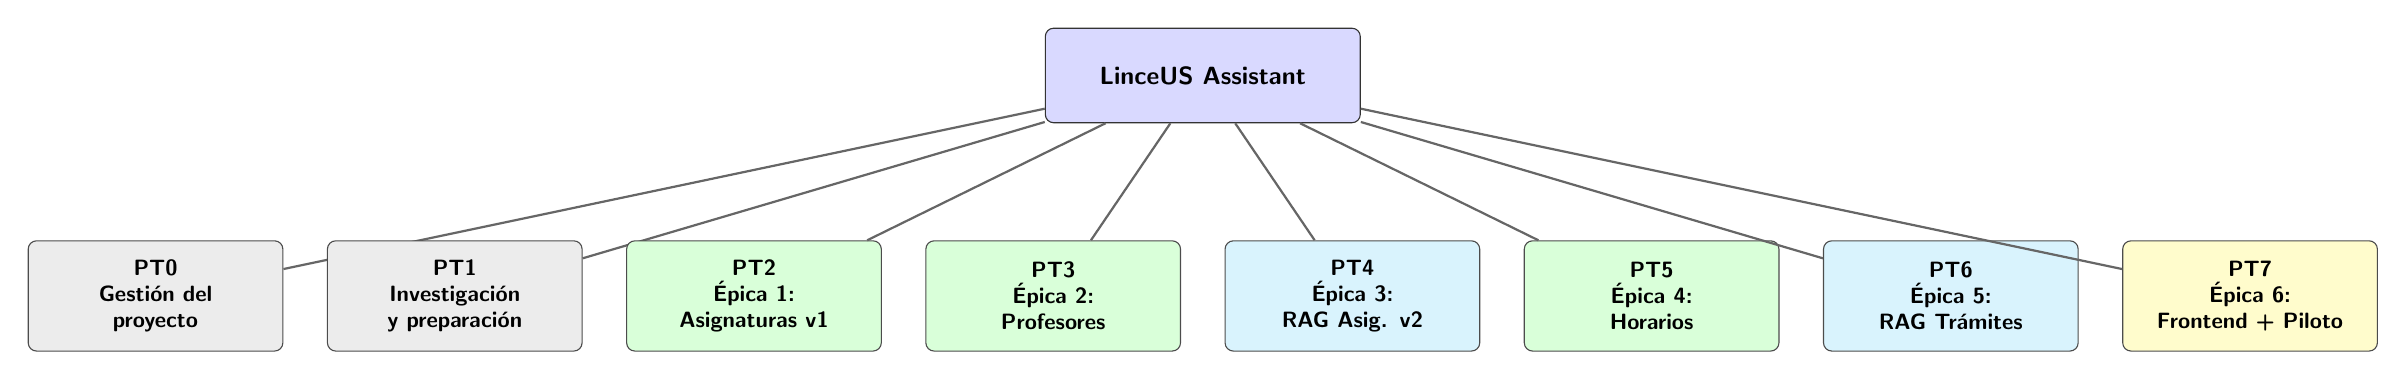
\begin{tikzpicture}[
    level 1/.style={sibling distance=38mm, level distance=28mm},
    every node/.style={font=\small\sffamily},
    root/.style={rectangle, draw=black!80, fill=blue!15, minimum width=40mm, minimum height=12mm, align=center, font=\small\sffamily\bfseries, rounded corners=3pt},
    pkg/.style={rectangle, draw=black!70, fill=#1, minimum width=32mm, minimum height=14mm, align=center, font=\footnotesize\sffamily\bfseries, rounded corners=3pt, text width=30mm},
    pkg/.default={orange!15},
    tasks/.style={font=\scriptsize\sffamily, text=black!60, align=center},
    edge from parent/.style={draw=black!60, thick}
]

\node[root] {LinceUS Assistant}
    child { node[pkg=gray!15] {PT0\\Gestión del\\proyecto} }
    child { node[pkg=gray!15] {PT1\\Investigación\\y preparación} }
    child { node[pkg=green!15] {PT2\\Épica 1:\\Asignaturas v1} }
    child { node[pkg=green!15] {PT3\\Épica 2:\\Profesores} }
    child { node[pkg=cyan!15] {PT4\\Épica 3:\\RAG Asig. v2} }
    child { node[pkg=green!15] {PT5\\Épica 4:\\Horarios} }
    child { node[pkg=cyan!15] {PT6\\Épica 5:\\RAG Trámites} }
    child { node[pkg=yellow!20] {PT7\\Épica 6:\\Frontend + Piloto} }
;

\end{tikzpicture}
}%
\caption{Estructura de Descomposición del Trabajo (EDT) — nivel de paquetes de trabajo.}
\label{fig:edt}
\end{figure}

% =====================================================
% SECCIÓN 2: DICCIONARIO EDT
% =====================================================

\section{Diccionario EDT}\label{sec:diccionario-edt}

El diccionario EDT define cada paquete de trabajo y sus tareas constituyentes, especificando su descripción, entregables y estimación de esfuerzo. Las estimaciones siguen la escala: \textbf{S} (Small, $\leq$1 semana), \textbf{M} (Medium, 1--2 semanas) y \textbf{L} (Large, 2--3 semanas).

% --- PT0 ---
\subsection{PT0 — Gestión del proyecto}\label{subsec:pt0}

Paquete transversal que abarca la planificación, seguimiento y documentación formal del proyecto a lo largo de todo su ciclo de vida.

\begin{table}[hbtp]
\centering
\small
\begin{tabular}{|l|l|p{7.5cm}|c|}
\hline
\textbf{ID} & \textbf{Tarea} & \textbf{Descripción y entregables} & \textbf{Est.} \\ \hline
0.1 & Planificación y seguimiento & Definición del alcance, elaboración de la EDT, planificación de sprints, seguimiento del progreso y gestión de riesgos. \textit{Entregable: anteproyecto, actas de seguimiento.} & L \\ \hline
0.2 & Redacción de la memoria & Redacción continua de la memoria del TFG: introducción, marco teórico, metodología, diseño, implementación, pruebas y conclusiones. \textit{Entregable: memoria del TFG.} & L \\ \hline
0.3 & Preparación de la defensa & Elaboración de las diapositivas de presentación, ensayo de la defensa y preparación de la demostración en vivo. \textit{Entregable: presentación, demo.} & M \\ \hline
\end{tabular}
\caption{Diccionario EDT — PT0: Gestión del proyecto.}
\label{tab:dict-pt0}
\end{table}

% --- PT1 ---
\subsection{PT1 — Investigación y preparación}\label{subsec:pt1}

Paquete que recoge el trabajo previo de investigación tecnológica, toma de decisiones y configuración del entorno de desarrollo.

\begin{table}[hbtp]
\centering
\small
\begin{tabular}{|l|l|p{7.5cm}|c|}
\hline
\textbf{ID} & \textbf{Tarea} & \textbf{Descripción y entregables} & \textbf{Est.} \\ \hline
1.1 & Estudio de tecnologías & Análisis comparativo de frameworks conversacionales (Rasa, Botpress, DeepPavlov), bases de datos (Supabase, PostgreSQL, motores vectoriales) y APIs de LLM (Gemini, OpenAI, DeepSeek). \textit{Entregable: tablas comparativas, decisión documentada.} & L \\ \hline
1.2 & Setup del entorno & Instalación y configuración de Python, Rasa, Supabase, Gemini API, Git/GitHub. Creación del repositorio y estructura inicial del proyecto. \textit{Entregable: entorno funcional, repositorio.} & M \\ \hline
1.3 & Diseño de la arquitectura & Definición de la arquitectura por capas, diseño de la base de datos, definición de interfaces entre componentes y protocolos de comunicación. \textit{Entregable: diagramas de arquitectura, esquema ER.} & M \\ \hline
\end{tabular}
\caption{Diccionario EDT — PT1: Investigación y preparación.}
\label{tab:dict-pt1}
\end{table}

% --- PT2 ---
\subsection{PT2 — Épica 1: Asignaturas v1 (BD estructurada)}\label{subsec:pt2}

Primera épica de desarrollo. Implementa la consulta de información básica de asignaturas (código, nombre, curso, créditos, tipología, duración) mediante consultas SQL sobre la base de datos estructurada, sin RAG.

\begin{table}[hbtp]
\centering
\small
\begin{tabular}{|l|l|p{7.5cm}|c|}
\hline
\textbf{ID} & \textbf{Tarea} & \textbf{Descripción y entregables} & \textbf{Est.} \\ \hline
2.1 & Esquema de datos en Supabase & Definir tablas de asignaturas (código, nombre, curso, créditos, tipología, duración) con restricciones de integridad y relaciones. \textit{Entregable: script SQL de creación.} & S \\ \hline
2.2 & Script de carga CSV + plantilla & Script Python/SQL con upsert, validaciones de obligatorios, tipos, duplicados y tildes. Plantilla vacía para nuevas titulaciones. \textit{Entregable: script de carga, plantilla CSV.} & M \\ \hline
2.3 & Ingesta del curso objetivo & Cargar $\sim$9 asignaturas del curso elegido (ETSII) y verificar integridad y relaciones. \textit{Entregable: datos cargados y validados.} & M \\ \hline
2.4 & Intents y entidades de consulta & Definir intents y entidades para ``calificación/evaluación/metodología/bibliografía de X'' con variaciones coloquiales y sinónimos. \textit{Entregable: ficheros NLU en YAML.} & M \\ \hline
2.5 & Acción Rasa (SQL) & Acción personalizada con consulta parametrizada a Supabase, normalización de nombres (fuzzy matching) y formateo de respuesta con fallback. \textit{Entregable: módulo actions.} & L \\ \hline
2.6 & Testing de la épica & Golden set $\geq$30 casos, unit tests y end-to-end. Objetivo: $\geq$90\% de acierto. \textit{Entregable: suite de tests, informe de resultados.} & M \\ \hline
2.7 & Documentación breve & Diagrama ER de datos y guía reproducible de carga (pasos y validaciones). \textit{Entregable: documentación técnica.} & S \\ \hline
2.8 & Preparación de RAG (inventario) & Lista de fuentes para proyectos docentes y criterios de inclusión/versión. \textit{Entregable: inventario de fuentes.} & L \\ \hline
\end{tabular}
\caption{Diccionario EDT — PT2: Épica 1 — Asignaturas v1.}
\label{tab:dict-pt2}
\end{table}

% --- PT3 ---
\subsection{PT3 — Épica 2: Profesores}\label{subsec:pt3}

Segunda épica. Permite consultar datos de contacto, despacho y horarios de tutorías del profesorado, con búsqueda por nombre o por asignatura.

\begin{table}[hbtp]
\centering
\small
\begin{tabular}{|l|l|p{7.5cm}|c|}
\hline
\textbf{ID} & \textbf{Tarea} & \textbf{Descripción y entregables} & \textbf{Est.} \\ \hline
3.1 & Esquema profesores/tutorías & Tablas \texttt{profesores} (nombre, departamento, correo, despacho) y \texttt{tutorias} (día, hora, modalidad) con FK hacia asignaturas. \textit{Entregable: script SQL.} & S \\ \hline
3.2 & Carga y normalización & Cargar CSV de profesores y tutorías; normalizar alias, tildes y abreviaturas; control de duplicados. \textit{Entregable: datos cargados.} & M \\ \hline
3.3 & Intents y entidades & Definir intents para ``Correo de\ldots'', ``Despacho de\ldots'', ``Tutorías de\ldots'' y ``¿Quién da [Asignatura]?''. \textit{Entregable: ficheros NLU.} & L \\ \hline
3.4 & Acciones SQL & Consultas por nombre y por asignatura; manejo de ambigüedades (varios profesores con nombre similar). \textit{Entregable: módulo actions.} & L \\ \hline
3.5 & Testing de la épica & Golden set $\geq$20 casos; $\geq$95\% de acierto; casos de alias y errores ortográficos menores. \textit{Entregable: suite de tests.} & M \\ \hline
\end{tabular}
\caption{Diccionario EDT — PT3: Épica 2 — Profesores.}
\label{tab:dict-pt3}
\end{table}

% --- PT4 ---
\subsection{PT4 — Épica 3: RAG Asignaturas v2}\label{subsec:pt4}

Tercera épica. Extiende la consulta de asignaturas con información extraída de los proyectos docentes (PDF) mediante técnicas de RAG: extracción, chunking, embeddings y búsqueda semántica.

\begin{table}[hbtp]
\centering
\small
\begin{tabular}{|l|l|p{7.5cm}|c|}
\hline
\textbf{ID} & \textbf{Tarea} & \textbf{Descripción y entregables} & \textbf{Est.} \\ \hline
4.1 & Inventario de fuentes & Mapa de proyectos docentes (URLs/PDF) y decisión de extracción (scraping vs curación manual). \textit{Entregable: inventario documentado.} & M \\ \hline
4.2 & Extracción y chunking & Parseo de PDF con pdfplumber, chunking semántico (800 caracteres, 100 de solapamiento) y metadatos (asignatura, año, sección, fecha de vigencia). \textit{Entregable: pipeline de extracción.} & M \\ \hline
4.3 & Embeddings en Supabase & Generación de embeddings con Gemini (\texttt{gemini-embedding-001}, 2000 dimensiones) y almacenamiento en pgvector con índices HNSW. \textit{Entregable: pipeline de vectorización.} & M \\ \hline
4.4 & Acción RAG con citas & Retrieval semántico + fallback por keywords; respuesta con cita (documento y sección) y umbral de confianza con fallback a enlaces útiles. \textit{Entregable: acción RAG integrada.} & L \\ \hline
4.5 & Testing de la épica & Anti-alucinación con golden set $\geq$40 casos, $\geq$90\% de precisión factual, pruebas de no-regresión al actualizar documentos. \textit{Entregable: suite de tests.} & M \\ \hline
\end{tabular}
\caption{Diccionario EDT — PT4: Épica 3 — RAG Asignaturas v2.}
\label{tab:dict-pt4}
\end{table}

% --- PT5 ---
\subsection{PT5 — Épica 4: Horarios}\label{subsec:pt5}

Cuarta épica. Permite consultar horarios de clases mediante una base de datos relacional con grupos, tramos horarios y aulas.

\begin{table}[hbtp]
\centering
\small
\begin{tabular}{|l|l|p{7.5cm}|c|}
\hline
\textbf{ID} & \textbf{Tarea} & \textbf{Descripción y entregables} & \textbf{Est.} \\ \hline
5.1 & Esquema horarios & Tablas \texttt{grupos\_clase}, \texttt{horarios} y \texttt{aulas} con claves foráneas y validación de solapes horarios. \textit{Entregable: script SQL.} & M \\ \hline
5.2 & Carga del curso & Cargar 1 curso ($\approx$4 grupos $\times$ 9 asignaturas) con validaciones de consistencia temporal. \textit{Entregable: datos cargados.} & S \\ \hline
5.3 & Intents y acciones & Consultas por asignatura, grupo y curso; formateo en tabla legible. \textit{Entregable: intents NLU y acciones Python.} & L \\ \hline
5.4 & Export CSV (opcional) & Exportar CSV del horario personal del alumno, si entra en alcance. \textit{Entregable: funcionalidad de exportación.} & L \\ \hline
5.5 & Testing de la épica & Golden set $\geq$30 casos; pruebas de rendimiento y de formato de salida. \textit{Entregable: suite de tests.} & M \\ \hline
\end{tabular}
\caption{Diccionario EDT — PT5: Épica 4 — Horarios.}
\label{tab:dict-pt5}
\end{table}

% --- PT6 ---
\subsection{PT6 — Épica 5: RAG Trámites}\label{subsec:pt6}

Quinta épica. Permite consultar información sobre trámites administrativos (matrícula, becas, certificados, convalidaciones) mediante RAG sobre páginas oficiales y documentos institucionales.

\begin{table}[hbtp]
\centering
\small
\begin{tabular}{|l|l|p{7.5cm}|c|}
\hline
\textbf{ID} & \textbf{Tarea} & \textbf{Descripción y entregables} & \textbf{Est.} \\ \hline
6.1 & Mapa de páginas & Identificar páginas oficiales y documentos relevantes; registrar fecha de vigencia de cada fuente. \textit{Entregable: mapa de fuentes.} & M \\ \hline
6.2 & Extracción/curación + chunking & Extraer contenido de webs y PDFs, normalizar, chunking con metacampos (tema, fecha, URL de origen). \textit{Entregable: pipeline de extracción.} & L \\ \hline
6.3 & Embeddings + acción RAG & Cargar embeddings; acción que siempre muestre fuente y fecha, y gestione discrepancias entre fuentes. \textit{Entregable: acción RAG de trámites.} & L \\ \hline
6.4 & Testing de la épica & Golden set $\geq$40 casos, pruebas de no-regresión y verificación de enlaces; $\geq$90\% de precisión factual. \textit{Entregable: suite de tests.} & M \\ \hline
\end{tabular}
\caption{Diccionario EDT — PT6: Épica 5 — RAG Trámites.}
\label{tab:dict-pt6}
\end{table}

% --- PT7 ---
\subsection{PT7 — Épica 6: Frontend + Piloto + Entrega}\label{subsec:pt7}

Sexta épica. Abarca el desarrollo de la interfaz web, la ejecución de un piloto con usuarios reales y la finalización de la documentación para la entrega.

\begin{table}[hbtp]
\centering
\small
\begin{tabular}{|l|l|p{7.5cm}|c|}
\hline
\textbf{ID} & \textbf{Tarea} & \textbf{Descripción y entregables} & \textbf{Est.} \\ \hline
7.1 & UI del widget web & Chat web conectado a Rasa mediante API REST; renderizado de respuestas enriquecidas (Markdown, tablas); accesibilidad básica (WCAG). \textit{Entregable: widget JS embebible.} & S \\ \hline
7.2 & Piloto y ajustes & Piloto con 5--10 estudiantes, recogida de feedback y ajustes de UX y flujos conversacionales; corrección de regresiones. \textit{Entregable: informe del piloto.} & M \\ \hline
7.3 & Memoria y defensa & Redacción final de la memoria (metodología, arquitectura, evaluación), elaboración de diapositivas y ensayo de defensa con métricas. \textit{Entregable: memoria final, presentación.} & L \\ \hline
\end{tabular}
\caption{Diccionario EDT — PT7: Épica 6 — Frontend + Piloto + Entrega.}
\label{tab:dict-pt7}
\end{table}

% =====================================================
% SECCIÓN 3: RESUMEN DE LA EDT
% =====================================================

\section{Resumen cuantitativo de la EDT}\label{sec:resumen-edt}

La Tabla~\ref{tab:resumen-edt} resume los paquetes de trabajo, el número de tareas y la distribución de esfuerzo estimada.

\begin{table}[hbtp]
\centering
\begin{tabular}{|l|l|c|c|c|c|}
\hline
\textbf{ID} & \textbf{Paquete de trabajo} & \textbf{Tareas} & \textbf{S} & \textbf{M} & \textbf{L} \\ \hline
PT0 & Gestión del proyecto & 3 & 0 & 1 & 2 \\ \hline
PT1 & Investigación y preparación & 3 & 0 & 2 & 1 \\ \hline
PT2 & Épica 1: Asignaturas v1 & 8 & 2 & 4 & 2 \\ \hline
PT3 & Épica 2: Profesores & 5 & 1 & 2 & 2 \\ \hline
PT4 & Épica 3: RAG Asignaturas v2 & 5 & 0 & 3 & 2 \\ \hline
PT5 & Épica 4: Horarios & 5 & 1 & 2 & 2 \\ \hline
PT6 & Épica 5: RAG Trámites & 4 & 0 & 2 & 2 \\ \hline
PT7 & Épica 6: Frontend + Piloto & 3 & 1 & 1 & 1 \\ \hline
\hline
\multicolumn{2}{|l|}{\textbf{Total}} & \textbf{36} & \textbf{5} & \textbf{17} & \textbf{14} \\ \hline
\end{tabular}
\caption{Resumen cuantitativo de la EDT por paquete de trabajo.}
\label{tab:resumen-edt}
\end{table}

% =====================================================
% SECCIÓN 4: BACKLOG
% =====================================================

\section{Backlog del producto}\label{sec:backlog}

El backlog del producto se deriva directamente de la EDT y organiza las épicas de desarrollo por prioridad. Cada épica se implementa de forma secuencial, de modo que las funcionalidades se entregan de forma incremental siguiendo el marco SCRUM adaptado descrito en el Capítulo~\ref{cap:metodologia}.

La priorización responde a dos criterios:

\begin{enumerate}
    \item \textbf{Valor para el usuario}: Las épicas que cubren las consultas más frecuentes de los estudiantes (asignaturas, profesorado) se implementan primero.
    \item \textbf{Dependencia técnica}: Las épicas que requieren infraestructura previa (como RAG, que depende de la base de datos vectorial) se planifican después de que dicha infraestructura esté operativa.
\end{enumerate}

La Tabla~\ref{tab:backlog-prioridad} muestra el orden de prioridad de las épicas.

\begin{table}[hbtp]
\centering
\begin{tabular}{|c|l|l|c|}
\hline
\textbf{Prioridad} & \textbf{Épica} & \textbf{Dependencia} & \textbf{Sprints est.} \\ \hline
1 & Asignaturas v1 (BD estructurada) & --- & S1--S8 \\ \hline
2 & Profesores (contacto, tutorías) & Épica 1 (esquema BD) & S9--S12 \\ \hline
3 & RAG Asignaturas v2 (proyectos docentes) & Épica 1 (inventario fuentes) & S12--S14 \\ \hline
4 & Horarios (BD relacional) & Épica 2 (profesores) & S15--S16 \\ \hline
5 & RAG Trámites & Épica 3 (pipeline RAG) & S17--S19 \\ \hline
6 & Frontend + Piloto + Entrega & Todas las anteriores & S19--S21 \\ \hline
\end{tabular}
\caption{Priorización del backlog por épicas.}
\label{tab:backlog-prioridad}
\end{table}

% =====================================================
% SECCIÓN 5: PLANIFICACIÓN DE SPRINTS
% =====================================================

\section{Planificación de sprints}\label{sec:sprints}

El proyecto se organiza en sprints de \textbf{3--4 semanas de duración}, siguiendo una adaptación de SCRUM para un proyecto individual (véase Capítulo~\ref{cap:metodologia}). Cada sprint tiene un objetivo definido y produce un incremento funcional del sistema.

% TODO: Completar con los sprints reales ejecutados y sus resultados

% =====================================================
% SECCIÓN 6: CRONOGRAMA
% =====================================================

\section{Cronograma}\label{sec:cronograma}

% TODO: Añadir diagrama de Gantt o cronograma temporal con los hitos principales del proyecto


% =====================================================
% PARTE III: DISEÑO E IMPLEMENTACIÓN
% =====================================================
\part{Diseño e Implementación}

     % !TEX root = ../proyect.tex

\chapter{Análisis de requisitos}\label{cap:requisitos}

Este capítulo recoge el análisis de requisitos del sistema Linceus Assistant en su versión correspondiente al cierre del prototipo (fase 1). El análisis ha sido un proceso iterativo: la propuesta inicial planteaba un alcance amplio que incluía notificaciones a estudiantes, soporte multilingüe e integraciones en tiempo real con plataformas institucionales, pero la limitación de tiempo propia de un trabajo individual ha obligado a priorizar el núcleo conversacional y el dominio académico, y a aplazar el resto a iteraciones posteriores. La sección~\ref{sec:req-evolucion} cierra el capítulo precisamente con un repaso de cómo ha evolucionado el alcance respecto del documento original, dado que la guía de referencia~\cite{segura2024guiatfg} recomienda dejar trazabilidad de las desviaciones de planificación.

Los requisitos se organizan en cuatro tipos siguiendo la práctica habitual en ingeniería del software: requisitos funcionales (qué hace el sistema), requisitos de información (qué datos maneja), requisitos no funcionales (con qué calidad lo hace) y prototipos de interfaz (cómo se muestra al usuario). Cada requisito funcional se acompaña, cuando procede, de los identificadores de los casos de prueba que lo verifican, lo que permite cruzarlo con el Capítulo~\ref{cap:pruebas}.

\section{Identificación de actores}\label{sec:req-actores}

El sistema atiende a tres tipos de usuarios bien diferenciados, que justifican la estructura de los manuales recogida en el Capítulo~\ref{cap:manuales}.

El \textbf{estudiante} es el usuario principal del prototipo. Comprende tanto al alumnado matriculado en la ETSII como al alumnado de nuevo ingreso o internacional que utiliza el sistema antes de iniciar el curso. Interactúa con el bot a través del \textit{widget} integrado en la página principal, sin necesidad de autenticación, y formula consultas en español natural sobre asignaturas, horarios y profesorado.

El \textbf{administrador del sistema} es el perfil técnico encargado de mantener actualizada la base de conocimiento. Su interacción se realiza exclusivamente a través del panel de administración (puerto 5050), e incluye la sincronización de centros, titulaciones y asignaturas desde Sevius, la vectorización de planes docentes en el módulo RAG y la auditoría de las conversaciones registradas durante el piloto. La existencia del panel obedece principalmente a un requisito de \textbf{mantenibilidad y escalabilidad}: el sistema debe poder ser asumido por otra persona tras el cierre del TFG sin necesidad de manipular directamente la base de datos.

El \textbf{desarrollador} es el perfil destinado a continuar el proyecto en futuras iteraciones. Consume el repositorio, las convenciones documentadas y los registros de decisiones técnicas para incorporar nuevas intenciones, ampliar el dominio o modificar las acciones existentes. Sus requisitos se materializan en buenas prácticas y trazabilidad, no en funcionalidades específicas del producto.

\section{Requisitos funcionales}\label{sec:req-funcionales}

Los requisitos funcionales se agrupan por dominio. La columna \textit{Pruebas} de cada tabla indica los identificadores de los casos de aceptación que verifican el requisito en el Capítulo~\ref{cap:pruebas}.

\subsection{Dominio de asignaturas}\label{subsec:rf-asignaturas}

\begin{table}[hbtp]
\centering
\small
\caption{Requisitos funcionales del dominio de asignaturas.}\label{tab:rf-asignaturas}
\begin{tabular}{|p{1.1cm}|p{8.2cm}|p{1.0cm}|p{2.0cm}|}
\hline
\textbf{ID} & \textbf{Descripción} & \textbf{Prio.} & \textbf{Pruebas} \\ \hline
RF-A1 & El sistema debe responder con la ficha completa de una asignatura cuando el usuario la nombra de forma explícita o mediante alias o acrónimo (ADDA, FP, IISSI2). & Alta & E-P01..E-P12 \\ \hline
RF-A2 & El sistema debe devolver listados de asignaturas filtrados por curso, cuatrimestre, tipo (formación básica, obligatoria, optativa) o créditos. & Alta & L-P01..L-P10 \\ \hline
RF-A3 & El sistema debe responder al conteo de asignaturas que cumplan un criterio dado. & Media & C-P01..C-T02 \\ \hline
RF-A4 & El sistema debe recuperar información del plan docente (criterios de evaluación, profesorado, bloques, idioma, tribunales) mediante el módulo RAG. & Alta & §\ref{subsec:rag-profundidad} \\ \hline
RF-A5 & El sistema debe heredar el contexto cuando una consulta elíptica (``y cuántos créditos tiene?'') se refiere a la última asignatura mencionada. & Media & E-S01..E-S03 \\ \hline
RF-A6 & El sistema debe resolver consultas multi-asignatura en un único turno (``cómo se evalúan DP1 y PSG2''). & Media & E-M01 \\ \hline
RF-A7 & El sistema debe distinguir entre la pregunta ``qué es X'' (ficha) y ``cuándo es X'' (horario), aun cuando ambas comparten léxico. & Alta & E-P09, HA-P01 \\ \hline
\end{tabular}
\end{table}

\subsection{Dominio de horarios}\label{subsec:rf-horarios}

\begin{table}[hbtp]
\centering
\small
\caption{Requisitos funcionales del dominio de horarios.}\label{tab:rf-horarios}
\begin{tabular}{|p{1.1cm}|p{8.2cm}|p{1.0cm}|p{2.0cm}|}
\hline
\textbf{ID} & \textbf{Descripción} & \textbf{Prio.} & \textbf{Pruebas} \\ \hline
RF-H1 & El sistema debe devolver el horario semanal de un curso y grupo dados. & Alta & H-P01..H-P11 \\ \hline
RF-H2 & El sistema debe devolver el horario filtrado por día de la semana. & Alta & H-P01, H-P10 \\ \hline
RF-H3 & El sistema debe filtrar el horario por cuatrimestre cuando el usuario lo especifica. & Media & H-PC01..H-PC03 \\ \hline
RF-H4 & El sistema debe responder al horario de una asignatura concreta sin requerir curso ni grupo. & Alta & HA-P01..HA-P12 \\ \hline
RF-H5 & El sistema debe distinguir aulas de teoría de aulas de laboratorio cuando el usuario lo solicita expresamente. & Media & HA-P11 \\ \hline
RF-H6 & El sistema debe solicitar curso y grupo cuando la consulta los requiere y faltan en el mensaje. & Alta & H-P10, H-P12 \\ \hline
RF-H7 & El sistema debe rechazar de manera explícita consultas con curso o grupo inexistentes (curso 8, grupo 15). & Media & H-N01, H-N02 \\ \hline
\end{tabular}
\end{table}

\subsection{Dominio de profesorado}\label{subsec:rf-profesorado}

\begin{table}[hbtp]
\centering
\small
\caption{Requisitos funcionales del dominio de profesorado.}\label{tab:rf-profesorado}
\begin{tabular}{|p{1.1cm}|p{8.2cm}|p{1.0cm}|p{2.0cm}|}
\hline
\textbf{ID} & \textbf{Descripción} & \textbf{Prio.} & \textbf{Pruebas} \\ \hline
RF-P1 & El sistema debe devolver los datos de contacto de un profesor (email, despacho, teléfono, web personal) por nombre o apellido. & Alta & P-P01..P-P10 \\ \hline
RF-P2 & El sistema debe listar el profesorado que imparte una asignatura. & Alta & P-PA01..P-PA08 \\ \hline
RF-P3 & El sistema debe identificar al coordinador y a los suplentes de una asignatura mediante recuperación semántica sobre el plan docente. & Alta & P-PA05..P-PA08 \\ \hline
RF-P4 & El sistema debe responder a consultas sobre tutorías redirigiendo al correo del profesor (decisión de diseño documentada en D-061). & Media & P-T01..P-T05 \\ \hline
RF-P5 & El sistema debe permitir filtrar el profesorado de un departamento concreto. & Media & P-P10 \\ \hline
RF-P6 & El sistema debe tolerar errores tipográficos moderados en nombres de profesores (``parejjo'', ``galinndo''). & Media & P-W01..P-W07 \\ \hline
RF-P7 & El sistema debe declarar explícitamente la ausencia de información cuando un profesor no figura en la base de datos, sin inventar contenido. & Alta & P-N01..P-N04 \\ \hline
\end{tabular}
\end{table}

\subsection{Comportamientos transversales}\label{subsec:rf-transversal}

\begin{table}[hbtp]
\centering
\small
\caption{Requisitos funcionales transversales.}\label{tab:rf-transversal}
\begin{tabular}{|p{1.1cm}|p{8.2cm}|p{1.0cm}|p{2.0cm}|}
\hline
\textbf{ID} & \textbf{Descripción} & \textbf{Prio.} & \textbf{Pruebas} \\ \hline
RF-T1 & El sistema debe permitir cambiar dinámicamente la titulación activa durante una conversación, ya sea desde el selector o mediante lenguaje natural. & Alta & CC-P01..CC-P11 \\ \hline
RF-T2 & El sistema debe rechazar titulaciones fuera del alcance ETSII con un mensaje explícito (\textit{cambia a Biología}). & Alta & CC-N01 \\ \hline
RF-T3 & El sistema debe identificar consultas fuera de ámbito (clima, peticiones generales) y responder de forma cortés sin entrar al pipeline de consulta académica. & Alta & F-01..F-04 \\ \hline
RF-T4 & El sistema debe bloquear intentos de \textit{prompt injection} y \textit{jailbreak} (``ignora las instrucciones anteriores''). & Alta & R-01..R-04 \\ \hline
RF-T5 & El sistema debe ofrecer un mensaje de bienvenida y soportar la pregunta meta-conversacional ``¿qué eres?'' redirigiendo a la naturaleza del bot. & Media & R-04 \\ \hline
RF-T6 & El sistema debe permitir al usuario reportar respuestas incorrectas mediante un mecanismo de \textit{feedback} integrado en el \textit{widget}. & Media & --- \\ \hline
\end{tabular}
\end{table}

\subsection{Funcionalidades del panel de administración}\label{subsec:rf-admin}

El panel de administración no se ofrece al estudiante final, sino al perfil de administrador descrito en la Sección~\ref{sec:req-actores}. Su existencia responde a un requisito de mantenibilidad: garantizar que la persona que asuma la continuidad del sistema pueda gestionar los datos sin necesidad de manipular directamente la base de datos. Los requisitos se recogen en la Tabla~\ref{tab:rf-admin}.

\begin{table}[hbtp]
\centering
\small
\caption{Requisitos funcionales del panel de administración.}\label{tab:rf-admin}
\begin{tabular}{|p{1.1cm}|p{8.2cm}|p{1.0cm}|}
\hline
\textbf{ID} & \textbf{Descripción} & \textbf{Prio.} \\ \hline
RF-AD1 & El panel debe permitir la navegación jerárquica Centro $\rightarrow$ Titulación $\rightarrow$ Asignatura sobre los datos cargados (D-037). & Alta \\ \hline
RF-AD2 & El panel debe ofrecer la sincronización de centros, titulaciones y asignaturas desde Sevius como fuente de verdad institucional, mediante un flujo \textit{preview-first} (D-038, D-039). & Alta \\ \hline
RF-AD3 & El panel debe permitir vectorizar el plan docente de una asignatura, integrándolo en el corpus de \textit{embeddings} consumido por el módulo RAG (D-040, D-041). & Alta \\ \hline
RF-AD4 & El panel debe importar y enriquecer profesorado a partir del directorio PDI de \texttt{us.es} usando el filtro de centro (D-043, D-044). & Media \\ \hline
RF-AD5 & El panel debe ofrecer una vista jerárquica Centro $\rightarrow$ Departamento $\rightarrow$ Profesor, con un \textit{bucket} para profesores sin departamento asignado (D-051). & Media \\ \hline
RF-AD6 & El panel debe exponer las conversaciones registradas en \texttt{conversation\_log} para revisión manual del evaluador, con la posibilidad de marcarlas como revisadas. & Alta \\ \hline
RF-AD7 & El panel debe agregar el \textit{feedback} explícito por turno aportado por los usuarios y permitir su consulta agregada. & Media \\ \hline
\end{tabular}
\end{table}

\section{Requisitos de información}\label{sec:req-informacion}

El modelo de información del sistema se estructura en torno a tres bloques. El primero recoge los datos de \textbf{dominio académico} consumidos por el bot, que son la fuente de verdad para responder a las consultas del usuario. El segundo recoge los datos del \textbf{módulo RAG}, esto es, los fragmentos vectorizados de los planes docentes con sus respectivos \textit{embeddings}. El tercero recoge los datos de \textbf{operación}, es decir, las conversaciones registradas durante el piloto y el \textit{feedback} explícito asociado.

\subsection{Entidades de dominio}\label{subsec:ri-dominio}

Las entidades del dominio académico son las recogidas en la Tabla~\ref{tab:ri-dominio}. La descripción técnica completa de cada tabla, con sus tipos, claves y restricciones, figura en el Capítulo~\ref{cap:estructura-bd}.

\begin{table}[hbtp]
\centering
\small
\caption{Entidades de información del dominio académico.}\label{tab:ri-dominio}
\begin{tabular}{|p{2.8cm}|p{9.0cm}|}
\hline
\textbf{Entidad} & \textbf{Descripción} \\ \hline
Centro & Unidad organizativa que agrupa titulaciones (ETSII). \\ \hline
Titulación & Plan de estudios (GII-IS, GII-IC, GII-TI). \\ \hline
Asignatura & Materia con su código, créditos, curso, cuatrimestre y tipo. \\ \hline
Departamento & Unidad académica responsable del profesorado. \\ \hline
Profesor & Docente con datos de contacto, despacho y departamento. \\ \hline
Profesor-Asignatura & Relación que vincula un profesor con la docencia de una asignatura, con el grupo y el rol (titular, coordinador, suplente). \\ \hline
Grupo de clase & Asignatura impartida en un grupo concreto a un curso. \\ \hline
Aula & Espacio físico identificado por código (A0.10, B1.31, F1.30) y tipo (teoría/laboratorio). \\ \hline
Horario & Sesión docente que vincula grupo, aula, día, franja horaria y cuatrimestre. \\ \hline
Plan docente & Documento PDF oficial asociado a una asignatura, fuente del corpus RAG. \\ \hline
\end{tabular}
\end{table}

\subsection{Entidades del módulo RAG}\label{subsec:ri-rag}

El módulo RAG opera sobre fragmentos textuales (\textit{chunks}) extraídos de los planes docentes. Cada \textit{chunk} se almacena junto con su \textit{embedding} vectorial calculado con el modelo de \textit{embeddings} de Gemini, y con un conjunto de metadatos que permiten filtrar y reordenar resultados durante la recuperación: titulación, asignatura, sección del plan docente (profesorado, evaluación, bloques, etc.), grupo y curso. La sección como metadato fue una decisión de diseño documentada (D-031, D-058.b): se usa como señal para reordenar resultados pero no como filtro estricto, dado que la sección de origen no siempre es informativa para responder a la pregunta.

\subsection{Entidades de operación}\label{subsec:ri-operacion}

La operación del sistema en producción registra dos entidades. La tabla \texttt{conversation\_log} almacena turno a turno cada interacción con el bot: identificador anónimo de sesión, mensaje del usuario, \textit{intent} clasificado, \textit{slots} activos, respuesta del bot, indicador de revisión manual y marca temporal. La tabla \texttt{feedback} recoge la valoración explícita del usuario sobre un turno concreto cuando este utiliza los botones de aprobación o rechazo del \textit{widget}. Ninguna de las dos almacena datos personales identificables, dado que la sesión es anónima por diseño.

\section{Requisitos no funcionales}\label{sec:req-no-funcionales}

Los requisitos no funcionales se enuncian en términos medibles y se cruzan con la evidencia recogida en el Capítulo~\ref{cap:pruebas}. Los umbrales son los que el equipo del TFG considera aceptables para un prototipo de fase 1 desplegable a la población de la ETSII; se han ajustado durante el desarrollo a la luz de las cifras observadas durante el piloto.

\begin{table}[hbtp]
\centering
\small
\caption{Requisitos no funcionales y evidencia.}\label{tab:rnf}
\begin{tabular}{|p{1.4cm}|p{4.5cm}|p{4.0cm}|p{2.5cm}|}
\hline
\textbf{ID} & \textbf{Descripción} & \textbf{Umbral} & \textbf{Evidencia} \\ \hline
RNF-1 & Latencia mediana de respuesta extremo a extremo. & p50 $\leq$ 4~s & §\ref{subsec:no-funcional-latencia} (3,4~s) \\ \hline
RNF-2 & Latencia en cola larga. & p95 $\leq$ 12~s & §\ref{subsec:no-funcional-latencia} (10,5~s) \\ \hline
RNF-3 & Coste medio por turno (servicio Gemini). & $\leq$ 0,05 cts & §\ref{subsec:no-funcional-coste} (0,012~cts) \\ \hline
RNF-4 & Tasa de éxito en suite de aceptación E2E. & $\geq$ 90~\% & §\ref{sec:pruebas-e2e} (94,3~\%) \\ \hline
RNF-5 & Tasa de éxito sobre tráfico real post-despliegue. & $\geq$ 85~\% & §\ref{sec:pruebas-trafico} (98,3~\%) \\ \hline
RNF-6 & Disponibilidad del servicio. & $\geq$ 99~\% mensual & Pendiente fase 2 \\ \hline
RNF-7 & Idioma soportado. & Español peninsular & Validado en piloto \\ \hline
RNF-8 & Compatibilidad de navegadores. & Chrome, Firefox, Edge y Safari modernos. & Verificado manualmente \\ \hline
RNF-9 & Diseño \textit{responsive} en dispositivos móviles. & Funcional en pantallas $\geq$ 320~px. & Verificado manualmente \\ \hline
RNF-10 & Anonimato del usuario y ausencia de PII. & Sesiones identificadas mediante UUID anónimo. & Por diseño \\ \hline
RNF-11 & Reproducibilidad del despliegue. & \textit{Stack} levantable mediante \texttt{docker compose up}. & §\ref{sec:manual-despliegue} \\ \hline
RNF-12 & Trazabilidad de decisiones técnicas. & Registro en \texttt{docs/sprints/}. & Sprints S2--S7 \\ \hline
\end{tabular}
\end{table}

Conviene comentar dos requisitos en particular. El cumplimiento de la \textbf{normativa de protección de datos} (RNF-10) se materializa por construcción más que por restricciones de despliegue: el sistema no requiere autenticación, no almacena datos personales identificables, y los datos académicos consultados (planes docentes, horarios, directorio de profesorado) son de carácter público y proceden de fuentes oficiales (Sevius, \texttt{us.es}). La propuesta inicial contemplaba un despliegue \textit{on-premise} como mecanismo de garantía adicional; en la implementación final, dado que la información tratada no incluye datos sensibles, se ha optado por un despliegue en infraestructura externa (DigitalOcean y Supabase) que simplifica la operación sin comprometer la privacidad del usuario.

El requisito de \textbf{soporte multilingüe}, que figuraba como funcional en la propuesta original, se ha reformulado y aplazado: el corpus académico está mayoritariamente redactado en español, los modelos de \textit{embeddings} y de generación se han ajustado al castellano y la dotación de tiempo del prototipo no permitía abrir un segundo flujo de pruebas para el inglés. La sección~\ref{sec:req-evolucion} lo recoge entre las funcionalidades aplazadas a fase 2.

\section{Prototipos de interfaz}\label{sec:req-prototipos}

El prototipo no se ha apoyado en herramientas de \textit{wireframing} (Figma o similares) durante la fase de diseño: la interfaz se ha construido directamente sobre código HTML/CSS/JS \textit{vanilla}, tomando como referencia la identidad visual de \texttt{www.us.es} (decisión D-027) para garantizar coherencia con el ecosistema institucional. La validación visual y de usabilidad se ha realizado de forma iterativa contra los \textit{stakeholders} del piloto, incorporando los cambios identificados durante el feedback (D-029, D-030).

A continuación se recogen las capturas de las dos interfaces principales. Su inserción definitiva queda como tarea de redacción final de la memoria.

\begin{figure}[hbtp]
\centering
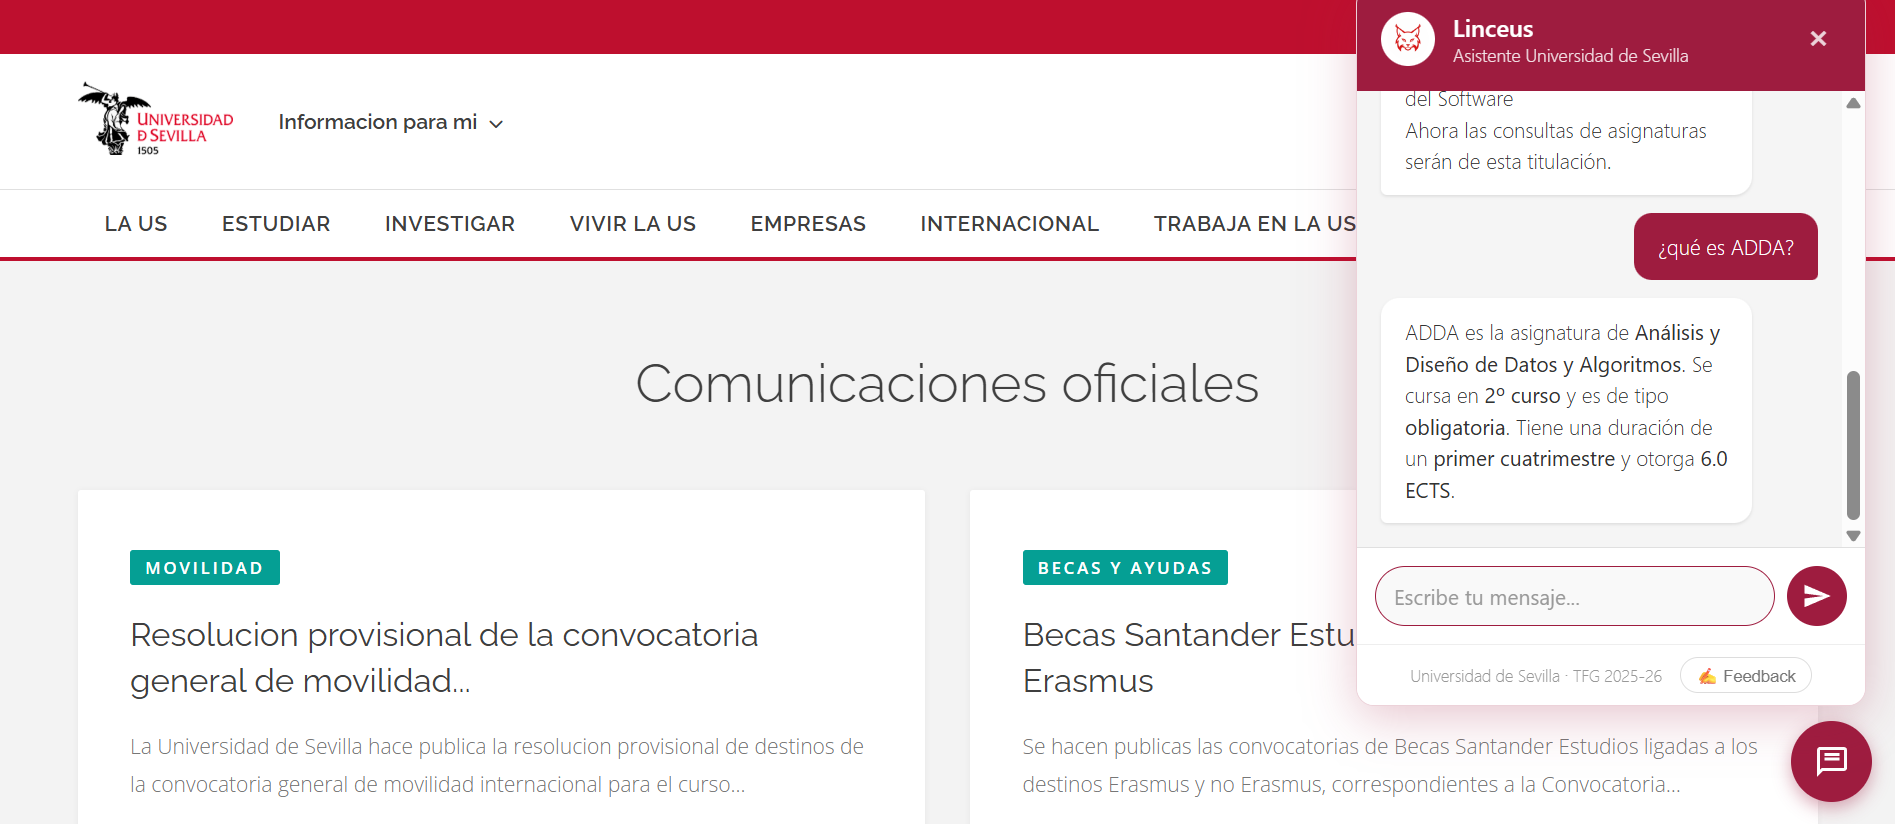
\includegraphics[width=0.95\linewidth]{img/conversacion_ejemplo.png}
\caption{Widget conversacional accesible para el estudiante.}\label{fig:widget-chat}
\end{figure}

\begin{figure}[hbtp]
\centering
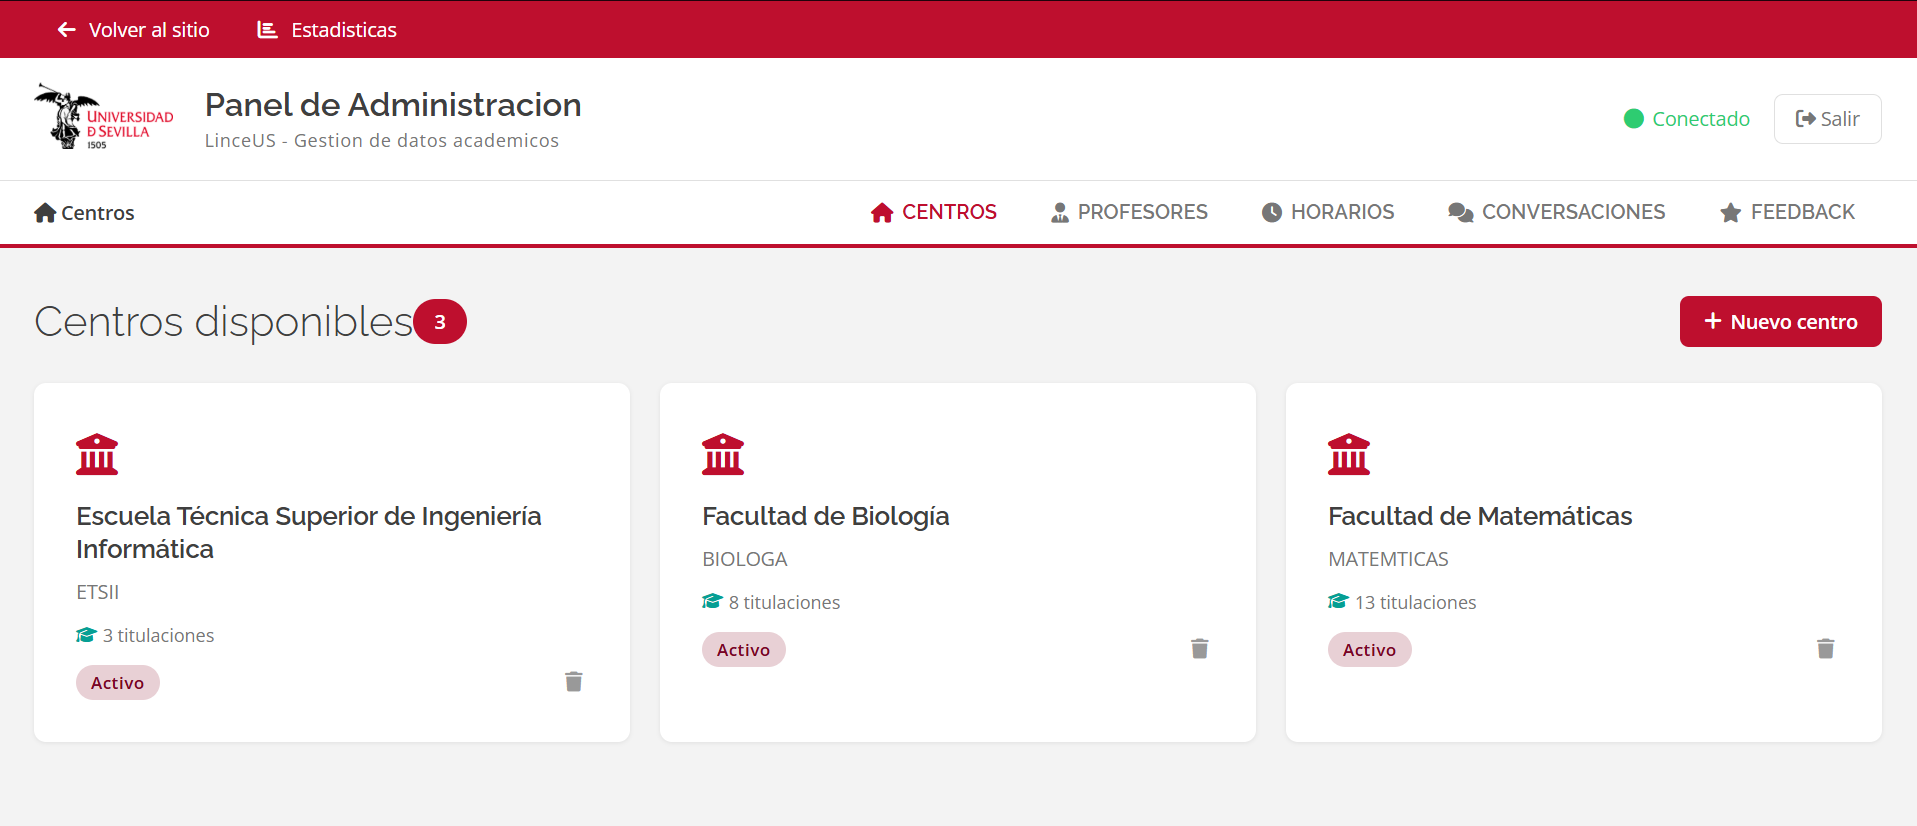
\includegraphics[width=0.95\linewidth]{img/admin_home.png}
\caption{Panel de administración: gestión de asignaturas.}\label{fig:admin-asignaturas}
\end{figure}

\begin{figure}[hbtp]
\centering
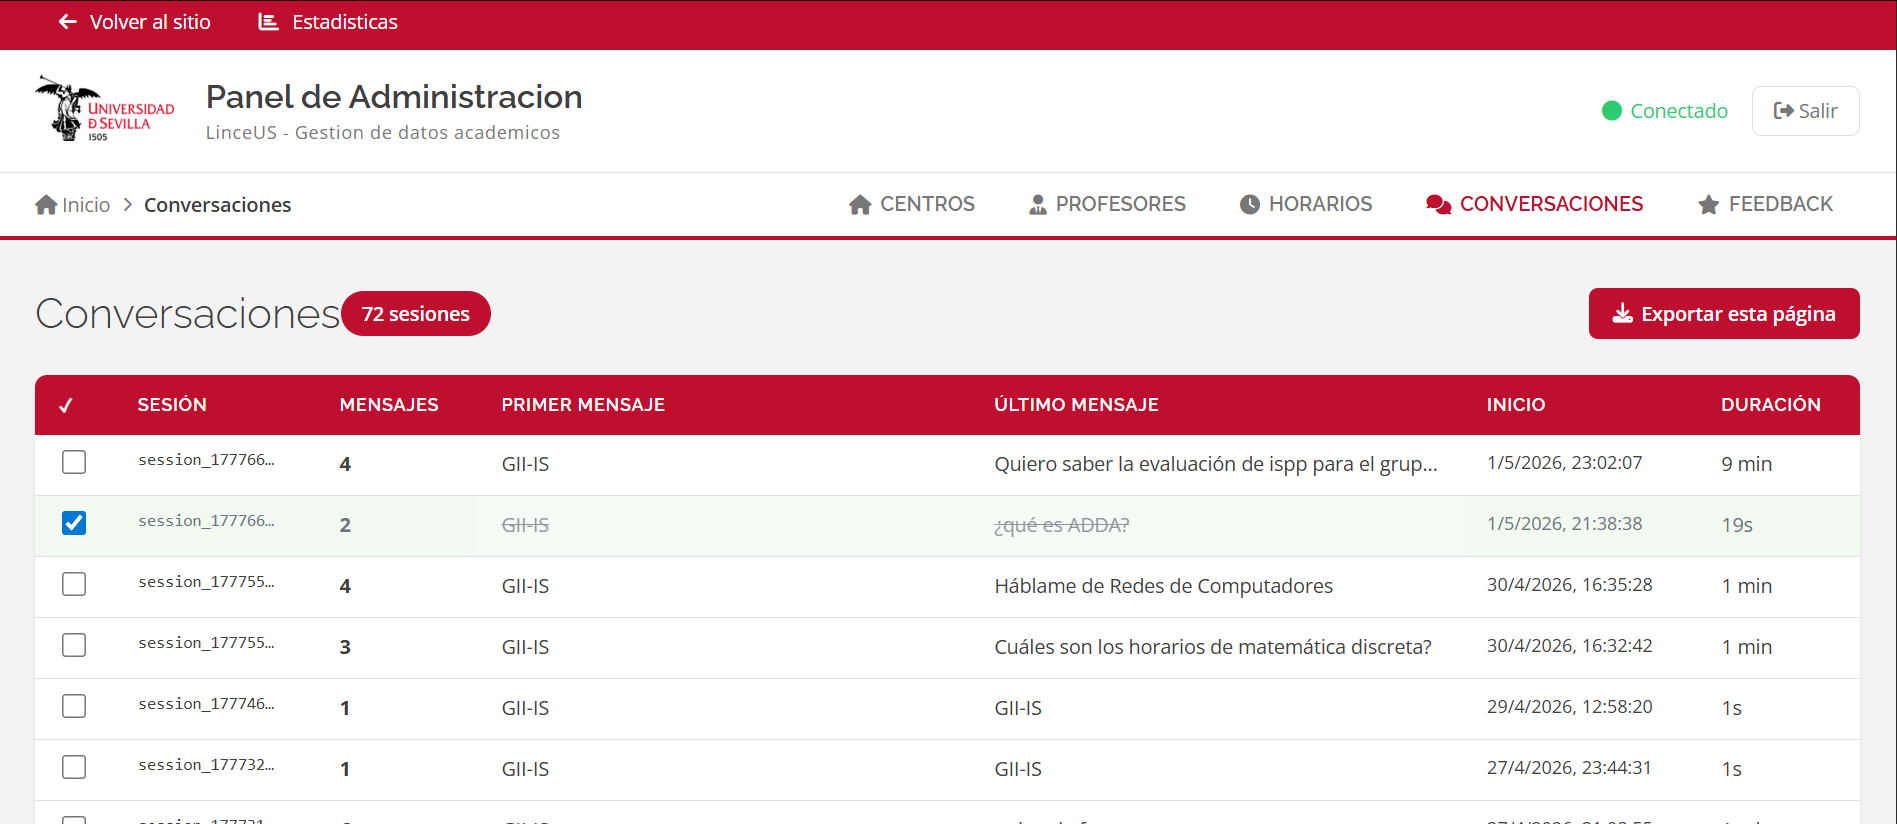
\includegraphics[width=0.95\linewidth]{img/admin_conversaciones.png}
\caption{Panel de administración: auditoría de conversaciones.}\label{fig:admin-conversaciones}
\end{figure}

\begin{figure}[hbtp]
\centering
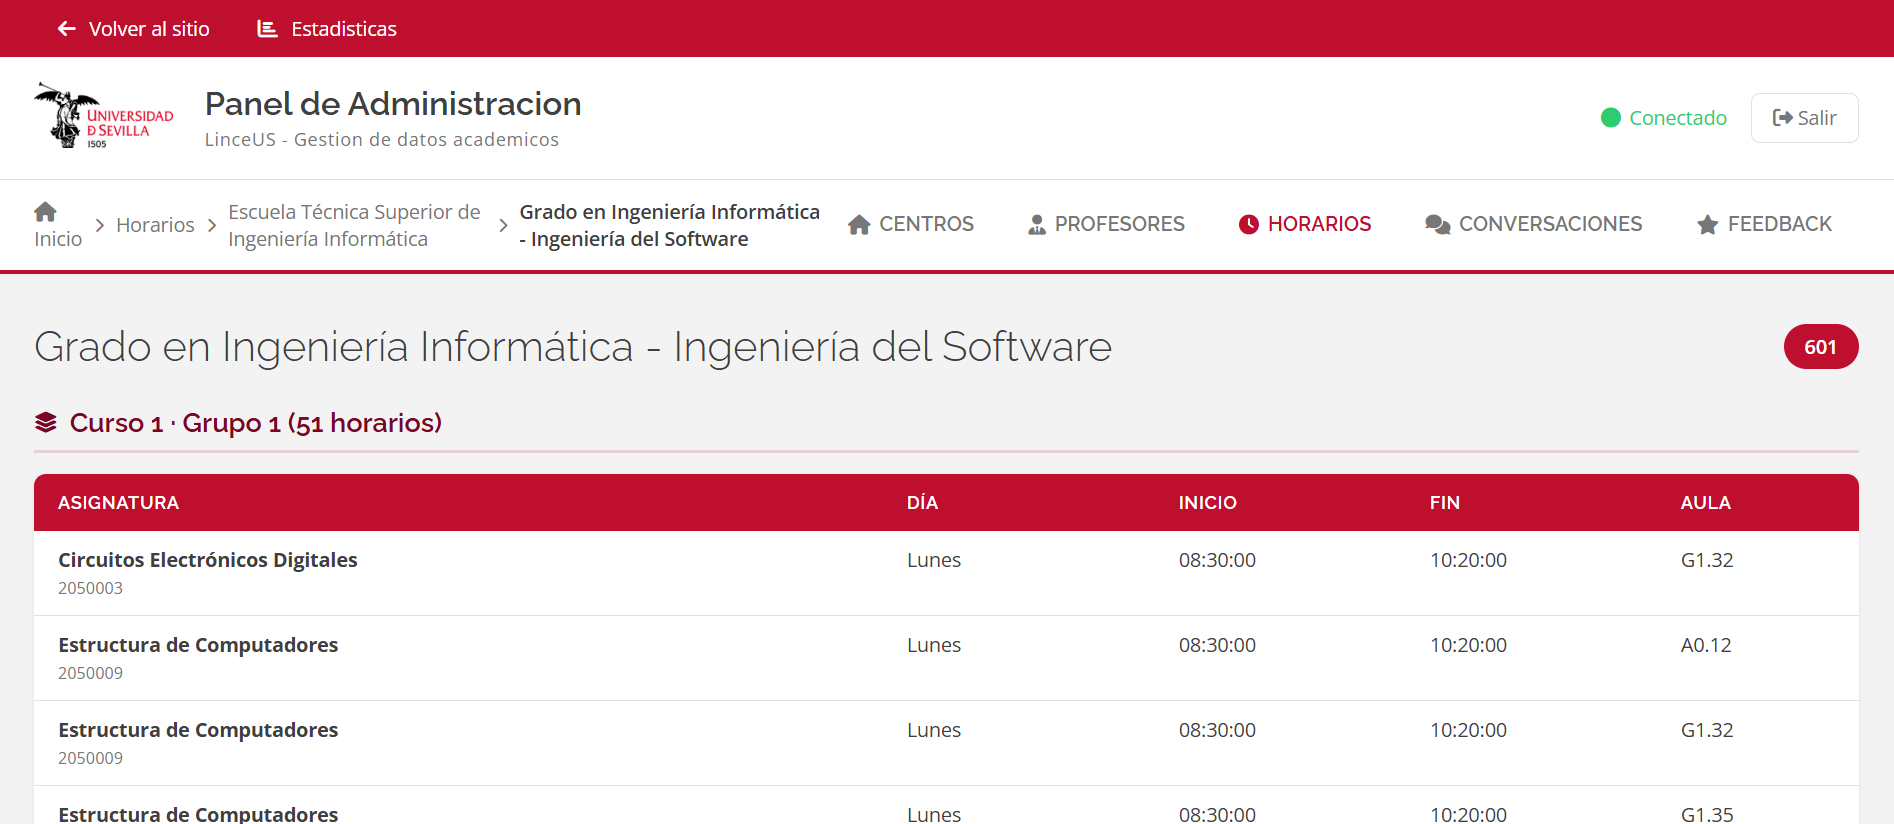
\includegraphics[width=0.95\linewidth]{img/admin_horarios.png}
\caption{Panel de administración: gestión de horarios.}\label{fig:admin-horarios}
\end{figure}

\begin{figure}[hbtp]
\centering
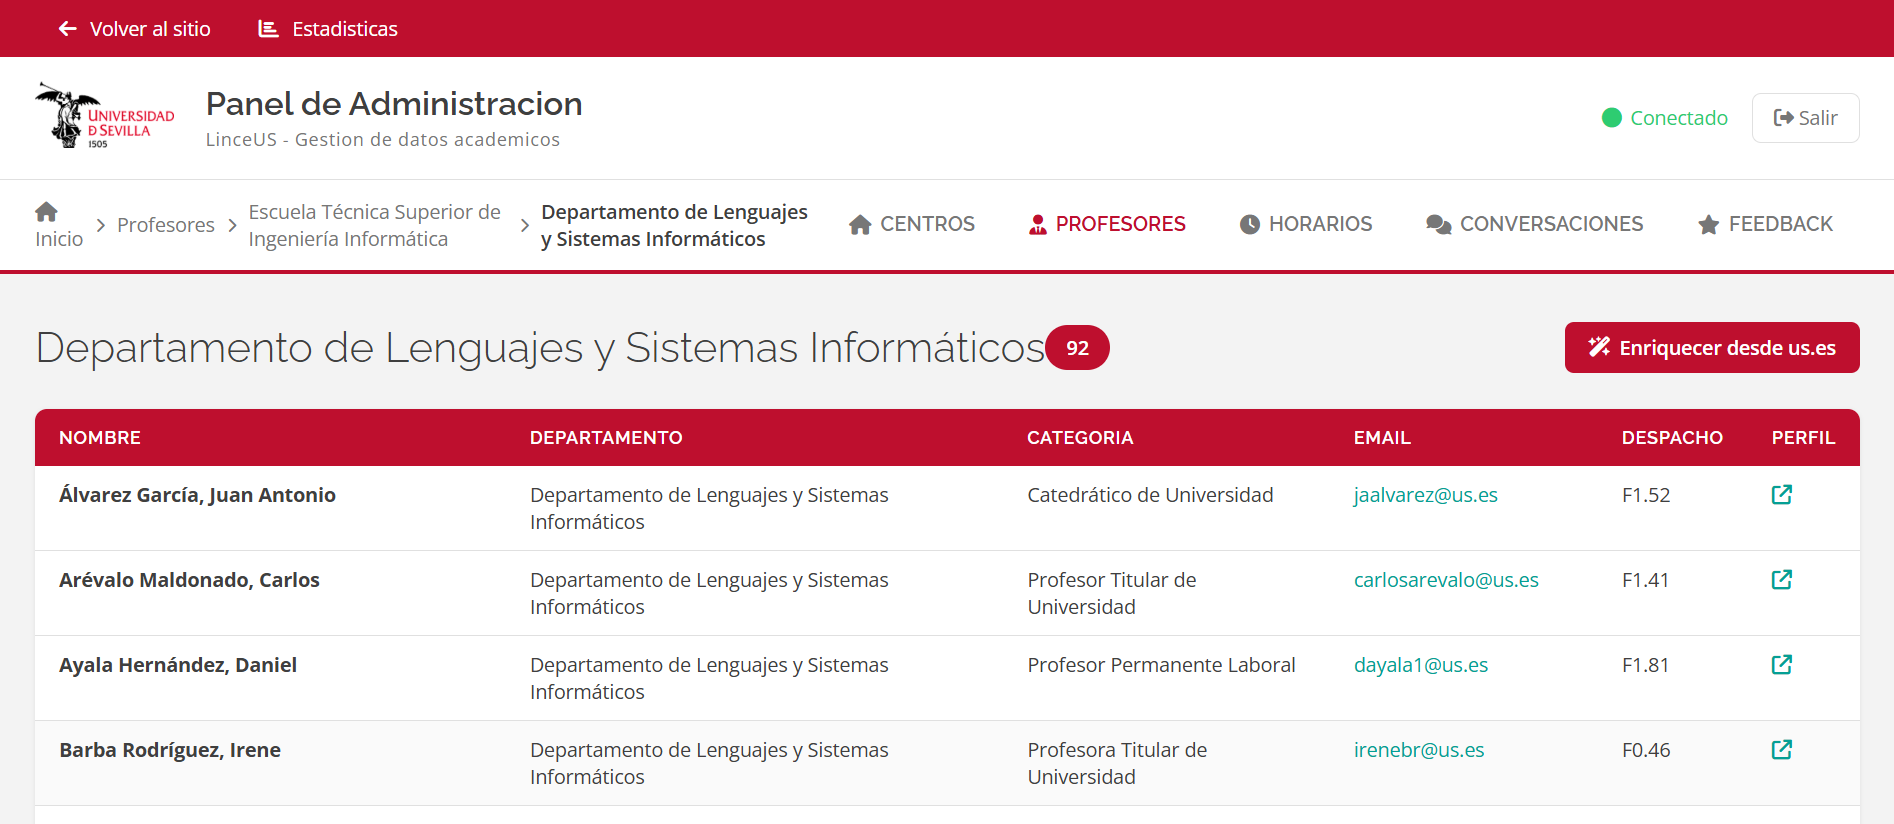
\includegraphics[width=0.95\linewidth]{img/admin_profesores.png}
\caption{Panel de administración: gestión de profesorado.}\label{fig:admin-profesorado}
\end{figure}

\section{Evolución del alcance respecto a la propuesta inicial}\label{sec:req-evolucion}

La propuesta original del proyecto, recogida en el anteproyecto~\cite{segura2024guiatfg}, contemplaba un alcance superior al efectivamente cubierto por el prototipo. La Tabla~\ref{tab:req-evolucion} resume las desviaciones principales y su justificación. En todos los casos las decisiones se han tomado con el objetivo de \textbf{garantizar la calidad de las funcionalidades implementadas}, antes que de cubrir un alcance amplio con calidad insuficiente, en línea con la recomendación de la guía de referencia.

\begin{table}[hbtp]
\centering
\small
\caption{Evolución del alcance respecto a la propuesta inicial.}\label{tab:req-evolucion}
\begin{tabular}{|p{3.0cm}|p{2.0cm}|p{7.5cm}|}
\hline
\textbf{Funcionalidad} & \textbf{Estado} & \textbf{Justificación} \\ \hline
\textit{Frontend} en React & Reformulado & Implementado en HTML/CSS/JavaScript \textit{vanilla} sobre \texttt{nginx}. La inversión de tiempo se ha priorizado en el desarrollo del chatbot, donde el valor añadido del proyecto es mayor. \\ \hline
Notificaciones \textit{push} a estudiantes & Aplazado & Sustituido por el \textbf{panel de administración}, que ofrece mayor valor a la persona que continúe el proyecto y materializa los requisitos de mantenibilidad y escalabilidad. \\ \hline
Soporte multilingüe (inglés) & Aplazado & El corpus académico es mayoritariamente español. Se aplaza a fase 2 cuando el sistema esté estabilizado y exista presupuesto para una segunda suite de pruebas. \\ \hline
Despliegue \textit{on-premise} & Reformulado & La información tratada es de carácter público y la sesión es anónima, por lo que no requiere despliegue en infraestructura propia. Se ha optado por DigitalOcean + Supabase. \\ \hline
Cambio dinámico de titulación & Añadido & Funcionalidad incorporada tras el feedback del piloto (D-029, D-030, D-053). No figuraba en la propuesta inicial. \\ \hline
Integración con \texttt{us.es} para profesorado & Añadido & Sustituye la propuesta inicial de \textit{scrapers} por departamento (D-043, D-044): fuente única, mantenible y completa. \\ \hline
Auditoría manual de conversaciones & Añadido & Surge como necesidad durante la fase de validación; permite la métrica de tráfico real post-despliegue (\S\ref{sec:pruebas-trafico}). \\ \hline
\end{tabular}
\end{table}

El balance final es satisfactorio: el sistema cubre con calidad los tres dominios académicos centrales de la propuesta y aporta dos funcionalidades no previstas (panel de administración y cambio dinámico de titulación) que refuerzan los requisitos de mantenibilidad y experiencia de usuario. Las funcionalidades aplazadas son recuperables en una segunda iteración sin necesidad de modificar el núcleo del sistema, lo que se discute con detalle en el Capítulo~\ref{cap:conclusiones}.

     % !TEX root = ../proyect.tex

\chapter{Arquitectura del sistema y decisiones de diseño}\label{cap:arquitectura}

Este capítulo describe la arquitectura del sistema LinceUS Assistant, las decisiones de diseño adoptadas durante su desarrollo y los diagramas técnicos que representan la estructura de componentes y el modelo de despliegue. El objetivo es ofrecer una visión completa de cómo se organiza internamente el sistema, cómo se comunican sus partes y qué criterios han guiado las principales elecciones técnicas.

% =====================================================
% SECCIÓN 1: ARQUITECTURA GENERAL
% =====================================================

\section{Arquitectura general}\label{sec:arq-general}

LinceUS Assistant sigue una \textbf{arquitectura por capas} (\textit{layered architecture}) con tres niveles claramente diferenciados: capa de presentación, capa de procesamiento conversacional y capa de datos. Esta separación permite que cada capa evolucione de forma independiente y que los cambios en una no afecten directamente a las demás, siempre que se respeten las interfaces definidas entre ellas.

\subsection{Capa de presentación}\label{subsec:capa-presentacion}

La capa de presentación es la interfaz visible para el usuario final. Consiste en un \textbf{widget de chat web} desarrollado en JavaScript puro (vanilla JS), HTML y CSS, diseñado como un componente autocontenido y embebible en cualquier página institucional de la Universidad de Sevilla.

Las principales características de esta capa son:

\begin{itemize}
    \item \textbf{Independencia tecnológica}: El widget no depende de frameworks como React o Angular; se implementa con JavaScript estándar (ES6+), lo que minimiza las dependencias y facilita su integración en páginas web existentes mediante una única etiqueta \texttt{<script>}.
    \item \textbf{Comunicación REST}: El widget se comunica con el servidor Rasa mediante peticiones HTTP POST al endpoint \texttt{/webhooks/rest/webhook}, enviando mensajes del usuario y recibiendo las respuestas del asistente en formato JSON.
    \item \textbf{Renderizado enriquecido}: Soporta formato Markdown en las respuestas del bot, incluyendo tablas, enlaces y listas, para presentar la información académica de forma clara y estructurada.
    \item \textbf{Diseño institucional}: Emplea la identidad visual de la Universidad de Sevilla (colores corporativos, logotipo) para integrarse visualmente en el entorno universitario.
\end{itemize}

\subsection{Capa de procesamiento conversacional}\label{subsec:capa-procesamiento}

Esta capa constituye el núcleo del sistema y está compuesta por varios servicios que colaboran entre sí:

\begin{itemize}
    \item \textbf{Rasa Server}: Motor principal de comprensión del lenguaje natural (NLU) y gestión de diálogo (Core). Recibe los mensajes del usuario, los procesa a través del pipeline NLU para extraer intenciones y entidades, y decide la siguiente acción a ejecutar mediante las políticas de diálogo configuradas.
    \item \textbf{Action Server (Rasa SDK)}: Servidor independiente que ejecuta las acciones personalizadas escritas en Python. Cuando Rasa Core determina que debe ejecutarse una acción personalizada (por ejemplo, consultar la base de datos), delega la ejecución en este servidor a través de una petición HTTP al endpoint \texttt{/webhook}.
    \item \textbf{Google Gemini API}: Servicio externo utilizado para dos propósitos: (1) generación de consultas SQL a partir de lenguaje natural (\textit{Text-to-SQL}) mediante el modelo \texttt{gemma-3-27b-it}, y (2) generación de embeddings vectoriales mediante el modelo \texttt{gemini-embedding-001} para la búsqueda semántica en el pipeline RAG.
    \item \textbf{Ollama} (opcional): Servicio local de inferencia de modelos LLM que actúa como alternativa a Gemini cuando la API externa no está disponible o se agotan las cuotas de uso. Permite ejecutar modelos como \texttt{llama3.2:3b} en CPU sin depender de servicios en la nube.
\end{itemize}

\subsection{Capa de datos}\label{subsec:capa-datos}

La capa de datos se implementa sobre \textbf{Supabase}, una plataforma que proporciona una instancia gestionada de PostgreSQL con extensiones adicionales:

\begin{itemize}
    \item \textbf{PostgreSQL}: Almacena toda la información académica estructurada: universidades, centros, titulaciones, asignaturas, planes docentes y sus metadatos asociados.
    \item \textbf{pgvector}: Extensión que añade el tipo de dato \texttt{vector} y operadores de similitud (distancia coseno, euclidiana y producto punto). Almacena los embeddings de los fragmentos de documentos vectorizados y permite realizar búsquedas semánticas eficientes mediante índices HNSW.
    \item \textbf{Funciones SQL personalizadas}: Funciones almacenadas en la base de datos que encapsulan la lógica de búsqueda vectorial (\texttt{buscar\_plan\_docente()}, \texttt{buscar\_plan\_docente\_global()}), permitiendo filtrar por asignatura, grupo y curso académico con un umbral de similitud configurable.
\end{itemize}

% =====================================================
% SECCIÓN 2: DIAGRAMA DE COMPONENTES
% =====================================================

\section{Diagrama de componentes}\label{sec:diagrama-componentes}

El diagrama de componentes muestra los módulos principales del sistema, sus responsabilidades y las interfaces a través de las cuales se comunican. La Figura~\ref{fig:componentes} representa esta vista.

\begin{figure}[hbtp]
\centering
\resizebox{\textwidth}{!}{%
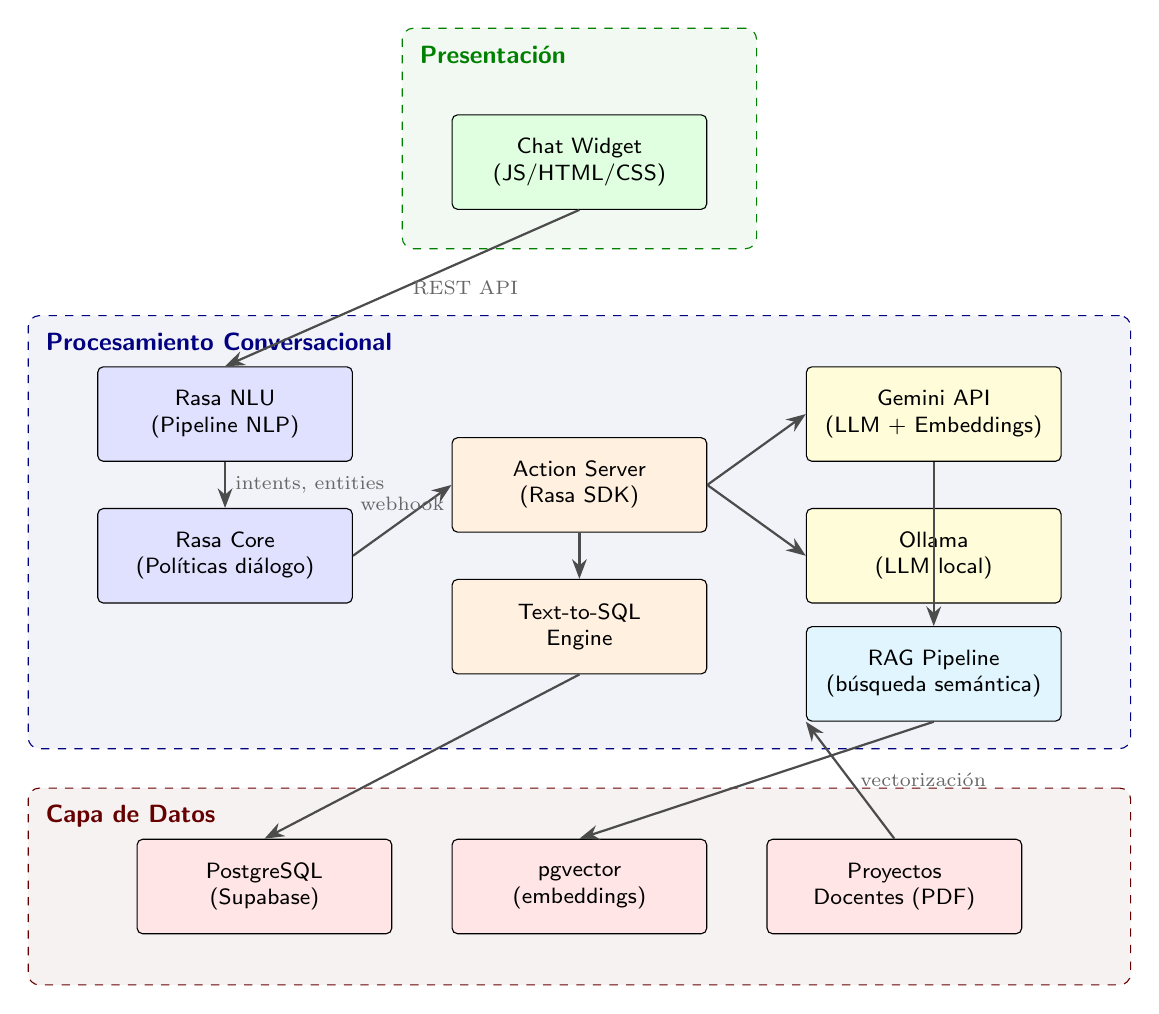
\begin{tikzpicture}[
    component/.style={rectangle, draw=black, fill=#1, minimum width=3.2cm, minimum height=1.2cm, text width=3cm, align=center, font=\footnotesize\sffamily, rounded corners=2pt},
    component/.default={blue!8},
    layer/.style={rectangle, draw=#1, fill=#1!5, dashed, rounded corners=4pt, inner sep=10pt},
    layer/.default={gray!60},
    arrow/.style={-{Stealth[length=2.5mm]}, thick, #1},
    arrow/.default={black!70},
    label/.style={font=\small\sffamily\bfseries, #1},
    label/.default={black}
]

% === CAPA DE PRESENTACIÓN ===
\node[layer=green!50!black, minimum width=4.5cm, minimum height=2.8cm] (pres) at (0, 0) {};
\node[label=green!50!black, anchor=north west] at ([xshift=3pt, yshift=-3pt] pres.north west) {Presentación};
\node[component=green!12] (widget) at (0, -0.3) {Chat Widget\\(JS/HTML/CSS)};

% === CAPA DE PROCESAMIENTO ===
\node[layer=blue!50!black, minimum width=14cm, minimum height=5.5cm] (proc) at (0, -5) {};
\node[label=blue!50!black, anchor=north west] at ([xshift=3pt, yshift=-3pt] proc.north west) {Procesamiento Conversacional};

\node[component=blue!12] (nlu) at (-4.5, -3.5) {Rasa NLU\\(Pipeline NLP)};
\node[component=blue!12] (core) at (-4.5, -5.3) {Rasa Core\\(Políticas diálogo)};
\node[component=orange!12] (actions) at (0, -4.4) {Action Server\\(Rasa SDK)};
\node[component=orange!12] (txtsql) at (0, -6.2) {Text-to-SQL\\Engine};
\node[component=yellow!15] (gemini) at (4.5, -3.5) {Gemini API\\(LLM + Embeddings)};
\node[component=yellow!15] (ollama) at (4.5, -5.3) {Ollama\\(LLM local)};
\node[component=cyan!12] (rag) at (4.5, -6.8) {RAG Pipeline\\(búsqueda semántica)};

% === CAPA DE DATOS ===
\node[layer=red!40!black, minimum width=14cm, minimum height=2.5cm] (data) at (0, -9.5) {};
\node[label=red!40!black, anchor=north west] at ([xshift=3pt, yshift=-3pt] data.north west) {Capa de Datos};

\node[component=red!10] (pg) at (-4, -9.5) {PostgreSQL\\(Supabase)};
\node[component=red!10] (pgvec) at (0, -9.5) {pgvector\\(embeddings)};
\node[component=red!10] (docs) at (4, -9.5) {Proyectos\\Docentes (PDF)};

% === FLECHAS ===
% Presentación → Procesamiento
\draw[arrow] (widget.south) -- node[right, font=\scriptsize, text=black!60] {REST API} (nlu.north);

% Dentro de procesamiento
\draw[arrow] (nlu.south) -- node[right, font=\scriptsize, text=black!60] {intents, entities} (core.north);
\draw[arrow] (core.east) -- node[above, font=\scriptsize, text=black!60] {webhook} (actions.west);
\draw[arrow] (actions.south) -- (txtsql.north);
\draw[arrow] (actions.east) -- (gemini.west);
\draw[arrow] (actions.east) -- (ollama.west);
\draw[arrow] (gemini.south) -- (rag.north);

% Procesamiento → Datos
\draw[arrow] (txtsql.south) -- (pg.north);
\draw[arrow] (rag.south) -- (pgvec.north);
\draw[arrow] (docs.north) -- node[right, font=\scriptsize, text=black!60] {vectorización} (rag.south west);

\end{tikzpicture}
}%
\caption{Diagrama de componentes del sistema LinceUS Assistant.}
\label{fig:componentes}
\end{figure}

A continuación se describe la responsabilidad de cada componente y las interfaces entre ellos:

\begin{itemize}
    \item \textbf{Chat Widget $\rightarrow$ Rasa NLU}: El widget envía el texto del usuario mediante una petición HTTP POST al endpoint REST de Rasa. La comunicación es síncrona: el widget espera la respuesta para mostrarla en la interfaz.
    \item \textbf{Rasa NLU $\rightarrow$ Rasa Core}: Tras procesar el mensaje a través del pipeline NLU (tokenización, extracción de características, clasificación de intención y extracción de entidades), el resultado se pasa al módulo Core, que decide la siguiente acción.
    \item \textbf{Rasa Core $\rightarrow$ Action Server}: Cuando la acción seleccionada es personalizada (prefijo \texttt{action\_}), Core envía una petición HTTP al Action Server con el tracker completo de la conversación (historial, slots, última intención y entidades).
    \item \textbf{Action Server $\rightarrow$ Text-to-SQL}: Para consultas sobre asignaturas, el Action Server invoca el motor Text-to-SQL, que construye un prompt con el esquema de la base de datos y la pregunta del usuario, lo envía a Gemini y recibe una consulta SQL validada.
    \item \textbf{Action Server $\rightarrow$ Gemini / Ollama}: El Action Server puede invocar Gemini para generación de SQL, detección de titulación o generación de embeddings. Si Gemini no está disponible, se recurre a Ollama como alternativa local.
    \item \textbf{RAG Pipeline $\rightarrow$ pgvector}: La búsqueda semántica genera un embedding de la pregunta del usuario y lo compara contra los embeddings almacenados en pgvector usando similitud coseno, con un umbral mínimo de 0.5.
    \item \textbf{Text-to-SQL $\rightarrow$ PostgreSQL}: Las consultas SQL generadas se ejecutan directamente contra la base de datos PostgreSQL de Supabase, con filtros de seguridad inyectados automáticamente (restricción por titulación).
\end{itemize}

% =====================================================
% SECCIÓN 3: DIAGRAMA DE DESPLIEGUE
% =====================================================

\section{Diagrama de despliegue}\label{sec:diagrama-despliegue}

El diagrama de despliegue describe la distribución física de los componentes del sistema en nodos de ejecución y las conexiones de red entre ellos. La Figura~\ref{fig:despliegue} muestra esta configuración.

\begin{figure}[hbtp]
\centering
\resizebox{\textwidth}{!}{%
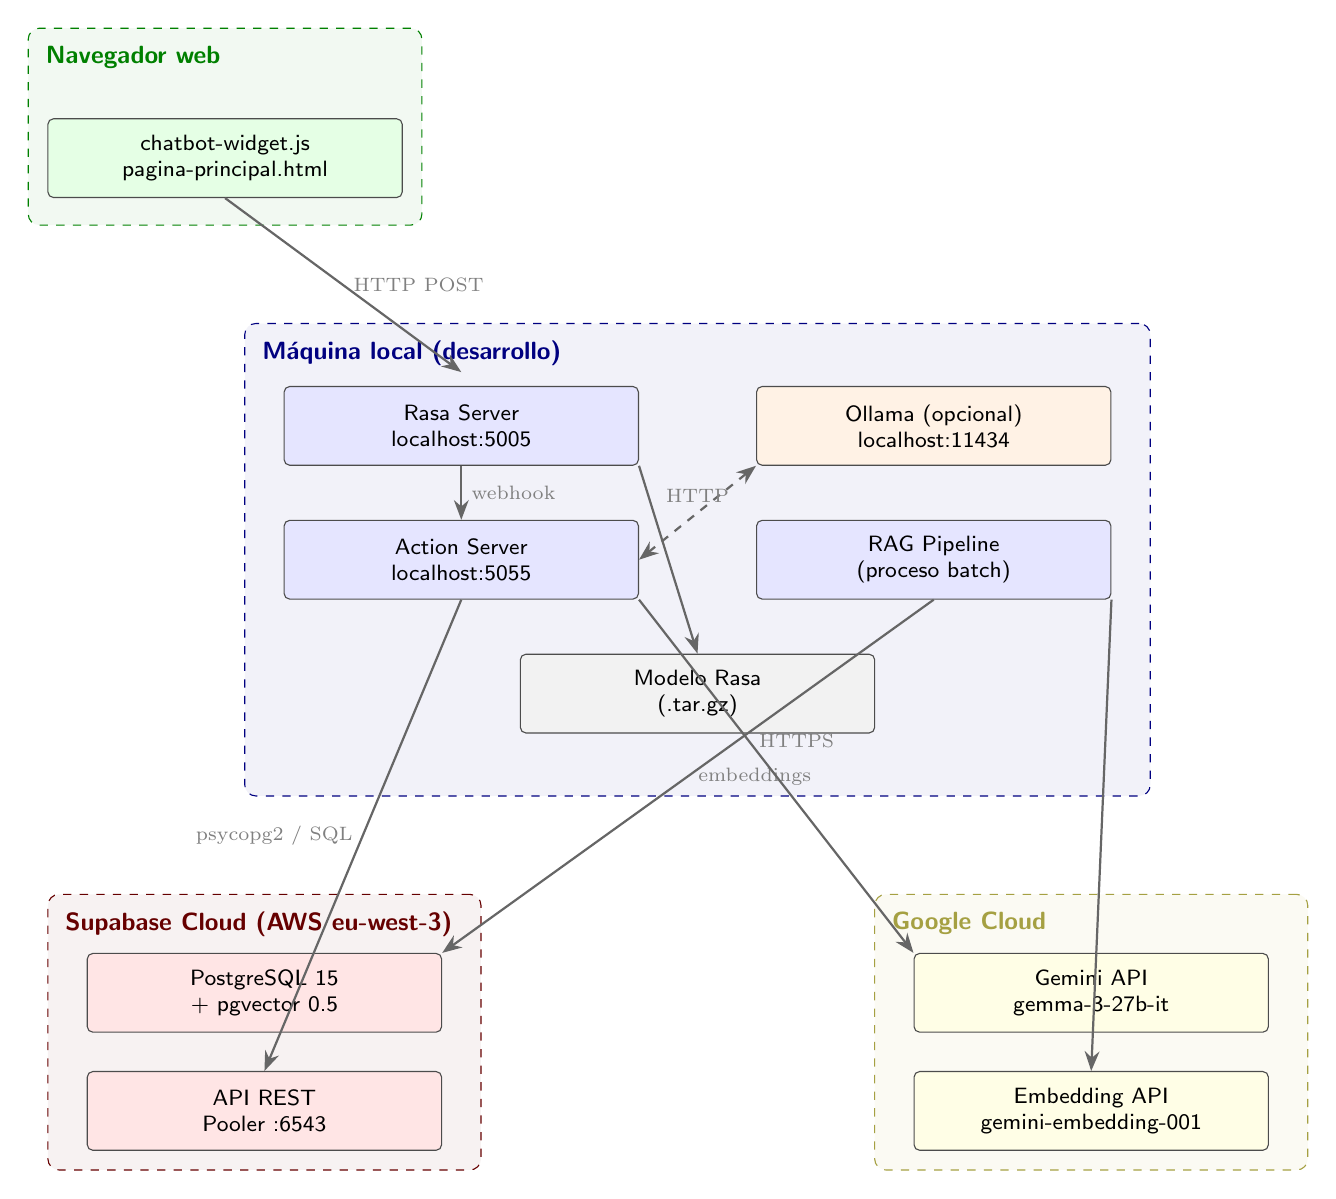
\begin{tikzpicture}[
    node/.style={rectangle, draw=black!70, fill=#1, minimum width=4.5cm, minimum height=1cm, text width=4.2cm, align=center, font=\footnotesize\sffamily, rounded corners=2pt},
    node/.default={white},
    host/.style={rectangle, draw=#1, fill=#1!5, rounded corners=4pt, inner sep=12pt, dashed},
    host/.default={gray!60},
    hlabel/.style={font=\small\sffamily\bfseries, #1},
    hlabel/.default={black},
    conn/.style={-{Stealth[length=2.5mm]}, thick, #1},
    conn/.default={black!60},
    biconn/.style={{Stealth[length=2.5mm]}-{Stealth[length=2.5mm]}, thick, #1},
    biconn/.default={black!60}
]

% === NODO: NAVEGADOR ===
\node[host=green!50!black, minimum width=5cm, minimum height=2.5cm] (browser) at (-6, 0) {};
\node[hlabel=green!50!black, anchor=north west] at ([xshift=3pt, yshift=-3pt] browser.north west) {Navegador web};
\node[node=green!10] (wid) at (-6, -0.4) {chatbot-widget.js\\pagina-principal.html};

% === NODO: MÁQUINA LOCAL ===
\node[host=blue!50!black, minimum width=11.5cm, minimum height=6cm] (local) at (0, -5.5) {};
\node[hlabel=blue!50!black, anchor=north west] at ([xshift=3pt, yshift=-3pt] local.north west) {Máquina local (desarrollo)};

\node[node=blue!10] (rasa) at (-3, -3.8) {Rasa Server\\localhost:5005};
\node[node=blue!10] (actserv) at (-3, -5.5) {Action Server\\localhost:5055};
\node[node=orange!10] (ollamanode) at (3, -3.8) {Ollama (opcional)\\localhost:11434};
\node[node=blue!10] (ragpipe) at (3, -5.5) {RAG Pipeline\\(proceso batch)};
\node[node=gray!10] (model) at (0, -7.2) {Modelo Rasa\\(.tar.gz)};

% === NODO: SUPABASE CLOUD ===
\node[host=red!40!black, minimum width=5.5cm, minimum height=3.5cm] (supa) at (-5.5, -11.5) {};
\node[hlabel=red!40!black, anchor=north west] at ([xshift=3pt, yshift=-3pt] supa.north west) {Supabase Cloud (AWS eu-west-3)};
\node[node=red!10] (pgnode) at (-5.5, -11) {PostgreSQL 15\\+ pgvector 0.5};
\node[node=red!10] (apirest) at (-5.5, -12.5) {API REST\\Pooler :6543};

% === NODO: GOOGLE CLOUD ===
\node[host=yellow!60!black, minimum width=5.5cm, minimum height=3.5cm] (gcloud) at (5, -11.5) {};
\node[hlabel=yellow!60!black, anchor=north west] at ([xshift=3pt, yshift=-3pt] gcloud.north west) {Google Cloud};
\node[node=yellow!10] (gemnode) at (5, -11) {Gemini API\\gemma-3-27b-it};
\node[node=yellow!10] (embnode) at (5, -12.5) {Embedding API\\gemini-embedding-001};

% === CONEXIONES ===
\draw[conn] (wid.south) -- node[right, font=\scriptsize, text=black!50] {HTTP POST} ([yshift=5pt] rasa.north);
\draw[conn] (rasa.south) -- node[right, font=\scriptsize, text=black!50] {webhook} (actserv.north);
\draw[biconn, dashed] (actserv.east) -- node[above, font=\scriptsize, text=black!50] {HTTP} (ollamanode.south west);
\draw[conn] (rasa.south east) -- node[right, font=\scriptsize, text=black!50] {} (model.north);

\draw[conn] (actserv.south) -- node[left, font=\scriptsize, text=black!50] {psycopg2 / SQL} (apirest.north);
\draw[conn] (ragpipe.south) -- node[right, font=\scriptsize, text=black!50] {embeddings} (pgnode.north east);
\draw[conn] (actserv.south east) -- node[right, font=\scriptsize, text=black!50, pos=0.4] {HTTPS} (gemnode.north west);
\draw[conn] (ragpipe.south east) -- node[right, font=\scriptsize, text=black!50] {} (embnode.north);

\end{tikzpicture}
}%
\caption{Diagrama de despliegue del sistema LinceUS Assistant.}
\label{fig:despliegue}
\end{figure}

\subsection{Nodos de ejecución}

El sistema se despliega sobre los siguientes nodos:

\begin{enumerate}
    \item \textbf{Navegador web del usuario}: Ejecuta el widget de chat (JavaScript) y se comunica con el servidor Rasa mediante HTTP. No requiere instalación alguna por parte del usuario.

    \item \textbf{Máquina local de desarrollo}: Alberga los tres servicios principales del backend:
    \begin{itemize}
        \item \textit{Rasa Server} (\texttt{localhost:5005}): Sirve la API REST del chatbot y carga el modelo entrenado (\texttt{.tar.gz}).
        \item \textit{Action Server} (\texttt{localhost:5055}): Ejecuta las acciones personalizadas con un timeout de 300 segundos para acomodar consultas LLM en CPU.
        \item \textit{Ollama} (\texttt{localhost:11434}): Servicio opcional de inferencia local de modelos LLM.
        \item \textit{RAG Pipeline}: Proceso batch que se ejecuta bajo demanda para vectorizar nuevos documentos PDF.
    \end{itemize}

    \item \textbf{Supabase Cloud (AWS eu-west-3)}: Instancia gestionada de PostgreSQL con pgvector, accesible mediante connection pooling en el puerto 6543. Aloja tanto los datos estructurados como los embeddings vectoriales.

    \item \textbf{Google Cloud}: Proporciona acceso a la API de Gemini para generación de texto (Text-to-SQL) y generación de embeddings. La comunicación se realiza mediante HTTPS con autenticación por API key.
\end{enumerate}

\subsection{Protocolos de comunicación}

\begin{table}[hbtp]
\centering
\begin{tabular}{|l|l|l|l|}
\hline
\textbf{Origen} & \textbf{Destino} & \textbf{Protocolo} & \textbf{Puerto} \\ \hline
Navegador & Rasa Server & HTTP POST (REST) & 5005 \\ \hline
Rasa Server & Action Server & HTTP POST (webhook) & 5055 \\ \hline
Action Server & Supabase & TCP (psycopg2) & 6543 \\ \hline
Action Server & Gemini API & HTTPS (REST) & 443 \\ \hline
Action Server & Ollama & HTTP (REST) & 11434 \\ \hline
RAG Pipeline & Supabase & TCP (psycopg2) & 6543 \\ \hline
RAG Pipeline & Gemini Embeddings & HTTPS (REST) & 443 \\ \hline
\end{tabular}
\caption{Protocolos y puertos de comunicación entre nodos del sistema.}
\label{tab:protocolos}
\end{table}

% =====================================================
% SECCIÓN 4: DECISIONES DE DISEÑO
% =====================================================

\section{Decisiones de diseño}\label{sec:decisiones-diseno}

A lo largo del desarrollo del sistema se han tomado decisiones de diseño que han condicionado la arquitectura, el rendimiento y la mantenibilidad del proyecto. En esta sección se documentan las más relevantes, indicando el contexto, las alternativas consideradas y la justificación de cada elección.

\subsection{Text-to-SQL con LLM en lugar de reglas estáticas}\label{subsec:dd-texttosql}

\textbf{Contexto:} El sistema debe responder consultas sobre asignaturas que pueden formularse de formas muy diversas (por nombre, curso, tipología, créditos, duración o combinaciones de estos filtros). Implementar todas las variantes mediante reglas \textit{if-else} o expresiones regulares resultaría en un código excesivamente largo, frágil y difícil de mantener.

\textbf{Decisión:} Se optó por un enfoque \textbf{Text-to-SQL basado en LLM}, donde el modelo Gemini (\texttt{gemma-3-27b-it}) recibe un prompt que incluye el esquema de la tabla \texttt{asignaturas}, las columnas permitidas y la pregunta del usuario, y genera la consulta SQL correspondiente.

\textbf{Justificación:}
\begin{itemize}
    \item \textbf{Flexibilidad}: El modelo interpreta preguntas en lenguaje natural sin necesidad de anticipar todas las formulaciones posibles.
    \item \textbf{Mantenibilidad}: Añadir nuevos atributos o filtros solo requiere actualizar el prompt, no reescribir lógica de parsing.
    \item \textbf{Seguridad}: Se aplican mecanismos de protección como una \textit{whitelist} de columnas permitidas, prohibición de subconsultas e inyección automática del filtro de titulación.
\end{itemize}

\textbf{Temperatura 0.0:} Se configura el modelo con temperatura cero para obtener respuestas deterministas, crítico para la generación de SQL donde la variabilidad es indeseable.

\subsection{Gemini como servicio principal con Ollama como alternativa local}\label{subsec:dd-gemini-ollama}

\textbf{Contexto:} El sistema requiere un modelo de lenguaje grande para Text-to-SQL y generación de embeddings. Depender exclusivamente de una API externa implica riesgos de disponibilidad y costes, mientras que depender solo de ejecución local exige hardware potente.

\textbf{Decisión:} Se adoptó una \textbf{estrategia dual}: Gemini como servicio principal (plan gratuito con 15.000 peticiones/día) y Ollama como alternativa local para situaciones donde la API externa no esté disponible.

\textbf{Justificación:}
\begin{itemize}
    \item El plan gratuito de Gemini es suficiente para el volumen de uso académico del proyecto.
    \item Ollama con \texttt{llama3.2:3b} permite seguir operando sin conexión a internet, aunque con menor calidad en las respuestas.
    \item Esta dualidad alinea el proyecto con los requisitos de privacidad (RGPD), ya que el flujo local no envía datos a terceros.
\end{itemize}

\subsection{Embeddings de 2000 dimensiones con HNSW}\label{subsec:dd-embeddings}

\textbf{Contexto:} El modelo \texttt{gemini-embedding-001} genera embeddings de 3072 dimensiones de forma nativa. Sin embargo, el índice HNSW de pgvector presenta limitaciones de rendimiento y almacenamiento con dimensionalidades muy altas.

\textbf{Decisión:} Se redujo la dimensionalidad de salida a \textbf{2000 dimensiones} mediante el parámetro \texttt{output\_dimensionality} de la API de Gemini.

\textbf{Justificación:}
\begin{itemize}
    \item 2000 dimensiones ofrecen un equilibrio entre la calidad de la representación semántica y la eficiencia del índice HNSW (parámetros $m=16$, $ef\_construction=64$).
    \item Reduce el tamaño de almacenamiento por vector en aproximadamente un 35\%.
    \item Las pruebas empíricas muestran que la pérdida de precisión en la búsqueda semántica es negligible para el corpus de documentos del proyecto (planes docentes de la ETSII).
\end{itemize}

\subsection{Chunking con solapamiento para preservar contexto}\label{subsec:dd-chunking}

\textbf{Contexto:} Los planes docentes en PDF contienen información densa que debe fragmentarse para su vectorización. Un chunking demasiado grande diluye la relevancia; uno demasiado pequeño pierde contexto.

\textbf{Decisión:} Se implementó un chunking de \textbf{800 caracteres con 100 caracteres de solapamiento} y un mínimo de 50 caracteres por fragmento.

\textbf{Justificación:}
\begin{itemize}
    \item 800 caracteres ($\approx$150--200 tokens) es suficiente para capturar un párrafo o sección temática completa.
    \item El solapamiento de 100 caracteres garantiza que la información en los límites de fragmentos no se pierda, preservando la coherencia semántica.
    \item Se aplica detección de secciones por expresiones regulares (``Datos básicos'', ``Objetivos'', ``Contenidos'', ``Evaluación'', ``Bibliografía'') para etiquetar cada fragmento con su sección de origen.
\end{itemize}

\subsection{Búsqueda vectorial con fallback a búsqueda por palabras clave}\label{subsec:dd-fallback}

\textbf{Contexto:} La generación de embeddings para las consultas de búsqueda depende de la API de Gemini, que puede agotar su cuota diaria (100 peticiones por minuto, 1000 por día).

\textbf{Decisión:} Se implementó un sistema de \textbf{doble búsqueda}: búsqueda vectorial como método principal y búsqueda por palabras clave (\texttt{ILIKE}) como fallback automático.

\textbf{Justificación:}
\begin{itemize}
    \item La búsqueda vectorial ofrece mejor precisión semántica (encuentra ``sistema de evaluación'' cuando el usuario pregunta ``¿cómo se califica?'').
    \item El fallback por palabras clave garantiza que el sistema siga operativo aunque la API de embeddings no esté disponible, con resultados razonables para consultas que contienen términos exactos.
    \item El umbral de similitud coseno se fija en 0.5, bajo el cual los resultados se descartan por considerarse irrelevantes.
\end{itemize}

\subsection{Fuzzy matching para resolución de nombres}\label{subsec:dd-fuzzy}

\textbf{Contexto:} Los usuarios introducen nombres de asignaturas con errores ortográficos, sin tildes, con abreviaturas o con variaciones coloquiales (``FP'' por ``Fundamentos de Programación'', ``ADDA'' por ``Análisis y Diseño de Datos y Algoritmos'').

\textbf{Decisión:} Se integró la librería \textbf{RapidFuzz} con un umbral de similitud del 80\% combinado con una tabla de alias y acrónimos mantenida en el código.

\textbf{Justificación:}
\begin{itemize}
    \item El algoritmo de distancia de Levenshtein de RapidFuzz tolera errores tipográficos habituales sin requerir entrenamiento adicional.
    \item La tabla de alias cubre las abreviaturas más comunes utilizadas por los estudiantes de la ETSII.
    \item Si la coincidencia difusa falla, se recurre al LLM (Gemini) como último recurso para intentar identificar la asignatura.
\end{itemize}

\subsection{Slots conversacionales para memoria de contexto}\label{subsec:dd-slots}

\textbf{Contexto:} Los usuarios formulan preguntas de seguimiento que hacen referencia implícita a asignaturas o titulaciones mencionadas previamente (``¿Y cuántos créditos tiene?'', ``¿Es obligatoria?'').

\textbf{Decisión:} Se utilizan \textbf{slots de Rasa} para mantener el estado de la conversación:
\begin{itemize}
    \item \texttt{contexto\_titulacion}: Titulación activa seleccionada por el usuario.
    \item \texttt{ultimo\_codigo\_consultado}: Código de la última asignatura consultada.
    \item \texttt{ultimo\_nombre\_asignatura}: Nombre de la última asignatura mencionada.
    \item \texttt{ultimos\_resultados\_asignaturas}: Lista de resultados de la última consulta (para paginación).
\end{itemize}

\textbf{Justificación:}
\begin{itemize}
    \item Los slots permiten que las acciones personalizadas recuperen el contexto sin que el usuario deba repetir información.
    \item La separación entre código y nombre de asignatura facilita tanto las consultas SQL (por código) como las respuestas al usuario (por nombre legible).
    \item La titulación por defecto es GII-IS (Ingeniería del Software), configurable por el usuario mediante la intención \texttt{cambiar\_contexto\_academico}.
\end{itemize}

\subsection{Pipeline NLU de 9 etapas con doble featurización}\label{subsec:dd-pipeline}

\textbf{Contexto:} El pipeline NLU de Rasa debe ser capaz de clasificar correctamente intenciones en español, tolerando errores ortográficos, abreviaturas y variaciones léxicas propias del lenguaje coloquial estudiantil.

\textbf{Decisión:} Se configuró un pipeline de 9 componentes que combina \textbf{featurización a nivel de palabra} (n-gramas 1--2) y \textbf{a nivel de carácter} (n-gramas 1--4):

\begin{enumerate}
    \item \texttt{WhitespaceTokenizer}: Tokenización por espacios en blanco.
    \item \texttt{RegexFeaturizer}: Patrones regex para códigos de asignatura y formatos especiales.
    \item \texttt{LexicalSyntacticFeaturizer}: Características gramaticales del contexto local.
    \item \texttt{CountVectorsFeaturizer} (palabra): N-gramas de palabras (1--2).
    \item \texttt{CountVectorsFeaturizer} (carácter): N-gramas de caracteres (1--4).
    \item \texttt{DIETClassifier}: Clasificador dual de intenciones y entidades (150 épocas, dropout 0.2).
    \item \texttt{EntitySynonymMapper}: Normalización de sinónimos de entidades.
    \item \texttt{ResponseSelector}: Selección de respuestas tipo FAQ.
    \item \texttt{FallbackClassifier}: Detección de baja confianza (umbral 0.7).
\end{enumerate}

\textbf{Justificación:}
\begin{itemize}
    \item La featurización a nivel de carácter es especialmente eficaz para manejar errores ortográficos (``Fundamnetos'' se reconoce por similitud de caracteres con ``Fundamentos'').
    \item El umbral de fallback de 0.7 equilibra la precisión (evitar respuestas incorrectas) con la cobertura (no rechazar demasiadas consultas legítimas).
    \item El \texttt{DIETClassifier} con 150 épocas y dropout de 0.2 proporciona un modelo robusto sin sobreajuste al conjunto de entrenamiento.
\end{itemize}

\subsection{Hash SHA-256 para evitar reprocesamiento de documentos}\label{subsec:dd-hash}

\textbf{Contexto:} El pipeline de vectorización RAG procesa documentos PDF que pueden ser costosos de re-vectorizar (extracción de texto, chunking, generación de embeddings con API de pago por uso).

\textbf{Decisión:} Se almacena un \textbf{hash SHA-256} de cada PDF procesado en la tabla \texttt{planes\_docentes}. Antes de procesar un documento, se compara el hash actual con el almacenado.

\textbf{Justificación:}
\begin{itemize}
    \item Si el hash coincide, el documento no ha cambiado y se omite el reprocesamiento, ahorrando llamadas a la API de embeddings.
    \item Si el hash difiere, se eliminan los fragmentos anteriores y se reprocessa el documento completo, garantizando la consistencia de los datos.
    \item Este mecanismo es especialmente relevante dado el límite de 1000 embeddings por día del plan gratuito de Gemini.
\end{itemize}

% =====================================================
% SECCIÓN 5: PATRONES ARQUITECTÓNICOS
% =====================================================

\section{Patrones arquitectónicos aplicados}\label{sec:patrones}

El diseño del sistema incorpora varios patrones arquitectónicos reconocidos en la ingeniería del software:

\subsection{Arquitectura por capas (\textit{Layered Architecture})}

Como se ha descrito en la Sección~\ref{sec:arq-general}, el sistema se organiza en tres capas con responsabilidades bien definidas. Cada capa solo se comunica con la inmediatamente inferior, lo que reduce el acoplamiento y facilita el reemplazo de componentes (por ejemplo, cambiar el frontend sin afectar la lógica de negocio).

\subsection{Patrón \textit{Action Server} (microservicio de lógica)}

Rasa delega la ejecución de lógica de negocio en un servidor de acciones independiente. Este patrón es similar al patrón \textit{Backend for Frontend} (BFF), donde un servicio intermedio adapta las respuestas de los servicios de datos al formato esperado por el cliente conversacional. La separación permite escalar el Action Server independientemente del motor Rasa.

\subsection{Patrón \textit{Strategy} para clientes LLM}

Los clientes de Gemini (\texttt{gemini\_client.py}) y Ollama (\texttt{ollama\_client.py}) implementan una interfaz similar para la generación de texto. El Action Server puede alternar entre ambos proveedores en función de la disponibilidad, aplicando el patrón \textit{Strategy} para desacoplar la lógica de negocio del proveedor concreto de LLM.

\subsection{Patrón \textit{Pipeline} para procesamiento RAG}

El pipeline de vectorización sigue el patrón \textit{Pipeline} (o \textit{Pipes and Filters}), donde cada etapa transforma los datos y los pasa a la siguiente: extracción de PDF $\rightarrow$ chunking $\rightarrow$ generación de embeddings $\rightarrow$ inserción en base de datos. Cada etapa es independiente y puede modificarse sin afectar a las demás.

\subsection{Patrón \textit{Repository} para acceso a datos}

El módulo \texttt{db.py} centraliza todas las operaciones contra la base de datos, proporcionando una abstracción que oculta los detalles de conexión (pool de conexiones psycopg2) y ejecución de consultas al resto del sistema. Esto facilita el testing unitario mediante mocks y permite cambiar la implementación de persistencia sin modificar la lógica de negocio.

     % !TEX root = ../proyect.tex

\chapter{Marco tecnológico}\label{cap:marco-tecnologico}

Este capítulo describe el conjunto de tecnologías, frameworks y paradigmas que conforman la base técnica del proyecto LinceUS Assistant. Se complementa con el Capítulo~\ref{cap:arquitectura}, donde se detallan la arquitectura del sistema, las decisiones de diseño y los diagramas de componentes y despliegue. Aquí se justifica la elección de cada componente del stack tecnológico.

\section{Tecnologías de procesamiento conversacional}\label{sec:procesamiento-conversacional}

\subsection{Rasa Framework}

Rasa es un framework de código abierto para la construcción de asistentes conversacionales basados en IA. A diferencia de soluciones comerciales como Dialogflow o Lex de AWS, Rasa ofrece:

\begin{itemize}
    \item \textbf{Control total sobre el modelo}: Los datos de entrenamiento y los modelos permanecen bajo control del desarrollador
    \item \textbf{Personalización completa}: Políticas de diálogo y pipelines de NLU totalmente configurables
    \item \textbf{Ejecución local}: No depende de servicios externos para funcionar
    \item \textbf{Multilenguaje}: Soporte nativo para español mediante modelos de spaCy
\end{itemize}

\subsubsection{Componentes de Rasa utilizados}

\textbf{Rasa NLU (Natural Language Understanding)}

Rasa NLU se encarga de interpretar la entrada del usuario y extraer:
\begin{itemize}
    \item \textbf{Intenciones (intents)}: ¿Qué quiere hacer el usuario? (e.g., \texttt{consultar\_horario}, \texttt{buscar\_asignatura})
    \item \textbf{Entidades (entities)}: Información específica mencionada por el usuario (e.g., nombre de asignatura, curso, centro)
\end{itemize}

\textbf{Rasa Core}

Rasa Core gestiona el flujo de conversación mediante:
\begin{itemize}
    \item \textbf{Stories}: Conversaciones de ejemplo que entrenan el modelo de diálogo
    \item \textbf{Rules}: Reglas determinísticas para situaciones específicas
    \item \textbf{Políticas}: Algoritmos de aprendizaje que deciden la siguiente acción del bot
\end{itemize}

\textbf{Rasa Actions}

Las acciones personalizadas permiten al bot ejecutar código Python para:
\begin{itemize}
    \item Consultar la base de datos
    \item Generar respuestas dinámicas
    \item Llamar a APIs externas
    \item Procesar lógica de negocio compleja
\end{itemize}

\subsection{Procesamiento de Lenguaje Natural}

\subsubsection{spaCy}

spaCy proporciona capacidades avanzadas de NLP en español:

\begin{itemize}
    \item \textbf{Tokenización}: Separación del texto en palabras y signos de puntuación
    \item \textbf{Lematización}: Reducción de palabras a su forma base
    \item \textbf{Análisis morfológico}: Identificación de categorías gramaticales
    \item \textbf{Vectores de palabras}: Representaciones numéricas del significado de las palabras
\end{itemize}

El modelo \texttt{es\_core\_news\_md} incluye vocabulario específico del español y ha sido entrenado en corpus de textos en español.

\subsubsection{Coincidencia difusa (Fuzzy Matching)}

La librería RapidFuzz implementa algoritmos de distancia de cadenas que permiten:

\begin{itemize}
    \item Tolerar errores ortográficos (e.g., "Fundamnetos de Programacion")
    \item Reconocer abreviaturas (e.g., "FP" por "Fundamentos de Programación")
    \item Manejar variaciones en la escritura (e.g., mayúsculas, tildes)
\end{itemize}

Se utiliza el algoritmo de \textit{Levenshtein distance} con un umbral de similitud del 80\% para considerar coincidencias válidas.

\section{Tecnologías de Inteligencia Artificial}\label{sec:ia}

\subsection{Ollama y modelos de lenguaje grandes (LLMs)}

Ollama es una plataforma que permite ejecutar modelos de lenguaje de gran tamaño localmente, sin necesidad de conexión a servicios cloud. En LinceUS Assistant se utiliza para dos propósitos principales:

\subsubsection{Text-to-SQL}

El sistema implementa un pipeline de generación de consultas SQL a partir de lenguaje natural:

\begin{enumerate}
    \item El usuario formula una pregunta en lenguaje natural
    \item Ollama (usando un modelo como Llama 3 o Mistral) genera la consulta SQL correspondiente
    \item La consulta se valida y ejecuta contra la base de datos
    \item Los resultados se procesan y formatean para presentarlos al usuario
\end{enumerate}

Este enfoque permite consultas complejas sin necesidad de definir explícitamente todas las posibles preguntas.

\subsubsection{Generación de respuestas contextualizadas}

Para consultas que no se ajustan a patrones predefinidos, el modelo LLM genera respuestas naturales basándose en:

\begin{itemize}
    \item El contexto de la conversación
    \item La información recuperada de la base de datos
    \item El conocimiento previo del modelo
\end{itemize}

\subsection{Embeddings y búsqueda semántica}

Para la recuperación de información de documentos (planes docentes, información de trámites), se utiliza:

\begin{itemize}
    \item \textbf{Modelos de embeddings}: Transforman texto en vectores numéricos que capturan el significado semántico
    \item \textbf{pgvector}: Extensión de PostgreSQL que permite almacenar y buscar vectores eficientemente
    \item \textbf{Búsqueda de similitud}: Encuentra documentos relevantes usando distancia coseno entre vectores
\end{itemize}

Este enfoque implementa un sistema RAG (\textit{Retrieval-Augmented Generation}) que mejora la precisión de las respuestas al combinar búsqueda semántica con generación de lenguaje.

\section{Tecnologías de base de datos}\label{sec:base-datos}

\subsection{PostgreSQL}

PostgreSQL es el sistema de gestión de bases de datos relacional utilizado. Se ha elegido por:

\begin{itemize}
    \item \textbf{Robustez}: Base de datos ACID con alta integridad de datos
    \item \textbf{Extensibilidad}: Soporte para tipos de datos personalizados y extensiones
    \item \textbf{Rendimiento}: Optimización de consultas complejas y soporte para índices avanzados
    \item \textbf{Código abierto}: Sin costes de licencia y comunidad activa
\end{itemize}

\subsection{Supabase}

Supabase proporciona una capa de servicios sobre PostgreSQL:

\begin{itemize}
    \item \textbf{API REST automática}: Generación automática de endpoints para operaciones CRUD
    \item \textbf{Real-time}: Suscripciones a cambios en la base de datos
    \item \textbf{Autenticación}: Sistema de usuarios y permisos integrado
    \item \textbf{Almacenamiento}: Para archivos y documentos
    \item \textbf{Funciones Edge}: Ejecución de código serverless
\end{itemize}

La API REST de Supabase simplifica la integración con el backend de Python, eliminando la necesidad de escribir queries SQL manualmente para operaciones básicas.

\subsection{pgvector}

La extensión pgvector añade capacidades de búsqueda vectorial a PostgreSQL:

\begin{itemize}
    \item Almacenamiento eficiente de vectores de alta dimensionalidad (hasta 16,000 dimensiones)
    \item Índices IVFFlat y HNSW para búsquedas rápidas de vecinos más cercanos
    \item Operadores de similitud (distancia euclidiana, producto punto, similitud coseno)
\end{itemize}

Esto permite implementar búsqueda semántica directamente en la base de datos, sin necesidad de sistemas externos como Pinecone o Weaviate.

\section{Tecnologías de frontend}\label{sec:frontend}

\subsection{Node.js}

El frontend del asistente está desarrollado usando Node.js, que proporciona:

\begin{itemize}
    \item \textbf{JavaScript del lado del servidor}: Mismo lenguaje en frontend y backend de la interfaz
    \item \textbf{NPM}: Gestor de paquetes con millones de librerías disponibles
    \item \textbf{Rendimiento}: Motor V8 de alta velocidad
\end{itemize}

\subsection{Framework web}

Se utiliza un framework minimalista que permite:

\begin{itemize}
    \item Servir la interfaz de chat web
    \item Gestionar la conexión WebSocket con el backend de Rasa
    \item Renderizar mensajes con formato enriquecido (tablas, enlaces, imágenes)
\end{itemize}

\section{Herramientas de desarrollo}\label{sec:herramientas-desarrollo-marco}

\subsection{Control de versiones}

\textbf{Git} es el sistema de control de versiones utilizado, con \textbf{GitHub} como plataforma de hosting. La estructura del repositorio incluye:

\begin{itemize}
    \item \texttt{/actions}: Acciones personalizadas de Rasa
    \item \texttt{/data}: Datos de entrenamiento (intents, stories, rules)
    \item \texttt{/models}: Modelos entrenados de Rasa
    \item \texttt{/frontend}: Código de la interfaz web
    \item \texttt{/docs}: Documentación del proyecto
\end{itemize}

\subsection{Gestión de dependencias}

Las dependencias de Python se gestionan mediante:

\begin{itemize}
    \item \textbf{requirements.txt}: Lista de todas las librerías necesarias con versiones específicas
    \item \textbf{Entorno virtual (venv)}: Aislamiento de dependencias del sistema
\end{itemize}

\subsection{Variables de entorno}

La librería \texttt{python-dotenv} gestiona la configuración mediante archivos \texttt{.env}:

\begin{itemize}
    \item Credenciales de Supabase (URL, API key)
    \item Configuración de Ollama (URL del servidor, modelo a utilizar)
    \item Parámetros de configuración del sistema
\end{itemize}

Esto permite cambiar la configuración sin modificar el código y evita exponer credenciales en el repositorio público.

\section{Consideraciones de seguridad}\label{sec:seguridad}

\subsection{Protección de datos}

\begin{itemize}
    \item \textbf{Credenciales}: Nunca se almacenan en el código, siempre en variables de entorno
    \item \textbf{API keys}: Se utilizan claves específicas con permisos mínimos necesarios
    \item \textbf{Conexiones}: HTTPS para todas las comunicaciones con servicios externos
\end{itemize}

\subsection{Validación de entrada}

\begin{itemize}
    \item Sanitización de consultas SQL para prevenir inyección SQL
    \item Validación de tipos de datos en entradas de usuario
    \item Limitación de longitud de mensajes
\end{itemize}

\subsection{Ejecución local de modelos}

El uso de Ollama para ejecutar modelos localmente aporta beneficios de privacidad:

\begin{itemize}
    \item Las consultas de los usuarios no se envían a servicios externos
    \item No hay dependencia de APIs comerciales que puedan cambiar términos de uso
    \item Control total sobre los datos procesados
\end{itemize}

\section{Stack tecnológico completo}\label{sec:stack-completo}

La siguiente tabla resume todas las tecnologías empleadas en el proyecto:

\begin{table}[h]
\centering
\begin{tabular}{|l|l|l|}
\hline
\textbf{Capa} & \textbf{Tecnología} & \textbf{Versión} \\ \hline
Frontend & Node.js & 18.x \\ \hline
Frontend & HTML/CSS/JavaScript & ES6+ \\ \hline
Backend conversacional & Python & 3.10 \\ \hline
Backend conversacional & Rasa & 3.6.21 \\ \hline
Backend conversacional & Rasa SDK & 3.6.2 \\ \hline
Backend conversacional & spaCy & 3.8.0 \\ \hline
IA y LLMs & Ollama & latest \\ \hline
IA y LLMs & Modelos LLM & Llama 3 / Mistral \\ \hline
Base de datos & PostgreSQL & 15.x \\ \hline
Base de datos & pgvector & 0.5.0 \\ \hline
Plataforma BD & Supabase & cloud \\ \hline
Librerías NLP & RapidFuzz & 3.0.0 \\ \hline
Librerías NLP & python-dotenv & 1.0.0 \\ \hline
Control versiones & Git \& GitHub & 2.x \\ \hline
\end{tabular}
\caption{Stack tecnológico completo del proyecto LinceUS Assistant.}
\label{tab:stack-tecnologico}
\end{table}

     % !TEX root = ../proyect.tex

\chapter{Estructura del proyecto}\label{cap:estructura-proyecto}

Este capítulo describe la organización del repositorio LinceUS Assistant, detallando el propósito de cada directorio y fichero relevante. La estructura ha sido diseñada para separar claramente las responsabilidades entre los distintos módulos del sistema y facilitar el mantenimiento y la escalabilidad del proyecto.

\section{Visión general del repositorio}\label{sec:vision-general}

El repositorio sigue una organización modular en la que cada directorio agrupa elementos con una responsabilidad concreta dentro del sistema. La separación entre la lógica conversacional, los datos de entrenamiento, la capa de acceso a datos, la interfaz de usuario y la documentación responde al principio de separación de responsabilidades (\textit{Separation of Concerns}).

El árbol de directorios principal es el siguiente:

\begin{verbatim}
linceus-assistant/
+-- actions/
|   +-- __init__.py
|   +-- actions.py
|   +-- asignaturas.py
|   +-- config.py
|   +-- contexto.py
|   +-- db.py
|   +-- gemini_client.py
|   +-- ollama_client.py
|   \-- text_to_sql.py
+-- data/
|   +-- nlu/
|   |   +-- asignaturas.yml
|   |   +-- contexto.yml
|   |   \-- general.yml
|   +-- rules.yml
|   \-- stories.yml
+-- docs/
|   +-- sprints/
|   \-- other/
+-- frontend/
|   +-- chatbot-widget.js
|   +-- chatbot-icon.html
|   +-- pagina-principal.html
|   \-- pagina-principal.css
+-- memoria_tfg/
+-- tests/
|   \-- test_stories.yml
+-- config.yml
+-- domain.yml
+-- credentials.yml
+-- endpoints.yml
\-- requirements.txt
\end{verbatim}

\section{Directorio raíz}\label{sec:directorio-raiz}

Los ficheros situados en la raíz del repositorio configuran el comportamiento global del sistema Rasa y la gestión de dependencias del proyecto.

\begin{itemize}
    \item \texttt{config.yml}: Define el pipeline de procesamiento de lenguaje natural (NLU) y las políticas de diálogo de Rasa. Especifica los componentes utilizados para tokenización, extracción de características e identificación de intenciones y entidades.
    \item \texttt{domain.yml}: Declara el universo del asistente: intenciones, entidades, slots, acciones y respuestas predefinidas. Es el fichero central que Rasa utiliza para construir el modelo de diálogo.
    \item \texttt{credentials.yml}: Contiene las credenciales de conexión con los canales de comunicación externos (REST, Slack, etc.). Las claves sensibles se gestionan mediante variables de entorno para no exponerlas en el repositorio.
    \item \texttt{endpoints.yml}: Configura los endpoints de los servicios externos con los que se comunica Rasa, como el servidor de acciones personalizadas (\textit{action server}).
    \item \texttt{requirements.txt}: Lista todas las dependencias de Python necesarias para ejecutar el proyecto, con versiones fijas para garantizar la reproducibilidad del entorno.
\end{itemize}

\section{Directorio \texttt{actions/}}\label{sec:actions}

El directorio \texttt{actions/} contiene la lógica de negocio del asistente, implementada como acciones personalizadas de Rasa. Cuando el motor conversacional determina que debe ejecutar una acción, invoca el código Python correspondiente de este directorio a través del \textit{action server}.

\subsection{Organización de los módulos}

Cada fichero encapsula una responsabilidad específica:

\begin{itemize}
    \item \texttt{actions.py}: Punto de entrada principal. Define las acciones de Rasa (\texttt{ActionQueryAsignaturas}, \texttt{ActionFallback}, etc.) y orquesta las llamadas al resto de módulos según la intención detectada.
    \item \texttt{asignaturas.py}: Módulo especializado en la consulta de información sobre asignaturas. Implementa la lógica de búsqueda por nombre, curso, tipología y otras características, integrando coincidencia difusa (\textit{fuzzy matching}) para tolerancia a errores ortográficos.
    \item \texttt{db.py}: Capa de acceso a datos. Centraliza todas las operaciones contra la base de datos Supabase (PostgreSQL), abstrayendo las consultas SQL del resto de la lógica de negocio.
    \item \texttt{config.py}: Carga y expone la configuración del sistema a partir de variables de entorno. Gestiona credenciales de Supabase, parámetros de Ollama y otros ajustes globales.
    \item \texttt{contexto.py}: Gestiona la memoria de contexto de la conversación. Mantiene información sobre la sesión del usuario (asignatura mencionada previamente, curso, etc.) para responder de forma coherente a preguntas de seguimiento.
    \item \texttt{text\_to\_sql.py}: Implementa el pipeline de generación de consultas SQL a partir de lenguaje natural mediante un modelo de lenguaje grande (LLM). Transforma preguntas del usuario en consultas SQL válidas para su ejecución contra la base de datos.
    \item \texttt{gemini\_client.py}: Cliente de integración con la API de Gemini (Google). Gestiona las llamadas al modelo para la detección dinámica de intenciones y la generación de respuestas enriquecidas.
    \item \texttt{ollama\_client.py}: Cliente de integración con Ollama para la ejecución local de modelos de lenguaje grande. Permite realizar inferencias sin depender de servicios externos en la nube.
\end{itemize}

\subsection{Flujo de ejecución de una acción}

Cuando el asistente recibe una consulta, el flujo típico dentro del directorio \texttt{actions/} es el siguiente:

\begin{enumerate}
    \item \texttt{actions.py} recibe la petición del \textit{action server} de Rasa.
    \item Se extrae la intención y las entidades identificadas del tracker de Rasa.
    \item Se consulta \texttt{contexto.py} para recuperar información de la sesión activa.
    \item Se delega en el módulo específico (\texttt{asignaturas.py}, etc.) que ejecuta la consulta a través de \texttt{db.py}.
    \item Si la consulta requiere generación de lenguaje natural, se invoca \texttt{gemini\_client.py} u \texttt{ollama\_client.py}.
    \item La respuesta se devuelve a Rasa para ser enviada al usuario.
\end{enumerate}

\section{Directorio \texttt{data/}}\label{sec:data}

El directorio \texttt{data/} contiene todos los datos de entrenamiento del modelo Rasa. Estos ficheros en formato YAML definen el comportamiento conversacional del asistente.

\subsection{Subdirectorio \texttt{nlu/}}

El subdirectorio \texttt{nlu/} agrupa los ficheros de entrenamiento del componente de comprensión del lenguaje natural (NLU), organizados temáticamente:

\begin{itemize}
    \item \texttt{asignaturas.yml}: Ejemplos de entrenamiento para intenciones relacionadas con consultas sobre asignaturas: créditos, tipología, curso, duración, etc.
    \item \texttt{contexto.yml}: Ejemplos para intenciones de seguimiento contextual, como referencias anafóricas («¿y esa asignatura?», «¿cuántos créditos tiene?»).
    \item \texttt{general.yml}: Intenciones generales del asistente: saludo, despedida, afirmación, negación, solicitud de ayuda y gestión del fallback.
\end{itemize}

\subsection{Ficheros de flujo conversacional}

\begin{itemize}
    \item \texttt{stories.yml}: Historias de entrenamiento que definen conversaciones de ejemplo. Rasa Core aprende de estas secuencias para predecir la siguiente acción del bot ante nuevas interacciones.
    \item \texttt{rules.yml}: Reglas determinísticas de alto nivel. A diferencia de las historias, las reglas se aplican siempre que se cumpla la condición, sin aprendizaje estadístico. Se utilizan para comportamientos críticos como el manejo del fallback o la finalización de formularios.
\end{itemize}

\section{Directorio \texttt{frontend/}}\label{sec:frontend-estructura}

El directorio \texttt{frontend/} contiene la interfaz web del asistente. Está diseñado como un widget embebible que puede integrarse en cualquier página web institucional.

\begin{itemize}
    \item \texttt{chatbot-widget.js}: Componente principal del chat. Implementa la lógica de comunicación con el servidor Rasa mediante la API REST, gestiona el estado de la conversación en el cliente y renderiza los mensajes del asistente con soporte para texto enriquecido.
    \item \texttt{chatbot-icon.html}: Página de demostración que muestra el widget integrado con el icono flotante característico del asistente.
    \item \texttt{pagina-principal.html} y \texttt{pagina-principal.css}: Prototipo de la página principal de LinceUS, que sirve como entorno de prueba de la integración del chatbot en un contexto universitario real.
\end{itemize}

\section{Directorio \texttt{data/} de Rasa vs. \texttt{docs/}}\label{sec:docs}

El directorio \texttt{docs/} almacena la documentación técnica del proyecto, organizada en sprints y documentos de referencia:

\begin{itemize}
    \item \texttt{sprints/}: Carpetas por sprint con los documentos de planificación, decisiones técnicas y resultados de cada iteración del desarrollo.
    \item \texttt{other/}: Documentos de referencia transversales, como el esquema de la base de datos, investigaciones sobre tecnologías alternativas y planes de implementación.
\end{itemize}

\section{Directorio \texttt{tests/}}\label{sec:tests}

El directorio \texttt{tests/} contiene los casos de prueba del sistema conversacional.

\begin{itemize}
    \item \texttt{test\_stories.yml}: Historias de prueba end-to-end siguiendo el formato nativo de Rasa para testing conversacional. Cada historia simula una conversación completa y verifica que el asistente responde con las acciones correctas en cada turno.
\end{itemize}

La estrategia de pruebas se complementa con scripts externos ubicados en \texttt{docs/other/}, que cubren pruebas de integración del pipeline Text-to-SQL y del módulo de contexto conversacional.

\section{Separación de responsabilidades}\label{sec:separacion-responsabilidades}

La estructura del repositorio refleja una separación clara entre los distintos módulos del sistema, lo que aporta las siguientes ventajas:

\begin{itemize}
    \item \textbf{Mantenibilidad}: Cada módulo puede modificarse de forma independiente sin afectar al resto del sistema, siempre que se respete la interfaz entre capas.
    \item \textbf{Testabilidad}: Los módulos de acceso a datos y de clientes de IA pueden probarse de forma aislada mediante mocks.
    \item \textbf{Escalabilidad}: Añadir soporte para nuevas épicas (por ejemplo, ampliar el dominio a otros centros de la Universidad de Sevilla) implica crear nuevos ficheros en \texttt{actions/} y ampliar los datos en \texttt{data/nlu/}, sin modificar la arquitectura existente.
    \item \textbf{Colaboración}: La organización modular facilita el trabajo paralelo en distintas partes del sistema.
\end{itemize}

     % !TEX root = ../proyect.tex

\chapter{Estructura de la base de datos}\label{cap:estructura-bd}

Este capítulo describe el diseño y la estructura de la base de datos de LinceUS Assistant. La base de datos constituye el núcleo del sistema, almacenando toda la información académica necesaria para responder a las consultas de los estudiantes.

\section{Diseño conceptual}\label{sec:diseno-conceptual}

El diseño de la base de datos se ha estructurado siguiendo el modelo relacional, organizando la información en entidades que representan los elementos principales del dominio universitario: universidades, centros, titulaciones, asignaturas, profesores y horarios.

\subsection{Principios de diseño}

El esquema de base de datos se ha diseñado siguiendo los siguientes principios:

\begin{enumerate}
    \item \textbf{Normalización}: Las tablas están normalizadas hasta la tercera forma normal (3NF) para evitar redundancia y mantener la integridad referencial
    \item \textbf{Escalabilidad}: El diseño permite añadir nuevas universidades, centros y titulaciones sin modificar la estructura
    \item \textbf{Flexibilidad}: Campos de metadatos en formato JSONB permiten almacenar información variable sin alterar el esquema
    \item \textbf{Búsqueda semántica}: Tablas de chunks con vectores de embeddings para búsqueda basada en similitud
    \item \textbf{Trazabilidad}: Campos de timestamp (created\_at, updated\_at) en todas las tablas principales
\end{enumerate}

\section{Modelo entidad-relación}\label{sec:modelo-er}

% El diagrama entidad-relación completo del sistema se muestra en la Figura \ref{fig:diagrama-er}.
A continuación se detallan las principales entidades y sus relaciones del sistema.

% TODO: Descomentar cuando se genere la imagen
% \figura{0.95}{img/diagrama_er}{Diagrama entidad-relación de la base de datos LinceUS}{fig:diagrama-er}{}

\section{Entidades principales}\label{sec:entidades}

\subsection{Universidades}

La tabla \texttt{UNIVERSIDADES} almacena la información básica de cada universidad. Aunque el sistema está diseñado inicialmente para la Universidad de Sevilla, la estructura permite incorporar múltiples instituciones.

\cuadro{|l|l|p{6cm}|}{Estructura de la tabla UNIVERSIDADES}{tab:universidades}{
\textbf{Campo} & \textbf{Tipo} & \textbf{Descripción} \\ \hline
id & uuid & Identificador único (PK) \\ \hline
codigo & varchar & Código de la universidad (e.g., "US") \\ \hline
nombre & varchar & Nombre completo de la universidad \\ \hline
nombre\_corto & varchar & Nombre abreviado \\ \hline
dominio\_web & varchar & Dominio web oficial (e.g., "us.es") \\ \hline
ciudad & varchar & Ciudad donde se ubica \\ \hline
activa & boolean & Indica si está operativa \\ \hline
created\_at & timestamptz & Fecha de creación del registro \\ \hline
updated\_at & timestamptz & Fecha de última actualización \\ \hline
}

\subsection{Centros}

Los centros representan las escuelas y facultades de cada universidad (e.g., ETSII, Facultad de Química).

\cuadro{|l|l|p{6cm}|}{Estructura de la tabla CENTROS}{tab:centros}{
\textbf{Campo} & \textbf{Tipo} & \textbf{Descripción} \\ \hline
id & uuid & Identificador único (PK) \\ \hline
universidad\_id & uuid & Referencia a UNIVERSIDADES (FK) \\ \hline
codigo & varchar & Código del centro (e.g., "ETSII") \\ \hline
codigo\_sevius & varchar & Código del centro en Sevius \\ \hline
codigo\_us & varchar & Código oficial del centro en la US \\ \hline
nombre & varchar & Nombre completo del centro \\ \hline
nombre\_corto & varchar & Nombre abreviado \\ \hline
direccion & varchar & Dirección física del centro \\ \hline
telefono & varchar & Teléfono de contacto \\ \hline
email & varchar & Email de contacto \\ \hline
web & varchar & URL del sitio web del centro \\ \hline
activo & boolean & Indica si está operativo \\ \hline
created\_at & timestamptz & Fecha de creación del registro \\ \hline
updated\_at & timestamptz & Fecha de última actualización \\ \hline
}

\subsection{Departamentos}

Los departamentos son unidades organizativas que agrupan profesores e imparten asignaturas.

\cuadro{|l|l|p{6cm}|}{Estructura de la tabla DEPARTAMENTOS}{tab:departamentos}{
\textbf{Campo} & \textbf{Tipo} & \textbf{Descripción} \\ \hline
id & uuid & Identificador único (PK) \\ \hline
universidad\_id & uuid & Referencia a UNIVERSIDADES (FK) \\ \hline
centro\_id & uuid & Referencia a CENTROS (FK) \\ \hline
codigo & varchar & Código del departamento \\ \hline
codigo\_us & varchar & Código oficial del departamento en la US \\ \hline
nombre & varchar & Nombre completo \\ \hline
siglas & varchar & Siglas del departamento (e.g., "LSI") \\ \hline
email & varchar & Email de contacto \\ \hline
web & varchar & URL del sitio web \\ \hline
activo & boolean & Indica si está operativo \\ \hline
created\_at & timestamptz & Fecha de creación del registro \\ \hline
updated\_at & timestamptz & Fecha de última actualización \\ \hline
}

\subsection{Titulaciones}

Las titulaciones representan los grados, másteres y doctorados ofrecidos por los centros.

\cuadro{|l|l|p{6cm}|}{Estructura de la tabla TITULACIONES}{tab:titulaciones}{
\textbf{Campo} & \textbf{Tipo} & \textbf{Descripción} \\ \hline
id & uuid & Identificador único (PK) \\ \hline
centro\_id & uuid & Referencia a CENTROS (FK) \\ \hline
codigo & varchar & Código interno (e.g., "GII-IS") \\ \hline
codigo\_oficial & varchar & Código RUCT oficial \\ \hline
nombre & varchar & Nombre completo de la titulación \\ \hline
nombre\_corto & varchar & Nombre abreviado \\ \hline
tipo & varchar & GRADO, MASTER o DOCTORADO \\ \hline
plan\_estudios\_anio & int & Año del plan de estudios vigente \\ \hline
creditos\_totales & int & Créditos ECTS totales \\ \hline
duracion\_anios & int & Duración en años \\ \hline
requisito\_idioma & varchar & Nivel de idioma requerido (e.g., "B1") \\ \hline
activa & boolean & Indica si está vigente \\ \hline
created\_at & timestamptz & Fecha de creación del registro \\ \hline
updated\_at & timestamptz & Fecha de última actualización \\ \hline
}

\subsection{Asignaturas}

Las asignaturas son las materias que componen cada titulación.

\cuadro{|l|l|p{5.5cm}|}{Estructura de la tabla ASIGNATURAS}{tab:asignaturas}{
\textbf{Campo} & \textbf{Tipo} & \textbf{Descripción} \\ \hline
id & uuid & Identificador único (PK) \\ \hline
titulacion\_id & uuid & Referencia a TITULACIONES (FK) \\ \hline
departamento\_id & uuid & Referencia a DEPARTAMENTOS (FK) \\ \hline
codigo & varchar & Código de la asignatura \\ \hline
nombre & varchar & Nombre oficial de la asignatura \\ \hline
curso & int & Curso en el que se imparte (1-4) \\ \hline
creditos & decimal & Créditos ECTS \\ \hline
duracion & varchar & A (anual), C1 (1er cuatr.), C2 (2º cuatr.) \\ \hline
tipologia & varchar & TRONCAL, OBLIGATORIA, OPTATIVA \\ \hline
es\_formacion\_basica & boolean & Si es de formación básica \\ \hline
es\_optativa & boolean & Si es optativa \\ \hline
nombre\_normalizado & varchar & Nombre sin tildes ni mayúsculas \\ \hline
palabras\_clave & text[] & Array de palabras clave \\ \hline
activa & boolean & Indica si está vigente \\ \hline
created\_at & timestamptz & Fecha de creación del registro \\ \hline
updated\_at & timestamptz & Fecha de última actualización \\ \hline
}

El campo \texttt{nombre\_normalizado} facilita la búsqueda tolerante a errores, mientras que \texttt{palabras\_clave} permite búsquedas por términos relacionados.

\subsection{Profesores}

La tabla de profesores almacena la información del personal docente.

\cuadro{|l|l|p{6cm}|}{Estructura de la tabla PROFESORES}{tab:profesores}{
\textbf{Campo} & \textbf{Tipo} & \textbf{Descripción} \\ \hline
id & uuid & Identificador único (PK) \\ \hline
departamento\_id & uuid & Referencia a DEPARTAMENTOS (FK) \\ \hline
centro\_id & uuid & Referencia a CENTROS (FK) \\ \hline
nombre & varchar & Nombre del profesor \\ \hline
apellidos & varchar & Apellidos del profesor \\ \hline
nombre\_completo & varchar & Nombre completo (generado) \\ \hline
nombre\_normalizado & varchar & Versión normalizada para búsqueda \\ \hline
categoria\_academica & varchar & Catedrático, Titular, Contratado Doctor, etc. \\ \hline
email & varchar & Email de contacto \\ \hline
telefono & varchar & Teléfono de contacto \\ \hline
despacho & varchar & Número de despacho (e.g., "F1.45") \\ \hline
edificio & varchar & Edificio donde se ubica \\ \hline
planta & varchar & Planta del despacho \\ \hline
web\_personal & varchar & URL de página personal \\ \hline
enlace\_perfil & varchar & URL del perfil en la web del departamento \\ \hline
orcid & varchar & Identificador ORCID \\ \hline
activo & boolean & Indica si está en activo \\ \hline
created\_at & timestamptz & Fecha de creación del registro \\ \hline
updated\_at & timestamptz & Fecha de última actualización \\ \hline
}

\subsection{Horarios}

Los horarios relacionan grupos de clase con aulas, profesores y franjas horarias.

\cuadro{|l|l|p{6cm}|}{Estructura de la tabla HORARIOS}{tab:horarios}{
\textbf{Campo} & \textbf{Tipo} & \textbf{Descripción} \\ \hline
id & uuid & Identificador único (PK) \\ \hline
grupo\_id & uuid & Referencia a GRUPOS\_CLASE (FK) \\ \hline
aula\_id & uuid & Referencia a AULAS (FK) \\ \hline
profesor\_id & uuid & Referencia a PROFESORES (FK) \\ \hline
dia\_semana & int & Día de la semana (1-5) \\ \hline
hora\_inicio & time & Hora de inicio de la clase \\ \hline
hora\_fin & time & Hora de fin de la clase \\ \hline
fecha\_inicio & date & Fecha de inicio del periodo \\ \hline
fecha\_fin & date & Fecha de fin del periodo \\ \hline
cuatrimestre & varchar & Cuatrimestre académico (C1, C2 o anual) \\ \hline
notas & text & Observaciones \\ \hline
activo & boolean & Indica si está vigente \\ \hline
created\_at & timestamptz & Fecha de creación del registro \\ \hline
updated\_at & timestamptz & Fecha de última actualización \\ \hline
}

\section{Tablas de vectorización (RAG)}\label{sec:vectorizacion}

Para implementar el sistema RAG (\textit{Retrieval-Augmented Generation}), se han diseñado tablas especializadas que almacenan fragmentos de documentos junto con sus representaciones vectoriales.

\subsection{Planes docentes}

\cuadro{|l|l|p{6cm}|}{Estructura de la tabla PLANES\_DOCENTES}{tab:planes-docentes}{
\textbf{Campo} & \textbf{Tipo} & \textbf{Descripción} \\ \hline
id & uuid & Identificador único (PK) \\ \hline
asignatura\_id & uuid & Referencia a ASIGNATURAS (FK) \\ \hline
curso\_academico & varchar & Curso académico (e.g., "2025-26") \\ \hline
grupo & varchar & Grupo al que corresponde \\ \hline
url\_documento & varchar & URL del PDF original \\ \hline
hash\_documento & varchar & Hash SHA256 del documento \\ \hline
fecha\_documento & date & Fecha del documento \\ \hline
coordinador\_nombre & varchar & Nombre del coordinador \\ \hline
estado\_rag & varchar & pendiente, procesando, completado, error \\ \hline
fecha\_procesamiento & timestamptz & Fecha de procesamiento \\ \hline
error\_procesamiento & text & Mensaje de error si lo hay \\ \hline
created\_at & timestamptz & Fecha de creación del registro \\ \hline
updated\_at & timestamptz & Última actualización \\ \hline
}

\subsection{Chunks de planes docentes}

\cuadro{|l|l|p{5.5cm}|}{Estructura de la tabla PLANES\_DOCENTES\_CHUNKS}{tab:chunks-planes}{
\textbf{Campo} & \textbf{Tipo} & \textbf{Descripción} \\ \hline
id & uuid & Identificador único (PK) \\ \hline
plan\_docente\_id & uuid & Referencia a PLANES\_DOCENTES (FK) \\ \hline
contenido & text & Texto del fragmento \\ \hline
embedding & vector & Vector de 768 dimensiones \\ \hline
seccion & varchar & Sección del documento (e.g., ``Evaluación'') \\ \hline
subseccion & varchar & Subsección si aplica \\ \hline
numero\_pagina & int & Número de página del PDF \\ \hline
orden\_chunk & int & Orden del chunk en el documento \\ \hline
metadata & jsonb & Metadatos adicionales en formato JSON \\ \hline
created\_at & timestamptz & Fecha de creación del registro \\ \hline
updated\_at & timestamptz & Última actualización \\ \hline
}

El campo \texttt{embedding} utiliza el tipo \texttt{vector} proporcionado por la extensión pgvector. Los vectores se generan usando modelos de embeddings especializados y permiten búsquedas de similitud semántica mediante consultas como:

\begin{verbatim}
SELECT contenido, embedding <=> query_vector AS distance
FROM planes_docentes_chunks
ORDER BY distance
LIMIT 5;
\end{verbatim}

\section{Relaciones entre entidades}\label{sec:relaciones}

Las principales relaciones del modelo son:

\begin{itemize}
    \item Una \textbf{universidad} agrupa múltiples \textbf{centros} y \textbf{departamentos} (FK \texttt{universidad\_id} en ambos).
    \item Un \textbf{centro} ofrece múltiples \textbf{titulaciones} (FK \texttt{centro\_id} en \textsc{titulaciones}) y aloja múltiples \textbf{aulas}. Adicionalmente, un departamento queda adscrito a un centro a través de la FK \texttt{centro\_id} en \textsc{departamentos}.
    \item Una \textbf{titulación} contiene múltiples \textbf{asignaturas} (FK \texttt{titulacion\_id}).
    \item Una \textbf{asignatura} es impartida por un \textbf{departamento} (FK \texttt{departamento\_id}) y tiene múltiples \textbf{planes docentes} (FK \texttt{asignatura\_id} en \textsc{planes\_docentes}) y \textbf{grupos de clase}.
    \item Un \textbf{departamento} agrupa a múltiples \textbf{profesores} (FK \texttt{departamento\_id}). El profesor también queda asociado a un \textbf{centro} mediante la FK \texttt{centro\_id} en \textsc{profesores}, lo que facilita las consultas que filtran por escuela sin tener que recorrer el departamento.
    \item Un \textbf{profesor} imparte múltiples \textbf{asignaturas} y está asignado a \textbf{horarios} (FK \texttt{profesor\_id} en \textsc{horarios}).
    \item Un \textbf{grupo de clase} tiene un conjunto de \textbf{horarios} asociados (FK \texttt{grupo\_id}).
    \item Un \textbf{horario} relaciona un \textbf{grupo} (FK \texttt{grupo\_id}), un \textbf{aula} (FK \texttt{aula\_id}) y un \textbf{profesor} (FK \texttt{profesor\_id}), e incluye el \texttt{cuatrimestre} para distinguir las sesiones del mismo grupo en periodos académicos distintos.
    \item Un \textbf{plan docente} se descompone en múltiples \textbf{chunks} para vectorización (FK \texttt{plan\_docente\_id} en \textsc{planes\_docentes\_chunks}, con \texttt{ON DELETE CASCADE}).
\end{itemize}

Todas las tablas principales registran además \texttt{created\_at} y \texttt{updated\_at} (\texttt{timestamptz}) para auditar la trazabilidad temporal de cada registro, en línea con el principio enunciado en la Sección~\ref{sec:diseno-conceptual}.

\section{Índices y optimización}\label{sec:indices}

La estrategia de indexación cubre tres tipos de acceso según el patrón de consulta:

\begin{itemize}
    \item \textbf{B-tree (PKs y FKs)}: Índices únicos en todas las claves primarias (\texttt{\_pkey}) y en las claves foráneas más consultadas (\texttt{titulacion\_id}, \texttt{grupo\_id}, \texttt{profesor\_id}, \texttt{departamento\_id}, etc.), más índices adicionales sobre campos de filtrado frecuente como \texttt{codigo}, \texttt{curso}, \texttt{dia\_semana} o \texttt{estado\_rag}.
    \item \textbf{GIN trigrama}: El campo \texttt{nombre\_normalizado} de \textsc{asignaturas} lleva un índice \texttt{gin\_trgm\_ops} además del B-tree, lo que permite búsquedas \texttt{ILIKE} eficientes sin exploración secuencial. Este índice es la base del \textit{fallback} por palabras clave del pipeline RAG (Sección~\ref{subsec:dd-fallback}).
    \item \textbf{HNSW}: El campo \texttt{embedding} de \textsc{planes\_docentes\_chunks} usa un índice \textit{Hierarchical Navigable Small World}~\cite{malkov2018hnsw} con parámetros $m=16$ y $ef\_construction=64$ (Sección~\ref{subsec:dd-embeddings}), que ofrece búsqueda aproximada de vecinos más cercanos en tiempo sub-lineal.
\end{itemize}

El índice HNSW sobre los chunks de planes docentes se crea así:

\begin{verbatim}
CREATE INDEX idx_chunks_embedding_hnsw
ON planes_docentes_chunks
USING hnsw (embedding vector_cosine_ops)
WITH (m = 16, ef_construction = 64);
\end{verbatim}

\section{Integridad referencial}\label{sec:integridad}

Todas las relaciones entre tablas están protegidas por restricciones de clave foránea con políticas de borrado apropiadas:

\begin{itemize}
    \item \textbf{ON DELETE CASCADE}: En relaciones donde el hijo no tiene sentido sin el padre (e.g., chunks sin plan docente)
    \item \textbf{ON DELETE RESTRICT}: En relaciones donde se debe prevenir el borrado accidental (e.g., no borrar una universidad con centros asociados)
    \item \textbf{ON DELETE SET NULL}: En relaciones opcionales donde el padre puede desaparecer sin eliminar al hijo
\end{itemize}

\section{Estrategia de datos de prueba}\label{sec:datos-prueba}

Para el desarrollo y pruebas del sistema se han creado datos de prueba que incluyen:

\begin{itemize}
    \item Universidad de Sevilla con varios centros (ETSII, Facultad de Informática)
    \item Titulaciones de Ingeniería Informática (IS, IC, TI)
    \item Conjunto representativo de asignaturas de cada titulación
    \item Profesores del Departamento de Lenguajes y Sistemas Informáticos
    \item Horarios del curso 2025-2026
    \item Planes docentes oficiales de las asignaturas vectorizados en el corpus RAG
\end{itemize}

Los datos de prueba permiten validar el funcionamiento del sistema sin necesidad de tener acceso a datos reales completos.

     % !TEX root = ../proyect.tex

\chapter{Implementación}\label{cap:implementacion}

Este capítulo describe cómo se han traducido las decisiones de diseño en código operativo. La descripción no se centra en el detalle de cada función, sino en el \textit{pipeline de ejecución} que sigue cada épica desde que el usuario envía un mensaje hasta que el asistente devuelve una respuesta. Cada épica se presenta con un diagrama del flujo y una explicación de los puntos clave: cómo se extraen los datos del mensaje, qué papel juegan la base de datos y el modelo de lenguaje, y qué información se persiste para mantener el contexto en turnos posteriores.

El código se organiza en una carpeta \texttt{actions/} con un módulo por épica (\texttt{asignaturas}, \texttt{profesores}, \texttt{horarios}, \texttt{contexto}, \texttt{fallback}, \texttt{multi\_intent}) y una carpeta \texttt{shared/} con utilidades transversales: conexión a Supabase (\texttt{db.py}), cliente de Gemini (\texttt{gemini\_client.py}), \textit{fuzzy matching} de nombres (\texttt{matching.py}) y configuración de alias (\texttt{config.py}). Los pipelines descritos a continuación se apoyan en estos módulos compartidos.

% =====================================================
% DEFINICIONES TIKZ COMUNES PARA LOS PIPELINES
% =====================================================
\colorlet{usred}{red!75!black}
\colorlet{usteal}{cyan!55!black}
\colorlet{usorange}{orange!80!red}

\tikzset{
    pipe/.style={font=\footnotesize\sffamily, node distance=8mm and 10mm},
    plstart/.style={rectangle, rounded corners=8pt, draw=black!60, fill=black!8,
        minimum width=34mm, minimum height=8mm, align=center,
        font=\footnotesize\sffamily\bfseries},
    plstep/.style={rectangle, draw=usteal!55, fill=usteal!8, rounded corners=3pt,
        minimum width=42mm, minimum height=9mm, align=center,
        text width=40mm, font=\scriptsize\sffamily},
    plllm/.style={rectangle, draw=usred!55, fill=usred!7, rounded corners=3pt,
        minimum width=42mm, minimum height=9mm, align=center,
        text width=40mm, font=\scriptsize\sffamily},
    pldb/.style={rectangle, draw=usorange!55, fill=usorange!8, rounded corners=3pt,
        minimum width=42mm, minimum height=9mm, align=center,
        text width=40mm, font=\scriptsize\sffamily},
    pldec/.style={diamond, aspect=2, draw=black!50, fill=black!4,
        align=center, font=\scriptsize\sffamily, inner sep=1pt},
    plend/.style={rectangle, rounded corners=8pt, draw=black!60, fill=black!8,
        minimum width=34mm, minimum height=8mm, align=center,
        font=\footnotesize\sffamily\bfseries},
    plflow/.style={draw=black!50, thick, -{Latex[length=2mm]}}
}

\section{Anatomía común de una \textit{custom action}}\label{sec:impl-anatomia}

Antes de entrar en cada épica, conviene fijar el patrón al que responden todas las acciones del proyecto. Una \textit{custom action} de Rasa es una clase Python que hereda de \texttt{Action} y expone un método \texttt{run(dispatcher, tracker, domain)}. Dentro de ese método, todas las épicas siguen una misma secuencia de cinco pasos.

\begin{enumerate}
    \item \textbf{Validación de contexto}: si la consulta requiere titulación y el slot \texttt{contexto\_titulacion} está vacío, la acción interrumpe el flujo y muestra los botones de selección de titulación. Esta comprobación está centralizada en \texttt{shared/follow\_up.py} para evitar duplicarla en cada épica.
    \item \textbf{Extracción y normalización}: se leen las entidades NLU del último mensaje y los slots persistentes. Los nombres se normalizan con NFKD (eliminación de tildes), paso a minúsculas y limpieza de partículas (\textit{de}, \textit{del}, \textit{la}, \textit{info}). Los acrónimos (\textit{FP}, \textit{ADDA}, \textit{DP1}) se expanden contra el diccionario \texttt{ALIAS\_ASIGNATURAS} de \texttt{shared/config.py}.
    \item \textbf{Resolución}: con el dato extraído se busca en la base de datos. Cuando hay varias coincidencias se aplica \textit{fuzzy matching} (\texttt{rapidfuzz}) para descartar falsos positivos. En consultas que no se pueden expresar como filtro estructurado (por ejemplo, contenido del plan docente), se delega en el pipeline RAG.
    \item \textbf{Generación de respuesta}: los datos recuperados se entregan al modelo Gemini junto con un prompt específico de la épica. Gemini se encarga de redactar la respuesta en lenguaje natural respetando un límite de 1500 caracteres. Si la llamada falla, cada épica dispone de una plantilla \textit{hardcoded} de respaldo.
    \item \textbf{Persistencia de contexto}: la acción devuelve una lista de eventos \texttt{SlotSet} para guardar lo que pueda ser relevante en turnos siguientes (último código consultado, último profesor, curso o grupo) y la marca \texttt{ultima\_action\_ejecutada}, que el sistema de seguimiento usa para discriminar consultas de tipo ``hay más''.
\end{enumerate}

Los diagramas que siguen utilizan tres colores para diferenciar el tipo de operación: \textcolor{usteal}{\textbf{teal}} para pasos de procesamiento sobre datos del usuario, \textcolor{usred}{\textbf{rojo}} para llamadas al modelo de lenguaje y \textcolor{usorange}{\textbf{naranja}} para accesos a base de datos.

% =====================================================
% ÉPICA 1: ASIGNATURAS
% =====================================================
\section{Épica de asignaturas}\label{sec:impl-asignaturas}

La épica de asignaturas concentra cuatro acciones: la consulta específica sobre una asignatura concreta (\texttt{ActionConsultaEspecifica}), el listado filtrado (\texttt{ActionConsultaListado}), el conteo (\texttt{ActionConsultaConteo}) y la consulta de horario por nombre de asignatura (\texttt{ActionConsultaHorarioAsignatura}). La consulta específica es la más compleja y articula la lógica de resolución de nombre que reutilizan el resto de épicas.

\subsection{Consulta específica de asignatura}

La acción \texttt{ActionConsultaEspecifica} responde a preguntas del tipo \textit{``¿cuántos créditos tiene Redes?''} o \textit{``¿cómo se evalúa Ingeniería del Software II?''}. La Figura~\ref{fig:pipe-asig-especifica} muestra su pipeline.

\begin{figure}[hbtp]
\centering
\begin{tikzpicture}[pipe]
\node[plstart] (in) {Mensaje del usuario};
\node[plstep, below=of in] (extract) {Extraer entidad \texttt{nombre\_asignatura} y limpiar partículas};
\node[plstep, below=of extract] (alias) {Expandir alias (\texttt{ALIAS\_ASIGNATURAS}) y normalizar (NFKD)};
\node[pldb, below=of alias] (sql1) {SELECT en tabla \texttt{asignaturas} con ILIKE + fuzzy reordering};
\node[pldec, below=of sql1] (rag) {¿Pregunta sobre plan docente?};
\node[plllm, left=14mm of rag] (clasif) {Gemini clasificador (heurística + LLM)};
\node[pldb, below=of rag] (vec) {Búsqueda vectorial \texttt{plan\_docente} (pgvector)};
\node[plllm, below=of vec] (gen) {Gemini genera respuesta con \textit{chunks} como contexto};
\node[plend, below=of gen] (out) {Respuesta + \texttt{SlotSet} de seguimiento};

\draw[plflow] (in) -- (extract);
\draw[plflow] (extract) -- (alias);
\draw[plflow] (alias) -- (sql1);
\draw[plflow] (sql1) -- (rag);
\draw[plflow] (rag) -- (clasif);
\draw[plflow] (clasif.south) |- (rag.west);
\draw[plflow] (rag) -- node[right, font=\tiny\sffamily]{sí} (vec);
\draw[plflow] (vec) -- (gen);
\draw[plflow] (gen) -- (out);
\draw[plflow] (rag.east) .. controls +(right:18mm) and +(right:18mm) .. node[right, font=\tiny\sffamily]{no} (gen.east);
\end{tikzpicture}
\caption{Pipeline de \texttt{ActionConsultaEspecifica}.}
\label{fig:pipe-asig-especifica}
\end{figure}

El pipeline tiene dos ramas según la naturaleza de la pregunta. Una pregunta sobre datos estructurales (créditos, curso, tipología, duración) se resuelve con un \texttt{SELECT} sobre la tabla \texttt{asignaturas}. Una pregunta sobre contenido del plan docente (evaluación, temario, metodología, bibliografía) requiere recuperación vectorial: la consulta se transforma en \textit{embedding}, se buscan los \textit{chunks} más similares en \texttt{plan\_docente} mediante \texttt{pgvector} y esos \textit{chunks} se entregan a Gemini como contexto para que redacte la respuesta.

La decisión entre las dos ramas se toma con un clasificador en dos pasos. Primero se aplica una heurística rápida que busca palabras clave (\textit{evalúa}, \textit{temario}, \textit{bibliografía}, \textit{competencias}, \textit{metodología}). Si la heurística no es concluyente, se invoca a Gemini con un prompt específico de clasificación binaria a temperatura cero. Esta arquitectura evita llamadas innecesarias al LLM en los casos triviales y mantiene la precisión cuando la frase es ambigua.

La resolución del nombre de asignatura merece atención por sí misma. La función \texttt{resolver\_asignatura()} aplica una cascada de cinco estrategias: entidad NLU directa, expansión de acrónimo, búsqueda por regex sobre alias conocidos, herencia desde el slot \texttt{ultimo\_nombre\_asignatura} si la consulta es elíptica (\textit{``¿y de Matemáticas?''}) y, como último recurso, \textit{fuzzy matching} con \texttt{rapidfuzz} sobre los nombres normalizados de la base de datos con un umbral de \texttt{partial\_ratio}~$\geq$~85. Cuando el \texttt{SELECT} devuelve más de un candidato, se aplica un reordenamiento adicional con \texttt{token\_set\_ratio} contra la pregunta original para evitar confundir \textit{Administración} con \textit{Ampliación de Administración}.

\subsection{Listado y conteo de asignaturas}

Las acciones \texttt{ActionConsultaListado} y \texttt{ActionConsultaConteo} responden a consultas agregadas: \textit{``dame las optativas de cuarto''} o \textit{``¿cuántas asignaturas tiene primero?''}. Su pipeline (Figura~\ref{fig:pipe-asig-listado}) se basa en una técnica \textit{text-to-SQL}: se delega en Gemini la generación de la consulta SQL a partir del enunciado del usuario.

\begin{figure}[hbtp]
\centering
\begin{tikzpicture}[pipe]
\node[plstart] (in) {Pregunta agregada};
\node[plllm, below=of in] (gen) {Gemini genera SQL (\textit{text-to-SQL}, \texttt{temperature=0})};
\node[plstep, below=of gen] (val) {Validador: solo \texttt{SELECT}, tablas permitidas, sin \texttt{UNION/DROP}};
\node[plstep, below=of val] (inj) {Inyectar filtro \texttt{titulacion\_id} desde slot};
\node[pldb, below=of inj] (exec) {Ejecutar consulta sobre Supabase};
\node[plllm, below=of exec] (resp) {Gemini redacta respuesta natural};
\node[plend, below=of resp] (out) {Respuesta + paginación si $>$8 filas};

\draw[plflow] (in) -- (gen);
\draw[plflow] (gen) -- (val);
\draw[plflow] (val) -- (inj);
\draw[plflow] (inj) -- (exec);
\draw[plflow] (exec) -- (resp);
\draw[plflow] (resp) -- (out);
\end{tikzpicture}
\caption{Pipeline de listado y conteo (\textit{text-to-SQL}).}
\label{fig:pipe-asig-listado}
\end{figure}

El SQL generado por el modelo no se ejecuta directamente. Pasa por un validador propio (\texttt{validar\_sql}) que rechaza cualquier sentencia que no empiece por \texttt{SELECT}, que acceda a tablas no permitidas o que contenga patrones peligrosos (\texttt{UNION}, \texttt{OR 1=1}, \texttt{SLEEP}, modificación de datos). Tras la validación, un paso adicional inyecta automáticamente el filtro \texttt{titulacion\_id} a partir del slot \texttt{contexto\_titulacion} para que un usuario que ha elegido GII-IS no reciba resultados de GII-TI. Solo entonces se ejecuta la consulta con \texttt{psycopg2} y se entrega el resultado a Gemini para la redacción final, que avisa explícitamente cuando la respuesta es una muestra paginada.

La acción de conteo es estructuralmente idéntica pero el prompt instruye al modelo para devolver \texttt{SELECT COUNT(*)}. Si la pregunta hace referencia a una asignatura específica con palabras propias del plan docente (\textit{``¿cuántos temas tiene FP?''}), la heurística delega en \texttt{ActionConsultaEspecifica} en vez de generar un \texttt{COUNT}, porque la respuesta correcta proviene del documento, no de la base relacional.

\subsection{Horario por asignatura}

\texttt{ActionConsultaHorarioAsignatura} responde a \textit{``¿cuándo tengo Redes?''} o \textit{``aula de ADDA grupo 1''}. Reutiliza la resolución de nombre de la consulta específica y añade detección de grupo y cuatrimestre. El cuatrimestre se infiere de la fecha actual (septiembre--enero implica primer cuatrimestre, febrero--julio el segundo) salvo que el usuario lo indique explícitamente. La consulta SQL hace \texttt{JOIN} entre \texttt{horarios}, \texttt{grupos\_clase}, \texttt{asignaturas} y \texttt{aulas}; tras decisión D-068, cada aula es una fila distinta, lo que permite separar limpiamente sesiones de teoría y de laboratorio en el formateo final.

% =====================================================
% ÉPICA 2: PROFESORES
% =====================================================
\section{Épica de profesores}\label{sec:impl-profesores}

\texttt{ActionConsultaProfesor} responde a un abanico amplio de consultas sobre el profesorado: correo, despacho, departamento, profesores que imparten una asignatura concreta o, indirectamente, tutorías. La Figura~\ref{fig:pipe-profesores} resume su flujo.

\begin{figure}[hbtp]
\centering
\begin{tikzpicture}[pipe]
\node[plstart] (in) {Mensaje del usuario};
\node[plstep, below=of in] (ent) {Extraer \texttt{nombre\_profesor}, \texttt{nombre\_asignatura}, \texttt{nombre\_departamento}};
\node[plstep, below=of ent] (foll) {Herencia de slots si faltan datos ($\leq$3 turnos)};
\node[pldec, below=of foll] (gru) {¿Grupo + asignatura?};
\node[pldb, left=14mm of gru] (rag) {Vía RAG sobre plan docente};
\node[plllm, below=of gru] (sql) {Gemini genera SQL sobre \texttt{profesores}};
\node[pldb, below=of sql] (exec) {Ejecutar + filtro fuzzy por nombre};
\node[plstep, below=of exec] (enr) {Enriquecer con tabla \texttt{tutorias} si aplica};
\node[plllm, below=of enr] (resp) {Gemini redacta respuesta};
\node[plend, below=of resp] (out) {Respuesta + slots de seguimiento};

\draw[plflow] (in) -- (ent);
\draw[plflow] (ent) -- (foll);
\draw[plflow] (foll) -- (gru);
\draw[plflow] (gru) -- node[above, font=\tiny\sffamily]{sí} (rag);
\draw[plflow] (rag.south) .. controls +(down:24mm) and +(left:14mm) .. (resp.west);
\draw[plflow] (gru) -- node[right, font=\tiny\sffamily]{no} (sql);
\draw[plflow] (sql) -- (exec);
\draw[plflow] (exec) -- (enr);
\draw[plflow] (enr) -- (resp);
\draw[plflow] (resp) -- (out);
\end{tikzpicture}
\caption{Pipeline de \texttt{ActionConsultaProfesor}.}
\label{fig:pipe-profesores}
\end{figure}

El pipeline también se apoya en \textit{text-to-SQL}, pero con dos peculiaridades. La primera es la herencia agresiva de contexto: si el usuario dice \textit{``¿y su correo?''} sin nombrar a nadie, la acción lee \texttt{ultimo\_profesor\_consultado} y \texttt{ultimo\_nombre\_asignatura} de los últimos tres turnos para reconstruir la consulta. La segunda es el desvío hacia RAG cuando la pregunta combina asignatura y grupo, porque la tabla \texttt{profesor\_asignatura} no tiene poblada la columna \texttt{grupo} (decisión Cat-2): la única fuente fiable de quién coordina o suple en un grupo concreto es el plan docente, así que en ese caso se omite el SQL y se va directo al pipeline RAG.

Cuando el usuario pregunta por nombre, los resultados del \texttt{SELECT} se filtran con \texttt{shared/matching.py}: se calcula la proporción de tokens de la pregunta que aparecen en el \texttt{nombre\_normalizado} de cada profesor y se separan en dos listas, firmes (umbral $\geq$ 0,60) y sugerencias (entre 0,30 y 0,60). Si no hay coincidencias firmes pero sí sugerencias, la acción guarda la mejor en el slot \texttt{ultima\_sugerencia} para que el usuario pueda confirmarla con un \textit{``sí''} en el siguiente turno; este flujo de afirmación está implementado en \texttt{ActionResolverAfirmacion}.

Las tutorías merecen una nota: la tabla \texttt{tutorias} permanece deliberadamente vacía (decisión D-061) porque ningún portal oficial publica horarios estables. Cuando el usuario pregunta por tutorías, la respuesta redirige al correo institucional del profesor, que sí está en la base de datos.

% =====================================================
% ÉPICA 3: HORARIOS
% =====================================================
\section{Épica de horarios}\label{sec:impl-horarios}

\texttt{ActionConsultaHorario} responde a consultas por curso y grupo: \textit{``¿qué horario tiene 2º grupo 1?''} o \textit{``¿qué clases hay los lunes en primero grupo 2?''}. La Figura~\ref{fig:pipe-horarios} muestra su pipeline.

\begin{figure}[hbtp]
\centering
\begin{tikzpicture}[pipe]
\node[plstart] (in) {Mensaje del usuario};
\node[plstep, below=of in] (det) {Detectar curso, grupo, día y cuatrimestre (regex + fecha actual)};
\node[pldec, below=of det] (faltan) {¿Faltan datos clave?};
\node[plstep, left=14mm of faltan] (her) {Heredar slots \texttt{ultimo\_curso/grupo} ($\leq$3 turnos)};
\node[pldec, below=of faltan] (cross) {¿Asignatura reciente y sin pistas?};
\node[plstep, right=14mm of cross] (deleg) {Delegar en \texttt{HorarioAsignatura}};
\node[pldb, below=of cross] (sql) {SELECT con JOIN \texttt{horarios + grupos\_clase + aulas}};
\node[plstep, below=of sql] (fmt) {Agrupar por (día, hora) y categorizar aula};
\node[plllm, below=of fmt] (resp) {Gemini redacta respuesta natural};
\node[plend, below=of resp] (out) {Respuesta + slots curso/grupo};

\draw[plflow] (in) -- (det);
\draw[plflow] (det) -- (faltan);
\draw[plflow] (faltan) -- node[above, font=\tiny\sffamily]{sí} (her);
\draw[plflow] (her.south) .. controls +(down:8mm) and +(left:10mm) .. (cross.west);
\draw[plflow] (faltan) -- node[right, font=\tiny\sffamily]{no} (cross);
\draw[plflow] (cross) -- node[above, font=\tiny\sffamily]{sí} (deleg);
\draw[plflow] (cross) -- node[right, font=\tiny\sffamily]{no} (sql);
\draw[plflow] (sql) -- (fmt);
\draw[plflow] (fmt) -- (resp);
\draw[plflow] (resp) -- (out);
\end{tikzpicture}
\caption{Pipeline de \texttt{ActionConsultaHorario}.}
\label{fig:pipe-horarios}
\end{figure}

El pipeline parsea con expresiones regulares cuatro elementos: curso (\textit{2º}, \textit{segundo}, \textit{curso 2}), grupo (\textit{grupo 1}, \textit{g1}), día (lunes a viernes) y cuatrimestre (explícito o inferido por fecha). Si faltan curso o grupo, intenta heredarlos de los slots \texttt{ultimo\_curso\_consultado} y \texttt{ultimo\_grupo\_consultado} si fueron fijados en los últimos tres turnos. Existe además un seguimiento entre épicas: si la consulta no aporta ninguna pista de horario pero hay una asignatura reciente en el slot, la acción delega en \texttt{ActionConsultaHorarioAsignatura} en vez de pedir más datos.

La consulta SQL hace \texttt{JOIN} entre \texttt{horarios}, \texttt{grupos\_clase}, \texttt{asignaturas}, \texttt{titulaciones} y \texttt{aulas}, filtrando por curso, grupo y, opcionalmente, día y cuatrimestre. El resultado se reagrupa por (\textit{día}, \textit{hora\_inicio}, \textit{hora\_fin}, \textit{asignatura}) para juntar las distintas aulas de una misma sesión, y se categoriza cada aula como teoría (prefijo \textit{A}) o laboratorio. Solo entonces se entrega a Gemini con instrucciones para que respete la fecha actual (\textit{``hoy''}, \textit{``mañana''}) y advierta cuando la consulta cae en sábado o domingo.

% =====================================================
% ÉPICA 4: CONTEXTO
% =====================================================
\section{Épica de contexto académico}\label{sec:impl-contexto}

La épica de contexto agrupa cuatro acciones cortas: \texttt{ActionCambiarContexto} fija la titulación del usuario, \texttt{ActionConsultarContexto} la lee, \texttt{ActionResetContexto} la borra y \texttt{ActionConsultaTitulaciones} muestra las disponibles. La pieza interesante es la primera, porque transforma una frase libre del usuario en uno de los códigos canónicos \texttt{GII-IS}, \texttt{GII-TI} o \texttt{GII-IC}.

La normalización se apoya en una combinación de coincidencia exacta sobre el diccionario \texttt{TITULACION\_MAP}, un guard que exige al menos un token discriminante (\textit{software}, \textit{computadores}, \textit{tecnologías}, \textit{is}, \textit{ti}, \textit{ic}) y, si nada de lo anterior funciona, un \textit{fuzzy matching} con \texttt{fuzz.WRatio} a un umbral conservador de 85. El umbral se elevó tras la revisión R3 para evitar que frases ambiguas como \textit{``ingeniería''} produjeran cambios de contexto silenciosos. El resto de épicas dependen del valor de \texttt{contexto\_titulacion} para inyectar el filtro \texttt{titulacion\_id} en sus consultas, por lo que un fallo en la normalización contamina toda la sesión: de ahí el cuidado con los umbrales.

% =====================================================
% ÉPICA 5: FALLBACK
% =====================================================
\section{Épica de fallback inteligente}\label{sec:impl-fallback}

El fallback de Rasa se activa cuando la confianza del clasificador NLU está por debajo del umbral configurado en \texttt{config.yml}. En lugar de devolver un mensaje genérico de disculpa, \texttt{ActionSmartFallback} delega en Gemini la decisión de qué acción ejecutar a partir de la pregunta y del historial reciente. La Figura~\ref{fig:pipe-fallback} muestra el flujo.

\begin{figure}[hbtp]
\centering
\begin{tikzpicture}[pipe]
\node[plstart] (in) {NLU confidence baja};
\node[plstep, below=of in] (cont) {¿Es continuación ``todos los grupos''?};
\node[plllm, below=of cont] (clasif) {Gemini clasificador (action + parámetros, JSON)};
\node[pldec, below=of clasif] (sw) {action};
\node[pldb, below left=10mm and 16mm of sw] (asig) {BUSCAR\_ASIGNATURA \\ (BD + RAG)};
\node[pldb, below=of sw] (hor) {BUSCAR\_HORARIO \\ (BD por alias o curso)};
\node[pldb, below right=10mm and 16mm of sw] (prof) {BUSCAR\_PROFESOR \\ (BD por nombre)};
\node[plllm, below=20mm of hor] (resp) {Gemini redacta respuesta natural};
\node[plend, below=of resp] (out) {Respuesta o \texttt{respuesta\_directa}};

\draw[plflow] (in) -- (cont);
\draw[plflow] (cont) -- (clasif);
\draw[plflow] (clasif) -- (sw);
\draw[plflow] (sw) -- (asig);
\draw[plflow] (sw) -- (hor);
\draw[plflow] (sw) -- (prof);
\draw[plflow] (asig.south) .. controls +(down:8mm) and +(left:8mm) .. (resp.west);
\draw[plflow] (hor) -- (resp);
\draw[plflow] (prof.south) .. controls +(down:8mm) and +(right:8mm) .. (resp.east);
\draw[plflow] (resp) -- (out);
\end{tikzpicture}
\caption{Pipeline de \texttt{ActionSmartFallback}.}
\label{fig:pipe-fallback}
\end{figure}

El \textit{prompt} de clasificación recibe la pregunta, el contexto de titulación, el último nombre de asignatura del tracker, los tres últimos pares de mensajes y la lista de acciones disponibles (\texttt{BUSCAR\_ASIGNATURA}, \texttt{BUSCAR\_HORARIO}, \texttt{BUSCAR\_PROFESOR}, \texttt{NINGUNO}). Gemini devuelve un JSON con la acción elegida, sus parámetros y, si elige \texttt{NINGUNO}, una respuesta directa breve. La temperatura se fija a cero para que la clasificación sea determinista.

Antes de invocar al modelo, una regex detecta el patrón \textit{``todos los grupos''} sobre el último horario consultado, porque es una continuación frecuente que no merece coste de LLM. Si la clasificación elige una acción de búsqueda, la implementación correspondiente vive como función dentro del propio módulo \texttt{fallback}: no se reinvoca la \textit{custom action} de la épica, sino una versión simplificada que devuelve datos crudos para que un segundo prompt los redacte. Esta separación evita ciclos de Rasa y reduce la latencia.

% =====================================================
% ÉPICA 6: MULTI-INTENT
% =====================================================
\section{Épica de \textit{multi-intent}}\label{sec:impl-multi-intent}

\texttt{ActionMultiIntent} cubre los mensajes que combinan varias intenciones en una sola frase: \textit{``soy de Ingeniería del Software, ¿qué horario tengo en segundo grupo 2?''} contiene a la vez un cambio de contexto y una consulta de horario. Rasa identifica este caso con un intent compuesto del tipo \texttt{cambiar\_contexto\_academico+consulta\_horario}, que se separa en sub-intents y se ejecutan en orden.

La ejecución es secuencial por una razón funcional: el cambio de contexto debe completarse antes de la consulta de horario, porque esta última lee \texttt{contexto\_titulacion} para inyectar el filtro de titulación en su SQL. Cada sub-intent invoca un ejecutor que devuelve un diccionario con el tipo de resultado, los datos crudos y un texto preliminar; los textos se acumulan y se entregan a un último prompt de Gemini que pide integrarlos en un único mensaje natural. Si Gemini falla, la respuesta de respaldo es la concatenación directa de los textos preliminares.

% =====================================================
% MÓDULOS COMPARTIDOS
% =====================================================
\section{Módulos compartidos}\label{sec:impl-shared}

Tres módulos de \texttt{shared/} concentran la complejidad transversal del sistema y merecen mención explícita.

\subsection{Cliente de Gemini}

\texttt{shared/gemini\_client.py} expone una función \texttt{llamar\_gemini(prompt, modelo, timeout, options, context)} que envuelve el SDK oficial. El modelo por defecto es \texttt{gemma-3-27b-it}. La función centraliza los \textit{timeouts}, los reintentos ante errores transitorios y, si la variable de entorno \texttt{LINCEUS\_BENCH\_METRICS} está activa, registra la latencia y el número de tokens de cada llamada en un fichero JSONL etiquetado con el campo \texttt{context} (\textit{``asignaturas.text\_to\_sql''}, \textit{``profesores.respuesta''}, etc.). Este registro fue clave durante la fase de optimización para identificar los prompts más caros y aplanar la curva de latencia.

\subsection{Conexión a base de datos}

\texttt{shared/db.py} define una clase \texttt{DatabaseConnection} que lee las credenciales de Supabase desde el \texttt{.env} y expone una instancia global \texttt{db\_client}. Cada \textit{custom action} obtiene un cursor a través de esta instancia, ejecuta su consulta parametrizada con \texttt{psycopg2} y la cierra. La parametrización (\texttt{cursor.execute(sql, parametros)}) es la barrera principal contra la inyección SQL en las épicas que usan \textit{text-to-SQL}; el validador de \texttt{validar\_sql} es la segunda.

\subsection{Matching difuso de nombres}

\texttt{shared/matching.py} implementa la función \texttt{score\_por\_normalizado(consulta, normalizado)} que devuelve un valor entre 0 y 1 según la proporción de tokens de la consulta presentes en el campo normalizado de la base de datos. Sobre esta función se construye \texttt{clasificar\_por\_normalizado()}, que separa una lista de resultados en firmes (umbral $\geq$ 0,60) y sugerencias (entre 0,30 y 0,60). Los umbrales fueron calibrados durante las pruebas piloto: por debajo de 0,30 los falsos positivos contaminaban las respuestas y por encima de 0,60 se perdían matches válidos por errores ortográficos del usuario.


% =====================================================
% PARTE IV: VALIDACIÓN Y CIERRE
% =====================================================
\part{Validación y Cierre}

     % !TEX root = ../proyect.tex

\chapter{Pruebas y Validación}\label{cap:pruebas}

Este capítulo recoge la estrategia de pruebas seguida durante el desarrollo de Linceus Assistant y los resultados obtenidos en la fase de validación previa al cierre del prototipo. La evaluación de un sistema conversacional basado en modelos de lenguaje plantea retos que no se resuelven con una única batería de pruebas: el comportamiento del bot depende del clasificador NLU, de las acciones que consultan la base de datos, del módulo de recuperación semántica y del modelo generativo que produce la respuesta final, de modo que un fallo puede originarse en cualquiera de esas capas. Por ese motivo, la validación se ha organizado en cinco capas funcionales independientes que aíslan riesgos distintos y, en conjunto, ofrecen una imagen razonablemente completa del estado del sistema, complementadas con una sexta capa de pruebas automatizadas sobre la API del panel de administración.

El alcance de las pruebas cubre las tres épicas funcionales que conforman el prototipo (asignaturas, horarios y profesorado), el flujo transversal de cambio de titulación, la gestión de seguimiento conversacional, la respuesta del bot ante consultas fuera de ámbito o intentos de manipulación del \textit{prompt} y la API de administración. Esta última se valida exclusivamente sobre los \textit{endpoints} de lectura, validación de parámetros y los flujos de extracción de Sevius mediante \textit{mocks} (Sección~\ref{sec:pruebas-admin}); las operaciones de escritura destructiva sobre el dominio de horarios y el resto de importaciones masivas quedan fuera del alcance, por el riesgo de dejar la base de datos en estado inconsistente al no disponer de un entorno de \textit{staging} aislado. La validación subjetiva mediante escalas estandarizadas como SUS también queda fuera, dado que requiere una segunda iteración con usuarios reales.

\section{Estrategia general}\label{sec:pruebas-estrategia}

\subsection{Marco metodológico}\label{subsec:pruebas-marco}

El plan de pruebas toma como referencia el modelo de calidad de producto software definido en la norma \textbf{ISO/IEC 25010:2023}~\cite{iso25010}, que recoge entre las actividades del ciclo de vida del software la identificación de criterios de aceptación. De las ocho características recogidas en el modelo se cubren cuatro de manera explícita: \textit{adecuación funcional} (corrección y completitud), \textit{capacidad de interacción} (protección frente a errores del usuario), \textit{fiabilidad} (tolerancia a fallos) y \textit{seguridad} (en lo relativo a la integridad de las importaciones, descritas en su propio plan). Las cuatro características restantes (rendimiento, compatibilidad, mantenibilidad y flexibilidad) se discuten cualitativamente en otros capítulos de esta memoria y no forman parte del cómputo de la suite.

La redacción de cada caso sigue la plantilla \textit{Given--When--Then} propia de \textbf{Behavior-Driven Development}~\cite{north2006bdd}. Esta plantilla traslada cada escenario al lenguaje natural del dominio y permite traducirlo de forma mecánica a un caso ejecutable por el \textit{runner}: las precondiciones se materializan en \textit{slots} de Rasa, la acción del usuario se corresponde con la consulta enviada al endpoint y el resultado esperado se descompone en el \textit{intent} clasificado y en condiciones sobre el texto de la respuesta. Esta correspondencia, además de facilitar la revisión por parte del tribunal, agiliza la incorporación de nuevos casos a medida que aparecen errores en producción.

Sobre esta base, los escenarios se agrupan en tres categorías ampliamente aceptadas en la literatura sobre evaluación de chatbots~\cite{xoriantChatbot,testio}: \textit{positivos}, en los que el bot debe responder correctamente al camino feliz; \textit{negativos}, en los que la información solicitada no existe en la base de datos y el bot debe declararlo sin alucinar; y \textit{escenarios de robustez}, que comprenden errores tipográficos, intentos de \textit{jailbreak}, consultas fuera de dominio, reutilización de \textit{slots} entre turnos y cambios de titulación durante la conversación. Dentro de la categoría de positivos se introduce además una subdivisión propia entre consultas \textit{bien escritas} y consultas \textit{con errores tipográficos}, dado que la robustez frente al ruido textual es un criterio diferenciador en el caso de uso real (alumnos escribiendo desde el móvil con teclado predictivo).

\subsection{Política de exclusión por trabajo futuro}\label{subsec:pruebas-trabajo-futuro}

Durante la ejecución de la suite se han identificado varios casos cuya causa raíz no es un defecto puntual, sino una limitación de diseño asumida y documentada. Entre ellas destacan el atajo de coordinador y suplente resuelto exclusivamente por recuperación semántica (decisión D-064), el emparejamiento profesor--asignatura--grupo cuando la tabla intermedia no almacena el grupo, la distinción entre aulas de teoría y de laboratorio cuando la convención por letra inicial del aula falla, y la corrección difusa de erratas severas en nombres propios. Estos casos se han marcado como \textit{trabajo futuro} y se excluyen del denominador del porcentaje de éxito, siguiendo una práctica habitual en evaluación de prototipos de investigación. La tabla detallada de exclusiones figura en el repositorio del proyecto, en \texttt{tests/results/testing\_general.md}, y se referencia individualmente en cada apartado de este capítulo.

\subsection{Ejecución y registro}\label{subsec:pruebas-ejecucion}

La suite end-to-end se ejecuta mediante el \textit{script} \texttt{tests/run\_test\_plan.py} con el modificador \texttt{--manual-review}, que captura el \textit{intent} clasificado y la respuesta textual emitida por el bot pero deja la celda de veredicto vacía para revisión humana. La razón de evitar un veredicto automático es la alta variabilidad léxica de las respuestas generadas por el modelo: una misma consulta puede producir formulaciones distintas que igualmente cumplen el criterio de aceptación, lo que hace inviable una comparación de cadenas. El \textit{runner} introduce una espera de cinco segundos entre casos para no exceder la cuota gratuita de la API de Gemini, y los resultados se vuelcan en formato Markdown y JSON, sobrescribiendo los anteriores; la trazabilidad histórica se conserva mediante el control de versiones del repositorio.

\section{Ejecución funcional extremo a extremo}\label{sec:pruebas-e2e}

\subsection{Alcance}\label{subsec:e2e-alcance}

La capa de aceptación funcional extremo a extremo es la prueba de mayor cobertura del proyecto, ya que ejercita el sistema con el \textit{stack} completo en marcha: clasificador NLU, acciones personalizadas en Python, motor de Rasa, base de datos Supabase con extensión \texttt{pgvector}, módulo de recuperación semántica y modelo Gemini para la generación de la respuesta final. Su propósito es comprobar que las piezas funcionan acopladas correctamente bajo condiciones equivalentes a las de producción, no validar cada componente por separado.

La suite se compone de \textbf{159 casos} contables distribuidos en diez categorías que reflejan los flujos conversacionales del prototipo. La Tabla~\ref{tab:e2e-categorias} resume los resultados por categoría tras la última iteración de re-ejecución, fechada el 26 de abril de 2026.

\begin{table}[hbtp]
\centering
\caption{Resultados por categoría de la suite E2E (revisión manual, 26/04/2026).}\label{tab:e2e-categorias}
\begin{tabular}{lrrrrrr}
\hline
\textbf{Categoría} & \textbf{PASS} & \textbf{FAIL} & \textbf{PEND} & \textbf{Vacío} & \textbf{Total} & \textbf{\%} \\
\hline
\texttt{cambiar\_contexto} & 12 & 1 & 0 & 0 & 13 & 92,3 \\
\texttt{conteo} & 10 & 0 & 0 & 0 & 10 & 100 \\
\texttt{cross\_dominio} & 1 & 0 & 0 & 0 & 1 & 100 \\
\texttt{especifica} & 22 & 0 & 0 & 0 & 22 & 100 \\
\texttt{fuera\_ambito} & 8 & 0 & 0 & 0 & 8 & 100 \\
\texttt{horario} & 26 & 0 & 1 & 0 & 27 & 96,3 \\
\texttt{horario\_asignatura} & 18 & 0 & 0 & 0 & 18 & 100 \\
\texttt{listado} & 15 & 0 & 0 & 0 & 15 & 100 \\
\texttt{profesor} & 37 & 1 & 4 & 1 & 43 & 86,0 \\
\texttt{seguimiento\_cross\_intent} & 1 & 0 & 0 & 0 & 1 & 100 \\
\hline
\textbf{TOTAL} & \textbf{150} & \textbf{2} & \textbf{5} & \textbf{1} & \textbf{159} & \textbf{94,3} \\
\hline
\end{tabular}
\end{table}

El cómputo arroja un \textbf{94,3\,\%} de éxito, calculado sobre los 150 casos válidos frente a los 159 contables, con 13 casos adicionales excluidos por la política descrita en el Apartado~\ref{subsec:pruebas-trabajo-futuro}. Las categorías deterministas (conteo, listado, fuera de ámbito, especificación de asignaturas) alcanzan el 100\,\% gracias a que dependen únicamente de SQL y del clasificador. La categoría \texttt{profesor}, en cambio, presenta el porcentaje más bajo (86,0\,\%) porque concentra los casos con dependencia múltiple entre tablas (profesor, asignatura y grupo) y los flujos resueltos por recuperación semántica que no enriquecen su salida con datos estructurados.

\subsection{Lectura frente a la literatura}\label{subsec:e2e-literatura}

El valor obtenido se sitúa por encima del umbral de \textit{production-ready} señalado por Braun et al.~\cite{braun2017evaluating} (igual o superior al 90\,\%) y queda dentro de la franja superior del \textit{benchmark} BANKING77 reportado por Casanueva et al.~\cite{casanueva2020efficient} (entre el 87\,\% y el 93\,\%). En relación con los chatbots universitarios publicados en la última década, la cifra supera con claridad los resultados comunicados por AdmitBot (82\,\%)~\cite{gupta2019admitbot}, EDUBOT (alrededor del 78\,\%)~\cite{colace2018edubot}, Ranoliya (85\,\%)~\cite{ranoliya2017chatbot} y el sistema de Dibya y Sahoo (84\,\%)~\cite{dibya2021chatbot}.

\section{Recuperación aumentada por generación}\label{sec:pruebas-rag}

El módulo RAG es el componente más sensible del sistema y, por tanto, ha sido evaluado en dos capas separadas: una capa \textit{baseline}, que mide la capacidad de recuperación del sistema sobre un banco de preguntas genéricas, y una capa \textit{de profundidad}, que comprueba la fidelidad de la respuesta frente a los planes docentes oficiales.

\subsection{Capa baseline}\label{subsec:rag-baseline}

La capa baseline está formada por un banco de \textbf{50 preguntas genéricas} sobre asignaturas (créditos, curso, cuatrimestre, optatividad, equivalencias y conteos). Cada pregunta se reformula en dos o tres variantes y se ejecuta manualmente con replay del bot para aislar el efecto de la recuperación semántica de las distintas acciones SQL. Sobre esta capa se obtiene un \textbf{94,0\,\%} de éxito (47 de 50), con tres errores aislados: una pregunta cuyo alias en la base de datos no coincidía con el nombre coloquial empleado en la consulta (E-T02), un caso de enrutado erróneo a la acción de cambio de contexto (E-T04) y una confusión entre el flujo de conteo y el de listado (C-P05). Los tres han sido recogidos en el cuaderno de fallos para su posterior corrección.

\subsection{Capa de profundidad}\label{subsec:rag-profundidad}

La capa de profundidad evalúa el rendimiento del sistema sobre \textbf{74 preguntas reales} extraídas de los planes docentes oficiales de \textbf{19 asignaturas} repartidas en \textbf{cinco grupos} de la titulación de Ingeniería del Software. Las preguntas no son genéricas: exigen al RAG recuperar información concreta de secciones específicas del plan (profesorado por grupo, bloques temáticos con sus horas, criterios y fórmulas de evaluación, composición de tribunales, idioma de impartición y contenidos de bloques). La cobertura por curso se recoge en la Tabla~\ref{tab:rag-cobertura}.

\begin{table}[hbtp]
\centering
\caption{Cobertura de la capa de profundidad RAG por curso.}\label{tab:rag-cobertura}
\begin{tabular}{lrr}
\hline
\textbf{Curso / tipo} & \textbf{Asignaturas} & \textbf{Preguntas} \\
\hline
1.\textsuperscript{o} (formación básica) & 5 & 25 \\
2.\textsuperscript{o} (obligatoria) & 3 & 15 \\
3.\textsuperscript{o} (obligatoria) & 4 & 16 \\
4.\textsuperscript{o} (obligatoria) & 2 & 6 \\
4.\textsuperscript{o} (optativa) & 5 & 12 \\
\hline
\textbf{Total} & \textbf{19} & \textbf{74} \\
\hline
\end{tabular}
\end{table}

El veredicto se emite con un código de tres niveles: \textit{OK} cuando la respuesta es correcta y completa, \textit{PARCIAL} cuando es correcta pero le falta algún detalle del plan docente, y \textit{FAIL} cuando es incorrecta o vacía. Los resultados son 68 OK, 5 PARCIAL y 1 FAIL, lo que da un \textbf{91,9\,\%} de respuestas correctas y completas en lectura estricta y un 98,6\,\% si se admite la categoría parcial. La cifra entra en la franja alta del modelo RAGAS de Es et al.~\cite{es2024ragas} (faithfulness igual o superior a 0,85) y supera el rango de exact-match esperado para sistemas RAG de dominio cerrado descrito por Lewis et al.~\cite{lewis2020retrieval} (entre el 75\,\% y el 88\,\%).

\section{Clasificación NLU y política de diálogo}\label{sec:pruebas-nlu}

La capa de NLU y política de diálogo evalúa los componentes deterministas de Rasa Core: clasificación de \textit{intent} y selección de la acción siguiente dado el historial de \textit{slots}. La prueba se ejecuta con la orden \texttt{rasa test core --fail-on-prediction-errors} sobre 44 \textit{stories} que cubren los caminos felices de las tres épicas, los \textit{stories} de seguimiento conversacional y los \textit{stories} de \textit{fallback}. La Tabla~\ref{tab:nlu-resultados} recoge las métricas agregadas.

\begin{table}[hbtp]
\centering
\caption{Resultados de la capa NLU y Policy.}\label{tab:nlu-resultados}
\begin{tabular}{lc}
\hline
\textbf{Métrica} & \textbf{Valor} \\
\hline
Conversaciones correctas & 44 / 44 \\
Acciones predichas correctamente & 158 / 158 \\
\textit{Accuracy} (conversación) & 1{,}000 \\
\textit{Accuracy} (acción) & 1{,}000 \\
Precisión / \textit{recall} / F1 (\textit{weighted}) & 1{,}00 / 1{,}00 / 1{,}00 \\
\textit{Stories} fallidas & 0 \\
\hline
\end{tabular}
\end{table}

La cifra se interpreta con la cautela apropiada: el conjunto de \textit{stories} se ha construido a partir del uso real esperado del bot en el prototipo, no a partir de un \textit{benchmark} adversarial, por lo que el 100\,\% certifica que NLU y política no son cuello de botella en el resto de capas, pero no garantiza idéntico desempeño bajo distribuciones de tráfico distintas. Como prueba complementaria de no regresión se verificó que tras el reentreno con 117 ejemplos NLU adicionales extraídos de la tabla \texttt{conversation\_log} (modelo \texttt{linceus\_v4\_7\_9.tar.gz}, 24 de abril de 2026) la política aprendida mantenía las 158 de 158 acciones correctas que arrojaba la corrida previa, lo que descarta una degradación inducida por la ampliación del corpus.

Frente al ámbito académico, este resultado supera el umbral de despliegue de Rasa establecido en el modelo DIET por Bocklisch et al.~\cite{bocklisch2020diet} (igual o superior al 85\,\% de F1 de \textit{intent}) y se sitúa por encima del estado del arte reportado en CLINC150~\cite{casanueva2020efficient}.

\section{Reproducción de tráfico real tras el despliegue}\label{sec:pruebas-trafico}

La capa de tráfico real es la única en la que la distribución de las consultas no está controlada por el evaluador. Tras el despliegue del prototipo en la infraestructura de DigitalOcean, el bot se puso a disposición de un grupo de alumnos de la ETSII a través del \textit{widget} integrado en la interfaz web del proyecto. Las conversaciones generadas en ese piloto se almacenan automáticamente en la tabla \texttt{conversation\_log} de la base de datos, junto con el \textit{intent} clasificado, los \textit{slots} activos y la respuesta del bot turno a turno.

\subsection{Metodología de revisión}\label{subsec:trafico-metodologia}

La validación del piloto se ha realizado revisando manualmente cada una de las 59 sesiones desde el panel de administración, replicando turno a turno el intercambio entre el alumno y el bot. Una sesión se marca como válida cuando todas las consultas relevantes se resuelven con datos correctos verificados contra los planes docentes, los horarios oficiales o el directorio de profesores; cuando el bot responde \textit{no encontrado} en aquellos casos en que la información no estaba presente en la base de datos sin inventar contenido; o cuando una pregunta cae claramente fuera del alcance del prototipo y el flujo de \textit{out\_of\_scope} la redirige correctamente.

\subsection{Resultados}\label{subsec:trafico-resultados}

La Tabla~\ref{tab:trafico-resultados} resume los datos agregados de la auditoría.

\begin{table}[hbtp]
\centering
\caption{Resultados de la reproducción de tráfico real.}\label{tab:trafico-resultados}
\begin{tabular}{lr}
\hline
\textbf{Métrica} & \textbf{Valor} \\
\hline
Sesiones de usuarios reales & 59 \\
Sesiones validadas manualmente & 58 \\
Sesiones excluidas (trabajo futuro) & 1 \\
\textbf{\% de éxito} & \textbf{98,3} \\
Total de turnos auditados & 203 \\
Turnos validados & 201 \\
Ventana de captura & 01/04/2026 -- 25/04/2026 \\
\hline
\end{tabular}
\end{table}

La sesión excluida corresponde a una pregunta en la que el alumno describe un tema técnico (electrónica de sistemas embebidos) y solicita saber en qué titulaciones se cursa. El comportamiento esperado consistiría en una recuperación semántica seguida de un cruce con la tabla de titulaciones; el bot, en cambio, responde con un listado de asignaturas afines al tema sin completar el segundo paso. El caso queda documentado como X-P06 dentro del catálogo de trabajo futuro y motiva la incorporación de un nuevo flujo de \textit{consulta\_titulacion\_por\_tema} en la fase siguiente.

La cifra de 98,3\,\% supera el mínimo aceptable señalado por Casas et al.~\cite{casas2020trends} (igual o superior al 70\,\%) y la franja \textit{satisfactorio} de Følstad y Brandtzaeg~\cite{folstad2020users} (entre el 80\,\% y el 85\,\%). Conviene notar, además, que esta capa es la más realista de las cinco evaluadas, dado que la distribución de las consultas no ha sido diseñada por el equipo de pruebas: refleja el tipo de uso espontáneo que cabe esperar de un alumno consultando el bot desde el móvil entre clases.

\section{Análisis de los casos fallidos}\label{sec:pruebas-casos-fallidos}

Más allá del porcentaje agregado, el valor diagnóstico de la suite de pruebas reside en entender por qué fallan los casos que fallan. Los nueve casos no aprobados de la suite E2E, los tres errores aislados del RAG \textit{baseline}, las cinco respuestas parciales y el único FAIL de la capa de profundidad, y la sesión excluida del tráfico real comparten un conjunto reducido de causas raíz que se pueden clasificar en cuatro patrones. Esta sección los recoge de forma consolidada porque cada uno acota una línea de mejora concreta para la fase~2.

\paragraph{Patrón 1: ambigüedad léxica entre intenciones cercanas.} Tres errores del RAG \textit{baseline} ilustran este patrón. \textbf{E-T02} corresponde a una consulta cuyo alias coloquial usado por el usuario no figura en la tabla \texttt{ALIAS\_ASIGNATURAS}, lo que la cascada interpreta como nombre canónico y la deriva al flujo equivocado. \textbf{E-T04} es un caso de enrutado erróneo a la acción \texttt{ActionCambiarContexto} sobre una pregunta que la NLU interpretó como cambio de titulación. \textbf{C-P05} es la confusión entre \texttt{ActionConsultaListado} y \texttt{ActionConsultaConteo} sobre una formulación que mezcla ambos conceptos. Los tres casos están registrados en \texttt{tests/results/rag\_asignaturas.md} y la línea de trabajo asociada (ampliación del diccionario de alias y desambiguación con un segundo paso de clasificación LLM) figura en la Sección~\ref{subsec:pruebas-limitaciones}.

\paragraph{Patrón 2: cobertura insuficiente de la base de datos relacional para el dominio profesorado.} La categoría \texttt{profesor} concentra cinco casos no aprobados sobre cuarenta y tres (86,0~\%) y es la que más baja el porcentaje global. La causa raíz es estructural: la tabla \texttt{profesor\_asignatura} se sincroniza desde el directorio público de \texttt{us.es} y deja con valor \texttt{NULL} las columnas \texttt{grupo}, \texttt{es\_coordinador} y \texttt{tipo\_docencia} que la fuente no expone. El sistema cubre los huecos con tres atajos al RAG (Sección~\ref{sec:impl-profesores}), pero esos atajos resuelven la mayoría de los casos enriqueciendo la respuesta con el nombre extraído del plan docente, no con datos estructurales adicionales como el correo o el despacho. Los cinco casos no aprobados se documentan en \texttt{tests/results/testing\_general.md} bajo la rúbrica \texttt{TRABAJO FUTURO} con la decisión asociada D-064: enriquecer el resultado del atajo de coordinador con un \texttt{JOIN} opcional a la tabla \texttt{profesores} cuando el LLM extraiga el nombre con confianza suficiente.

\paragraph{Patrón 3: respuestas parcialmente correctas del RAG por contexto recuperado incompleto.} Las cinco evaluaciones \texttt{PARCIAL} del RAG de profundidad responden al mismo patrón: el \textit{chunk} recuperado contiene la respuesta principal a la pregunta, pero le falta un matiz secundario del plan docente. Por ejemplo, una pregunta sobre la fórmula de evaluación recupera el porcentaje principal de cada parte pero pierde la frase que detalla la convocatoria extraordinaria. La causa técnica está en el corte de \textit{chunks} a 800~caracteres (Sección~\ref{sec:impl-rag-pipeline}): un párrafo largo se divide en dos fragmentos consecutivos y solo uno de los dos entra en el \textit{top-K} de la búsqueda vectorial. El único FAIL de la capa de profundidad responde a una variante extrema de este mismo patrón: el dato solicitado se reparte entre tres \textit{chunks} y ninguno individual contiene información completa. La línea de mejora identificada es la recuperación de contexto extendido (ampliar el \textit{top-K} o concatenar \textit{chunks} adyacentes), que se discute en el Capítulo~\ref{cap:conclusiones} como palanca técnica.

\paragraph{Patrón 4: brechas de cobertura funcional no previstas.} La sesión excluida del piloto de tráfico real, identificada como \textbf{X-P06}, es el ejemplo más nítido de este patrón. El alumno describe un tema técnico concreto (\textit{``electrónica de sistemas embebidos''}) y pregunta en qué titulaciones se cursa; el bot devuelve un listado de asignaturas afines al tema pero no completa el segundo paso (cruzar esas asignaturas con la tabla \texttt{titulaciones}). El sistema no responde mal: responde a una pregunta distinta de la formulada, porque el flujo \texttt{consulta\_titulacion\_por\_tema} no existe en el prototipo. Este caso es valioso porque emerge de uso real sin haber sido anticipado por el corpus de pruebas, y motiva la incorporación de un nuevo intent en la fase 2 con su correspondiente \textit{action} de doble paso (recuperación semántica + agregación por titulación).

\medskip

La Tabla~\ref{tab:casos-fallidos-resumen} consolida los cuatro patrones con el número de casos asociados y la línea de mejora prevista.

\begin{table}[hbtp]
\centering
\small
\caption{Síntesis de los casos fallidos por patrón de causa raíz.}\label{tab:casos-fallidos-resumen}
\begin{tabular}{|p{4.4cm}|p{1.6cm}|p{6.5cm}|}
\hline
\textbf{Patrón} & \textbf{Casos} & \textbf{Línea de mejora prevista} \\ \hline
Ambigüedad léxica entre intenciones cercanas & E-T02, E-T04, C-P05 & Ampliación del diccionario de alias y desambiguación con LLM \\ \hline
Cobertura BD del dominio profesorado & 5 en \texttt{profesor} & Enriquecimiento del resultado del atajo coordinador con \texttt{JOIN} a \texttt{profesores} (D-064) \\ \hline
Contexto RAG incompleto por corte de \textit{chunks} & 5 \texttt{PARCIAL} y 1 \texttt{FAIL} & Recuperación de contexto extendido (\textit{top-K} adaptativo o concatenación de \textit{chunks} contiguos) \\ \hline
Brecha funcional no prevista & X-P06 & Nuevo flujo \texttt{consulta\_titulacion\_por\_tema} en fase 2 \\ \hline
\end{tabular}
\end{table}

La distribución de los patrones sostiene una lectura general: los fallos no se deben a un defecto del clasificador NLU (que alcanza el 100~\% de \textit{accuracy} a nivel de \textit{story} en la Sección~\ref{sec:pruebas-nlu}), sino a tres causas relacionadas con los datos disponibles (alias incompletos, columnas vacías en \texttt{profesor\_asignatura}, granularidad del \textit{chunking}) y una causa relativa al alcance funcional decidido para la fase 1. Esta separación entre fallos de modelo y fallos de cobertura es valiosa para priorizar la siguiente iteración: las tres primeras causas se atacan con cambios localizados en los datos o en parámetros del pipeline RAG, mientras que la cuarta requiere un nuevo flujo conversacional y, por tanto, mayor inversión.

\section{Métricas no funcionales: latencia y coste}\label{sec:pruebas-no-funcional}

Una validación funcional positiva no garantiza por sí sola que el sistema sea desplegable a la población completa de la facultad. Por ello, sobre la misma suite de la Sección~\ref{sec:pruebas-e2e} se han medido dos métricas no funcionales adicionales: la latencia extremo a extremo del bot y el coste por turno asociado a las llamadas al modelo Gemini. La medición se realiza durante una corrida con el modificador \texttt{--delay 10} sobre 151 turnos, capturando 216 llamadas al modelo. El consumo de \textit{tokens} de entrada se obtiene del campo \texttt{usage\_metadata} del SDK; el consumo de salida se estima mediante la heurística estándar de cuatro caracteres por \textit{token} en español, dado que el SDK de Google no expone \texttt{candidates\_token\_count} para la familia Gemma~3.

\subsection{Latencia}\label{subsec:no-funcional-latencia}

Los percentiles de latencia se recogen en la Tabla~\ref{tab:latencia}. La mediana de 3,4 segundos es comparable a la observada en sistemas comerciales de chat asistido en horas de tráfico moderado. El percentil 95 de 10,5 segundos refleja la cola larga propia de las consultas que requieren recuperación semántica seguida de dos llamadas al modelo (\textit{Text-to-SQL} y renderizado), concentradas mayoritariamente en la categoría \texttt{profesor}.

\begin{table}[hbtp]
\centering
\caption{Latencia extremo a extremo (segundos).}\label{tab:latencia}
\begin{tabular}{lr}
\hline
\textbf{Estadístico} & \textbf{Valor (s)} \\
\hline
Mediana (p50) & 3{,}4 \\
Media & 4{,}3 \\
Percentil 90 & 9{,}2 \\
Percentil 95 & 10{,}5 \\
Máximo observado & 14{,}1 \\
\hline
\end{tabular}
\end{table}

\subsection{Coste por turno}\label{subsec:no-funcional-coste}

El coste se calcula aplicando las tarifas públicas equivalentes a Gemini Flash Lite (0,075~USD por millón de \textit{tokens} de entrada y 0,30~USD por millón de \textit{tokens} de salida) y un tipo de cambio de 0,92~EUR/USD. Sobre 216 llamadas medidas, el coste medio por turno se sitúa en \textbf{0,012~céntimos de euro}, con un coste mediano de 0,008 céntimos y un percentil 95 de 0,036 céntimos. El turno más caro de la suite alcanzó 0,064 céntimos.

Para extrapolar este coste al despliegue completo del prototipo en la ETSII (con una población estimada de 700 alumnos del Grado en Ingeniería Informática) se han considerado tres escenarios de intensidad de uso, recogidos en la Tabla~\ref{tab:coste-extrapolado}. La cifra extrapolada corresponde \emph{únicamente} al coste hipotético de las llamadas al modelo de lenguaje en una tarifa de pago equivalente: en el despliegue actual, este coste es nulo porque el sistema utiliza el plan gratuito de Gemma. La cifra mostrada sirve para acotar la magnitud económica del componente LLM frente a alternativas comerciales, no como coste total de operación.

\begin{table}[hbtp]
\centering
\caption{Extrapolación del coste hipotético del LLM a 700 alumnos según intensidad de uso.}\label{tab:coste-extrapolado}
\begin{tabular}{lrrrr}
\hline
\textbf{Escenario} & \textbf{Turnos/alumno/mes} & \textbf{Turnos/mes} & \textbf{Coste/mes} & \textbf{Coste/año} \\
\hline
Conservador (lectivo) & 8 & 5\,600 & 0,67~EUR & 8,06~EUR \\
Realista (uso medio) & 20 & 14\,000 & 1,68~EUR & 20,16~EUR \\
Pico (exámenes) & 50 & 35\,000 & 4,20~EUR & 50,40~EUR \\
\hline
\end{tabular}
\end{table}

El coste total de explotación del sistema en producción incluye, además, el alojamiento (Droplet de DigitalOcean de 12\,\$/mes, necesario por el consumo de RAM del modelo Rasa) y la base de datos gestionada Supabase (gratuita en plan Free hasta 5\,000 usuarios mensuales activos, 25\,\$/mes en plan Pro a partir de ahí). El desglose completo, incluyendo escenarios de escalado a 5\,000 y 70\,000 usuarios, se presenta en la Sección~\ref{sec:costes} del Capítulo~\ref{cap:planificacion}: el coste anual real para el escenario actual de 700 alumnos asciende aproximadamente a \textbf{132\,€/año}. Aunque esta cifra es un orden de magnitud superior al coste extrapolado del LLM aislado, sigue siendo dos órdenes de magnitud inferior al de cualquier suscripción comercial equivalente, lo que respalda la viabilidad económica del despliegue.

\section{Visión integrada y discusión}\label{sec:pruebas-discusion}

La Tabla~\ref{tab:visiongeneral} agrega los resultados de las seis capas de validación junto con su umbral académico de referencia. Las cinco capas funcionales superan su umbral, y la suite automática del panel de administración pasa los 24 casos definidos. Esta lectura permite afirmar que el sistema no presenta un único punto de fallo concentrado y que los errores residuales son conocidos, aislados y gestionables como trabajo futuro.

\begin{table}[hbtp]
\centering
\caption{Visión integrada de las seis capas de validación.}\label{tab:visiongeneral}
\begin{tabular}{lrrrll}
\hline
\textbf{Capa} & \textbf{N} & \textbf{PASS} & \textbf{\%} & \textbf{Umbral} & \textbf{Veredicto} \\
\hline
E2E (\S\ref{sec:pruebas-e2e}) & 159 & 150 & 94,3 & $\geq$ 90\,\% \cite{braun2017evaluating} & Supera \\
RAG \textit{baseline} (\S\ref{subsec:rag-baseline}) & 50 & 47 & 94,0 & $\geq$ 85\,\% \cite{lewis2020retrieval} & Supera \\
RAG profundidad (\S\ref{subsec:rag-profundidad}) & 74 & 68 & 91,9 & $\geq$ 85\,\% \cite{es2024ragas} & Supera \\
NLU + Policy (\S\ref{sec:pruebas-nlu}) & 158 & 158 & 100 & $\geq$ 85\,\% \cite{bocklisch2020diet} & Supera \\
Tráfico real (\S\ref{sec:pruebas-trafico}) & 59 & 58 & 98,3 & $\geq$ 70\,\% \cite{casas2020trends} & Supera \\
Admin pytest (\S\ref{sec:pruebas-admin}) & 24 & 24 & 100 & --- & Supera \\
\hline
\end{tabular}
\end{table}

La comparación con chatbots universitarios publicados refuerza esta lectura. Los cuatro sistemas tomados como referencia (AdmitBot, EDUBOT, Ranoliya y Dibya--Sahoo) reportan cifras de exactitud comprendidas entre el 78\,\% y el 85\,\%; Linceus Assistant supera con claridad ese rango en las tres capas comparables (94,3\,\% en E2E, 91,9\,\% en RAG de profundidad y 98,3\,\% en tráfico real). La distancia es, en cualquier caso, prudente: la metodología de evaluación, el corpus utilizado y la naturaleza del dominio difieren entre proyectos y no permiten una comparación estrictamente cuantitativa.

\subsection{Cumplimiento del criterio de cierre}\label{subsec:pruebas-cierre}

Se considera que la fase de validación del prototipo queda cerrada en el momento en que se cumplen, de manera simultánea, los siguientes criterios: las cinco capas funcionales superan su umbral académico de referencia, la suite automática del panel de administración pasa íntegra, la metodología empleada está documentada y respaldada por bibliografía, los fallos residuales han sido identificados, categorizados y justificados, y se demuestra mediante medición directa que el coste y la latencia son compatibles con un despliegue real. Todos los criterios anteriores se cumplen a fecha de 26 de abril de 2026.

\subsection{Amenazas a la validez}\label{subsec:pruebas-amenazas}

Para interpretar los resultados de las seis capas con el rigor que reclama la literatura empírica del software~\cite{wohlin2012experimentation}, conviene revisarlos a la luz de las cuatro categorías de \textbf{amenazas a la validez} comúnmente aceptadas. Esta revisión no busca refutar los porcentajes obtenidos, sino acotar las condiciones bajo las cuales son válidos.

\paragraph{Validez interna.} La principal amenaza a la validez interna es el \textbf{sesgo de confirmación} introducido por el hecho de que el autor del prototipo es también el diseñador de los casos de prueba. Para mitigarlo, los casos de la suite E2E se redactaron \textit{antes} de la implementación final de cada flujo, siguiendo el ciclo BDD descrito en la Sección~\ref{subsec:pruebas-marco}, y se revisaron de forma cruzada con el tutor durante los sprints S4 a S7. La inclusión deliberada de casos negativos (datos inexistentes), de robustez (errores tipográficos, \textit{prompt injection}) y de tráfico real (59 sesiones no controladas por el equipo) reduce además el margen de un sesgo unidireccional. Una segunda amenaza es el carácter \textbf{no determinista del componente generativo}: la temperatura de Gemini se fija a cero para las decisiones críticas (\textit{Text-to-SQL}, clasificación binaria) precisamente para reducir variabilidad entre ejecuciones, pero la redacción final con temperatura 0,3 introduce una variación residual que la política de \texttt{--manual-review} (Sección~\ref{subsec:pruebas-ejecucion}) asume explícitamente: la decisión de PASS no se basa en una comparación de cadenas sino en una revisión humana del contenido.

\paragraph{Validez de constructo.} La métrica principal del estudio, la \textbf{tasa de éxito} de cada capa, es una aproximación útil pero no exhaustiva al concepto de calidad de un asistente conversacional. No captura dimensiones subjetivas como la satisfacción del usuario ni la utilidad percibida, ambas evaluables con escalas estandarizadas como SUS o CSAT que se reservan para una segunda iteración. La complementariedad de las cinco capas (E2E con datos sintéticos, RAG sobre planes reales, NLU sobre \textit{stories}, tráfico real y suite de admin) mitiga parcialmente esta limitación al cubrir aspectos distintos del mismo constructo, pero la equivalencia entre las cinco no es plena.

\paragraph{Validez externa.} Los resultados se obtuvieron sobre las tres titulaciones del Grado en Ingeniería Informática de la ETSII (GII-IS, GII-IC, GII-TI) y un piloto de 59 sesiones realizadas por alumnos de esas titulaciones. Su \textbf{generalización a otras titulaciones, otros centros o universidades} con estructuras administrativas distintas no está demostrada; cabe esperar que las cifras varíen, especialmente en la categoría \texttt{profesor} (cuyo bajo porcentaje es atribuible a una limitación de la base de datos PDI de \texttt{us.es}, sin equivalente en otros directorios universitarios). La arquitectura, sin embargo, se ha diseñado para que la incorporación de una nueva titulación sea cuestión de carga de datos en el panel (RNF-15), lo que sugiere que los flujos en sí son trasladables aunque las métricas requieran una nueva campaña de validación.

\paragraph{Validez de conclusión.} El tamaño de muestra de la capa de tráfico real (59 sesiones, 203 turnos) es \textbf{suficiente para detectar efectos grandes} (diferencias de tasa de éxito superiores al 10~\% en valor absoluto), pero no garantiza poder estadístico para detectar diferencias pequeñas o medianas. Para los porcentajes reportados en la Tabla~\ref{tab:visiongeneral}, el intervalo de confianza al 95~\% (binomial normal-aproximado) es de aproximadamente $\pm$\,3~\% en la capa E2E, $\pm$\,3~\% en el tráfico real y $\pm$\,6~\% en el RAG de profundidad. Estos intervalos no comprometen las conclusiones cualitativas (todas las capas superan su umbral con margen) pero sí justifican prudencia frente a comparaciones finas entre porcentajes de distintas capas.

\subsection{Limitaciones y trabajo futuro}\label{subsec:pruebas-limitaciones}

La validación realizada no agota la evaluación posible del sistema. Quedan fuera de su alcance la medición de la experiencia subjetiva del usuario mediante una escala estandarizada como SUS, la evaluación de la disponibilidad sostenida del servicio en producción mediante un acuerdo de nivel de servicio, y la cobertura automática de las operaciones de escritura destructiva del panel de administración (\textit{horarios/generar} con \texttt{limpiar=true} y \texttt{DELETE /horarios}), que requieren un entorno de \textit{staging} aislado para no comprometer los datos de producción. Estos tres frentes se abordarán en una segunda iteración, junto con un conjunto de palancas técnicas identificadas durante la ejecución de las pruebas: la elección de modelo Gemini en función del tipo de llamada (clasificación, \textit{Text-to-SQL} o renderizado natural), la sustitución de heurísticas por expresiones regulares por clasificadores ligeros basados en LLM, la introducción de una memoria caché de respuestas para las consultas más frecuentes, la instrumentación de métricas de monitorización en producción y la persistencia de la última intención específica como \textit{slot} consultable para resolver el seguimiento conversacional entre sub-\textit{intents}.

% =====================================================
\section{Pruebas automatizadas del panel de administración}\label{sec:pruebas-admin}
% =====================================================

El panel de administración se valida mediante una suite de pruebas automatizadas con \textbf{pytest} y el cliente de test integrado de Flask, ubicada en \texttt{tests/test\_admin.py}. La suite se ejecuta con el comando \texttt{pytest tests/test\_admin.py -v} y no requiere infraestructura adicional.

La estrategia combina tres bloques con objetivos distintos: los \textit{tests de lectura} ejercitan los endpoints GET contra la base de datos de producción sin ningún efecto secundario; los \textit{tests de validación} comprueban que los endpoints de escritura rechazan correctamente los parámetros inválidos antes de llegar a la base de datos; y los \textit{tests con mock} verifican la lógica de extracción de Sevius sustituyendo el scraper por un doble de prueba, lo que permite cubrir los flujos de error y los invariantes de inserción sin modificar los datos de producción.

\subsection{Resultados}\label{subsec:admin-resultados}

La Tabla~\ref{tab:admin-resultados} recoge los 24 casos ejecutados el 26 de abril de 2026, junto con su clasificación y veredicto.

\begin{table}[hbtp]
\centering
\caption{Resultados de la suite \texttt{test\_admin.py} (pytest, 26/04/2026).}\label{tab:admin-resultados}
\small
\begin{tabular}{p{0.6cm}p{1.4cm}p{10.0cm}p{0.8cm}}
\hline
\textbf{ID} & \textbf{Bloque} & \textbf{Qué verifica} & \textbf{Res.} \\
\hline
A01 & GET & Servidor activo y BD accesible (\texttt{/health}) & PASS \\
A02 & GET & \texttt{/stats} devuelve las 10 claves con valores $\geq$ 0 & PASS \\
A03 & GET & \texttt{/centros} lista no vacía con campos requeridos & PASS \\
A04 & GET & \texttt{/asignaturas} devuelve todas las asignaturas activas & PASS \\
A05 & GET & \texttt{/asignaturas?titulacion\_id} filtra correctamente & PASS \\
A06 & GET & \texttt{/profesores} lista con campos de contacto & PASS \\
A07 & GET & \texttt{/profesores/<id>} devuelve perfil completo & PASS \\
A08 & GET & \texttt{/profesores/<uuid-falso>} devuelve 404 & PASS \\
A09 & GET & \texttt{/horarios?titulacion\_id} devuelve franjas con campos completos & PASS \\
A10 & GET & \texttt{/conversaciones} devuelve \texttt{total} y \texttt{rows} & PASS \\
A11 & GET & \texttt{/conversaciones/sesiones} devuelve \texttt{session\_id} y conteo & PASS \\
A12 & GET & \texttt{/titulaciones?centro\_id} devuelve titulaciones con conteos & PASS \\
A13 & GET & \texttt{/horarios/extractores} lista centros con extracción soportada & PASS \\
\hline
A14 & 400 & \texttt{POST /asignaturas/sync} sin body devuelve 400 & PASS \\
A15 & 400 & \texttt{POST /asignaturas/sync} sin \texttt{titulacion\_id} devuelve 400 & PASS \\
A16 & 400 & \texttt{POST /asignaturas/sync} con UUID inexistente devuelve 404 & PASS \\
A17 & 400 & \texttt{POST /horarios/generar} sin \texttt{centro\_id} devuelve 400 & PASS \\
A18 & 400 & \texttt{POST /horarios/generar} con UUID inexistente devuelve 404 & PASS \\
A19 & 400 & \texttt{GET /horarios/titulaciones} sin \texttt{centro\_id} devuelve 400 & PASS \\
A20 & 400 & \texttt{DELETE /horarios} sin \texttt{centro\_id} devuelve 400 & PASS \\
\hline
A21 & mock & Catálogo vacío de Sevius produce 404 & PASS \\
A22 & mock & Excepción en Sevius produce 502 con mensaje descriptivo & PASS \\
A23 & mock & Asignaturas ya existentes no se reinsertan & PASS \\
A24 & mock & INSERT invocado con \texttt{titulacion\_id} correcto & PASS \\
\hline
\multicolumn{3}{l}{\textbf{Total}} & \textbf{24/24} \\
\hline
\end{tabular}
\end{table}

Los 24 casos pasan en 16,86 segundos. El bloque GET confirma la integridad de los datos en producción y la ausencia de regresiones en los endpoints de lectura. El bloque 400 verifica que la capa de validación rechaza las solicitudes malformadas antes de ejecutar cualquier operación en la base de datos. El bloque mock demuestra que la lógica de extracción de Sevius maneja correctamente los tres escenarios críticos: error de red, catálogo vacío y catálogo con elementos ya presentes, sin insertar duplicados en ningún caso.

Las operaciones de escritura destructiva (\texttt{horarios/generar} con \texttt{limpiar=true} y \texttt{DELETE /horarios}) quedan fuera de la suite por el riesgo de dejar la base de datos en estado inconsistente al no disponer de un entorno de \textit{staging} aislado, tal como se documenta en la Sección~\ref{subsec:pruebas-limitaciones}.

     % !TEX root = ../proyect.tex

\chapter{Manuales}\label{cap:manuales}

Un sistema de software no se considera completo si quienes han de utilizarlo, mantenerlo o evolucionarlo no disponen de instrucciones suficientes para hacerlo. Por ese motivo, este capítulo recoge tres manuales complementarios que cubren los tres perfiles de interacción previstos para Linceus Assistant. El \textbf{manual de usuario} se dirige al alumnado de la ETSII, principal destinatario del prototipo, y describe cómo formular consultas y aprovechar las funcionalidades disponibles. El \textbf{manual de despliegue} se dirige al personal técnico encargado de instalar y mantener el sistema, y detalla los requisitos, procedimientos y comprobaciones necesarias para poner en marcha la plataforma. El \textbf{manual de desarrollo}, por último, se dirige a los futuros estudiantes, becarios o investigadores que continúen este trabajo, y describe la organización del repositorio, las convenciones de codificación y el ciclo de incorporación de nuevos cambios.

Los tres manuales se basan en el estado del proyecto a fecha del cierre del prototipo (26 de abril de 2026). Cualquier divergencia con el repositorio actual debe consultarse en los ficheros \texttt{README.md} y \texttt{docker-compose.yml}, que son las referencias técnicas autoritativas y se mantienen actualizadas con los cambios del proyecto.

% =====================================================
% SECCIÓN 1: MANUAL DE USUARIO
% =====================================================
\section{Manual de usuario}\label{sec:manual-usuario}

El destinatario de este manual es el alumnado de la ETSII que utiliza Linceus Assistant para resolver dudas académicas. El manual describe la interfaz, el modelo conversacional y los flujos de consulta disponibles, sin entrar en detalles técnicos de implementación.

\subsection{Acceso a la aplicación}\label{subsec:usuario-acceso}

Linceus Assistant se ofrece como una aplicación web responsiva, accesible desde cualquier navegador moderno (Chrome, Firefox, Edge, Safari) tanto en ordenador como en dispositivo móvil. La página principal del prototipo muestra una breve descripción del proyecto y un \textit{widget} de chat anclado en la esquina inferior derecha, que se despliega al hacer clic sobre el icono (Figura~\ref{fig:widget-cerrado}). No se requiere autenticación previa: la sesión se identifica internamente mediante un identificador anónimo generado por el navegador, lo que permite mantener el contexto durante la conversación sin recoger datos personales.

\begin{figure}[hbtp]
  \centering
  % CAPTURA: pantalla completa del prototipo con el widget cerrado (botón azul
  % redondo en esquina inferior derecha visible). Navegador sin barra de URL.
  % Guardar como: img/widget_cerrado.png
  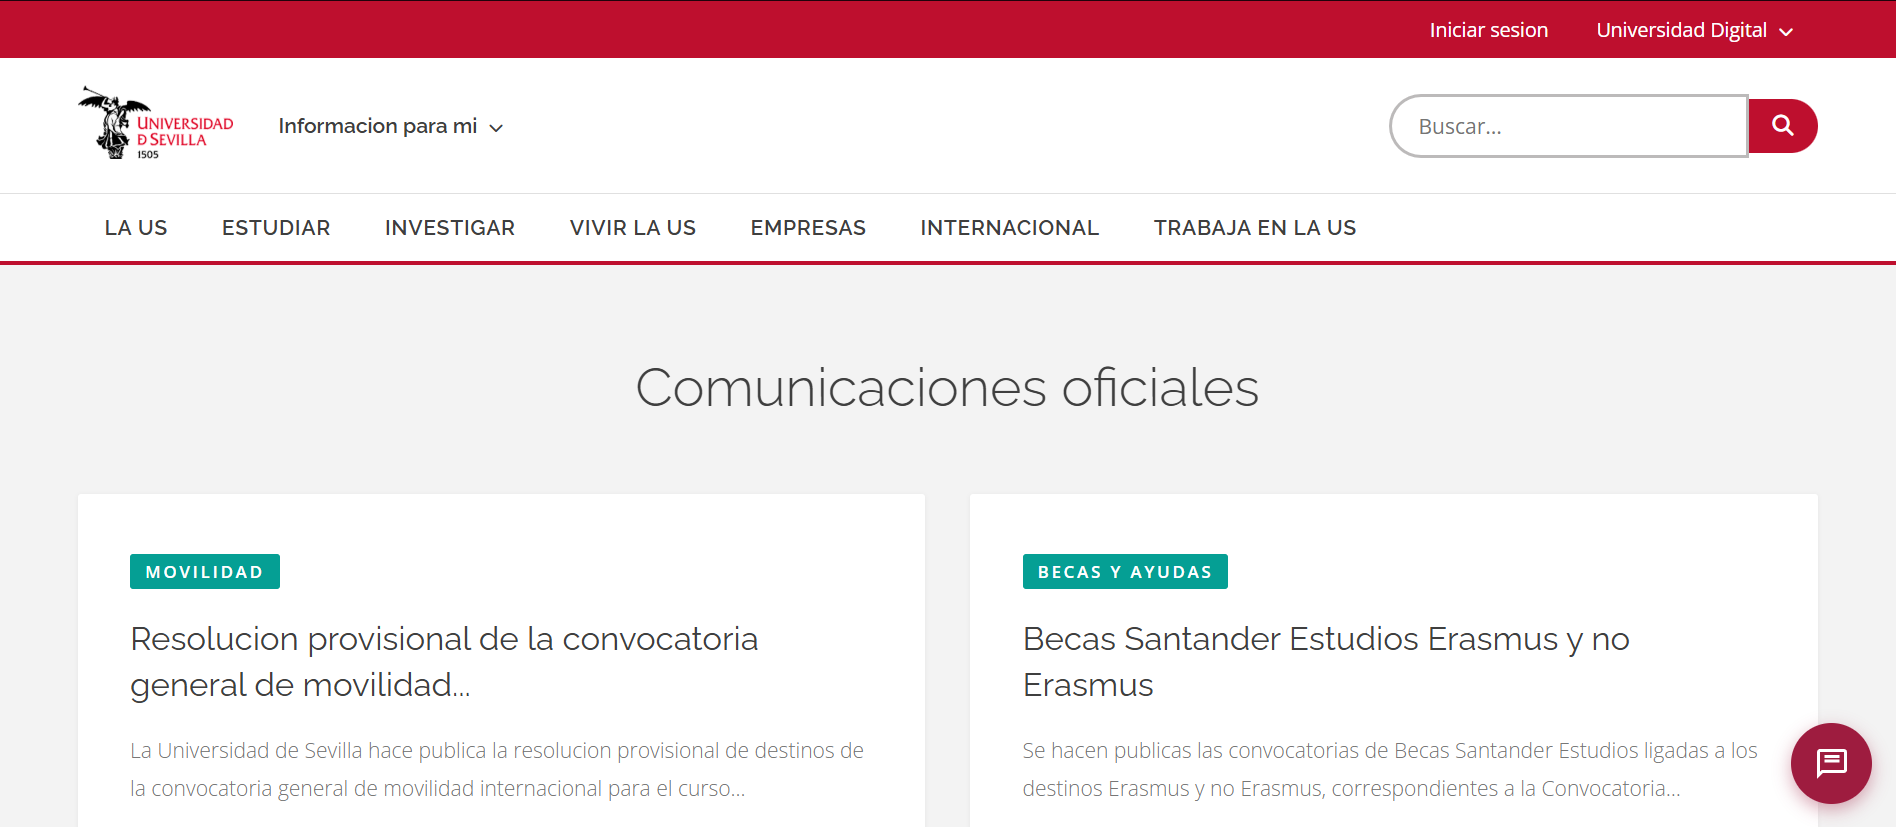
\includegraphics[width=0.95\linewidth]{img/widget_cerrado.png}
  \caption{Página principal del prototipo con el \textit{widget} de chat cerrado.}
  \label{fig:widget-cerrado}
\end{figure}

Tras desplegar el chat, el alumno encuentra un mensaje de bienvenida y, sobre él, un selector de titulación que sirve para fijar el contexto académico inicial (Figura~\ref{fig:widget-abierto}). Por defecto, la titulación seleccionada es Grado en Ingeniería Informática -- Ingeniería del Software (GII-IS), por ser la titulación con mayor cobertura informativa en el prototipo, pero el alumno puede cambiarla en cualquier momento, ya sea desde el selector o expresando el cambio en lenguaje natural durante la conversación (``cambia a tecnologías informáticas'', ``soy de IC'').

\begin{figure}[hbtp]
  \centering
  % CAPTURA: widget abierto, con el mensaje de bienvenida y el selector de
  % titulación visible. Sin conversación iniciada aún.
  % Guardar como: img/widget_abierto.png
  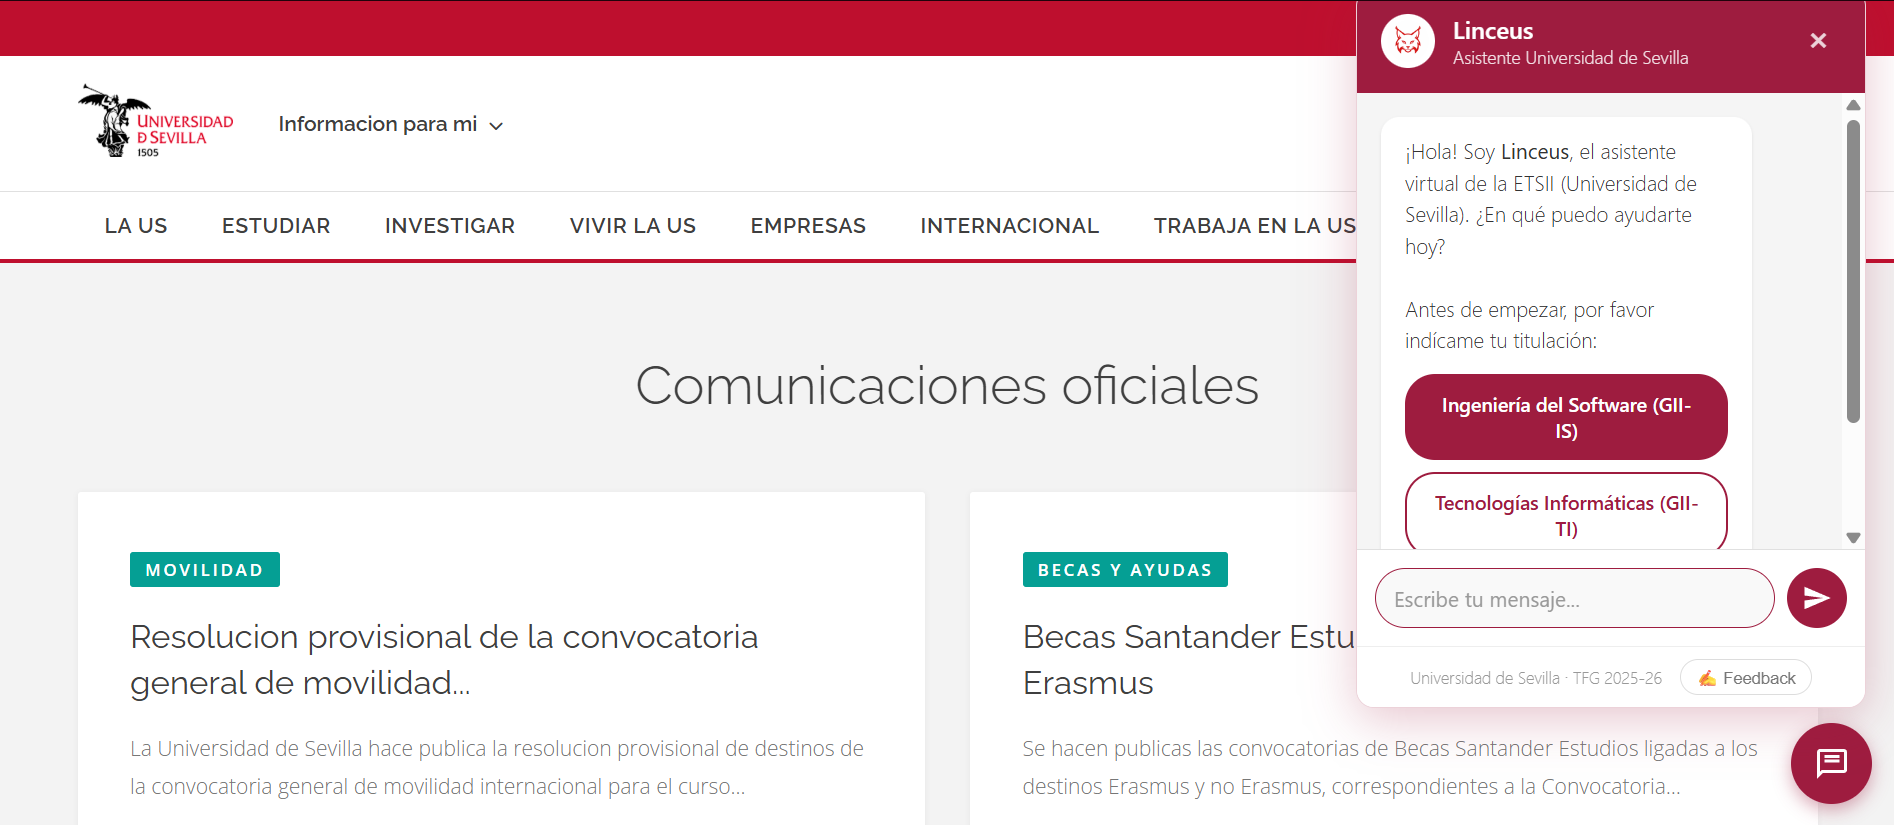
\includegraphics[width=0.95\linewidth]{img/widget_abierto.png}
  \caption{\textit{Widget} desplegado con mensaje de bienvenida y selector de titulación.}
  \label{fig:widget-abierto}
\end{figure}

\subsection{Modelo conversacional}\label{subsec:usuario-modelo}

El asistente está diseñado para responder a consultas formuladas en español natural. No es necesario emplear comandos ni una sintaxis específica: el sistema interpreta la intención del usuario a partir del texto libre y se apoya en el contexto de los turnos anteriores cuando la consulta es elíptica. Esto significa, por ejemplo, que tras preguntar por una asignatura concreta el alumno puede continuar con preguntas como ``¿y cuántos créditos tiene?'' sin necesidad de repetir el nombre.

El bot tolera errores tipográficos moderados, abreviaturas habituales (FP, ADDA, IISSI2, PSG2) y reformulaciones de la misma pregunta. Ante una consulta ambigua, el asistente solicita al usuario los datos que necesita, típicamente el curso o el grupo cuando la consulta afecta a horarios. Si la información solicitada no está disponible en la base de datos, el bot responde de forma explícita, sin inventar contenido. Las preguntas que caen fuera del ámbito académico (información meteorológica, peticiones generales no relacionadas con la universidad) se rechazan con un mensaje cortés y se redirige al usuario hacia el conjunto de funcionalidades soportadas.

\subsection{Funcionalidades disponibles}\label{subsec:usuario-funcionalidades}

El prototipo cubre tres dominios funcionales principales. La Tabla~\ref{tab:funcionalidades-usuario} resume los tipos de consulta soportados con un ejemplo representativo de cada uno.

\begin{table}[hbtp]
\centering
\caption{Tipos de consulta soportados por el prototipo.}\label{tab:funcionalidades-usuario}
\begin{tabular}{p{3.4cm}p{4cm}p{6cm}}
\hline
\textbf{Dominio} & \textbf{Tipo de consulta} & \textbf{Ejemplo de pregunta} \\
\hline
Asignaturas & Ficha individual & ``¿Qué es ADDA?'' \\
 & Listado por criterio & ``¿Qué optativas hay en cuarto?'' \\
 & Conteo & ``¿Cuántas obligatorias tiene tercero?'' \\
 & Información del plan docente & ``¿Cómo se evalúa PSG2?'' \\
\hline
Horarios & Por curso y grupo & ``Horario de segundo grupo 3'' \\
 & Por asignatura & ``¿Cuándo es ADDA?'' \\
 & Por día concreto & ``¿Qué clases hay el lunes?'' \\
 & Por aula o laboratorio & ``Laboratorio de Álgebra grupo 1'' \\
\hline
Profesorado & Datos de contacto & ``Email de Galindo'' \\
 & Profesores de una asignatura & ``¿Quiénes imparten IISSI2?'' \\
 & Coordinación & ``¿Quién coordina IA?'' \\
 & Tutorías & ``Tutorías de Bernárdez'' \\
\hline
\end{tabular}
\end{table}

Más allá de estas funcionalidades primarias, el bot incorpora dos comportamientos transversales que conviene conocer. El primero es el \textit{cambio de contexto académico}, ya mencionado, que permite consultar información de cualquiera de las tres titulaciones de la ETSII (Ingeniería del Software, Ingeniería de Computadores, Tecnologías Informáticas) cambiando dinámicamente la titulación activa. El segundo es el \textit{seguimiento conversacional}, que permite formular consultas elípticas apoyadas en los turnos anteriores: tras preguntar por una asignatura, expresiones del tipo ``¿y de qué curso es?'', ``¿y los profesores?'' o ``¿y el horario?'' resuelven correctamente la referencia implícita. La Figura~\ref{fig:conversacion-ejemplo} muestra una sesión representativa con varias de estas capacidades encadenadas.

\begin{figure}[hbtp]
  \centering
  % CAPTURA: conversación real en el widget que muestre al menos:
  %   - una consulta de asignatura (p.ej. "¿qué es ADDA?")
  %   - una pregunta de seguimiento elíptica (p.ej. "¿y cuántos créditos?")
  %   - una consulta de profesorado o cambio de titulación
  % Guardar como: img/conversacion_ejemplo.png
  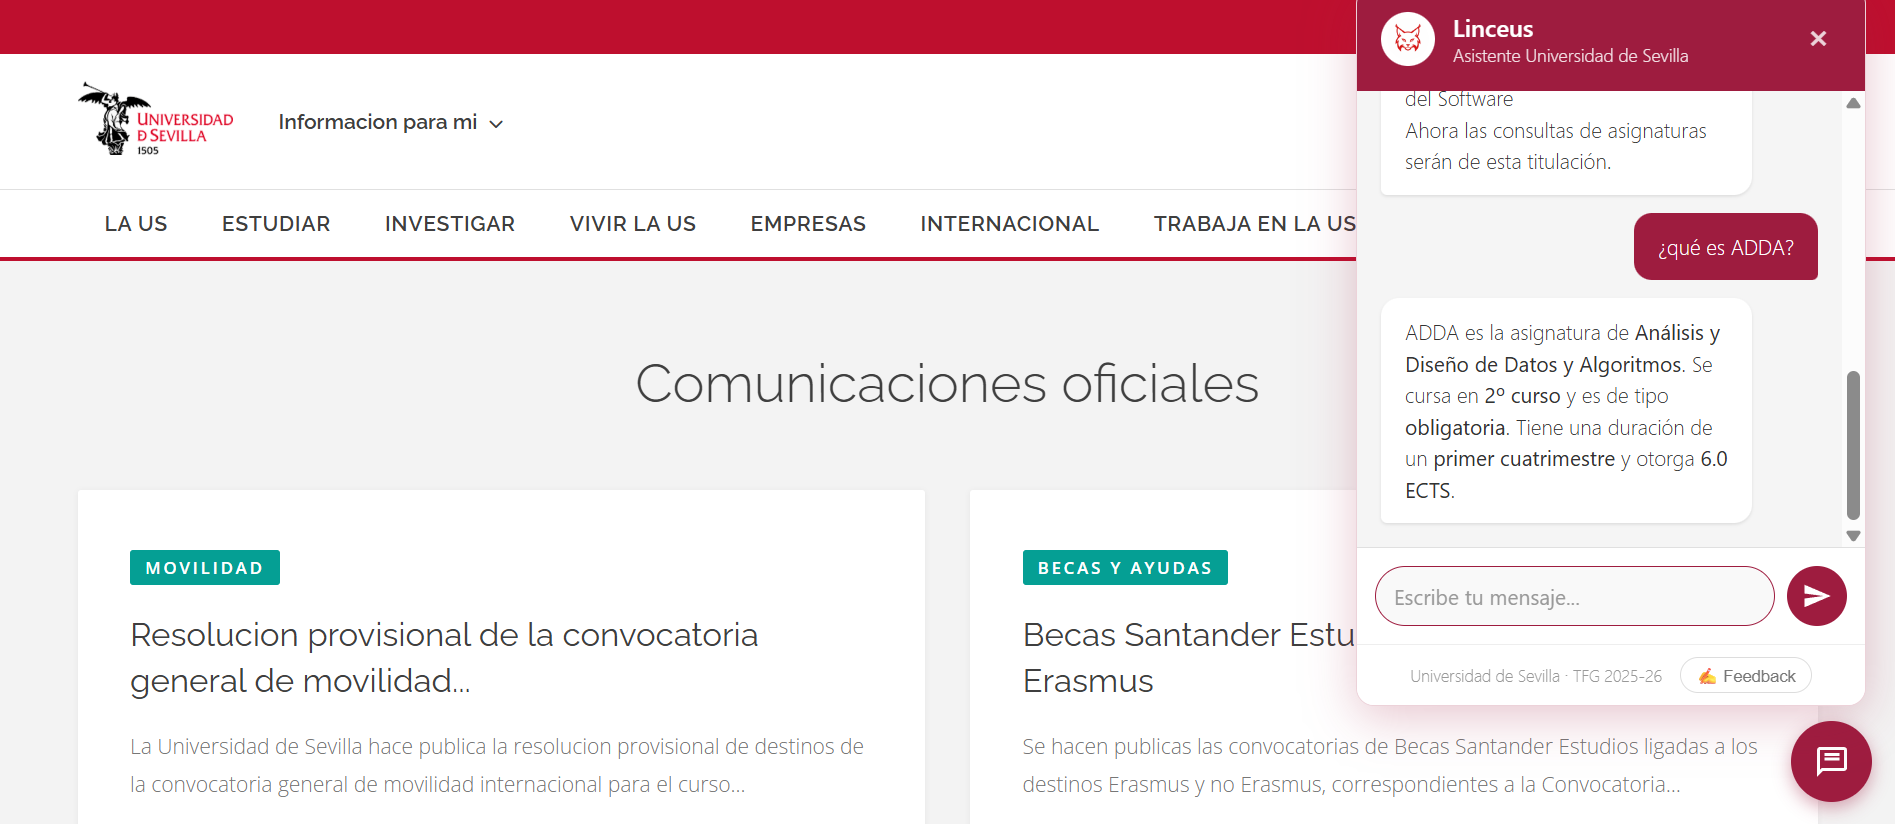
\includegraphics[width=0.95\linewidth]{img/conversacion_ejemplo.png}
  \caption{Ejemplo de sesión con seguimiento conversacional y cambio de contexto.}
  \label{fig:conversacion-ejemplo}
\end{figure}

\subsection{Recomendaciones de uso}\label{subsec:usuario-recomendaciones}

Aunque el sistema admite formulaciones libres, la calidad de la respuesta mejora cuando el alumno aporta el contexto necesario en la propia consulta. Para horarios resulta útil indicar curso y grupo desde el primer turno; para profesorado, el apellido completo o el nombre exacto reduce la ambigüedad cuando varios docentes comparten apellido. Las consultas demasiado abiertas (``cuéntame cosas de la carrera'') tienden a producir respuestas genéricas, ya que el bot no dispone de un único objetivo informativo al que dirigirse. Por último, el sistema no almacena el contenido de las conversaciones para fines comerciales y permite al usuario reportar respuestas incorrectas mediante el botón de \textit{feedback} integrado en cada turno, lo cual contribuye a la mejora continua del prototipo.

\subsection{Panel de administración}\label{subsec:usuario-admin}

El sistema incluye un panel de administración accesible en \texttt{/admin.html}, protegido por autenticación, que permite gestionar los datos académicos del prototipo sin necesidad de acceder directamente a la base de datos. El panel se organiza en cinco secciones accesibles desde la barra de navegación superior.

La vista de inicio (Figura~\ref{fig:admin-home}) muestra la jerarquía de centros y titulaciones disponibles. Desde ella se puede navegar a las asignaturas de cada titulación y consultar o actualizar su información.

\begin{figure}[hbtp]
  \centering
  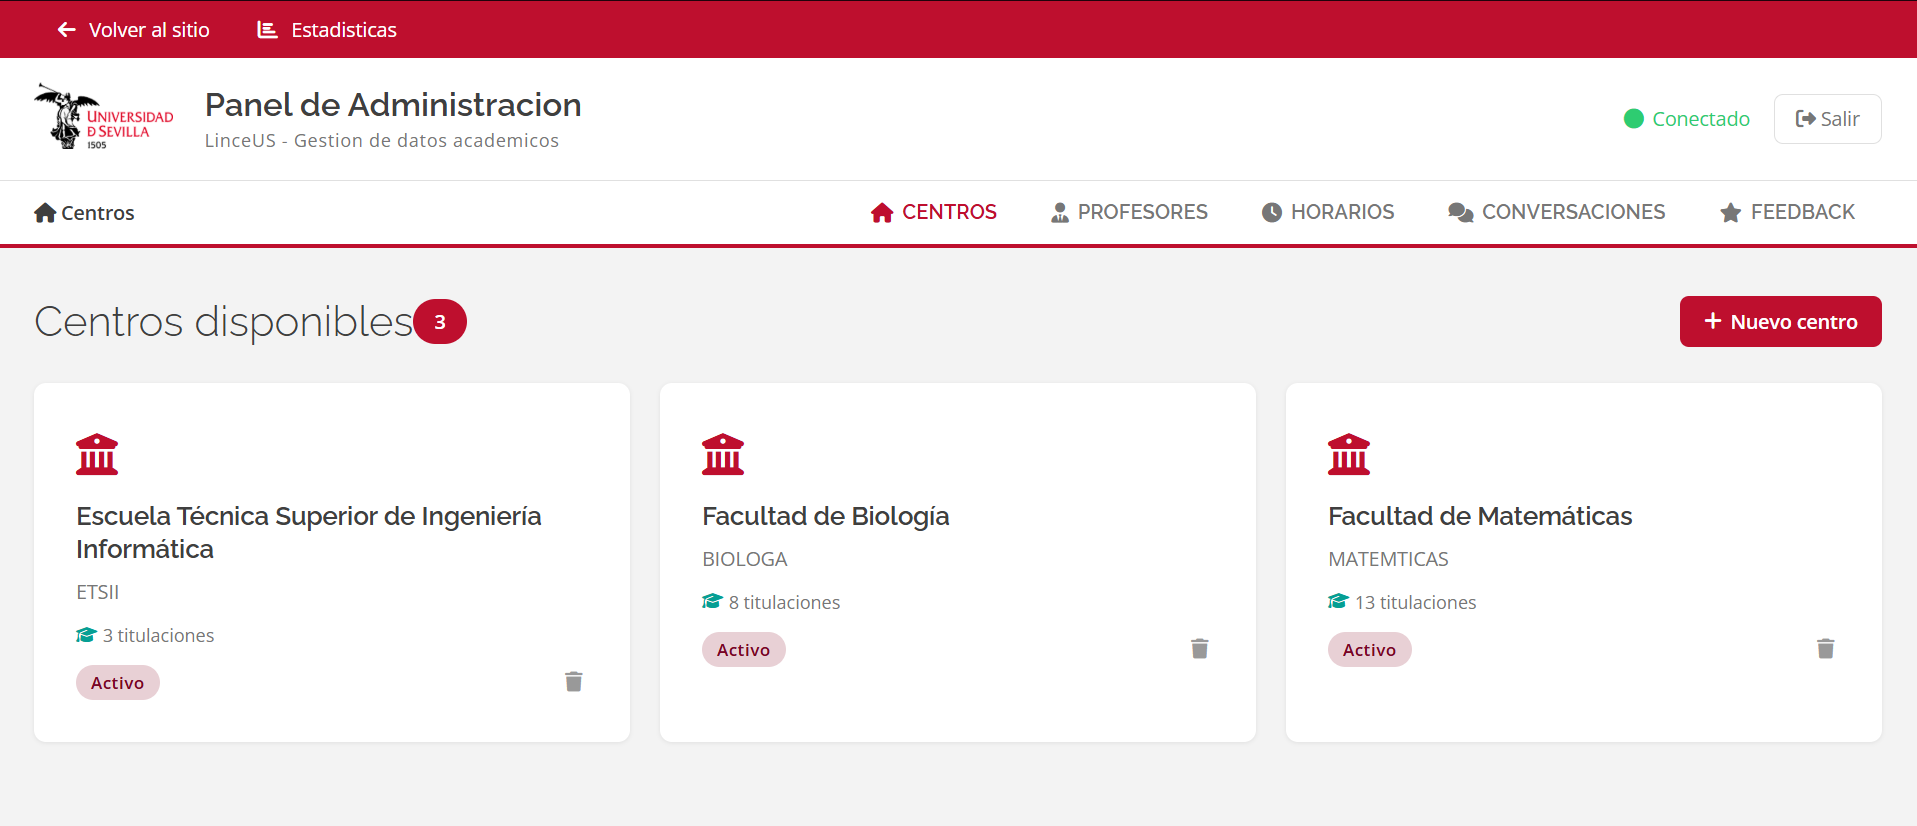
\includegraphics[width=0.95\linewidth]{img/admin_home.png}
  \caption{Panel de administración: vista de centros y titulaciones.}
  \label{fig:admin-home}
\end{figure}

La sección de profesores (Figura~\ref{fig:admin-profesores}) lista el profesorado con sus datos de contacto y permite actualizar la información directamente desde el panel, sin necesidad de re-entrenar el modelo.

\begin{figure}[hbtp]
  \centering
  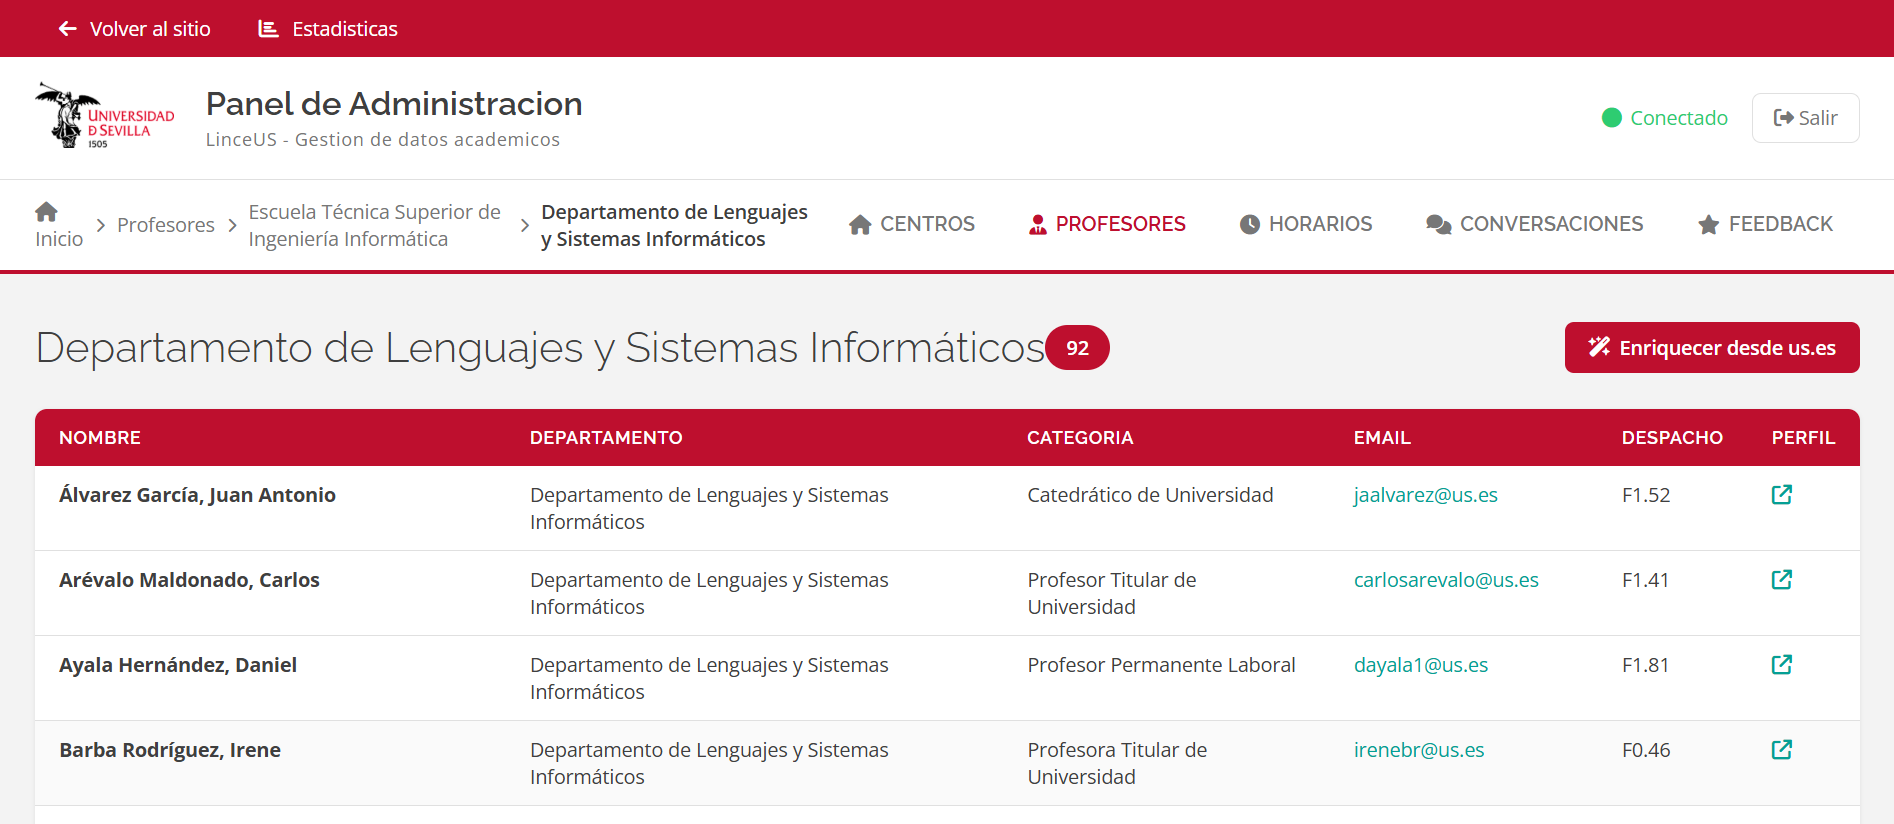
\includegraphics[width=0.95\linewidth]{img/admin_profesores.png}
  \caption{Panel de administración: gestión del profesorado.}
  \label{fig:admin-profesores}
\end{figure}

La sección de horarios (Figura~\ref{fig:man-admin-horarios}) muestra los horarios estructurados por titulación, curso y grupo, y expone los mismos datos que el chatbot consulta en tiempo real.

\begin{figure}[hbtp]
  \centering
  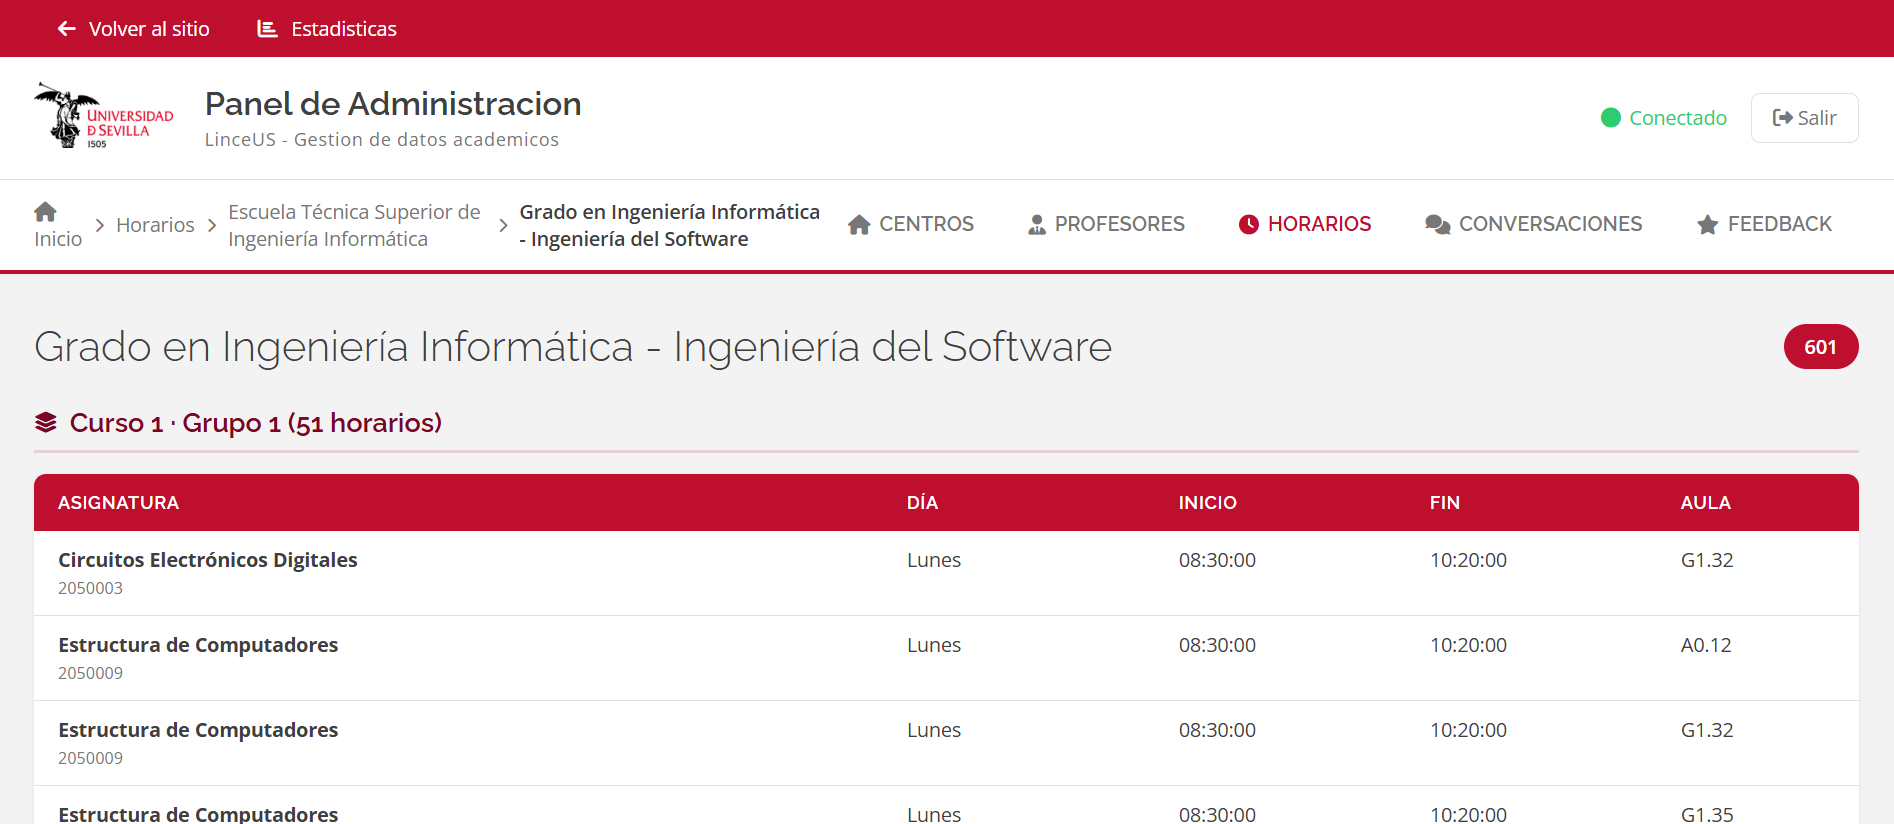
\includegraphics[width=0.95\linewidth]{img/admin_horarios.png}
  \caption{Panel de administración: vista de horarios.}
  \label{fig:man-admin-horarios}
\end{figure}

La sección de conversaciones (Figura~\ref{fig:man-admin-conversaciones}) registra las sesiones de usuario de forma anonimizada, lo que permite detectar patrones de uso, preguntas frecuentes y casos en los que el bot no proporcionó una respuesta satisfactoria.

\begin{figure}[hbtp]
  \centering
  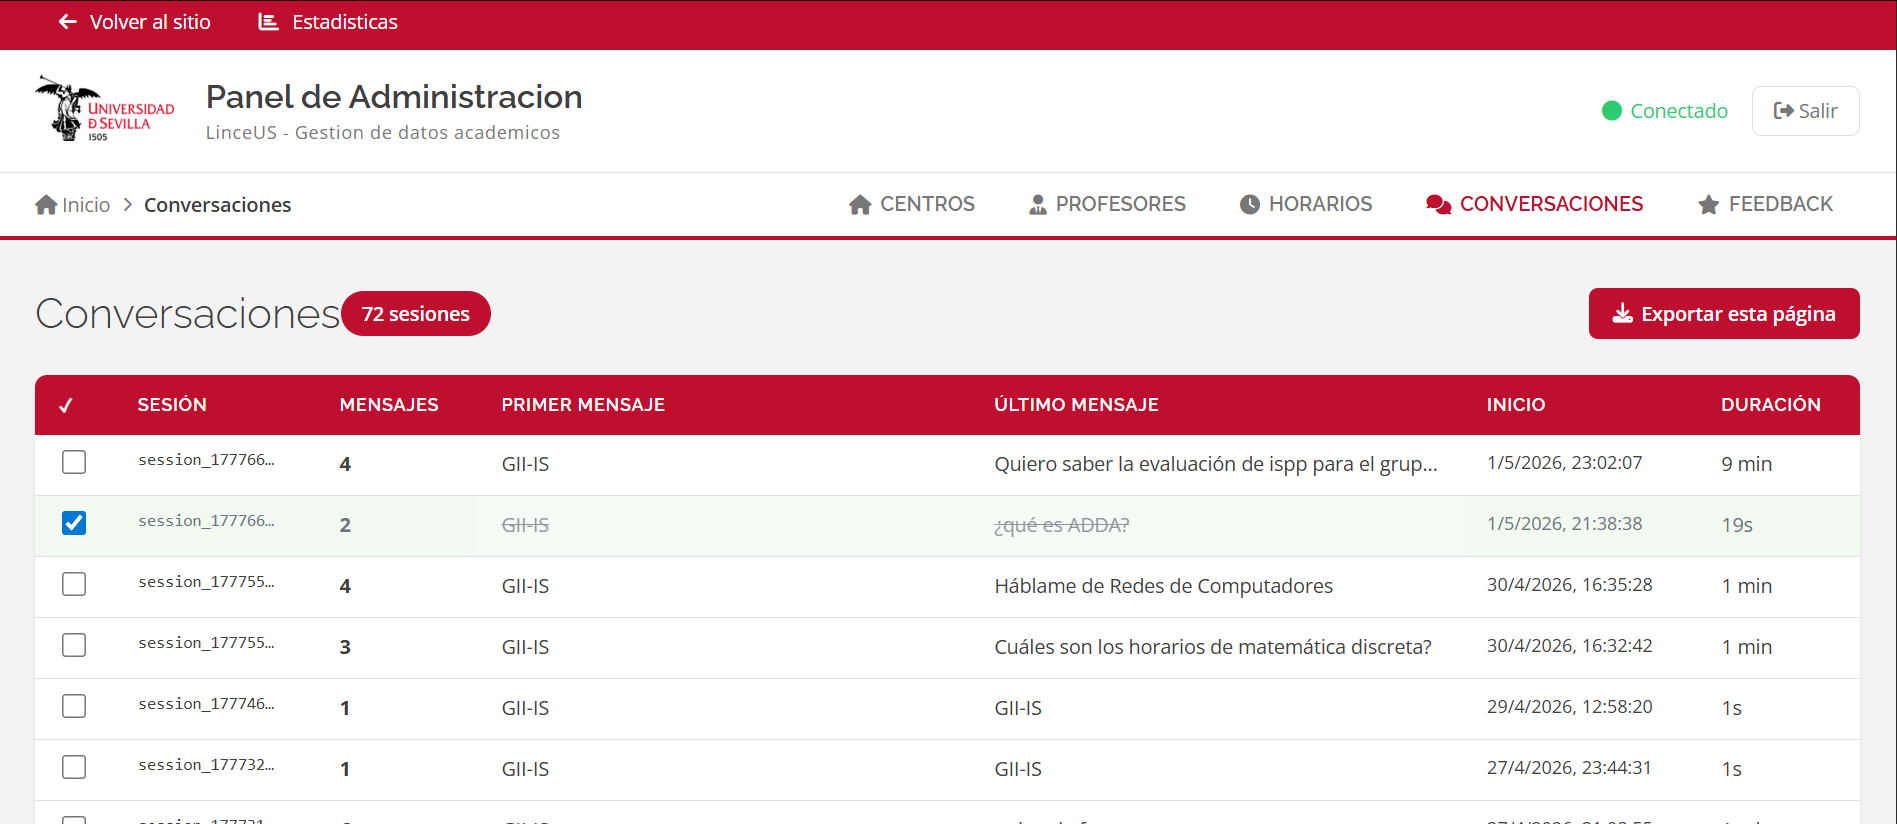
\includegraphics[width=0.95\linewidth]{img/admin_conversaciones.png}
  \caption{Panel de administración: registro de conversaciones anonimizadas.}
  \label{fig:man-admin-conversaciones}
\end{figure}

Por último, la vista de estadísticas (Figura~\ref{fig:admin-stats}) agrega métricas de uso del sistema: número de sesiones, distribución de intenciones detectadas y evolución temporal del tráfico.

\begin{figure}[hbtp]
  \centering
  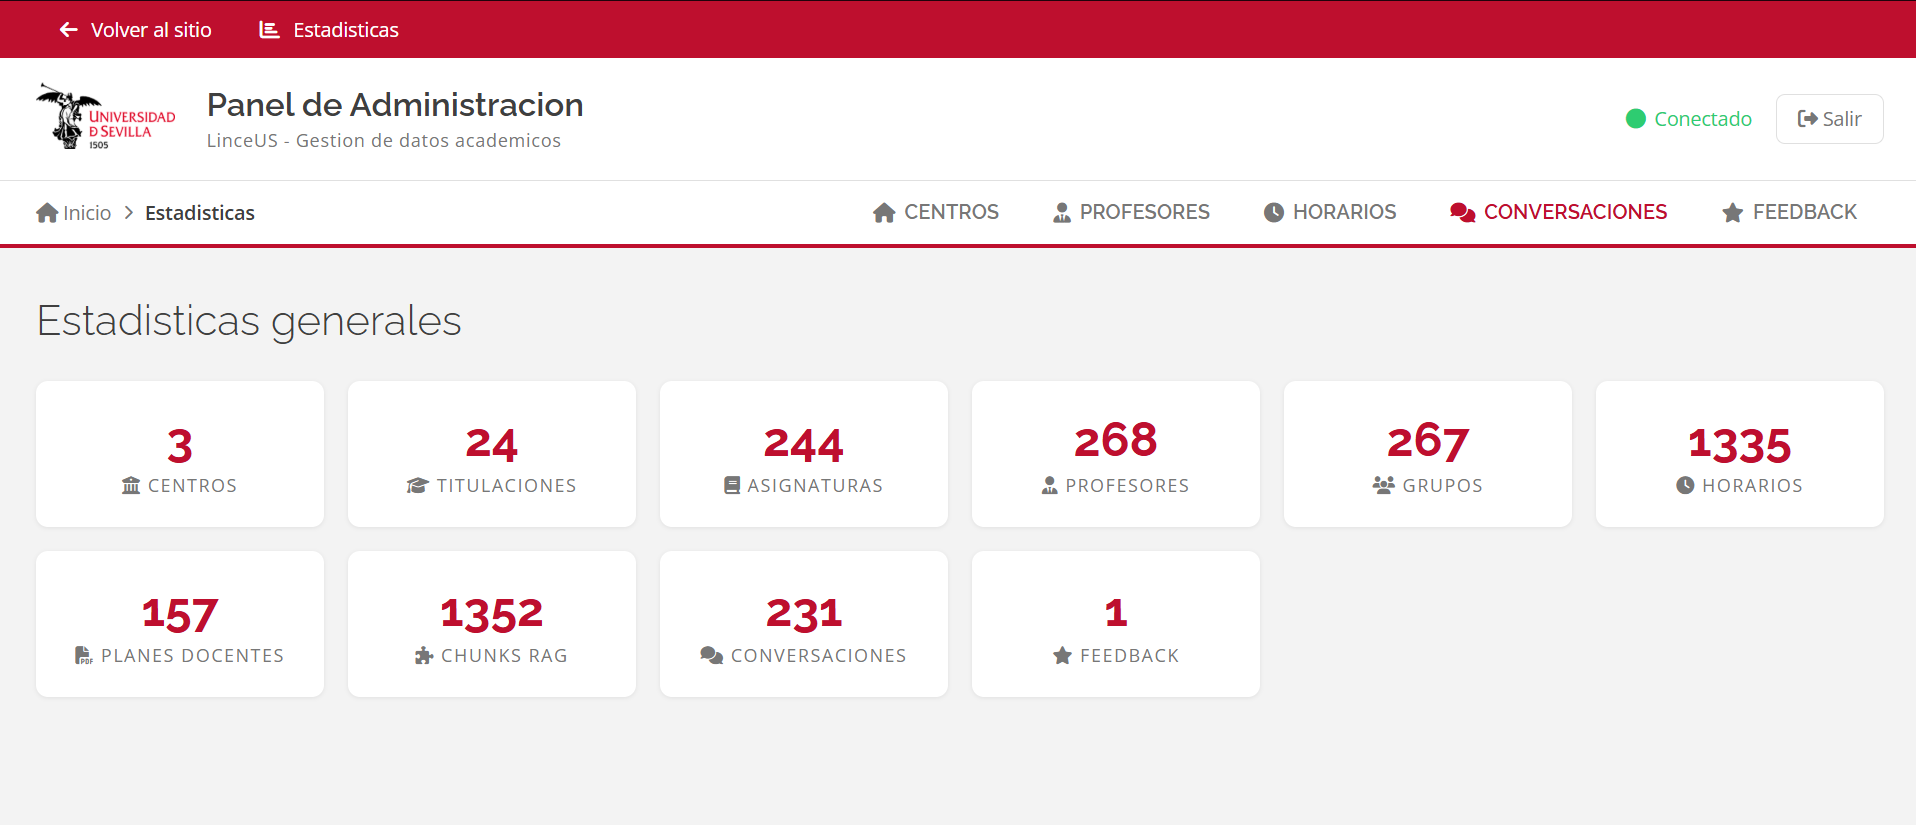
\includegraphics[width=0.95\linewidth]{img/admin_stats.png}
  \caption{Panel de administración: estadísticas de uso del sistema.}
  \label{fig:admin-stats}
\end{figure}

% =====================================================
% SECCIÓN 2: MANUAL DE DESPLIEGUE
% =====================================================
\section{Manual de despliegue}\label{sec:manual-despliegue}

El manual de despliegue describe los pasos necesarios para instalar Linceus Assistant en una infraestructura nueva, ya sea un entorno de desarrollo local o un servidor de producción. La instalación se ha diseñado para ser reproducible mediante Docker Compose, lo que evita la necesidad de instalar manualmente el conjunto de dependencias del \textit{stack} y reduce drásticamente las divergencias entre entornos.

\subsection{Requisitos previos}\label{subsec:despliegue-requisitos}

La máquina destinataria debe cumplir los requisitos mínimos recogidos en la Tabla~\ref{tab:despliegue-requisitos}. Estos requisitos se han validado sobre el \textit{droplet} de DigitalOcean utilizado durante el piloto y son suficientes para la carga prevista en la fase de prototipo (un orden de magnitud por debajo de la población total de la ETSII).

\begin{table}[hbtp]
\centering
\caption{Requisitos mínimos del entorno de despliegue.}\label{tab:despliegue-requisitos}
\begin{tabular}{ll}
\hline
\textbf{Recurso} & \textbf{Valor recomendado} \\
\hline
Sistema operativo & Linux (Ubuntu 22.04 LTS o equivalente) \\
CPU & 2 vCPU \\
Memoria RAM & 4 GB \\
Almacenamiento & 20 GB SSD \\
Docker Engine & 24.x o superior \\
Docker Compose & v2 (incluido en Docker Engine) \\
Conectividad saliente & HTTPS hacia Supabase y Google AI Studio \\
\hline
\end{tabular}
\end{table}

Además de los recursos de cómputo, el despliegue requiere disponer de tres credenciales externas: la cadena de conexión a la base de datos Supabase con extensión \texttt{pgvector}, la clave de API de Google AI Studio para el modelo Gemini y un dominio o subdominio con certificado TLS si la instalación se realiza en producción. Estas credenciales se configuran en un fichero \texttt{.env} ubicado en la raíz del proyecto, cuyo formato se describe en \texttt{.env.example}.

\subsection{Instalación}\label{subsec:despliegue-instalacion}

La instalación parte de la clonación del repositorio del proyecto y se completa en cuatro pasos. El primer paso consiste en obtener una copia local del código y situarse en el directorio resultante. El segundo paso es preparar el fichero \texttt{.env} a partir de la plantilla, sustituyendo cada variable por el valor correspondiente al entorno de despliegue. El tercer paso es asegurarse de que el directorio \texttt{models/} contiene un modelo Rasa entrenado: si no es así, basta con ejecutar \texttt{rasa train} en un entorno con las dependencias instaladas, o bien copiar el último modelo válido desde el repositorio. El cuarto y último paso es levantar la pila completa con Docker Compose:

\begin{lstlisting}[language=bash, caption={Levantar la pila completa con Docker Compose.}]
git clone <url-repositorio> && cd linceus-assistant
cp .env.example .env          # completar variables
docker compose -f docker/docker-compose.yml up --build -d
\end{lstlisting}

La opción \texttt{-d} ejecuta los contenedores en segundo plano. El primer arranque construye las imágenes correspondientes, lo que puede tardar varios minutos en función del ancho de banda disponible para descargar las dependencias. A partir de ese momento, los rearranques posteriores son cuestión de pocos segundos, salvo que se hayan modificado las dependencias de Python.

\subsection{Arquitectura del despliegue}\label{subsec:despliegue-arquitectura}

La pila se compone de cuatro contenedores que se comunican entre sí a través de la red interna de Docker, recogidos en la Tabla~\ref{tab:despliegue-contenedores}. Únicamente el contenedor de \textit{frontend} expone el puerto 80 al exterior; el resto de servicios son accesibles solo desde el interior de la red, salvo que el operador decida exponerlos explícitamente para fines de depuración.

\begin{table}[hbtp]
\centering
\caption{Contenedores del despliegue y responsabilidad de cada uno.}\label{tab:despliegue-contenedores}
\begin{tabular}{llll}
\hline
\textbf{Contenedor} & \textbf{Imagen base} & \textbf{Versión} & \textbf{Responsabilidad} \\
\hline
\texttt{frontend} & \texttt{nginx:alpine} & alpine & Sirve los ficheros estáticos y actúa como \textit{proxy} \\
\texttt{rasa} & \texttt{rasa/rasa} & 3.6.21 + spaCy & Gestor del diálogo y NLU (puerto 5005) \\
\texttt{actions} & \texttt{python:3.10.14-slim-bookworm} & 3.10.14 & Acciones personalizadas y módulo RAG \\
\texttt{admin} & \texttt{python:3.10-slim} & 3.10 & API Flask del panel de administración \\
\hline
\end{tabular}
\end{table}

El contenedor de \textit{actions} monta los directorios \texttt{actions/} y \texttt{rag/} como volúmenes, lo que permite recargar los cambios en caliente sin reconstruir la imagen. El contenedor de Rasa monta los ficheros de configuración (\texttt{config.yml}, \texttt{domain.yml}, \texttt{credentials.yml}) y un fichero específico de \textit{endpoints} que enruta el servidor hacia el contenedor de \textit{actions} a través del nombre de servicio interno. El contenedor de \textit{frontend} inyecta la variable \texttt{RASA\_SERVER} en los ficheros estáticos en el momento del arranque mediante un \textit{script} de \textit{entrypoint}, lo que evita tener que recompilar el \textit{frontend} para distintos entornos.

\subsection{Verificación del despliegue}\label{subsec:despliegue-verificacion}

Una vez levantada la pila, la verificación del despliegue se realiza siguiendo cuatro comprobaciones en orden. En primer lugar, la página principal debe estar accesible en \texttt{http://<host>/}, donde \texttt{<host>} es la dirección o dominio del servidor. En segundo lugar, el panel de administración debe estar accesible en \texttt{http://<host>/admin.html} y permitir consultar la lista de centros y titulaciones. En tercer lugar, el \textit{widget} de chat debe responder a un mensaje de prueba simple (``hola'') con un saludo personalizado, lo cual confirma que el camino completo entre \textit{frontend}, Rasa, \textit{actions} y modelo Gemini está operativo. Por último, una consulta sencilla con dependencia de base de datos (``¿cuántas asignaturas tiene primero?'') debe devolver una cifra coherente con los datos cargados, lo cual confirma la conectividad con Supabase.

Si alguna de estas comprobaciones falla, los registros de cada contenedor se consultan con la orden recogida en el Código~\ref{lst:logs}, donde \texttt{<servicio>} es uno de los cuatro nombres recogidos en la Tabla~\ref{tab:despliegue-contenedores}. El error más habitual durante la primera puesta en marcha es la falta de un modelo entrenado en \texttt{models/}, lo que provoca que el contenedor de Rasa se reinicie en bucle.

\begin{lstlisting}[language=bash, caption={Consultar registros de un contenedor.}, label={lst:logs}]
docker compose -f docker/docker-compose.yml logs -f <servicio>
# Ejemplo: ver logs del servidor Rasa en tiempo real
docker compose -f docker/docker-compose.yml logs -f rasa
\end{lstlisting}

\subsection{Operaciones habituales}\label{subsec:despliegue-operaciones}

El día a día del operador se concentra en un puñado de tareas rutinarias. Los cambios en el código de \textit{actions} o del módulo RAG no requieren reiniciar nada, ya que el \textit{action server} se ejecuta con la opción \texttt{--auto-reload}. Los cambios en el modelo Rasa (re-entrenamiento) requieren detener y volver a arrancar el contenedor \texttt{rasa} para que recargue el modelo desde el volumen \texttt{models/}. Las actualizaciones de las dependencias de Python requieren reconstruir la imagen afectada antes de volver a levantarla. Las copias de seguridad de la base de datos se gestionan desde el panel de Supabase, que dispone de \textit{snapshots} automáticos diarios; el código del proyecto no almacena estado mutable en disco fuera de la base de datos.

\begin{lstlisting}[language=bash, caption={Operaciones de mantenimiento habituales.}]
# Recargar modelo Rasa tras reentrenamiento
docker compose -f docker/docker-compose.yml restart rasa

# Reconstruir imagen tras cambio de dependencias Python
docker compose -f docker/docker-compose.yml build actions
docker compose -f docker/docker-compose.yml up -d actions

# Detener toda la pila
docker compose -f docker/docker-compose.yml down
\end{lstlisting}

% =====================================================
% SECCIÓN 3: MANUAL DE DESARROLLO
% =====================================================
\section{Manual de desarrollo}\label{sec:manual-desarrollo}

El manual de desarrollo se dirige a quien deba modificar, ampliar o mantener el código de Linceus Assistant tras el cierre de este TFG. Su objetivo es minimizar la curva de aprendizaje proporcionando una visión panorámica del repositorio, las convenciones empleadas y el ciclo de trabajo recomendado.

\subsection{Estructura del repositorio}\label{subsec:desarrollo-estructura}

El repositorio sigue la disposición habitual de un proyecto Rasa con extensiones específicas para el módulo RAG y el panel de administración. La Tabla~\ref{tab:desarrollo-estructura} recoge los directorios de primer nivel y su responsabilidad.

\begin{table}[hbtp]
\centering
\caption{Estructura del repositorio Linceus Assistant.}\label{tab:desarrollo-estructura}
\begin{tabular}{ll}
\hline
\textbf{Directorio} & \textbf{Contenido} \\
\hline
\texttt{actions/} & Acciones personalizadas (Python) que ejecuta el \textit{action server} \\
\texttt{admin/} & Aplicación Flask del panel de administración \\
\texttt{data/} & Conjuntos de datos NLU y \textit{stories} para Rasa \\
\texttt{docker/} & Ficheros de Compose y \textit{Dockerfile} de cada servicio \\
\texttt{frontend/} & \textit{Widget} de chat y panel HTML/CSS/JS \\
\texttt{models/} & Modelos Rasa entrenados (no versionados) \\
\texttt{rag/} & Módulo de recuperación aumentada por generación \\
\texttt{tests/} & Suite de aceptación funcional y planes de prueba \\
\hline
\end{tabular}
\end{table}

Los ficheros de configuración principales (\texttt{config.yml}, \texttt{domain.yml}, \texttt{credentials.yml}, \texttt{endpoints.yml} y \texttt{endpoints.docker.yml}) residen en la raíz, junto con los ficheros de dependencias \texttt{requirements-rasa.txt} y \texttt{requirements-actions.txt}. La documentación específica de cada componente se encuentra en su propio fichero \texttt{README.md}, mientras que el \texttt{README.md} de la raíz centraliza las instrucciones de arranque local y con Docker.

\subsection{Entorno de desarrollo}\label{subsec:desarrollo-entorno}

El entorno de desarrollo recomendado se basa en Python 3.10 dentro de un entorno virtual. Tras clonar el repositorio, los pasos habituales son los del Código~\ref{lst:dev-setup}.

\begin{lstlisting}[language=bash, caption={Preparacion del entorno de desarrollo local.}, label={lst:dev-setup}]
python3.10 -m venv .venv && source .venv/bin/activate
pip install -r requirements-rasa.txt -r requirements-actions.txt
cp .env.example .env          # completar con claves reales
rasa train                    # genera models/linceus_vX.Y.Z.tar.gz
\end{lstlisting}

A partir de ese momento, los cuatro componentes (Rasa, \textit{action server}, panel y \textit{frontend}) pueden levantarse en terminales independientes según se documenta en el \texttt{README.md} principal. Los comandos del Código~\ref{lst:dev-run} arrancan el flujo completo sin Docker.

\begin{lstlisting}[language=bash, caption={Arranque de los componentes en modo desarrollo.}, label={lst:dev-run}]
# Terminal 1: servidor Rasa
rasa run --enable-api --cors "*" --port 5005 --endpoints endpoints.yml

# Terminal 2: action server (recarga automatica al guardar)
rasa run actions --port 5055 --auto-reload

# Terminal 3: panel de administracion Flask
python -m admin.app

# Terminal 4: frontend (servir estaticos)
cd frontend && python -m http.server 8080
\end{lstlisting}

Durante el desarrollo, la opción \texttt{--auto-reload} del \textit{action server} y la naturaleza estática del \textit{frontend} permiten iterar rápidamente sobre la mayoría de los cambios. Los cambios en el modelo NLU o en el dominio de Rasa requieren un nuevo entrenamiento, que en una máquina convencional toma alrededor de uno o dos minutos. Los cambios en la estructura de la base de datos se gestionan a través del editor de tablas de Supabase y deben propagarse manualmente al fichero \texttt{schema.sql} de referencia.

\subsection{Ciclo de incorporación de cambios}\label{subsec:desarrollo-ciclo}

El proyecto sigue un flujo de trabajo basado en \textit{feature branches} sobre la rama principal \texttt{main}. Cada cambio se desarrolla en una rama propia, se valida localmente mediante la suite de pruebas pertinente y se integra a través de una solicitud de incorporación que se revisa antes de fusionar. El ciclo se compone de cinco etapas, descritas en la Tabla~\ref{tab:desarrollo-ciclo}.

\begin{table}[hbtp]
\centering
\caption{Etapas del ciclo de incorporación de cambios.}\label{tab:desarrollo-ciclo}
\begin{tabular}{p{3.5cm}p{9cm}}
\hline
\textbf{Etapa} & \textbf{Descripción} \\
\hline
1. Diseño & Definición del cambio en términos de requisito o defecto. Si el cambio afecta al NLU, se preparan ejemplos adicionales para \texttt{nlu.yml}. \\
2. Implementación & Modificación del código en la rama de trabajo, siguiendo las convenciones de estilo de Python (PEP 8) y de Rasa. \\
3. Pruebas locales & Ejecución de \texttt{rasa test core} para la política, \texttt{run\_test\_plan.py} para la suite E2E pertinente y revisión manual de los casos afectados. \\
4. Integración & Solicitud de incorporación a \texttt{main} con descripción de los cambios y de los casos de prueba afectados. \\
5. Despliegue & Reconstrucción de los contenedores afectados y verificación en el entorno de pruebas antes de promocionar a producción. \\
\hline
\end{tabular}
\end{table}

\subsection{Cómo añadir una nueva intención}\label{subsec:desarrollo-intencion}

La incorporación de una nueva intención conversacional es la operación más frecuente durante la evolución del bot, y el procedimiento es suficientemente representativo como para servir de ilustración del ciclo completo.

El primer paso es declarar la intención en \texttt{domain.yml} y añadir entre quince y veinte ejemplos representativos en \texttt{data/nlu.yml}, procurando cubrir tanto formulaciones limpias como con errores tipográficos habituales. El Código~\ref{lst:nlu-intent} muestra la estructura de un bloque de ejemplos típico:

\begin{lstlisting}[language=python, caption={Declaracion de una intencion con ejemplos NLU en \texttt{data/nlu.yml}.}, label={lst:nlu-intent}]
- intent: consulta_creditos_asignatura
  examples: |
    - cuantos creditos tiene [ADDA](nombre_asignatura)
    - cuantos creditos son de [Redes](nombre_asignatura)
    - creditos de [PSG2](nombre_asignatura)
    - de cuantos creditos es [IISSI2](nombre_asignatura)
    - [FP](nombre_asignatura) cuantos creditos
\end{lstlisting}

El segundo paso es definir, si procede, los \textit{slots} y entidades que la intención necesita extraer; estos también se declaran en \texttt{domain.yml} y se entrenan automáticamente con el modelo. El tercer paso es escribir la acción personalizada en \texttt{actions/} si la intención requiere consultar la base de datos o el módulo RAG, registrándola tanto en el dominio como en \texttt{actions/\_\_init\_\_.py}. El Código~\ref{lst:action-estructura} muestra la estructura mínima de una acción:

\begin{lstlisting}[language=python, caption={Estructura minima de una accion personalizada en Rasa.}, label={lst:action-estructura}]
from rasa_sdk import Action, Tracker
from rasa_sdk.executor import CollectingDispatcher
from rasa_sdk.events import SlotSet

class ActionConsultaCreditos(Action):

    def name(self) -> str:
        return "action_consulta_creditos"

    def run(self, dispatcher: CollectingDispatcher,
            tracker: Tracker,
            domain: dict) -> list:
        nombre = tracker.get_slot("nombre_asignatura")
        # ... consultar BD y generar respuesta
        dispatcher.utter_message(text=f"{nombre} tiene 6 creditos ECTS.")
        return [SlotSet("ultimo_nombre_asignatura", nombre)]
\end{lstlisting}

El cuarto paso es añadir las \textit{stories} correspondientes en \texttt{data/stories.yml} para que la política aprenda a enrutar correctamente la nueva intención. El quinto paso es entrenar el modelo, validar la intención con casos manuales y, si la cobertura es razonable, añadir uno o dos casos de aceptación a \texttt{tests/run\_test\_plan.py} para garantizar que la nueva funcionalidad no se regresa en futuros cambios.

\subsection{Buenas prácticas y convenciones}\label{subsec:desarrollo-convenciones}

A lo largo del desarrollo se han adoptado un conjunto de convenciones que conviene mantener en futuras iteraciones. Las acciones personalizadas se nombran con el prefijo \texttt{action\_} seguido del verbo principal del flujo (\texttt{action\_consulta\_profesor}, \texttt{action\_cambiar\_contexto}). Los \textit{slots} cuya función es persistir la última entidad consultada llevan el prefijo \texttt{ultimo\_} (\texttt{ultimo\_nombre\_asignatura}, \texttt{ultimo\_profesor\_consultado}). Los identificadores de los casos de prueba siguen un patrón de letra mayúscula seguido de tipo y número, donde la letra inicial alude a la categoría (\texttt{E} para asignaturas específicas, \texttt{H} para horarios, \texttt{P} para profesores, \texttt{C} para conteo, \texttt{L} para listado, \texttt{X} para cross-dominio, \texttt{F} y \texttt{R} para casos fuera de ámbito y \textit{jailbreak}). Cada decisión de diseño no trivial se documenta como una entrada \texttt{D-XXX} en el fichero correspondiente del repositorio, lo que facilita reconstruir el porqué de un comportamiento al cabo del tiempo.

El Código~\ref{lst:validar-sql} ilustra un patrón de diseño transversal al proyecto: la separación entre generación y validación. El módulo \texttt{text\_to\_sql} delega en Gemini la generación de SQL en lenguaje natural, pero antes de ejecutar cualquier \textit{query} la pasa por una función de validación que rechaza instrucciones de escritura, tablas no autorizadas y columnas fuera del esquema permitido. Este patrón evita que un fallo en el LLM pueda comprometer la integridad de la base de datos.

\begin{lstlisting}[language=python, caption={Fragmento de \texttt{validar\_sql}: lista de palabras prohibidas y verificacion de tabla.}, label={lst:validar-sql}]
# actions/asignaturas/text_to_sql.py
PALABRAS_PROHIBIDAS = [
    'INSERT', 'UPDATE', 'DELETE', 'DROP', 'ALTER', 'CREATE',
    'TRUNCATE', 'EXEC', 'UNION SELECT', 'OR 1=1', 'SLEEP(',
]
TABLAS_PERMITIDAS = {'ASIGNATURAS', 'TITULACIONES'}

def validar_sql(sql: str, tipo: str = 'select') -> Optional[str]:
    sql_upper = sql.upper().strip()
    for palabra in PALABRAS_PROHIBIDAS:
        if palabra in sql_upper:
            return None          # rechazar silenciosamente
    if not sql_upper.startswith('SELECT'):
        return None
    tablas = re.findall(r'FROM\s+(\w+)|JOIN\s+(\w+)', sql_upper)
    tablas_flat = {t for grupo in tablas for t in grupo if t}
    if tablas_flat - TABLAS_PERMITIDAS:
        return None
    return sql
\end{lstlisting}

Por último, conviene recordar que toda modificación que afecte al comportamiento del bot debe acompañarse de la actualización de los ejemplos NLU correspondientes y de un nuevo caso de aceptación. La experiencia acumulada durante el TFG demuestra que las regresiones más costosas de detectar son las que se producen en flujos colaterales tras un cambio aparentemente local; mantener la suite de aceptación actualizada es la principal salvaguarda frente a este tipo de error.

     % !TEX root = ../proyect.tex

\chapter{Conclusiones y desarrollos futuros}\label{cap:conclusiones}

Este capítulo cierra la memoria del trabajo. Tras un proyecto extenso conviene levantar la vista del detalle técnico y revisar qué se planteó al inicio, qué ha quedado efectivamente construido y qué queda por hacer. La estructura del capítulo reproduce ese orden: se sintetiza el estado final del sistema con un cuadro de indicadores, se contrastan los objetivos enunciados en el Capítulo~\ref{cap:introduccion} con la evidencia recogida durante la validación, se recopilan las lecciones aprendidas a lo largo del desarrollo, se analiza la desviación de la planificación inicial, se enumeran las líneas de evolución previstas para una segunda iteración del sistema, se discuten las consideraciones éticas y se cierra con una reflexión personal sobre la experiencia.

\section{Linceus en números}\label{sec:linceus-numeros}

Antes de revisar el cumplimiento de objetivos conviene fijar el tamaño y la cobertura efectiva del sistema en el momento del cierre. La Tabla~\ref{tab:linceus-numeros} agrupa los indicadores principales en cuatro bloques (alcance funcional, validación, métricas no funcionales y proceso de desarrollo). Todas las cifras son trazables al artefacto de origen citado en la columna derecha.

\begin{table}[hbtp]
\centering
\small
\caption{Indicadores cuantitativos de Linceus Assistant al cierre del prototipo (26/04/2026).}\label{tab:linceus-numeros}
\begin{tabular}{|p{5.4cm}|p{2.0cm}|p{4.6cm}|}
\hline
\textbf{Indicador} & \textbf{Valor} & \textbf{Fuente} \\ \hline
\multicolumn{3}{|l|}{\textit{Alcance funcional}} \\ \hline
Intenciones NLU definidas (activas) & 36 (34) & \texttt{domain.yml} \\ \hline
Entidades NLU & 10 & \texttt{domain.yml} \\ \hline
\textit{Stories} de entrenamiento & 37 & \texttt{data/stories.yml} \\ \hline
Reglas activas & 20 & \texttt{data/rules.yml} \\ \hline
\textit{Custom actions} activas & 14 & \texttt{actions/} \\ \hline
Archivos NLU por dominio & 5 & \texttt{data/nlu/} \\ \hline
Titulaciones soportadas & 3 (GII-IS, IC, TI) & Sección~\ref{sec:req-actores} \\ \hline
\multicolumn{3}{|l|}{\textit{Validación funcional}} \\ \hline
Casos E2E (PASS / total) & 150 / 159 (94,3~\%) & Tabla~\ref{tab:e2e-categorias} \\ \hline
RAG \textit{baseline} (PASS / total) & 47 / 50 (94,0~\%) & Sección~\ref{subsec:rag-baseline} \\ \hline
RAG profundidad (OK / total) & 68 / 74 (91,9~\%) & Tabla~\ref{tab:rag-cobertura} \\ \hline
NLU + Policy (acciones correctas) & 158 / 158 (100~\%) & Tabla~\ref{tab:nlu-resultados} \\ \hline
Tráfico real piloto (sesiones PASS) & 58 / 59 (98,3~\%) & Tabla~\ref{tab:trafico-resultados} \\ \hline
Suite admin \textit{pytest} (PASS / total) & 24 / 24 (100~\%) & Tabla~\ref{tab:admin-resultados} \\ \hline
Turnos auditados en piloto & 201 / 203 & Sección~\ref{subsec:trafico-resultados} \\ \hline
\multicolumn{3}{|l|}{\textit{Métricas no funcionales}} \\ \hline
Latencia mediana (p50) & 3,4 s & Tabla~\ref{tab:latencia} \\ \hline
Latencia p95 & 10,5 s & Tabla~\ref{tab:latencia} \\ \hline
Coste medio por turno (Gemini) & 0,012 cts & Sección~\ref{subsec:no-funcional-coste} \\ \hline
Llamadas a Gemini medidas & 216 & Sección~\ref{sec:pruebas-no-funcional} \\ \hline
Tiempo de cumplimiento RNF-14 (primera consulta) & 28 s (mediana) & Tabla~\ref{tab:rnf} \\ \hline
\multicolumn{3}{|l|}{\textit{Proceso de desarrollo}} \\ \hline
\textit{Sprints} completados & 8 & Capítulo~\ref{cap:planificacion} \\ \hline
Decisiones técnicas documentadas & 72 (D-001 a D-072) & \texttt{docs/sprints/} \\ \hline
Esfuerzo estimado total & $\sim$300 h & Sección~\ref{sec:conc-desviacion} \\ \hline
\end{tabular}
\end{table}

Los porcentajes superan en todas las capas su umbral académico de referencia con un margen razonable y los indicadores de proceso (72 decisiones documentadas, 8 \textit{sprints} cerrados con incremento desplegable) avalan que la cifra de validación es producto de un desarrollo trazable y no de un ajuste \textit{ad hoc} en la fase final.

\section{Cumplimiento de objetivos}\label{sec:conc-objetivos}

El Capítulo~\ref{cap:introduccion} planteaba un objetivo general y un conjunto de objetivos técnicos y académicos. Resulta razonable revisar uno por uno hasta qué punto se han alcanzado, apoyándose en la evidencia recopilada en el Capítulo~\ref{cap:pruebas}.

\subsection{Objetivo general}\label{subsec:conc-obj-general}

El objetivo general consistía en diseñar y desarrollar un asistente conversacional que ofreciera al alumnado de la Universidad de Sevilla un punto de acceso centralizado, accesible y eficiente a la información académica y administrativa. Tras el cierre del prototipo, este objetivo puede considerarse alcanzado en su versión correspondiente a la fase 1: el sistema cubre las tres épicas funcionales previstas (asignaturas, profesorado y horarios), responde correctamente al 94,3\,\% de los casos de la suite de aceptación funcional y al 98,3\,\% de las sesiones generadas por usuarios reales durante el piloto. La pieza queda desplegada en infraestructura de DigitalOcean y accesible mediante navegador, sin necesidad de credenciales, lo que satisface la condición de accesibilidad. Los grupos a los que la propuesta atendía con mayor prioridad (alumnado de nuevo ingreso e internacional) figuran entre los principales usuarios del piloto, lo que respalda la utilidad práctica del sistema.

\subsection{Objetivos técnicos}\label{subsec:conc-obj-tecnicos}

La Tabla~\ref{tab:cumplimiento-tecnico} cruza cada objetivo técnico definido en el Capítulo~\ref{cap:introduccion} con su evidencia en el Capítulo~\ref{cap:pruebas}. Todos ellos se han cumplido en la fase 1, con dos matices: la interfaz web final no se ha desarrollado en React como contemplaba la propuesta inicial sino en JavaScript \textit{vanilla} sobre HTML estático, decisión justificada por el menor coste de mantenimiento del prototipo, y el cumplimiento del RGPD se materializa por la naturaleza anónima de las sesiones más que por un despliegue \textit{on-premise}, dado que la infraestructura final reside en DigitalOcean y la base de datos en Supabase.

\begin{table}[hbtp]
\centering
\small
\caption{Cruce entre objetivos técnicos y evidencia obtenida.}\label{tab:cumplimiento-tecnico}
\begin{tabular}{p{6cm}p{7cm}}
\hline
\textbf{Objetivo técnico} & \textbf{Evidencia} \\
\hline
Sistema conversacional Rasa con flujos contextuales & Modelo Rasa 3.6 entrenado, 158/158 acciones correctas en la prueba de política (\S\ref{sec:pruebas-nlu}). \\
Integración con Gemini & 216 llamadas medidas en la suite, coste medio de 0,012 cts/turno (\S\ref{subsec:no-funcional-coste}). \\
Base de datos híbrida en Supabase con \texttt{pgvector} & Esquema relacional + tabla de \textit{embeddings}, capa RAG validada al 91,9\,\% de profundidad (\S\ref{subsec:rag-profundidad}). \\
Acciones personalizadas en Python & Tres épicas implementadas; 150/159 PASS en la suite E2E (\S\ref{sec:pruebas-e2e}). \\
\textit{Frontend} accesible & \textit{Widget} desplegado, validado mediante 59 sesiones reales (\S\ref{sec:pruebas-trafico}). \\
Cumplimiento RGPD & Sesiones anónimas, sin almacenamiento de datos personales identificables. \\
\hline
\end{tabular}
\end{table}

\subsection{Objetivos académicos y personales}\label{subsec:conc-obj-academicos}

Desde el punto de vista formativo, el proyecto ha permitido aplicar de forma articulada conocimientos procedentes de varias asignaturas del Grado en Ingeniería del Software (bases de datos, ingeniería del software, sistemas inteligentes, procesamiento del lenguaje natural y despliegue de aplicaciones), y ha exigido autoaprendizaje sobre tecnologías que no formaban parte del currículo oficial, como el módulo RAG y la integración de modelos de lenguaje. La metodología SCRUM adaptada a un proyecto individual ha sido también una novedad relevante, dado que el grado expone fundamentalmente a equipos de cinco o seis personas. El trabajo ha quedado documentado, validado mediante una suite de pruebas reproducible y desplegado en producción, lo que cumple los tres criterios formativos planteados al inicio: aplicar, integrar y dejar trazabilidad del proceso.

\section{Lecciones aprendidas}\label{sec:conc-lecciones}

La experiencia acumulada durante el desarrollo deja un conjunto de lecciones que resulta razonable consignar. Las primeras son de naturaleza técnica y se han ido formulando como decisiones documentadas a lo largo del repositorio (entradas \texttt{D-XXX}). Las segundas son de naturaleza metodológica y afectan al modo en que el proyecto se ha organizado en el tiempo. Las terceras son de naturaleza personal.

En el plano técnico, la lección más relevante es que la combinación de \textit{Text-to-SQL} y recuperación aumentada por generación cubre dominios distintos y conviene mantenerlas como caminos separados. \textit{Text-to-SQL} resuelve con eficacia las consultas estructuradas (créditos, listados, conteos), mientras que el RAG es indispensable cuando la pregunta requiere fragmentos textuales no normalizados (criterios de evaluación, composición de tribunales, contenidos de bloques). El intento inicial de unificar ambas vías mediante un único \textit{prompt} produjo respuestas confusas y obligó a separar acciones específicas para cada caso. Una segunda lección es que el clasificador NLU debe re-entrenarse con ejemplos extraídos del tráfico real una vez disponible, dado que las formulaciones espontáneas de los usuarios reales cubren un espacio léxico que el conjunto de \textit{stories} sintéticas no anticipa.

En el plano metodológico, la introducción de la suite de pruebas en una etapa temprana del desarrollo ha resultado decisiva. La primera versión de la suite contaba con 51 casos sobre la épica de asignaturas y arrojaba un 70,6\,\% de éxito; el sistema actual evalúa 159 casos con un 94,3\,\% de éxito. Sin la suite, las regresiones introducidas por cada cambio habrían sido muy difíciles de detectar a ojo. La lección complementaria es que cada decisión de diseño no trivial conviene registrarla en el momento, no al final: cuando se trata de reconstruir el porqué de un comportamiento al cabo de un mes, la memoria del autor ya no basta.

En el plano personal, gestionar un proyecto individual de la magnitud de un TFG exige imponerse una cadencia regular de trabajo, especialmente durante los meses en los que coexiste con asignaturas. La adopción de \textit{sprints} de tres o cuatro semanas ha funcionado bien como mecanismo de auto-disciplina, y el cierre de cada \textit{sprint} con un incremento desplegable ha sostenido la motivación a lo largo del curso.

\section{Análisis de desviación}\label{sec:conc-desviacion}

La planificación inicial recogida en el Capítulo~\ref{cap:planificacion} estimaba el esfuerzo total del proyecto en torno a 300 horas, repartidas entre tres fases (Inicio, Desarrollo y Cierre) y un conjunto de paquetes de trabajo. La ejecución real ha respetado el orden y la estructura previstos, pero ha presentado desviaciones puntuales que conviene comentar.

La fase de \textit{Inicio} ha consumido aproximadamente el esfuerzo previsto. La investigación tecnológica resultó algo más extensa de lo planeado por el tiempo dedicado a comparar modelos de lenguaje y a evaluar alternativas a Rasa, pero el diseño arquitectónico se completó dentro del margen estimado.

La fase de \textit{Desarrollo} ha sido la más larga y la que más ha sufrido desviaciones positivas, en el sentido de que se ha invertido más esfuerzo del estimado en algunos paquetes. La épica de profesorado, en concreto, requirió un ciclo adicional para resolver la combinatoria entre profesor, asignatura y grupo y para ajustar el atajo de coordinador y suplente, ambos bloqueos identificados durante el testing de aceptación. El \textit{pipeline} RAG también consumió más tiempo del previsto, principalmente por la fase de afinado de los \textit{prompts} de respuesta, que pasó por varias iteraciones hasta alcanzar la cifra del 91,9\,\% de profundidad.

La fase de \textit{Cierre}, por contra, se ha mantenido dentro del margen previsto. El piloto con usuarios reales y la auditoría manual de las 59 sesiones se ejecutaron en la ventana planificada (1 al 25 de abril de 2026), y la redacción de la memoria comenzó tan pronto como las épicas estuvieron estabilizadas, lo que ha evitado una concentración excesiva del esfuerzo en las últimas semanas.

Como recomendación de la guía de referencia~\cite{segura2024guiatfg}, las desviaciones se han mantenido siempre en sentido positivo: en ningún momento se ha invertido un volumen de horas inferior al estimado, lo que descartaría un cumplimiento meramente nominal del proyecto. La lección aprendida en este apartado es que la estimación inicial subestimaba sistemáticamente el coste de las tareas con dependencia de modelo de lenguaje (afinado de \textit{prompts}, evaluación manual de respuestas), debido a la naturaleza no determinista de ese tipo de tareas.

\section{Desarrollos futuros}\label{sec:conc-futuros}

El estado actual de Linceus Assistant corresponde a una fase 1, equivalente a un prototipo plenamente funcional pero con un alcance acotado a tres épicas y a la titulación GII-IS. El trabajo identificado para iteraciones posteriores se organiza en tres bloques: optimización del sistema actual, ampliación funcional y validación reforzada.

\subsection{Optimización del sistema actual}\label{subsec:conc-fut-optimizacion}

A lo largo del Capítulo~\ref{cap:pruebas} se han identificado cinco palancas técnicas con potencial para reducir la latencia, abaratar el coste y mejorar la robustez del sistema sin alterar su funcionalidad esencial. La primera es la \textbf{elección de modelo Gemini en función del tipo de llamada}: las tareas de \textit{Text-to-SQL} y de clasificación binaria pueden resolverse con modelos más pequeños y rápidos (familia Gemini Flash Lite o Gemma~3 de 4B parámetros), reservando modelos mayores para el renderizado natural de la respuesta. La estimación es que esta diferenciación reduciría a la mitad el coste anual y la cola larga de latencia.

La segunda palanca es la \textbf{sustitución selectiva de heurísticas léxicas por clasificadores ligeros basados en LLM o por similitud semántica con \textit{embeddings}}. La política de delegación descrita en la Sección~\ref{sec:politica-llm} optó deliberadamente por resolver con regex y diccionarios buena parte de las decisiones de menor entidad (detección de grupo, identificación de rol coordinador o suplente, regex de continuación elíptica como \textit{``los demás grupos''}, pronombres demostrativos para invertir prioridades de seguimiento entre profesor y asignatura, palabras clave para activar la rama RAG en consultas específicas) para mantener el coste y la latencia bajos y minimizar el riesgo de alucinaciones. Esta decisión es correcta para el alcance actual del prototipo, pero deja en evidencia dos limitaciones cuando se piensa en una versión productiva: las heurísticas son frágiles ante fraseos atípicos del estudiantado y están todas codificadas en español, lo que dificulta la internacionalización futura. La alternativa natural es una migración gradual a \textbf{clasificadores LLM ligeros} (modelos de la familia Gemini Flash Lite, una llamada por turno, temperatura cero) en los puntos donde la heurística falla con más frecuencia, o a \textbf{similitud semántica} con \textit{embeddings} multilingües cuando el problema es comparar la pregunta contra un conjunto pequeño de anclas conceptuales (por ejemplo, las palabras clave que activan RAG). Cualquiera de las dos vías convertiría varios de los casos actualmente excluidos como trabajo futuro en casos PASS, a coste de añadir entre 800~ms y 2~s por turno y de aceptar un margen no nulo de alucinación que hoy se evita por construcción.

La tercera palanca es una \textbf{caché de respuestas a las consultas más frecuentes}. La distribución del tráfico recogida en la tabla \texttt{conversation\_log} muestra que un puñado de preguntas (``¿qué es ADDA?'', ``horario de IS 2 grupo 1'', ``email de Galindo'') concentran un porcentaje significativo de los turnos. Una caché por \textit{hash} de pregunta y titulación reduciría a la mitad el coste anual y bajaría la latencia mediana al rango de uno o dos segundos.

La cuarta palanca es la \textbf{instrumentación de métricas en producción}: latencia por percentil, tasa de \textit{fallback}, tasa de \textit{out\_of\_scope} y \textit{feedback} explícito por turno. La tabla de \textit{feedback} ya está soportada parcialmente en la base de datos pero no se está explotando aún. Esta instrumentación permitiría detectar regresiones en producción mucho antes de que un usuario las reporte.

La quinta palanca es la \textbf{centralización de la lógica de seguimiento conversacional} en una acción genérica única. En la versión actual, cada épica implementa su propia heurística de herencia de \textit{slots} cuando detecta entidades vacías. La acción \texttt{ActionConsultaProfesor} hereda \texttt{ultimo\_profesor\_consultado} o \texttt{ultimo\_nombre\_asignatura} con una regla de prioridad invertible según pronombres demostrativos. La acción \texttt{ActionConsultaHorario} hereda \texttt{ultimo\_curso\_consultado} y \texttt{ultimo\_grupo\_consultado}, y cuando solo hay asignatura reciente delega en \texttt{ActionConsultaHorarioAsignatura}. Por último, \texttt{ActionSmartFallback} aplica un atajo regex específico para continuaciones de horario. Esta lógica está duplicada en tres ficheros con variantes sutiles, no cubre todos los seguimientos cruzados imaginables y deja casos de prueba como P-S01 y H-S01 (Capítulo~\ref{cap:pruebas}) en zona gris. La propuesta consiste en introducir un \texttt{ActionSeguimientoGenerico} que se invoque cuando NLU clasifique con baja confianza y la pregunta encaje con patrones de elipsis (regex barato sobre pronombres y conectores de continuación), consulte el \textit{slot} \texttt{ultima\_action\_ejecutada} junto con los \textit{slots} de contexto, y resuelva el destino mediante una \textbf{tabla de transiciones declarativa} en lugar de heurísticas dispersas. Solo si la tabla no resuelve un caso, escalaría al clasificador LLM actual del fallback. Este diseño elimina la duplicación, hace el sistema extensible (añadir una épica no requiere tocar las heurísticas de las anteriores), reduce el acoplamiento entre épicas (hoy materializado en \textit{imports} cruzados como el de \texttt{HorarioAsignatura}), y mantiene el coste cercano a cero en el caso común.

\subsection{Ampliación funcional}\label{subsec:conc-fut-ampliacion}

El alcance funcional del prototipo puede extenderse en varias direcciones. La más inmediata es la incorporación de las titulaciones del centro distintas a las tres de Ingeniería Informática actualmente cargadas, lo cual requiere principalmente trabajo de carga de datos en el panel de administración. A medio plazo, podría considerarse la incorporación de nuevos dominios al bot, como información sobre tutorías estructuradas, normativa académica, convocatorias de movilidad o \textbf{localización de espacios universitarios} (aulas, despachos, laboratorios), funcionalidad contemplada en el anteproyecto y aplazada en la Sección~\ref{sec:req-evolucion} por la falta de una fuente de datos estructurada y mantenible; su viabilidad dependerá de que la US publique planos o APIs de aforo en un formato procesable. Por último, la ampliación natural a otros centros de la Universidad de Sevilla pasa por validar el grado en que los \textit{prompts} y los flujos diseñados son transferibles cuando cambian los datos de origen.

\subsection{Validación reforzada}\label{subsec:conc-fut-validacion}

La validación realizada en la fase 1 cubre cinco capas funcionales y dos métricas no funcionales, pero deja fuera tres aspectos que conviene atender en una segunda iteración. El primero es la medición de la experiencia subjetiva del usuario mediante una escala estandarizada como SUS, que permitiría situar el sistema frente a otras herramientas universitarias. El segundo es la garantía de disponibilidad sostenida del servicio mediante un acuerdo de nivel de servicio y la correspondiente monitorización de uptime. El tercero es la implementación de la suite automática de pruebas para los \textit{endpoints} del panel de administración, cuyo diseño ya consta en el plan de aceptación pero cuyo desarrollo se ha pospuesto.

\section{Contribución al estado del arte}\label{sec:conc-contribucion-arte}

A la luz de los resultados obtenidos y de la revisión sistemática de chatbots educativos recopilada por Wollny et al.~\cite{wollny2021survey}, Linceus Assistant se sitúa en la intersección de dos líneas de investigación activas: los asistentes conversacionales para educación superior y los sistemas RAG sobre documentos de dominio cerrado. Frente a los cuatro sistemas universitarios comparables que han servido de referencia a lo largo de la memoria (AdmitBot~\cite{gupta2019admitbot}, EDUBOT~\cite{colace2018edubot}, Ranoliya~\cite{ranoliya2017chatbot} y Dibya--Sahoo~\cite{dibya2021chatbot}), el sistema se diferencia en tres aspectos concretos que dan forma a su aportación.

\paragraph{Ajuste iterativo y documentado en lugar de umbrales por convención.} Los porcentajes de éxito de los cuatro sistemas comparables se publican sin una descripción del procedimiento por el que se fijaron los umbrales internos del sistema (similitud semántica, fuzzy matching, fallback NLU). En Linceus, los tres umbrales críticos se acompañan de la observación cualitativa que los justifica: los valores 0,60 / 0,30 del \textit{fuzzy matching} de profesorado (Sección~\ref{sec:impl-shared}) responden al equilibrio entre tolerancia a typos moderados y rechazo de nombres cortos sin especificidad; la elevación del umbral de cambio de titulación a 0,85 (Sección~\ref{sec:impl-contexto}) corrige cambios silenciosos detectados en la revisión R3; y la configuración del par \texttt{threshold = 0,8} / \texttt{ambiguity\_threshold = 0,10} del clasificador de \textit{fallback} (Sección~\ref{subsec:dd-pipeline}) atiende a competencias entre intents observadas durante el desarrollo. Esta trazabilidad documental convierte cada cifra de la suite de pruebas en una decisión reproducible.

\paragraph{Arquitectura híbrida NLU + RAG con dos vías de resolución por dominio.} La revisión de Wollny~\cite{wollny2021survey} señala que la mayoría de chatbots educativos opta por un enfoque puramente conversacional sobre reglas o por una respuesta basada en LLM sin recuperación verificable. Linceus combina dentro de una misma \textit{custom action} una vía estructurada (\textit{Text-to-SQL} sobre Supabase) y una vía semántica (RAG sobre planes docentes con \texttt{pgvector}), con tres puntos de decisión por épica que escogen la rama adecuada en función del contenido de la pregunta (Sección~\ref{sec:impl-profesores}). Esta hibridación permite atender simultáneamente consultas que requieren precisión factual (créditos, horarios) y consultas que requieren interpretación textual (criterios de evaluación, coordinación), sin sacrificar ninguna de las dos.

\paragraph{Cierre del ciclo de vida del corpus mediante un panel sin código.} El tercer aporte responde a una crítica recurrente en la literatura: los prototipos académicos llegan al despliegue pero no a la operación sostenida, porque la actualización de la base de conocimiento exige al desarrollador. El panel Flask descrito en la Sección~\ref{sec:impl-admin} traslada la operación al perfil de mantenimiento, con flujos auditables para sincronizar el catálogo desde Sevius, enriquecer el directorio de profesorado desde \texttt{us.es} y vectorizar planes docentes con su pipeline completo de \textit{chunking}, \textit{embeddings} y \textit{rate limiting}. La suite \textit{pytest} de 24 casos sobre el panel (Sección~\ref{sec:pruebas-admin}) prueba que esa capa es operativa por sí misma, no un complemento decorativo.

Estas tres contribuciones no se publican como aportación al campo en un sentido fuerte, propio de una tesis doctoral, pero sí establecen un patrón concreto y reproducible para el desarrollo de asistentes universitarios. La distancia respecto a los prototipos publicados es prudente: la metodología de evaluación, el corpus utilizado y la naturaleza del dominio difieren entre proyectos y la comparación cuantitativa estricta no resulta procedente. Lo que sí cabe afirmar, a la vista de los datos del Capítulo~\ref{cap:pruebas}, es que Linceus alcanza tasas de éxito en los tres aspectos por encima de las cifras reportadas para el conjunto de los sistemas comparables.

\section{Consideraciones éticas}\label{sec:conc-etica}

El desarrollo de un asistente conversacional dirigido a estudiantes plantea responsabilidades que conviene explicitar más allá del simple cumplimiento legal. En el caso de Linceus, cuatro aspectos merecen comentario.

\paragraph{Veracidad de la información y riesgo de inducir decisiones erróneas.} El sistema puede influir, aunque sea de forma indirecta, en decisiones académicas relevantes para el alumno (elección de optativas, planificación de matrícula, identificación del docente coordinador para un trámite). Tres salvaguardas reducen este riesgo. La primera es que las respuestas sobre planes docentes están ancladas a documentos oficiales mediante el módulo RAG, no generadas a partir del conocimiento paramétrico del modelo. La segunda es el flujo de \textit{fallback} inteligente (Sección~\ref{sec:impl-fallback}), que declara explícitamente cuándo el sistema no encuentra información en lugar de inventar contenido. La tercera es la posibilidad de auditar a posteriori todas las conversaciones desde el panel de administración (RF-AD6), lo que permite identificar respuestas incorrectas y corregir el corpus o los \textit{prompts} responsables.

\paragraph{Privacidad y protección de datos.} El sistema se ha diseñado bajo el principio de minimización: la sesión es anónima (UUID generado del lado del cliente), no se solicita ninguna identificación personal del alumno y los datos académicos consultados (planes docentes, horarios y directorio público de profesorado) son de carácter público y proceden de fuentes oficiales (Sevius, \texttt{us.es}). La tabla \texttt{conversation\_log} almacena el contenido de las conversaciones para fines de auditoría y mejora, pero al no contener identificadores personales no constituye tratamiento de datos en el sentido del RGPD. El consentimiento del usuario para esta auditoría está cubierto por el aviso público del sitio donde se integra el \textit{widget}. La cuestión es relevante porque cualquier ampliación que introdujera datos identificables (autenticación universitaria, integración con expediente del alumno) exigiría una revisión completa de la base legal y la incorporación de mecanismos de consentimiento explícito.

\paragraph{Sesgo en los datos de entrenamiento.} El corpus NLU ha sido elaborado manualmente por el autor del trabajo, lo que introduce inevitablemente sesgos en la forma de formular las consultas: vocabulario, registros y patrones léxicos propios. La validación con tráfico real (Sección~\ref{sec:pruebas-trafico}) ha permitido detectar y completar formulaciones que el conjunto sintético no había anticipado, y el reentreno posterior con 117 ejemplos extraídos del piloto (Sección~\ref{sec:pruebas-nlu}) mitiga este sesgo en la versión actual. La diversificación sistemática del corpus mediante técnicas de \textit{data augmentation} (paráfrasis con LLM, inclusión de variantes regionales del español) figura entre las líneas de mejora.

\paragraph{Dependencia tecnológica y degradación responsable.} La fase generativa del sistema depende de la API de Gemini, propiedad de un tercero (Google). En caso de interrupción del servicio o de cambios en los términos de uso, el sistema degrada su comportamiento de forma controlada: el módulo RAG dispone de \textit{fallback} a búsqueda por palabras clave (Sección~\ref{subsec:impl-rag-busqueda}), las consultas estructurales más frecuentes siguen funcionando porque dependen exclusivamente de la base de datos relacional, y el cliente alternativo de Ollama (Sección~\ref{subsec:dd-gemini-ollama}) permite reconfigurar el sistema para una explotación local con un cambio de \textit{import}, sin reescribir la lógica de las acciones. Esta planificación de la degradación responde a la consideración ética de no dejar al alumno sin un servicio que pueda haber asumido como permanente.

\section{Reflexión final}\label{sec:conc-reflexion}

Mirar atrás al proyecto completo deja una impresión clara: la mayor dificultad de un sistema conversacional basado en modelos de lenguaje no reside en hacerlo funcionar, sino en hacerlo funcionar de forma fiable y trazable. Construir una primera versión que respondiera correctamente a un puñado de consultas demostrativas resultó relativamente rápido; alcanzar el punto en que cinco capas independientes de validación superan su umbral académico de referencia ha exigido un trabajo metódico de evaluación, corrección de defectos y registro de decisiones que ha constituido la mitad del esfuerzo del proyecto.

Esta experiencia sugiere que la incorporación de modelos de lenguaje a aplicaciones reales no se resuelve únicamente con buenas elecciones tecnológicas. Exige adoptar prácticas de ingeniería del software clásicas, en particular pruebas de aceptación, registro de decisiones y validación con usuarios, adaptadas al carácter no determinista del componente generativo. Linceus Assistant, en su versión actual, es un primer paso en esa dirección dentro del contexto universitario; las cinco palancas y las tres ampliaciones identificadas para la fase 2 deberían permitir convertirlo en una herramienta utilizable de forma sostenida por la comunidad de la ETSII.

     % !TEX root = ../proyect.tex

% =====================================================
% USO DE INTELIGENCIA ARTIFICIAL — placeholder
% =====================================================
% Guía Segura §13: declaración transparente y responsable del uso de IA.
% Tres principios obligatorios:
%   1. Mejora de contenido, no generación desde cero.
%   2. Desconfianza en resultados (verificar cifras, código, referencias).
%   3. Transparencia: indicar herramientas y para qué se usaron.
% Herramientas a declarar (concretar al final del proyecto):
%   - Claude (Anthropic) — redacción asistida de la memoria.
%   - Gemini (Google) — componente embebido del propio sistema (no en memoria).
%   - GitHub Copilot / IDE assistants — completado de código durante desarrollo.
% Importante: distinguir IA usada PARA construir el sistema vs IA que ES
% parte del sistema. La segunda no se declara aquí (es parte de la solución).

\chapter{Uso de Inteligencia Artificial}\label{cap:uso-ia}

% TODO: redactar declaración formal una vez cerrada la memoria.
\section{Herramientas utilizadas}\label{sec:ia-herramientas}
\section{Tareas asistidas y verificación}\label{sec:ia-tareas}
\section{Limitaciones y responsabilidad del autor}\label{sec:ia-limitaciones}

     % !TEX root = ../proyect.tex

% =====================================================
% VÍDEO DEMOSTRACIÓN
% =====================================================
% Guía Segura §14.
% Vídeo:
%   - Obligatorio en LSI ETSII, máximo 3 minutos.
%   - Voz del estudiante, datos realistas.
%   - Cubrir las funcionalidades más importantes.

\chapter{Vídeo demostración}\label{cap:video}

Este capítulo recoge el vídeo demostración del prototipo, alojado en YouTube y referenciado a continuación.

\section{Vídeo demostración}\label{sec:video}

El vídeo demostración resume en \textbf{tres minutos} las funcionalidades principales de Linceus Assistant, tanto del chatbot público como del panel de administración. Está alojado en YouTube y disponible en la siguiente dirección:

\begin{center}
\href{https://www.youtube.com/watch?v=y5qO8VXxUVI}{\texttt{https://www.youtube.com/watch?v=y5qO8VXxUVI}}
\end{center}

La Figura~\ref{fig:video-thumbnail} reproduce la miniatura del vídeo; al pulsarla en la versión PDF se abre directamente la pagina del vídeo.

\begin{figure}[hbtp]
\centering
\href{https://www.youtube.com/watch?v=y5qO8VXxUVI}{%

\includegraphics[width=0.85\linewidth]{img/youtube-demo-thumbnail.png}%
}
\caption{Miniatura del vídeo demostración alojado en YouTube. La imagen es un enlace activo en la versión PDF.}
\label{fig:video-thumbnail}
\end{figure}

\subsection{Estructura del vídeo}\label{subsec:video-estructura}

El vídeo está dividido en dos bloques claramente diferenciados: un primer bloque centrado en el \textbf{uso real del chatbot} desde el punto de vista del estudiante, y un segundo bloque que recorre el \textbf{panel de administración} desde el punto de vista del responsable del catálogo. La Tabla~\ref{tab:video-estructura} recoge la sucesión completa de escenas con sus marcas temporales.

\begin{table}[hbtp]
\centering
\caption{Sucesión de escenas del vídeo demostración.}\label{tab:video-estructura}
\small
\begin{tabular}{p{1.8cm}p{6cm}p{5.5cm}}
\hline
\textbf{Tiempo} & \textbf{Escena} & \textbf{Propósito} \\
\hline
00:00–00:10 & Apertura & Introducción del producto e invitación a abrir el \textit{widget}. \\
00:10–00:23 & Onboarding & Selección de titulación al abrir el chat. \\
00:23–00:34 & Consulta sobre asignatura & Ficha completa de Sistemas Operativos. \\
00:34–00:45 & Seguimiento elíptico & Pregunta sobre créditos sin repetir el nombre. \\
00:45–00:56 & Listado de optativas & Aplicación de \textit{text-to-SQL}. \\
00:56–01:06 & Horario por asignatura & Devolución de todos los grupos disponibles. \\
01:06–01:17 & Horario por curso y grupo & Filtrado explícito. \\
01:17–01:28 & Correo de un profesor & Consulta sobre profesorado. \\
01:28–01:39 & Cambio de titulación & Conmutación de contexto en lenguaje natural. \\
01:39–01:50 & Resistencia a \textit{jailbreak} & Rechazo educado de un intento de manipulación. \\
01:50–02:04 & Panel: inicio (centros) & Vista de centros gestionados. \\
02:04–02:18 & Panel: asignaturas & Acciones de vectorización, enriquecimiento y sincronización. \\
02:18–02:26 & Panel: horarios & Extractores disponibles por centro. \\
02:26–02:36 & Panel: profesores & Directorio del PDI con enriquecimiento. \\
02:36–02:46 & Panel: conversaciones & Auditoría de sesiones. \\
02:46–02:54 & Panel: estadísticas & Contadores globales del catálogo. \\
02:54–03:00 & Cierre & Cierre conceptual del prototipo. \\
\hline
\end{tabular}
\end{table}

\subsection{Notas sobre la producción}\label{subsec:video-produccion}

El vídeo no se grabó directamente sobre el prototipo en producción por dos motivos prácticos. El primero es que los tiempos de respuesta reales del bot (entre uno y tres segundos por turno, ver Capítulo~\ref{cap:pruebas}) producirían un vídeo con demasiado tiempo muerto para mantenerlo dentro del límite de tres minutos exigido. El segundo es que la captura de pantalla del panel de administración deja entrever información sensible (credenciales, identificadores reales de sesión) que no debe figurar en un material público.



\backmatter

% !TEX root = ../proyect.tex

% =====================================================
% APÉNDICES - placeholder
% =====================================================
% Material complementario que no encaja en el cuerpo principal pero conviene
% conservar como evidencia del trabajo realizado.
% Candidatos:
%   - Listado completo de casos de prueba (E2E, RAG, NLU).
%   - Esquema SQL de la base de datos.
%   - Configuración completa de Rasa (config.yml, domain.yml resumido).
%   - Informes de Clockify u otra herramienta de monitorización del tiempo
%     (recomendado por la guía §5).
%   - Capturas adicionales del panel admin y del widget.

\appendix
\chapter{Apéndices}\label{cap:apendices}

% =====================================================
\section{Actas de reuniones con el tutor}\label{ap:actas}
% =====================================================

Las reuniones de seguimiento con el tutor se celebraron al inicio de cada sprint. A continuación se recogen las actas en orden cronológico inverso.

\noindent\textbf{Datos de contacto}

\begin{tabular}{ll}
Tutor: & José Antonio Parejo Maestre, \texttt{japarejo@us.es} \\
Alumno: & Santia Bregu, \texttt{sanbre@alum.us.es} \\
\end{tabular}

% --------------------------------------------------
\subsection*{Sprint 8 (29/04/2026)}
% --------------------------------------------------

\textbf{Desarrollo de la reunión:}
\begin{itemize}
  \item Ajustar enfoque del resumen y añadir resumen en inglés.
  \item Incluir apéndice con actas de reuniones.
  \item Mejoras en manuales: capturas de pantalla, versiones de imágenes Docker y ejemplos de código.
  \item Revisión de diagramas y EDT.
  \item Pendiente: sección de metodología y revisión del capítulo de pruebas.
  \item Explicación de entregables y siguientes pasos del cierre del proyecto.
\end{itemize}

\textbf{Objetivos acordados:}
\begin{itemize}
  \item Reescribir el resumen y elaborar la sección de metodología.
  \item Añadir apéndice de actas y mejorar los manuales.
  \item Revisar el capítulo de pruebas.
  \item Enviar nueva versión de la memoria al tutor.
  \item Preparar el vídeo demostración del prototipo.
\end{itemize}

% --------------------------------------------------
\subsection*{Sprint 7 (15/04/2026)}
% --------------------------------------------------

\textbf{Desarrollo de la reunión:}
\begin{itemize}
  \item Enfoque en validación del sistema y escritura de la memoria.
  \item Definición de pruebas de aceptación (conversaciones e importaciones).
  \item Dos fases de validación: prototipo inicial y validación final.
  \item Uso de la guía de referencia para estructurar la memoria; secciones clave: introducción, conclusiones, manuales y validación.
  \item Tipos de manuales a redactar: usuario, despliegue y desarrollo.
  \item Envío progresivo de la memoria para obtener feedback continuo.
  \item Feedback positivo del estado actual del sistema.
  \item Planificación de sprint corto y fecha de próxima reunión.
\end{itemize}

\textbf{Objetivos acordados:}
\begin{itemize}
  \item Comenzar la redacción de la memoria con las secciones prioritarias.
  \item Definir y ejecutar el plan de pruebas de aceptación.
  \item Cerrar el desarrollo progresivamente y estabilizar el sistema.
\end{itemize}

% --------------------------------------------------
\subsection*{Sprint 6 (25/03/2026)}
% --------------------------------------------------

\textbf{Desarrollo de la reunión:}
\begin{itemize}
  \item Revisión de objetivos del sprint anterior (testing, memoria, sistema).
  \item Presentación del testing automatizado y manual; corrección de errores detectados.
  \item Mejoras en el sistema: mapeo de abreviaturas, \textit{fuzzy matching} y fallback con IA.
  \item Gestión de contexto con \textit{slots} para consultas encadenadas.
  \item Revisión del frontend: añadir enlaces a la web oficial de la US.
  \item Revisión de la memoria: EDT, arquitectura y decisiones de diseño.
  \item Correcciones en diagramas: uso de UML estándar.
  \item Revisión de horas dedicadas y mejora del tracking.
\end{itemize}

\textbf{Objetivos acordados:}
\begin{itemize}
  \item Desplegar el sistema y probarlo con usuarios reales.
  \item Dockerizar la aplicación.
  \item Implementar la épica de horarios y aulas.
  \item Mejorar la memoria: EDT y diagramas UML.
  \item Añadir enlaces en el frontend y aumentar horas dedicadas.
\end{itemize}

% --------------------------------------------------
\subsection*{Sprint 5 (27/02/2026)}
% --------------------------------------------------

\textbf{Desarrollo de la reunión:}
\begin{itemize}
  \item Revisión del estado actual del proyecto e identificación de tareas pendientes.
  \item Decisión de centrar el sprint en testing y consolidación del sistema.
  \item Definición del enfoque de pruebas: manual y automatizado.
  \item Propuesta de tareas opcionales: frontend y despliegue.
  \item Planificación de la próxima reunión.
\end{itemize}

\textbf{Objetivos acordados:}
\begin{itemize}
  \item Realizar testing exhaustivo: definir plan, ejecutar iteraciones y evaluar resultados.
  \item Identificar y corregir errores del sistema actual.
  \item Avanzar la memoria: arquitectura, decisiones de diseño y diagramas.
  \item Elaborar la EDT a nivel abstracto.
  \item Opcional: despliegue del sistema y versión inicial del frontend.
\end{itemize}

% --------------------------------------------------
\subsection*{Sprint 4 (03/02/2026)}
% --------------------------------------------------

\textbf{Desarrollo de la reunión:}
\begin{itemize}
  \item Revisión del avance de la épica de asignaturas.
  \item Planificación de la épica 7.3 (Asignaturas avanzado).
  \item Revisión de la estructura de la BD y del marco tecnológico.
\end{itemize}

\textbf{Objetivos acordados:}
\begin{itemize}
  \item Comenzar el desarrollo de la épica 7.3 (Asignaturas avanzado).
  \item Documentar en la plantilla TFG lo realizado: estructura de la BD, marco tecnológico y metodología.
  \item Mejorar las consultas actuales ampliando el contexto conversacional con el framework.
  \item Ampliar el modelo de información para dar soporte a múltiples titulaciones.
  \item Ampliar el conjunto de datos del módulo RAG y realizar pruebas.
\end{itemize}

% --------------------------------------------------
\subsection*{Sprint 3 (08/01/2026)}
% --------------------------------------------------

\textbf{Desarrollo de la reunión:}
\begin{itemize}
  \item Resumen del estado actual: datos de una titulación cargados (IS, ETSII) y frontend integrado con el backend Rasa.
\end{itemize}

\textbf{Objetivos acordados:}
\begin{itemize}
  \item Definir e implementar las historias de asignaturas: listado por titulación, créditos, cuatrimestre de pertenencia e impartición.
  \item Implementar pruebas de las historias anteriores.
  \item Comenzar la épica 7.3 (Asignaturas avanzado).
  \item Visualizar los vídeos del tutorial de integración de IA con Rasa.
  \item Documentar en la plantilla TFG: estructura de la BD, marco tecnológico y metodología.
  \item Comprobar infraestructura para ejecutar Ollama (modelo ligero tipo \texttt{llama3.2}).
\end{itemize}

% --------------------------------------------------
\subsection*{Sprint 2 (22/09/2025)}
% --------------------------------------------------

\textbf{Desarrollo de la reunión:}
\begin{itemize}
  \item Revisión del anteproyecto.
  \item Definición del alcance del proyecto.
  \item Fijación de objetivos para el sprint 2.
  \item Decisión: añadir un diccionario global de términos relevantes durante el desarrollo.
\end{itemize}

\textbf{Objetivos acordados:}
\begin{itemize}
  \item Finalizar el anteproyecto.
  \item Comenzar con el ítem del backlog ``Asignaturas''.
\end{itemize}

% --------------------------------------------------
\subsection*{Sprint 1 (28/07/2025)}
% --------------------------------------------------

\textbf{Desarrollo de la reunión:}
\begin{itemize}
  \item Revisión del anteproyecto.
  \item Creación de la infraestructura básica de trabajo.
  \item Adjudicación oficial del TFG con título provisional: \textit{``Diseño y desarrollo de un chat inteligente para consulta de información académica''}.
  \item Decisiones: usar GitHub como repositorio principal y registrar todas las horas desde el inicio, incluidas reuniones.
\end{itemize}

\textbf{Objetivos acordados:}
\begin{itemize}
  \item Justificar la elección tecnológica con estudio de alternativas y tabla comparativa.
  \item Montar la infraestructura: repositorio en GitHub y producto mínimo viable funcionando.
  \item Definir metodología y estándares de desarrollo.
  \item Elaborar la planificación inicial con horas aproximadas y objetivos por sprint.
\end{itemize}

\section{Informe de tiempo invertido}\label{ap:tiempo}

El registro horario del proyecto se ha llevado de forma continua mediante la herramienta \textbf{Clockify}, siguiendo la convención de etiquetado descrita en el Capítulo~\ref{cap:metodologia} (\texttt{SX} seguido de la descripción de la tarea, donde \texttt{X} es el número de sprint). El informe completo exportado desde Clockify, con una entrada por tarea registrada y su duración exacta, se adjunta al material del proyecto en formato CSV (\texttt{Clockify\_Time\_Report\_Summary\_01\_06\_2025-31\_05\_2026.csv}).

A modo de evidencia resumida, la Tabla~\ref{tab:clockify-categorias} muestra la distribución del tiempo por categoría de actividad y la Tabla~\ref{tab:clockify-sprints} reproduce el agregado por sprint, ambas calculadas a partir del fichero anterior con corte a fecha de \textbf{02/05/2026}.

\begin{table}[hbtp]
\centering
\small
\begin{tabular}{|l|r|r|}
\hline
\textbf{Categoría} & \textbf{Horas} & \textbf{\%} \\ \hline
Desarrollo            & 198,08 & 70,3\,\% \\ \hline
Documentación         &  26,89 &  9,5\,\% \\ \hline
Infraestructura       &  13,45 &  4,8\,\% \\ \hline
Investigación         &   8,73 &  3,1\,\% \\ \hline
Reuniones             &   5,67 &  2,0\,\% \\ \hline
Otras (anteproyecto, planning, fixes) & 28,90 & 10,3\,\% \\ \hline
\textbf{Total registrado} & \textbf{281,72} & \textbf{100,0\,\%} \\ \hline
\end{tabular}
\caption{Distribución del tiempo por categoría de actividad (Clockify, 02/05/2026).}
\label{tab:clockify-categorias}
\end{table}

\begin{table}[hbtp]
\centering
\small
\begin{tabular}{|c|r|}
\hline
\textbf{Sprint} & \textbf{Horas} \\ \hline
S1 (Anteproyecto)        &  20,16 \\ \hline
S2 (Infraestructura)     &  13,58 \\ \hline
S3 (Asignaturas)         &  33,19 \\ \hline
S4 (Asignaturas avanzado)&   8,17 \\ \hline
S5 (RAG y Gemini)        &  17,68 \\ \hline
S6 (Horarios y profesores)& 23,72 \\ \hline
S7 (Sprint largo: épicas, panel admin, piloto) & 150,52 \\ \hline
S8 (Cierre y memoria)    &  10,79 \\ \hline
Reuniones (sin sprint)   &   3,91 \\ \hline
\textbf{Total}           & \textbf{281,72} \\ \hline
\end{tabular}
\caption{Horas registradas por sprint (Clockify, 02/05/2026).}
\label{tab:clockify-sprints}
\end{table}

A esta cifra restan por contabilizar las horas correspondientes al cierre completo de la memoria (revisión final de manuales y capítulos pendientes), estimadas en aproximadamente 20\,h, que sitúan la previsión final del proyecto en torno a las 300\,h y por tanto dentro del margen establecido por la normativa.


% Bibliografía
\clearpage
% Estilo numerico tipo [1], [2], ordenado por orden de aparicion en el texto.
% apacite ha sido desactivado en pclass.cls para evitar conflictos.
\bibliographystyle{ieeetr}
\bibliography{pfcbib}

\end{document}
